%%%%%%%%%%%%%%%%%%%%%%%%%%%%%%%%%%%%%%%%%%%%%%%%%%%%%%%%%%%%%%%%%%%%%%%%%%%%%%%
% template.tex
%
% This is a template file for the osudiss-2 class. See
% osudiss-2.pdf for documentation, and the GS material 
% for the requirements.
%
% To compile this file:
% latex template
% bibtex template
% latex template
% latex template
%
% (You can also use pdflatex if you prefer.)
%
%%%%%%%%%%%%%%%%%%%%%%%%%%%%%%%%%%%%%%%%%%%%%%%%%%%%%%%%%%%%%%%%%%%%%%%%%%%%%%%
% Available options: '11pt', 'onehalf', 'phd', 'draft'
%\documentclass[11pt, draft, onehalf, phd]{osudiss-2}
\documentclass[11pt, onehalf, phd, hidelinks]{osudiss-2} 

% include preamble
% SB: These packages were chosen solely by me based on my requirements and preferences. For most packages, excepting
% babel, this should not affect university requirements.

% Encoding
\usepackage[utf8x]{inputenc} % enables the use of UTF-8 as character encoding
\usepackage{microtype} % enables certain features 'towards typographical perfection'
\usepackage[T1]{fontenc} % ensures the use of font encodings that support accented characters




%%%%%%%%%%%%%%%%%%%%%%%%% Packages %%%%%%%%%%%%%%%%%%%%%%%%%
% Load your favorite packages here
\usepackage{lipsum} % for fake latin text---you probably don't want this
\usepackage{bm} % for bold math---useful
\usepackage{booktabs} % for more professional tables
\usepackage{hyperref}
\usepackage{bookmark} % helps booksmarks look better in PDF
\hypersetup{colorlinks=false,linkcolor=blue, breaklinks} %internal links in blue, citations in green
\usepackage[all]{hypcap}

%Use of natbib is STRONGLY recommended to sort and compress your references within each citation
%With these options, natbib will convert i.e. [5,3,9,4] to [3-5, 9]
%\usepackage[sort&compress]{natbib}
%\usepackage[nottoc,numbib]{tocbibind}
\usepackage{cite}

%load package for bra-ket notation
\usepackage{braket}

% package for graphics.... why the fuck isn't this default?
\usepackage{graphicx}

% package for big tables
\usepackage{adjustbox}

%include package for appendix
\usepackage[]{appendix}
\usepackage{cleveref}
\usepackage{makecell}

% package for landscape style tabl
\usepackage{rotating}
\usepackage{longtable}
\usepackage{tabularx}
\usepackage{ltablex}

%load glossaries packages
%\usepackage[toc,acronym, section=chapter]{glossaries}

%load xspace
\usepackage{xspace}

%load verbatim for multiline comments
\usepackage{verbatim}

%%%%%%%%%% packages for whelicty %%%%%%%%%%%%
\usepackage{mathrsfs}
\usepackage{upgreek}
\usepackage{amssymb}
\usepackage{multirow}
%%%%%%%%%%%%%%%%%%%%%%%%%%%%%%%%%%%%%%%%%%%%%

%=========================================
% custom from siinn
%=========================================
%%%% SB: This is the propsal-wide macros file. Define shorthands to your own commands.
%
%
%% SB: I reckon these are handy defaults.
%
%\graphicspath{ {figures/} }
%
%\definecolor{mygreen}{rgb}{0,0.6,0}
%\definecolor{mygray}{rgb}{0.5,0.5,0.5}
%\definecolor{mymauve}{rgb}{0.58,0,0.82}
%
%\newcommand\later[1]{\begin{quote}\textcolor{darkgreen}{\textbackslash \textbf{later\{}} #1 \textcolor{darkgreen}{\}}\end{quote}}
%% \renewcommand{\later}[1]{}
%
%\newcommand\notes[1]{\begin{quote}\textcolor{darkgreen}{\textbackslash \textbf{notes\{}} #1 \textcolor{darkgreen}{\}}\end{quote}}
%% \renewcommand{\notes}[1]{}

\newcommand{\dzero}{$d_{0}$}
\newcommand{\zzero}{$z_{0}$}
\newcommand{\mumu}{$\mu\mu$}
\newcommand{\emu}{$e\mu$}
\newcommand{\ee}{$ee$}


\usepackage[super,negative]{nth}
\usepackage{eucal}

% for SI units
\usepackage[T1]{fontenc}
\usepackage{siunitx}
\usepackage{microtype,textcomp}
\setlength{\parskip}{0.8em}
\usepackage[caption=false]{subfig}
\usepackage{amsmath}
\usepackage{rotating}
\usepackage{pdflscape}
\usepackage{geometry}
\usepackage{xifthen}



% for rotated header
\newcommand*\rot{\rotatebox{60}}


% ATLAS
\newcommand*{\ATLASLATEXPATH}{latex/}
\usepackage[bsm,jetetmiss]{\ATLASLATEXPATH atlasphysics}


%\usepackage[skip=2ex]{caption}
%\setlength{\abovecaptionskip}{10pt}
%\setlength{\belowcaptionskip}{-15pt}

% set LOT, LOF spacing
%\usepackage[titles]{tocloft}
%\renewcommand\cftfigafterpnum{\vskip5pt\par}
%\renewcommand\cfttabafterpnum{\vskip5pt\par}

%=========================================

%\usepackage[xindy,toc,acronym, section=chapter]{glossaries} - recommended if supported by your OS


%\makeglossaries %required to actually make a glossary

%%%%%%%%%%%%%%%%%%%%%%%%% Custom Commands/Environments %%%%%%%%%%%%%%%%%%%%%%%%%
% Put your favorite custom commands here
\newcommand{\fish}{\alpha} % some of my students call it the "fish" symbol
\newcommand{\tab}{\hspace*{2em}}

% Below is an example of customizing the style of headings in your
% dissertation. See osudiss-2.pdf for more information.
%
% For example, if you simply must have uppercase titles:
%\renewcommand\typesetLevelOne[1]{{\Large\textbf{\MakeUppercase{#1}}\par}}
%\renewcommand\typesetLevelTwo[1]{{\Large\textbf{\MakeUppercase{#1}}}}
% Note the \par for \typesetLevelOne
%
% If you want the title to be bold and |\Large| instead of |\Huge|:
%\renewcommand\titleFont{\normalfont\Large\bfseries}

% Add words that TeX may not know how to hyphenate below. This can
% help prevent overfull hboxes. For example,
\hyphenation{eigen-state space-time} 








%=========================================
% from old template
%=========================================

%% Fonts
%\usepackage{calrsfs}
%\DeclareMathAlphabet{\pazocal}{OMS}{zplm}{m}{n}
%
%% Graphics
%\usepackage[pdftex]{graphicx}
%\usepackage[usenames,dvipsnames]{xcolor}
%
%% Tables
%\usepackage{booktabs}
%\usepackage{array}
%\usepackage{rotating}
%
%% Algorithms
%\usepackage{listings}
%\usepackage{algorithm}
%\usepackage{algpseudocode}
%
%% Others
%\usepackage{amsthm}
%\usepackage{amsmath}
%\usepackage{amssymb}
%\usepackage{mathptmx}
%\usepackage{etoolbox}
%%\usepackage{url}
%\usepackage{multirow}
%\usepackage{multicol}
%% \usepackage{textcomp}
%\usepackage{footnote}
%% SB: According to the hyperref documentation, the algorithm package should be loaded after hyperref
%\usepackage[pdftex,breaklinks,bookmarksnumbered,linktocpage=false,hidelinks=true]{hyperref}
%\usepackage{cite}
%\usepackage{bm}
%\usepackage{xparse}
%\usepackage[section]{placeins}
%
%
%\graphicspath{ {figures/} }
%
%\newcolumntype{H}{>{\setbox0=\hbox\bgroup}c<{\egroup}@{}}
%
%\setcounter{secnumdepth}{4}
%
%%%% Local Variables:
%%%% mode: latex
%%%% TeX-master: "dissertation"
%%%% End:


%load list of acronyms contained in acronyms.tex
%%A list of common acronyms
%Only those used will be displayed, so you can just add to this list
\newacronym{AFM}{AFM}{atomic force microscopy}
\newacronym{BCS}{BCS}{Bardeen-Cooper-Schrieffer}
\newacronym{EPR}{EPR}{electron paramagnetic resonance}
\newacronym{NMR}{NMR}{nuclear magnetic resonance}
\newacronym{QCD}{QCD}{quantum chromodynamics}
\newacronym{QED}{QED}{quantum electrodynamics}
\newacronym{WKB}{WKB}{Wentzel-Kramers-Brillouin}
\newacronym{FRET}{FRET}{fluorescence resonance energy transfer}
\newacronym{ssDNA}{ssDNA}{single-stranded DNA}
\newacronym{dsDNA}{dsDNA}{double-stranded DNA}
\newacronym{ssNA}{ssNA}{single-stranded nucleic acid}
 

%load list of shortcuts shortcuts.tex
%A list of shortcuts I intend to use
% Added by Siinn
\newcommand*{\dzero}{\ensuremath{d_{0}}\xspace}
\newcommand*{\zzero}{\ensuremath{z_{0}}\xspace}

% signed
\newcommand*{\ee}{\ensuremath{e^{+}e^{-}}\xspace}
\newcommand*{\mumu}{\ensuremath{\mu^{+}\mu^{-}}\xspace}
\newcommand*{\emu}{\ensuremath{e^{\pm}\mu^{\mp}}\xspace}

\newcommand*{\mux}{\ensuremath{\mu^{\pm}\mathrm{x}^{\mp}}\xspace}
\newcommand*{\ex}{\ensuremath{e^{\pm}\mathrm{x}^{\mp}}\xspace}
\newcommand*{\xx}{\ensuremath{\mathrm{x}^{+}\mathrm{x}^{-}}\xspace}

% non-signed 
\newcommand*{\eens}{\ensuremath{ee}\xspace}
\newcommand*{\mumuns}{\ensuremath{\mu\mu}\xspace}
\newcommand*{\emuns}{\ensuremath{e\mu}\xspace}

\newcommand*{\muxns}{\ensuremath{\mu\mathrm{x}}\xspace}
\newcommand*{\exns}{\ensuremath{e\mathrm{x}}\xspace}
\newcommand*{\xxns}{\ensuremath{\mathrm{xx}}\xspace}

\newcommand*{\Rcr}{\ensuremath{\DeltaR_{\mathrm{cosmic}}}\xspace}
\newcommand*{\Ks}{\ensuremath{K_{S}}\xspace}
\newcommand*{\CLs}{\ensuremath{\mathrm{CL}_{s}}\xspace}


% notation for TF extrapolations
\newcommand*{\Nx}{\ensuremath{N_{\mathrm{x}}}\xspace}
\newcommand*{\Ne}{\ensuremath{N_{e}}\xspace}
\newcommand*{\Nm}{\ensuremath{N_{\mu}}\xspace}

\newcommand*{\Nxx}{\ensuremath{N_{\mathrm{xx}}}\xspace}
\newcommand*{\Nmx}{\ensuremath{N_{\mu\mathrm{x}}}\xspace}
\newcommand*{\Nex}{\ensuremath{N_{e\mathrm{x}}}\xspace}
\newcommand*{\Nmm}{\ensuremath{N_{\mu\mu}}\xspace}
\newcommand*{\Nee}{\ensuremath{N_{ee}}\xspace}
\newcommand*{\Nem}{\ensuremath{N_{e\mu}}\xspace}


\newcommand*{\NVxx}[1]{%
    \ifthenelse{\isempty{#1}}%
    {\ensuremath{    N_{\mathrm{xx}}^{\mathrm{v}}             }\xspace}%
    {\ensuremath{    N_{\mathrm{xx}}^{\mathrm{v(#1)}}          }\xspace}%
    }
\newcommand*{\NVmx}[1]{%
    \ifthenelse{\isempty{#1}}%
    {\ensuremath{    N_{\mu\mathrm{x}}^{\mathrm{v}}           }\xspace}%
    {\ensuremath{    N_{\mu\mathrm{x}}^{\mathrm{v(#1)}}        }\xspace}%
    }
\newcommand*{\NVex}[1]{%
    \ifthenelse{\isempty{#1}}%
    {\ensuremath{    N_{e\mathrm{x}}^{\mathrm{v}}           }\xspace}%
    {\ensuremath{    N_{e\mathrm{x}}^{\mathrm{v(#1)}}        }\xspace}%
    }
\newcommand*{\NVmm}[1]{%
    \ifthenelse{\isempty{#1}}%
    {\ensuremath{    N_{\mu\mu}^{\mathrm{v}}           }\xspace}%
    {\ensuremath{    N_{\mu\mu}^{\mathrm{v(#1)}}        }\xspace}%
    }
\newcommand*{\NVee}[1]{%
    \ifthenelse{\isempty{#1}}%
    {\ensuremath{    N_{ee}^{\mathrm{v}}           }\xspace}%
    {\ensuremath{    N_{ee}^{\mathrm{v(#1)}}        }\xspace}%
    }
\newcommand*{\NVem}[1]{%
    \ifthenelse{\isempty{#1}}%
    {\ensuremath{    N_{e\mu}^{\mathrm{v}}           }\xspace}%
    {\ensuremath{    N_{e\mu}^{\mathrm{v(#1)}}        }\xspace}%
    }

% vertex probability
\newcommand*{\Pxx}{\ensuremath{P_{\mathrm{xx}}^{\mathrm{v}}                        }\xspace}
\newcommand*{\Pmx}{\ensuremath{P_{\mu \mathrm{x}}^{\mathrm{v}}                     }\xspace}
\newcommand*{\Pex}{\ensuremath{P_{e \mathrm{x}}^{\mathrm{v}}                       }\xspace}
\newcommand*{\Pee}{\ensuremath{P_{ee}^{\mathrm{v}}                                 }\xspace}
\newcommand*{\Pmm}{\ensuremath{P_{\mu\mu}^{\mathrm{v}}                             }\xspace}
\newcommand*{\Pem}{\ensuremath{P_{e\mu}^{\mathrm{v}}                               }\xspace}

% lepton probability
\newcommand*{\Px}{\ensuremath{P_{\mathrm{x}}           }\xspace}
\newcommand*{\Pm}{\ensuremath{P_{\mu}                  }\xspace}
\newcommand*{\Pe}{\ensuremath{P_{e}                    }\xspace}

% scale factors
\newcommand*{\SxxTOmx}{\ensuremath{S_{\mathrm{xx}\rightarrow \mu \mathrm{x}}    }\xspace}
\newcommand*{\SxxTOex}{\ensuremath{S_{\mathrm{xx}\rightarrow e \mathrm{x}}      }\xspace}
\newcommand*{\SxxTOmm}{\ensuremath{S_{\mathrm{xx}\rightarrow \mu\mu}            }\xspace}
\newcommand*{\SxxTOee}{\ensuremath{S_{\mathrm{xx}\rightarrow ee}                }\xspace}
\newcommand*{\SxxTOem}{\ensuremath{S_{\mathrm{xx}\rightarrow e\mu}              }\xspace}

\newcommand*{\SmxTOmm}{\ensuremath{S_{\mu \mathrm{x}\rightarrow \mu\mu}         }\xspace}
\newcommand*{\SexTOee}{\ensuremath{S_{e \mathrm{x}\rightarrow ee}               }\xspace}
\newcommand*{\SemxTOem}{\ensuremath{S_{e \mathrm{x},~\mu \mathrm{x} \rightarrow e\mu} }\xspace}



% generators
\newcommand{\pythia}{\textsc{Pythia}\xspace}
\newcommand{\sherpa}{\textsc{Sherpa}\xspace}






 

%--------------------------------------------
% Document Metadata
%--------------------------------------------
\title{Search for long-lived resonance decaying to a dilepton pair in $pp$ collisions at $\sqrt{s}=13$ TeV with the ATLAS detector}
\author{Siinn Che}
\advisorname{Professor K.K. Gan}
\degree{Doctor of Philosophy}
\member{Professor Richard Kass}
\member{Professor Junko Shigemitsu}
\member{Professor Fengyuan Yang}
\authordegrees{B.S., M.S.}
\graduationyear{2018}
\unit{Graduate Program in Physics}
 

%--------------------------------------------
% Begin Document
%--------------------------------------------
\begin{document}

%\begin{comment}
\frontmatter

\begin{abstract}
A search for a long-lived neutral massive particle decaying to a $\mu\mu$, $ee$, or $e\mu$ pair is presented with 32.8 $\mathrm{fb^{-1}}$ of $pp$ collisions at $\sqrt{s}=13$ TeV taken by the ATLAS detector at the LHC.
Upper limits are presented on the production cross section times branching ratio for resonances decaying to a lepton pair. Also presented is the detection efficiency as a function of $p_{T}$ and $\eta$ for a resonance with mass of 0.1$-$2.0 TeV and lifetime ($c\tau$) of 100$-$500 mm to allow for an estimate of the upper limit on the cross section for any model of interest.
\end{abstract}

\dedication{Dedication\\\vspace{5in}
To my family}
\begin{acknowledgements}
I would like to thank my parents for their endless support and love. Also, I would like to thank Prof. K.K. Gan for his guidance and support throughout my graduate career. I won't forget the cheese.
\end{acknowledgements}


%\begin{vita}
\vspace{-20pt}
\dateitem{May 2011}{B.S., B.A. University of Kansas, Lawrence, Kansas, USA}
\dateitem{September 2011 -- May 2013}{Graduate Teaching Assistant, Ohio State University, Columbus, Ohio, USA}
\dateitem{August 2013}{M.Sc. Ohio State University, Columbus, Ohio, USA}
\dateitem{September 2013 -- August 2017}{Graduate Research Assistant, Ohio State University, Columbus, Ohio, USA}

%\dateitem{February 31, 1969}{Born---Crazytown, OH}
%\dateitem{Mayuary, 2000}{B.S., Party College, Party Town, Party State}
% Insert other relevant items here (GTA, etc.)

\begin{publist}
\pubitem{``Search for Higgs boson pair production in the \bbWW final state at $\sqrt{s}=13$ TeV the ATLAS detector'', with M. Aaboud et. al. [ATLAS Collaboration], In preparation}
\pubitem{``Measurement of the $W$ Boson Helicity Fractions in \ttbar Events at $\sqrt{s}=8$ TeV in the Lepton + Jets Channel with ATLAS'', with M. Aaboud et. al. [ATLAS Collaboration], Eur. Phys. J. C 77 (2017) 264}
\pubitem{``Measurements of $Z\gamma$ electroweak production in association with a high-mass dijet system at $\sqrt{s}=$ 8 TeV with the ATLAS detector'', with M. Aaboud et. al. [ATLAS Collaboration], Submitted to Journal of High Energy Physics}
\pubitem{``Search for Higgs boson decays to a photon and a $Z$ boson in $pp$ collisions at $\sqrt{s}=$ 7 and 8 TeV with the ATLAS detector'', with M. Aaboud et. al. [ATLAS Collaboration], Phys. Lett. B, 732, 8 (2014)}
%\pubitem{Paper 1}
%\pubitem{Paper 2}
\end{publist}

\begin{fieldsstudy}
\vspace{-10pt}
\majorfield{Physics}
\onestudy{LHC physics, higgs decays, top quark physics, di-higgs searches, $t\bar{t}$ measurements, statistical interpretations of data, hardware and software development} % optional
% Alternatively you can do:
% \begin{studieslist}
% \studyitem{Topic 1}{Professor 1}
% \studyitem{Topic 2}{Professor 2}
% \studyitem{Topic 3}{Professor 3}
% \end{studieslist}
\end{fieldsstudy}

\end{vita}

\tableofcontents 

% list of figures (comment out if you don't have any figures)
\clearpage
\listoffigures 

% list of tables (comment out if you don't have any tables)
\clearpage
\listoftables 

%print glossary (comment out if you don't want a glossary)
%\printglossary[type=\acronymtype,title={List of Abbreviations},toctitle={List of Abbreviations}]

%\end{comment}

\mainmatter
\chapter{Introduction and Theory}
\label{chap:introduction}

In this chapter, the theoretical background and motivation for the search for new physics with long-lived particles are presented. In Section~\ref{sec:intro:standard_model}, an overview of the Standard Model of particle physics is presented. In Section~\ref{sec:intro:bsm} the theories beyond the Standard Model that predict new long-lived gauge bosons and the potential discovery mode of the new particles are discussed.


%the motivation for the theories beyond the Standard Model is discussed.
% In Section ~\ref{}, theoretical background for new physics is discussed 

\section{The Standard Model}
\label{sec:intro:standard_model}

The Standard Model (SM)~\cite{Burgess:1003111} of particle physics has been a very successful theory in modern physics that describes the known fundamental particles and their interactions. The SM is a gauge theory based on $SU(3) \otimes SU(2) \otimes U(1)$ symmetry group. The symmetry group describes three fundamental interactions, quantum chromodynamics (QCD), quantum electrodynamics (QED), and weak interactions, which arises from the requirement of local gauge invariance. The much weaker gravity is not incorporated in the SM. All known matters are described by spin $\frac{1}{2}$ fermions, and the interactions between the fermions are mediated by spin 1 gauge bosons. Fermions acquire mass by interacting with the Higgs field $H$ via spontaneous symmetry breaking~\cite{Higgs:429539}.

\subsection{Fundamental Particles and Interactions}
\label{sec:intro:fundamental_particles}
The elementary particles in the SM can be divided into two groups, fermions and bosons, and all elementary particles have associated anti-particles with the same property but with opposite charge.

Fermions are spin $\frac{1}{2}$ particles that constitute the building blocks of matter, and they can be divided into two groups, leptons and quarks. Leptons are colorless particles that do not interact through the strong force, and quarks are subject to the strong force due to color charges. There are three generations of leptons and quarks in increasing mass, and each generation consists of two leptons (electric charge 1 or 0) and two quarks (electric charge $\frac{2}{3}$ or $-\frac{1}{3}$). Quarks and charged leptons interact through the electroweak interaction while neutrinos only experience weak interaction. Fermions are described as quantum fields with \textit{left-handed} or \textit{right-handed} chirality, and only \textit{left-handed} fermions and \textit{right-handed} antifermions are subject to the weak interaction. This phenomenon is known as CP-violatoin~\cite{Kobayashi:1117037}. Quarks are not observed as free particles due to \textit{color confinement}~\cite{Hata:135318}, but they are only observed in color-neutral bound states, called \textit{hadrons}. There are two types of hadrons: \textit{mesons} and \textit{baryons}. Mesons are composite particles with quark and anti-quark pair, and baryons are composed of three quarks. The elementary fermions are summarized in Table~\ref{table:elementary_fermions}.


\begin{table}[!htb]
  \centering
  \begin{tabular}{ c c c c c c c c}
    \hline
    \hline
    							& \multicolumn{3}{c}{Generation}& \multirow{2}{*}{Q} & \multicolumn{3}{c}{\multirow{2}{*}{Mass (MeV)}} \\
    							& \nth{1} & \nth{2} & \nth{3}	& 	                 & \multicolumn{3}{c}{}	 \\
    \hline
	\multirow{2}{*}{Leptons} 	& $\nu_{e}$ & $\nu_{\mu}$ & $\nu_{\tau}$ & 0    & 0 & 0 & 0 \\
						    	& $e$ 		& $\mu$ 	  & $\tau$ 		 & -1   & 0.511   & 105.7     & 1777     \\
	\hline
	\multirow{2}{*}{Quarks} 	& $u$ 		& $c$ 	      & $t$ 		 & +2/3 & 2.3     & 1275      & 173070   \\
						    	& $d$ 		& $s$ 	      & $b$ 		 & -1/3 & 4.8     & 95        & 4180     \\
    \hline
    \hline
  \end{tabular}
  \caption{The fundamental fermions and their electric charge $Q$ and masses.}
  \label{table:elementary_fermions}
\end{table}

The fundamental interactions are described by gauge bosons, spin 1 particles that are generated by the symmetry groups in the SM. Gluon fields are generated by $SU(3)$ group, and quanta of gluon fields produce massless gluons that mediate strong forces. The group $SU(2) \otimes U(1)$ generates gauge fields $W^{a}_{\mu}$ ($a$ = 1,2,3) and $B_{\mu}$ which mediate electroweak force. The physical observable gauge bosons $W^{\pm}$, $Z$, and photon are created by the mixing of these gauge fields, 

\begin{equation}
\label{eq:electroweak_mixing}
\begin{split}
	W^{\pm}_{\mu} = (W^{1}_{\mu} \mp iW^{2}_{\mu}) / \sqrt{2} \\
	Z_{\mu} = \cos \theta_{W} W^{3}_{\mu} - \sin\theta_{W} B_{\mu} \\
	A_{\mu} = \sin \theta_{W} W^{3}_{\mu} + \cos\theta_{W} B_{\mu}
\end{split}
\end{equation}
%
where $\theta_{W}$ is the weak mixing angle.

Photon and gluons are massless, and $W^{\pm}$ and $Z$ bosons gain masses through the Higgs mechanism~\cite{PhysRevLett.13.508} via spontaneous symmetry breaking. In the Higgs mechanism, an additional complex scalar field, called Higgs field, is introduced with $SU(2)$ symmetry, and because the Higgs potential has non trivial vacuum expectation value, the symmetry of the ground state is spontaneously broken, leading to a massive scalar particle with spin 0, known as Higgs boson. The gauge bosons and their associated fields, and masses are summarized in Table~\ref{table:gauge_bosons}

\begin{table}[!htb]
  \centering
  \begin{tabular}{c c c c c c}
    \hline
    \hline
	Symmetry	& Gauge boson	& Gauge field	& Q & Mass (GeV) \\
	\hline
	\multirow{3}{*}{$SU(2) \otimes U(1)$} & $\gamma$  &	$A_{\mu}$       & 0	   	& 0 	\\
										  & $Z$		  &	$Z_{\mu}$       & 0	   	& 91.2 	\\
										  & $W^{\pm}$ &	$W_{\mu}^{\pm}$ & $\pm$1  & 80.4 	\\
	\hline
	$SU(3)$								  & $g$		  &	$g^{a}_{\mu}$   &  0		& 0		\\

    \hline
    \hline
  \end{tabular}
  \caption{Gauge bosons and their associated fields and masses.}
  \label{table:gauge_bosons}
\end{table}


\section{Beyond the Standard Model}
\label{sec:intro:bsm}

Although the SM has been a very successful theory at explaining fundamental particles and their interactions, there are several experimental observations and phenomena in nature that are not fully explained by the SM. These phenomena include gravity~\cite{PhysRevD.69.105009}, hierarchy problem~\cite{Magg:875284,Magg:133759}, dark matter~\cite{Alpigiani:2281629,bertone2005particle,clowe2006direct}, neutrino oscillations~\cite{ahn2003indications}, and matter-antimatter asymmetry~\cite{toussaint1979matter,dine2003origin}. 

Many Beyond the Standard Model (BSM) theories predict the existence of new particles to explain these unexplained phenomena. In particular, theories such as Hidden Valley~\cite{strassler2007echoes,cassel2010electroweak}, R-parity violation~\cite{senjanovic1975exact,mohapatra1981neutrino}, and $Z'$ models with neutrinos~\cite{Basso:2008iv} predict the existence of weakly-coupled, neutral gauge boson at the weak scale. The new gauge boson is called $Z'$ due to the similarity to the standard $Z$ boson. 

\subsection{\texorpdfstring{$Z'$}{Z'} from the extension of the Standard Model}
\label{sec:intro:zprime_extension}

The new weakly-coupled gauge boson can be added to the SM by including an additional $U(1)'$ symmetry to the existing $SU(3) \otimes SU(2) \otimes U(1)$ symmetry. The spontaneous breaking of the $U(1)'$ symmetry, similar to the electroweak symmetry breaking, produces the new gauge boson, $Z'$~\cite{Langacker:2008yv}. The mechanism through which the new symmetry is added to the SM varies by theories. Nonetheless, the $Z'$ boson has two sets of parameters defining its property: the couplings to the SM particles and the energy scale at which the $U(1)'$ symmetry is broken. The former defines the lifetime, $c\tau$, of the particle while the latter defines the mass of the particle.

In one case, $Z'$ can have the same couplings to fermions as the SM $Z$ boson, and the particle is called \textit{sequential} $Z'$~\cite{BARGER1980377}. There have been several searches for the sequential $Z'$~\cite{PhysRevD.86.095010,ABAZOV201188,PhysRevD.90.052005}, and although the sequential $Z'$ provides useful reference for some theories, it will not be considered in this thesis as the main focus of the analysis is the long-lived particles.

In other case, $Z'$ can have very small couplings to the SM particles such that the particle have a finite lifetime compatible with the detector volume at the ATLAS experiment. This metastable particle is called the \textit{long-lived} $Z'$. Because of its small coupling to the SM, a direct production of the long-lived $Z'$ is unlikely to be observable at the LHC. Instead, the long-lived $Z'$ should be produced as a decay product of other particles in order to have enough sensitivity to be observed at the LHC. 

In this thesis, this long-lived $Z'$ will be used as a basis in the search for a long-lived resonance. However, $Z'$ is only used as a convenient model to produce a genetic long-lived particle, and no assumption is made on the particle and its production mechanism from existing theories.


\subsection{Long-lived \texorpdfstring{$Z'$}{Z'} Discovery Mode at the LHC}
\label{sec:intro:zprime_discovery}

The primary discovery mode for the long-lived $Z'$, or a similar long-lived particle, is via a dilepton resonance, $pp \rightarrow Z' \rightarrow  \ell^{+}\ell^{-}$ where $\ell= e$ or $\mu$. The number of dilepton pairs produced, $N_{\ell^{+}\ell^{-}}$, in this process for the integrated luminosity, $\mathcal{L}_{Int.}$, at the LHC is given by,
%
\begin{equation}
\label{eq:cross_section}
N_{\ell^{+}\ell^{-}} = \mathcal{L}_{Int.} \times \sigma_{Z'} \times B_{\ell^{+}\ell^{-}},
\end{equation}
%
where $\sigma_{Z'}$ is the production cross section of $Z'$, and $B_{\ell^{+}\ell^{-}} = \Gamma_{\ell^{+}\ell^{-}} / \Gamma_{Z'}$ is the branching ratio of $Z'$ into $\ell^{+}\ell^{-}$. Therefore, if $Z'$ is light enough to be produced at the LHC, the sensitivity to detect $Z'$ depends on luminosity, the production cross section, and the branching ratio into a particular channel.

Long-lived particles naturally have small width ($\tau_{0} = \hbar / \Gamma$). The detectable mass range and lifetime of $Z'$ is constrained by the center of mass energy ($\sqrt{s} = $ 13 TeV in Run II) and the detector volume ($\sim O(1m)$). There have been other searches for long-lived dilepton resonance at ATLAS~\cite{Aad:2010949} and CMS~\cite{Chatrchyan:1493239} in Run I, and no excess was observed. In this thesis, the dilepton resonance mass, up to 1 TeV, and the lifetime up to $c\tau= 1000~\si{\mm}$ are considered at $\sqrt{s}=$ 13 TeV in Run II.

Other potential discovery channels exist in searches for $Z'$ such as $Z' \rightarrow \tau^{+}\tau^{-}$ and hadronic decay, $Z' \rightarrow jj$ where $j =$ jet although these decay modes are more experimentally difficult to detect due to the irreducible QCD background~\cite{Aaboud:2017yvp,Sirunyan:2016iap}. But the search for long-lived $Z'$ through a dilepton resonance is particularly interesting due to its clean final signature and low backgrounds from the SM.
%More rare decays are also possible such as $Z' \rightarrow V f_{1} \bar{f}_{2}$ where $V = W, Z$ or $Z'$ decaying to two bosons, but these rare decays will be extremely difficult to detect due to the small branching ratio~\cite{Langacker:2009su}.


\chapter{The ATLAS Experiment at the LHC}
\label{chap:atlas_experiment}
The ATLAS experiment is one of the four major experiments at the LHC at the European Organization for Nuclear Research (CERN). The ATLAS detector is designed as a general-purpose particle experiment, together with the CMS experiment. In Section~\ref{sec:atlas:lhc}, a brief description of the LHC is given, and in Section~\ref{sec:atlas:detector}, the ATLAS detector and its sub-detector systems are described.

\section{The Large Hadron Collider}
\label{sec:atlas:lhc}

The LHC is the world's largest synchrotron accelerator ($pp$ collider) located at CERN near Geneva, Switzerland. The LHC's circular beam pipes are 27 km in circumference, and two beams of protons are accelerated in opposite direction producing $pp$ collisions at $\sqrt{s} = $ 13 TeV in Run II. Separate magnet systems are used to direct proton beams in each direction.

\begin{figure}[!htb]
    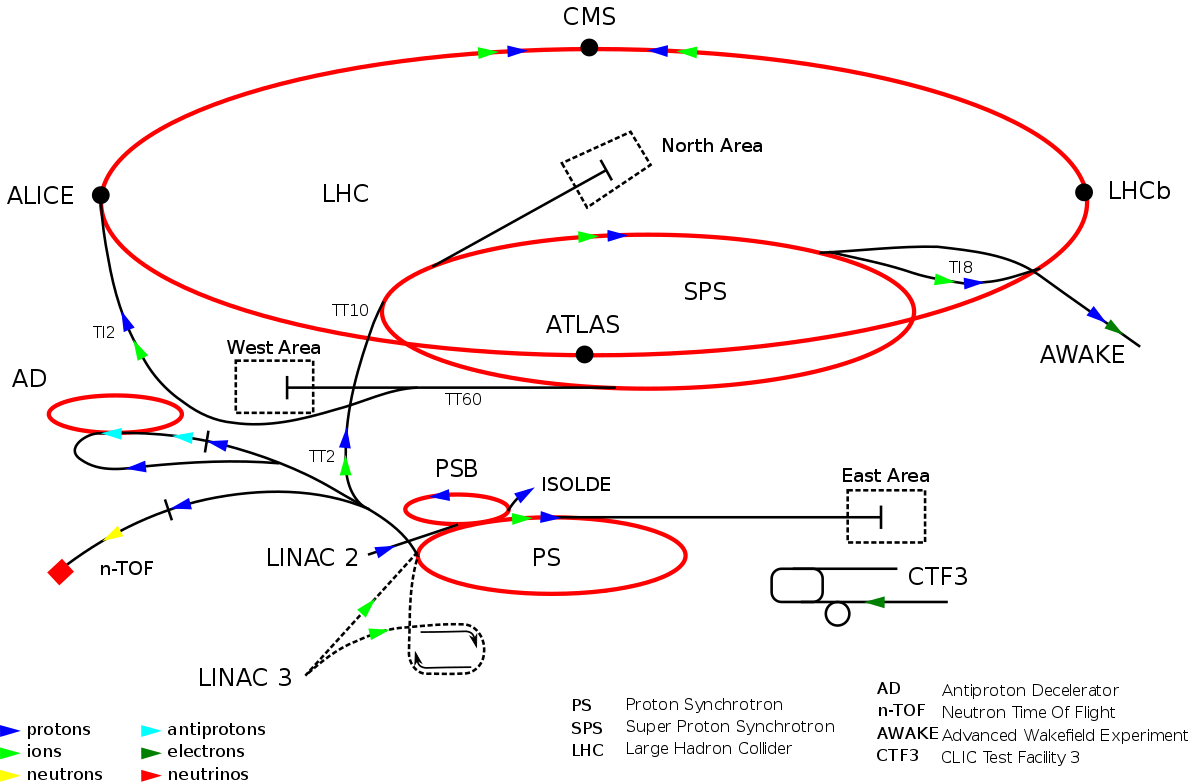
\includegraphics[width=0.8\textwidth]{figures/lhc.png}
    \centering
    \caption{An illustration of the LHC accelerators and the four main experiments.}
    \label{fig:lhc}
\end{figure}

There are 8 interaction regions (IRs) at which two proton beams cross, and protons beams are injected into the LHC from two IRs. Before protons are injected to the LHC, they undergo a multi-stage acceleration by several accelerators~\cite{Bruning:782076}: a linear accelerator (LINAC2), the Proton Synchrotron Booster, the Proton Synchrotron (PS), and the Super Proton Synchrotron (SPS). The proton beams are accelerated up to 450 GeV when they are injected to the LHC with a 25 ns bunch spacing in Run II. There are more than $10^{11}$ protons in each bunch, and the large number of protons in each bunch results in multiple collisions per bunch crossing, knowns as \textit{pile-up}. In 2016, the mean number of interactions per bunch crossing was $\langle\mu\rangle = 24.9$.

The four main experiments at CERN are distributed around the LHC at collision points. Two experiments, ATLAS and CMS, are designed as general purpose experiments, and A large Ion Collider Experiment (ALICE) and the Large Hadron Collider beauty (LHCb) are designed to study strong interaction using heavy ion collisions and the matter-antimatter asymmetry using b quarks, respectively. Figure~\ref{fig:lhc} shows the four main experiments and the accelerators at the LHC.


\section{The ATLAS detector}
\label{sec:atlas:detector}

\begin{figure}[!htb]
    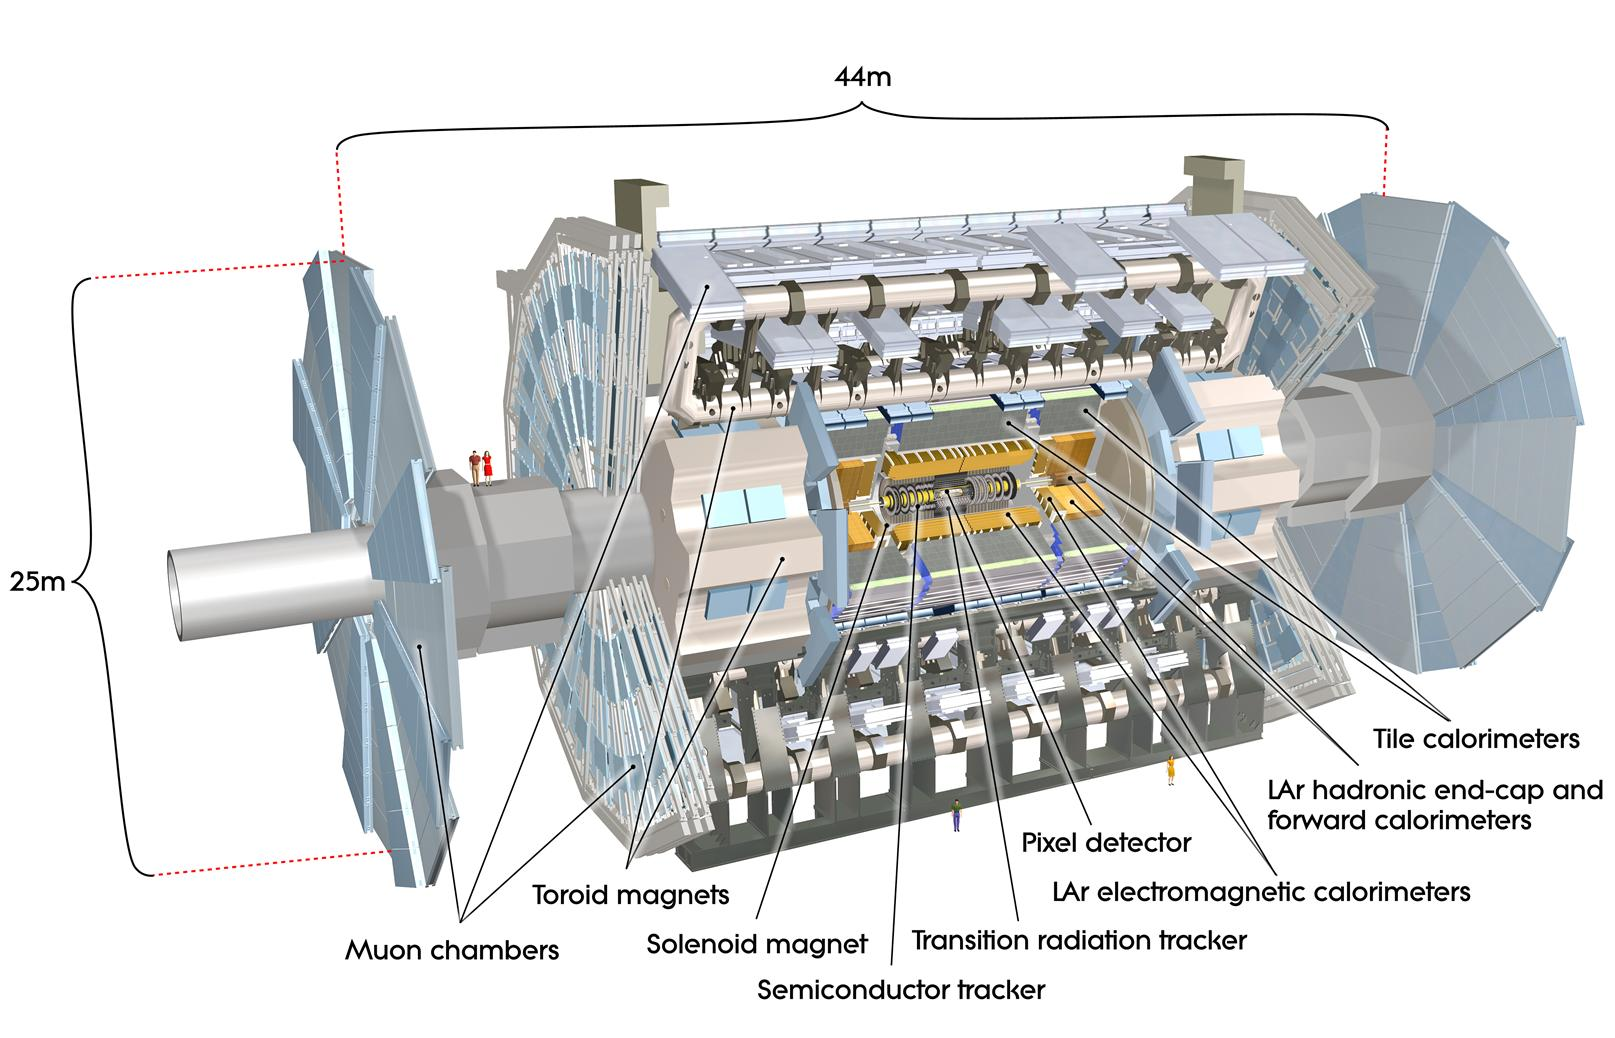
\includegraphics[width=0.8\textwidth]{figures/atlas.png}
    \centering
    \caption{The ATLAS detector showing three sub-detector systems.}
    \label{fig:atlas}
\end{figure}

The ATLAS detector is a multi-purpose detector designed to investigate a wide range of physics, including the search for the Higgs boson in Run I and many searches beyond the SM. The detector measures 46 m long, 25 m in diameter, and it has three main layers of sub-detectors to detect particles created from $pp$ collisions at the Interaction Point (IP). Figure~\ref{fig:atlas} shows the ATLAS detector and the sub-detector systems: the Inner detector, the electromagnetic and hadronic calorimeters, and the muon spectrometer. In this section, the coordinate system, the sub-detectors, and the magnet system of the ATLAS detector are described.

\subsection{Coordinate System}
\label{sec:atlas:coordinate}
In the ATLAS coordinate system, the interaction point (IP) is defined as the origin of the coordinate system. The beam line defines the z-axis, and the x-y plane perpendicular to the beam line is referred to as the transverse plane. The positive x-axis points from the IP to the center of the LHC ring, and the positive y-axis is defined as pointing upward. The azimuthal angle $\phi$ is defined as the angle from the x-axis. The polar angle $\theta$ is defined as the angle from the positive z-axis, and it is also expressed as pseudo-rapidity $\eta$,

\begin{equation}
    \label{eq:eta}
    \eta = -\ln (\tan (\frac{\theta}{2})),
\end{equation}

which is a particularly useful quantity because of Lorentz invariance under a boost along the z axis. The distance $\Delta R$ is defined in $\eta-\phi$ plane as $\Delta R = \sqrt{\Delta \eta^{2} + \Delta \phi^{2}}$.

\subsection{The Inner Detector}
\label{sec:atlas:id}
The Inner Detector (ID) is a particle tracker designed to measure the charge and transverse momentum of charged particles and to reconstruct the primary and secondary vertices. It consists of cylindrical barrels and two end-cap disks from three sub-detectors centered around the IP. The ID covers the pseudo-rapidity region up to $|\eta| < 2.5$. 

The detector is immersed  in a 2 T magnetic field generated by the superconducting solenoid magnets, and the magnetic field is used to bend trajectories of charged particles. The transverse momentum and the charge of a particles are then determined from the curvature of the trajectory.

The sub-detectors of the ID, the Pixel tracker, the semiconductor tracker (SCT), and the transition radiation tracker (TRT), are discussed in the following sections.

\subsubsection{Pixel Detector}
\label{sec:atlas:pixel}

The Pixel detector is a semiconductor detector in the innermost part of the ATLAS tracking system. The detector consists of 4 concentric layers of barrel detectors and 3 disk detectors at each end-cap region. The barrels and disks are made of a rectangular Pixel modules containing $80.4\cdot10^{6}$ pixels of the size 50$\times$400 \si{\micro\meter^{2}} ($6\cdot10^{6}$ pixels of the size 50$\times$250 \si{\micro\meter^{2}} for the IBL)~\cite{1748-0221-10-06-C06012}. As a charged particle traverse through pixels, the currents generated by ionizing electrons are measured and registered as hits. The pixels provide spatial information with resolution of $\sim$ 8 \si{\micro\meter} in radial direction and $\sim$ 75 \si{\micro\meter} in the beam axis, and the information is used for momentum measurements as well as reconstruction of primary and secondary vertices. In Run 2, the Insertable B-Layer (IBL)~\cite{Abbott:2307576} was installed to maintain and improve the performance of the ATLAS detector under increasing pile-up.

\subsubsection{Semi-conductor Tracker}
\label{sec:atlas:sct}

The Semi-Conductor Tracker (SCT) is the next tracking system following the Pixel detector. Similar to the Pixel detector, the SCT consists of 4 layers of barrel detectors and 9 disk detectors at each end-cap region. Each barrel/disk is made of SCT modules containing double-sided silicon strips, measuring 80 \si{\micro\meter} wide and 12 \si{\centi\meter} long\footnote{There are two versions of SCT strips in end-cap modules with lengths of 12 \si{cm} and 7 \si{cm}.}. Strips are positioned parallel (perpendicular) to the beam axis in the barrel (end-cap) region. Because a single strip can only provide spatial information in ($r$-$\phi$) direction in barrel and ($z$-$\phi$) direction in end-cap region, double-sided strips are displaced by a relative angle of 40 \si{\milli\radian} to provide three-dimensional spatial measurements of charged particles. The SCT has a spatial resolution of 17 \si{\micro\meter} in radial direction and 580 \si{\micro\meter} in $z$ direction. The information collected by the SCT is used for charge and transverse momentum measurements and reconstruction of vertices.


\subsubsection{Transition Radiation Tracker}
\label{sec:atlas:trt}

The Transition Radiation Tracker (TRT) is the outermost tracking system in the ID, covering the region up to $|\eta| < $ 2.0. The TRT barrel region is covered by 52,544 straw tubes aligned parallel to the beam axis. The TRT end-cap region is covered by 122,800 straw tubes aligned in radial direction. Each straw tube is filled with a Xe-based gas mixture, and a wire is placed at the center of the tube, acting as an anode. When a charged particle traverses the detector, it ionizes the gas mixture inside straws, producing a cascade of electrons. These electrons from the ionization drift toward the center wire, creating signal for the readout with the intrinsic resolution of a single straw tube of $\sim$120\si{\micro\meter}~\cite{Vogel:1537991}. 

The TRT also provides important information on particle identification. The spaces between straws are filled with polymer fiber (barrels) and foils (end-caps) for the production of transition radiation. When a highly relativistic charged particle passes through them, photons may be emitted by transition radiation, and these photons can be absorbed by the gas mixture, resulting in higher readout signals than usual, called high-threshold hits. The effect is stronger for electrons due to larger relativistic factor ($\gamma = E/m$) than particles with a lower boost such as hadrons. Therefore, the high-threshold hits in the TRT can be used for electron/pion identification~\cite{ATLAS-CONF-2011-128}.

\subsection{The Calorimeters}
\label{sec:atlas:calorimeter}

\begin{figure}[!htb]
    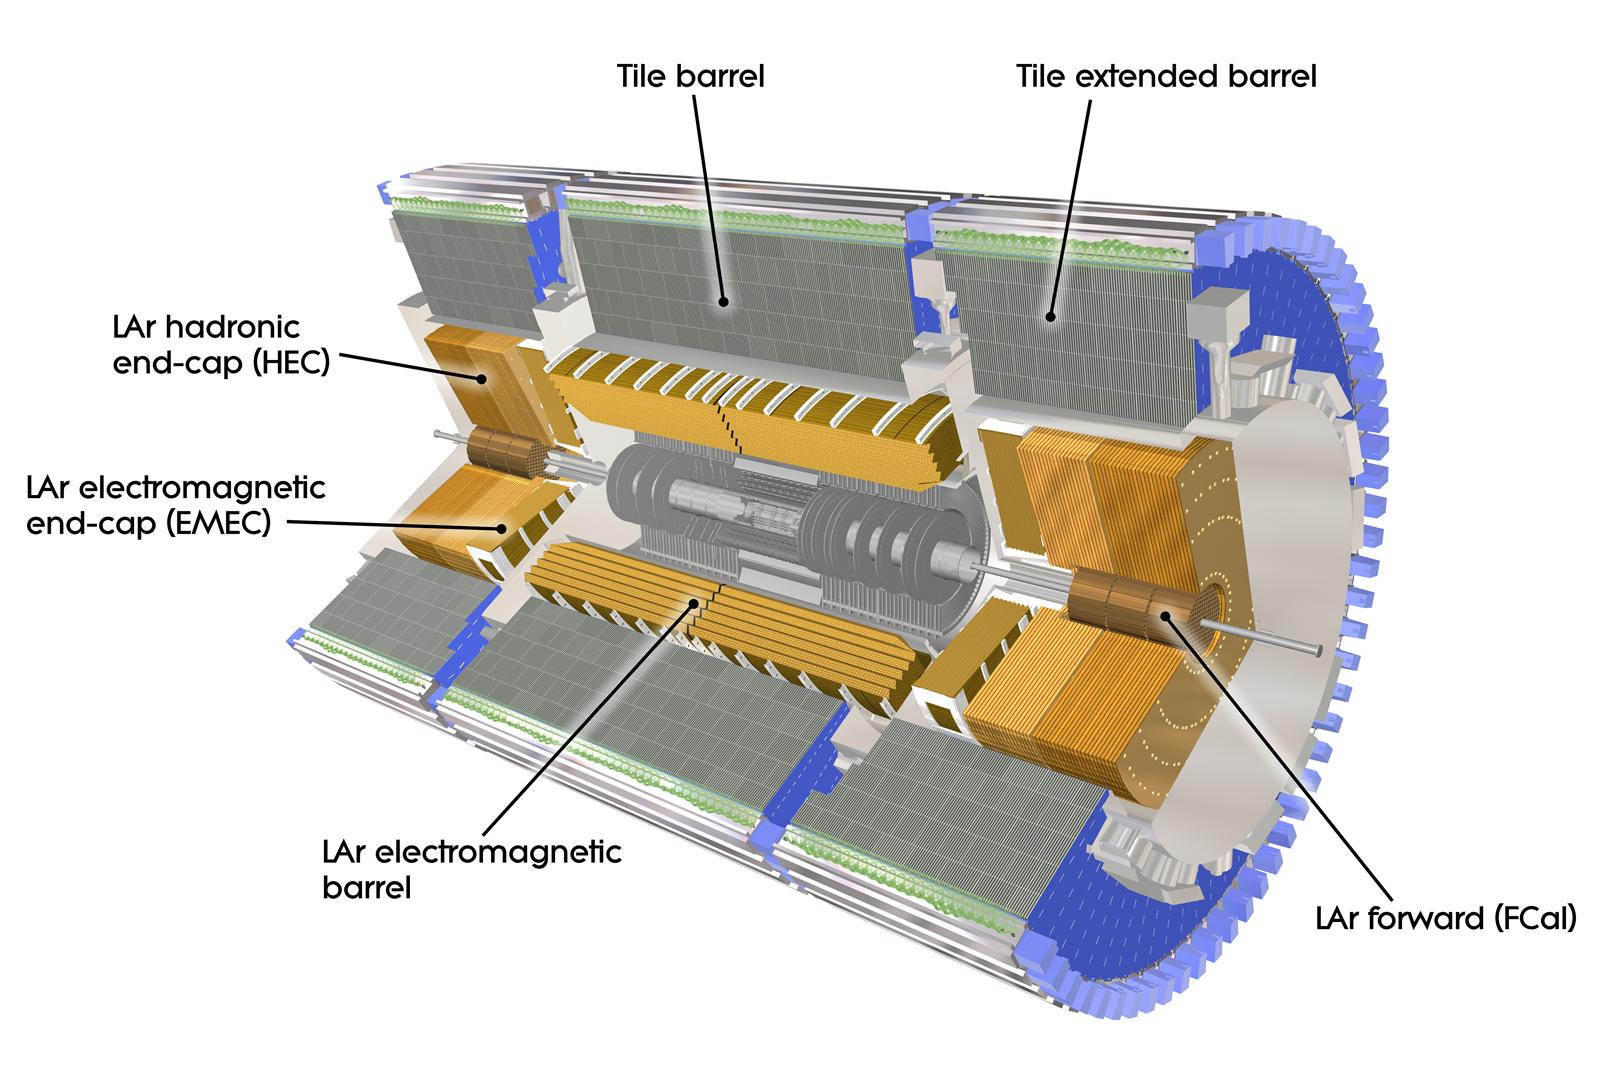
\includegraphics[width=0.8\textwidth]{figures/calorimeter.jpg}
    \centering
    \caption{The ATLAS calorimeter system.}
    \label{fig:calorimeter}
\end{figure}


The ATLAS calorimetry system, shown in Figure~\ref{fig:calorimeter}, consists of two sub-systems, the Liquid Argon (LAr) calorimeters~\cite{1742-6596-293-1-012044} and the tile calorimeters (TileCals)~\cite{HenriquesCorreia:2004868}. The calorimeters are designed to measure the energy deposited by a particle as it traverse through the detector, and the signals from calorimeters are used for the trigger system. Based on its usage, the calorimeters can be grouped into two sets of calorimeters: the Electromagnetic (EM) calorimeters and hadronic calorimeters.


\subsubsection{Electromagnetic Calorimeter}
\label{sec:atlas:EMcal}
The EM calorimeters (EMC) are located outside the ID and the solenoid magnet, and they are designed to measure the energy deposition from electrons and photons. They are composed of two LAr calorimeters, the EM End-Cap calorimeter (EMEC) covering the region of $|\eta|<$ 1.475 and the EM Barrel (EMB) calorimeter covering the region of 1.375 $<|\eta|<$ 3.2. The LAr calorimeters are composed of layers of high density material (Pb) and LAr sampling layer interspaced for absorption of electron/photons and energy measurement, respectively. The first layer of the LAr calorimeters is called \textit{presampler} which is a thin layer of liquid argon without absorber in front, and it is used to correct for the energy loss before a particle reach the calorimeter. The LAr calorimeters are called sampling calorimeters because only a small fraction of the deposited energy is measured by sampling layers.

When an electron or a photon enters the calorimeters, the electron/photon interacts with the absorber layers, creating the initial EM shower via bremsstrahlung and pair-production. The EM shower is amplified and collected by the sampling layers. The EM calorimeters have the minimum number of radiation length of 24 $X_{0}$~\cite{ATLAS-LAR-CALORIMETER}.




\subsubsection{Hadronic Calorimeter}
\label{sec:atlas:Hcal}
Hadrons are less likely to produce bremsstrahlung radiation due to heavier mass, and they can traverse through the EMC without losing significant energy. Therefore, the hadronic calorimeters are located outside the EMC to measure the energy of hadrons penetrating the EMC. The hadron calorimeters are composed of both LAr calorimeters and TileCals.

The hadronic LAr calorimeters consists of two parts, the hadronic end-cap calorimeter (HEC) covering the region of 1.5 $<|\eta|<$ 3.2 and the forward calorimeter (FCAL) covering the region of 3.1 $<|\eta|<$ 4.9. The principal of hadronic LAr calorimeters is the same as EM LAr calorimeters. The HEC is divided into four longitudinal layers with copper absorber. The FCAL consists of one EM layer which uses copper as absorber and two hadronic layers with tungsten as passive material. When a hadron enters the hadronic LAr calorimeters, the particle interacts with nuclei of the absorber material via strong force, creating a hadronic shower. The hadronic shower is sampled by sampling layers.

 TileCals are designed to cover the central barrel region ($|\eta| <$ 1.0) and the extended barrel region (0.8 $<|\eta|$ 1.7). The TileCals are made of alternating layers of iron and scintillating tiles. Hadrons entering the absorber layers produce hadronic showers, and the secondary particles from the showers interact with the scintillating tiles to produce lights. The photons are delivered to photomultipliers via wave-length shifting fibers and registered as calorimeter cluster hit.

The TileCals, combined with the hadronic LAr calorimeters, provide precise measurement of hadrons, jets, taus, and missing transverse energy ($E_{T}^{miss}$).


\subsection{The Muon Spectrometer}
\label{sec:atlas:ms}

\begin{figure}[!htb]
    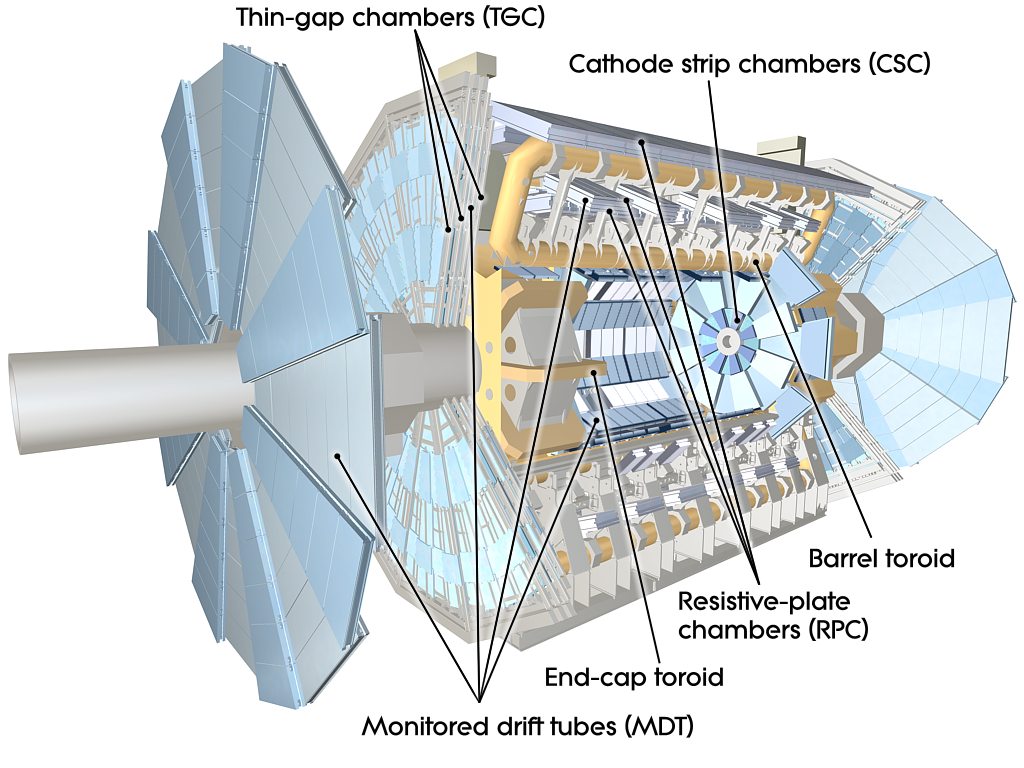
\includegraphics[width=0.7\textwidth]{figures/ms.png}
    \centering
    \caption{The ATLAS Muon Spectrometer}
    \label{fig:ms}
\end{figure}
The Muon Spectrometer (MS) is the outermost detector in the ATLAS detector, responsible for muon identification, momentum measurements, and muon trigger information. The MS is designed to provide high $p_{T}$ momentum measurement with resolution of $\sigma_{p_{T}} / p_{T} = 10\%$, independent from the ID. The MS consists of four sub-detector systems. The Resistive Plate Chambers (RPCs) and the Thin Gap Chambers (TGCs) are used for muon triggering. The Monitored Drift Tubes (MDTs) and the Cathode Strip Chambers (CSCs) allow precise tracking and momentum measurements. The MS barrel region covers the region of $|\eta|<$ 1, and the coverage is extended to $|\eta|<$ 2.7 in the end-cap. The magnetic field is applied with an average 0.5 T~\cite{ARNAUD2008265} by a system of a large toroidal magnet (barrel) and two smaller toroidal magnets (end-cap). A layout of the MS is shown in Figure~\ref{fig:ms}.

\subsubsection{Monitored Drift Tube Chambers}
\label{sec:atlas:mdt}

The MDT chambers provide precision momentum measurements using chambers of drift tubes filled with a gas mixture of Ar (97\%) and $\mathrm{CO}_{2}$(3\%). The barrel MDT chambers are arranged in three layers, covering the region of $|\eta|<$ 1.1. The end-cap MDT chambers are arranged in three wheels, covering the region of 1.1 $<|\eta|<$ 2.7. Each drift tubes measures 3 \si{\centi\meter} in a diameter, and a tungsten-rhenium wire is placed at the center as an anode. Each chamber has 6-8 layers of drift tubes. The principal of particle detection is similar to the TRT, but the drift tubes are arranged perpendicular to the beam axis in the barrel layers and tangential in the end-cap layers. This configuration allows the MDT to measure the curvature of a muon in $\eta$-$z$ plane under the toroidal magnetic field.

\subsubsection{Cathode Strip Chambers}
\label{sec:atlas:csc}

The CSCs are located on the innermost wheel of the end-caps, covering the region of 2.0 $<|\eta|<$ 2.7. In this region, the MDTs would not operate properly due to the high rates of muons coming from the beam pipe. Instead, sixteen CSCs on each end-cap provide precise tracking for high density muons with the resolution of 60 \si{\micro\meter} in $\eta$-$z$ plane and 5 \si{\milli\meter} in the radial direction. The CSCs are multi-wire proportional chambers with segmented cathode strips in alternating alignment. The multi-wires are aligned in the radial direction, and the strips are aligned perpendicular or parallel to the wires to provide 2 dimensional measurements in both $\eta$ and $\phi$ directions.


\subsubsection{Resistive Plate Chambers}
\label{sec:atlas:rpc}

The RPCs provide trigger capability for the muon trigger and measurements in $\eta$, $\phi$ coordinates in the barrel region. There are three RPCs arranged in concentric cylindrical shells around the beam axis. The two inner RPCs are placed at the radii of 5 \si{\meter} and 7.5 \si{\meter} to provide the low-$p_{T}$ trigger information. The outer RPCs are installed at the radius of 10 \si{\meter} to provide high-$p_{T}$ trigger information. Each chamber consists of two parallel resistive plots separated by a 2 \si{\milli\meter} gap filled with a gas mixture based on $\mathrm{C}_{2}\mathrm{H}_{2}\mathrm{F}_{4}$. A muon track passing through the RPCs ionizes the gas, and the signal is multiplied and read out by each chamber, providing 6 measurements for each track.

\subsubsection{Thin Gap Chambers}
\label{sec:atlas:tgc}

The TGCs are designed to provide trigger information and $\phi$ measurements (non-bending direction) in the end-cap region. Similar to the CSCs, the TGCs are made of multi-wire proportional chambers filled with a gas mixture of 55\% $\mathrm{CO}_{2}$ and 45\% $\mathrm{C}_{5}\mathrm{H}_{12}$. The strips are oriented in radial direction, allowing measurements in $\phi$. The TCGs consists of 4 layers of chambers on each end-cap, covering the region of 1 $<|\eta|<$ 2.7.


\subsection{The ATLAS Magnet}
\label{sec:atlas:magnet}

The ATLAS detector has three major superconducting magnet systems surrounding the ID and the MS: the Central Solenoid magnet and the Barrel/End-cap Toroid magnets.

\subsubsection{Central Solenoid Magnet}
\label{sec:atlas:solenoid}
The Central Solenoid magnet surrounds the ID, producing a 2 T magnetic field. The solenoid is designed to bend the trajectory of a charged particle in $r$-$\phi$ plane. The curvatures of charged particles are used for the measurements of charge-to-momentum ratio. The solenoid magnet measures 2.4 \si{\meter} in diameter and 5.3 \si{\meter} in length, and 7.73 \si{\kilo\ampere} of current is applied to generate the solenoidal magnetic field.


\subsubsection{Toroid Magnets}
\label{sec:atlas:toroid}

In the outer region of the ATLAS detector, two superconducting toroid magnet systems are used to generate a magnetic field within the MS. The Barrel Toroid are composed of 8 separate coils made of Al/NbTi/Cu conductor with 120 turns. The toroid measures 20.1 \si{\meter} in diameter and 25.3 \si{\meter} in length. The End-cap Toroid has 8 coils with 116 turns, and the coils are made of the same material as the Barrel Toroid. The nominal current of 20.5 \si{\kilo\ampere} is applied to generate a magnetic field in the range of 1 to 2 T with the field integral between 2 to 8 Tm.

\section{The ATLAS Trigger System}
\label{sec:atlas:daq}

\begin{figure}[!htb]
    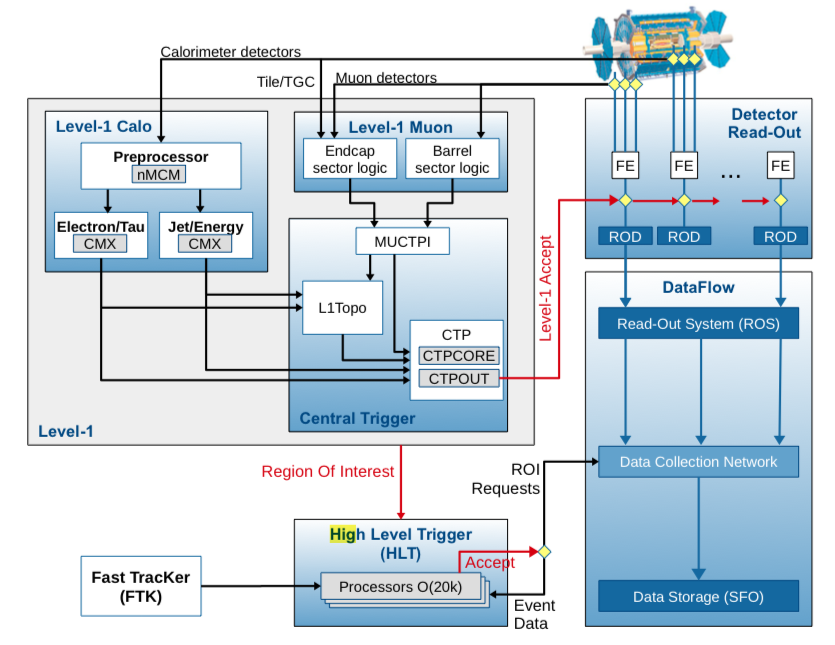
\includegraphics[width=0.8\textwidth]{figures/tdaq.png}
    \centering
    \caption{Layout of the ATLAS Trigger and data acquisition system in Run 2.}
    \label{fig:tdaq}
\end{figure}

The ATLAS trigger system is designed to select interesting events from raw event data at high rate, generated by $pp$ collisions. In Run 2, the LHC collide proton bunches every 25 \si{\nano\second}, resulting in about a billion $pp$ collisions per second at $\langle\mu\rangle = 24.9$ (in 2016). Due to the limited bandwidth and computing resources, it is impossible to record all events from the collisions. Therefore, the ATLAS trigger system is implemented to reduce the data taking rate from 40 \si{\mega\hertz} to 100 \si{\kilo\hertz}. In Run 2,several upgrades have been performed in both hardware and software to maintain data quality in the environment with increasing pile-up, higher instantaneous luminosity at the center-of-mass energy of $\sqrt{s}=$13 TeV.

The trigger system in Run 2 consists of a hardware-based Layer 1 (L1) trigger and a software-based High Level Trigger (HLT). Figure~\ref{fig:tdaq} shows the ATLAS trigger and data acquisition system in Run 2. The events accepted by the trigger system are further processed by the Data Acquisition (DAQ) system where the information from front-end electronics of each detector component are used to build an individual event. The reconstructed events from DAQ are sent to Data Storage (SFO) for permanent storage.



\subsection{Level 1 Trigger}
\label{sec:atlas:l1trigger}

The L1 trigger is a hardware-based trigger system that operates at the maximum rate of 100 \si{\kilo\hertz}~\cite{1742-6596-762-1-012003}. The main components of the L1 trigger consist of the L1 calorimeter trigger system and the L1 muon trigger system . The L1 trigger uses custom electronics to make fast decisions and find regions of interest (RoI) in the detector where potentially interesting activities are registered in the calorimeters or the MS.

A list of trigger selection is developed based on the physics goal of the collaboration and the needs of individual analyses. The list is called the Trigger Menu~\cite{VazquezSchroeder:2287548}. The L1 trigger accepts the events with high $p_{T}$ tracks, jets, or large $E_{T}^{miss}$ that satisfies one of the trigger menu. The events accepted by the L1 trigger is passed to the software-based trigger system.


\subsection{High Level Trigger}
\label{sec:atlas:hlt}

In Run 2, two software-based trigger systems, the Level 2 trigger and the Event Filter, are combined into a single software trigger system, called the High Level Trigger(HLT) . The HLT makes the decision on events based on full information from the detector read-out in the RoI passed by the L1 trigger. This includes a fast reconstruction of the inner detector tracks. The HLT has the average output rate of 1 \si{\kilo\hertz}~\cite{1742-6596-762-1-012003}, constrained by data storage limitation. 



\chapter{Z' Reconstruction}
\label{chap:reco}

The experimental signature in the search for long-lived $Z'$ is characterized by a dilepton vertex with high $p_{T}$ leptons, displaced ($>$ 2~\si{\milli\meter}) from the primary vertex in transverse plane, referred a \textit{displaced vertex}. In this chapter, the reconstruction of displaced vertices in the ATLAS ID is described.

\section{Track Reconstruction in the Inner Detector}
\label{sec:reco:track}

Track reconstruction in the ATLAS uses pattern recognition algorithms to reconstruct the trajectories of charged particles, referred as a \textit{track}. When a charged particle traverse through the ID, the particle interact with the sub-detectors of the ID (Pixel, SCT, and TRT), leaving raw detector signals. The raw signals are digitized and registered as detector \textit{hits}, and these detector hits are used for track reconstruction. 

\subsection{Standard Tracking}
\label{sec:reco:st}


\begin{figure}[!htb]
    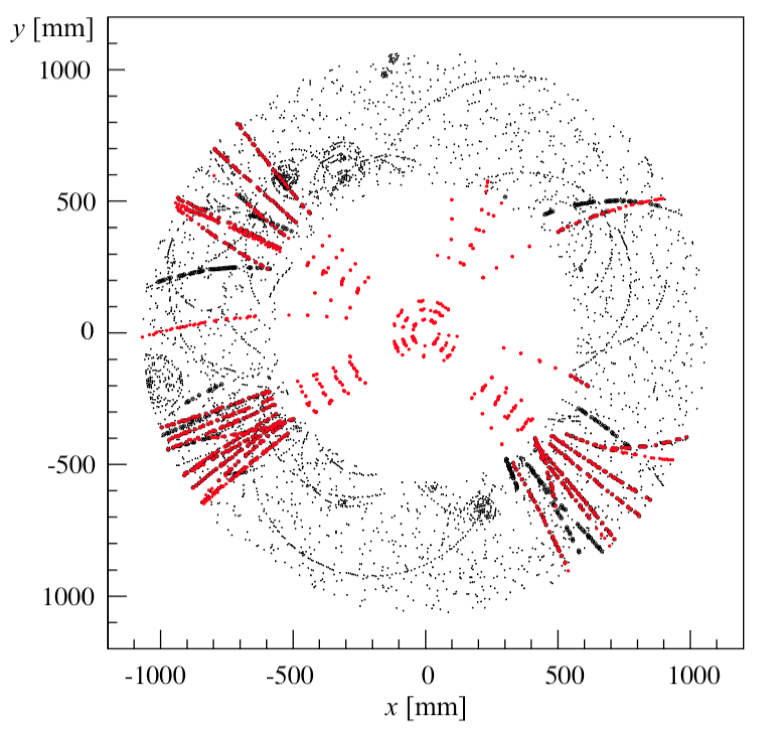
\includegraphics[width=0.6\textwidth]{figures/tracking.png}
    \centering
    \caption{Illustration of detector hits and reconstructed tracks in the ID. The bright colors represent the detector hits associated with reconstructed tracks.}
    \label{fig:tracking}
\end{figure}

The standard ATLAS track reconstruction is the main track reconstruction algorithm used in the ATLAS experiment. In the first stage of the track reconstruction, detector hits from the Pixel or the SCT detector are used to create \textit{track seeds}, collections of silicon hits used for the initial track finding. If a track seed passes certain quality criteria, including a $p_{T}$ and impact parameter selection, the track seed is extended to the outer part of the ID using a window search and pattern recognition algorithms. The extended tracks are evaluated based on $p_{T}$, number of hits, and impact parameters, and only the tracks satisfying the standard track selections are stored in the track collection. Figure~\ref{fig:tracking} illustrates detector hits and reconstructed tracks in the ID. The important standard track selections is summarized in Table~\ref{table:tracking}~\cite{ATL-PHYS-PUB-2017-014}.


Tracks are described by five parameters (helix) and a reference point, using a perigee representation~\cite{Akesson:973401}. The parameters are the transverse (longitudinal) impact parameter $d_{0}$ ($z_{0}$), the azimuthal angle $\phi$, the polar angle $\theta$, and the charge-to-momentum ratio, $q/p$. The average position of the $pp$ interaction, referred as beamspot position, is used as the reference point for the track representation~\cite{Aaboud:2016rmg}.


\begin{table}[!htb]
  \centering
  \begin{tabular}{ c  c  c }
    \hline
    \hline
    & Standard & Large radius \\ [0.5ex]
    \hline
    Maximum $d_{\rm{0}}$ (mm) & 10 & 300 \\
    Maximum $z_{\rm{0}}$ (mm) & 250 & 1500 \\
    Maximum $|\eta|$ & 2.7 & 5 \\
    Maximum shared silicon modules & 1 & 2 \\
    Minimum unshared silicon hits& 6 & 5 \\
    Minimum silicon hits & 7 & 7\\
    \hline
    \hline
  \end{tabular}
  \caption{Main track selection in the standard and large radius tracking algorithms.}
  \label{table:tracking}
\end{table}


\subsection{Large Radius Tracking}
\label{sec:reco:lrt}

The standard track reconstruction is proven to be very efficient in Run 2 with the tracking efficiency > 90\%~\cite{Aaboud:2017all}. However, the tracking algorithm is optimized for charged particles promptly produced from the primary interaction, and the strict requirements on the impact parameters, \dzero and \zzero, limit the tracking efficiency for charged particles with large impact parameters ($|d_{0}|$ > 2 mm). Therefore, a dedicated track reconstruction algorithm, referred to as the large radius tracking (LRT), is developed to improve the track reconstruction efficiency for the tracks highly displaced from the primary vertex.

The LRT is performed in a sequence, following the standard tracking. It follows the same reconstruction strategy as the standard tracking, but there are a few important differences between the standard tracking and the LRT:

\begin{itemize}
	\item The pattern recognition algorithms in the LRT only uses \textit{un-used} hits, the silicon hits that have not been used in the standard tracking, in creating and extending track seeds.
	\item The requirements on tracks such as $d_{0}$, $z_{0}$, and number of hits are relaxed.
\end{itemize}

Tracks reconstructed by the LRT using un-used hits are required to pass certain criteria such as minimum $p_{T}$ and number of detector hits, and the selected tracks are merged into the standard track collection for the next step of reconstruction. The track selections in the LRT are summarized and compared with the standard track reconstruction in Table~\ref{table:tracking}. The combined track collection is used as an input for the lepton reconstruction and identification and secondary vertex reconstruction. More details on the LRT can be found in Ref.~\cite{ATL-PHYS-PUB-2017-014}.

Combined with the standard track reconstruction, the LRT provides overall efficiency of $> 90\%$ for the particles that satisfy the fiducial selections in Table~\ref{table:TechEffTable} with a displacement in the transverse plane up to 300 \si{\milli\meter}.

\begin{table}[!htb]
\centering
\begin{tabular}{ r c l }
 \hline
 \hline
  \multicolumn{3}{c}{Fiducial Selections}  \\
 \hline
 $r_{\rm prod}$ & $<$ & 300~mm \\
$|\eta|$ & $<$ & 5 \\
 $\pt$ & $>$ & 1~GeV  \\
 Number of silicon hits & $\ge$ & 7  \\
\hline
\hline
\end{tabular}
\caption{Fiducial selections on particles for tracking efficiency measurements.}
\label{table:TechEffTable}
\end{table}


\section{Electron Reconstruction}
\label{sec:reco:lep}

Electrons are characterized by energy deposits in the EM calorimeter and the associated reconstructed tracks in the ID. The electron reconstruction algorithm uses the energy deposits with total transverse energy $>2.5$~\si{\GeV} in a window of 0.075$\times$0.125 in ($\eta$,$\phi$) to reconstruct EM clusters. The EM clusters are associated with tracks within the same RoI, $|\Delta\eta|<0.05$ and $|\Delta\phi|<0.1$ where the effect of bremsstrahlung is taken into account~\cite{Aad:2014fxa}. In the absence of a matching track, the EM cluster is classified as a photon candidate. The associated pairs of tracks and energy clusters are refitted to improve the energy resolution of the electron candidate. Additional electron requirements, including likelihood-based identification criteria, are imposed on the electron candidates to reduce misidentification.

%By default, electrons are required to have a minimum number of pixel hits and small transverse impact parameters. This is not optimal for the searches that aim to detect displaced vertices as the decay products of displaced vertices tend to have large impact parameters (\dzero, \zzero) and missing hits in the inner layers of the detector. Therefore, these requirements are removed in this analysis.

\section{Muon Reconstruction}
\label{sec:reco:muon}

Muons deposit very little energy in the calorimeter as they traverse through the detector due to the relatively larger mass, given that the probability of bremsstrahlung is $\propto 1/m^{2}$. However, they leave tracks in both the ID and the MS, referred as inner detector (ID) tracks and muon standalone (MS) tracks. The muon reconstruction algorithm uses MS tracks as seeds, and the MS tracks are extrapolated to the ID for the association with ID tracks. A \textit{combined muon} track is created if a MS track is successfully associated with an ID track after the momentum correction for the energy loss from the interaction with the detector material. There are other types of reconstructed muons such as standalone muons, segment-tagged muons, and calorimeter-tagged muons~\cite{Aad:2016jkr}. However, these types of muons are not considered in this analysis as they do not have associated ID tracks which are required for the reconstruction of displaced vertices.

By default, muons are required to have a minimum number of pixel and SCT hits, as well as small transverse impact parameters. This is not optimal for the searches that aim to detect displaced vertices as the decay products of displaced vertices tend to have large impact parameters (\dzero, \zzero) and missing hits in the inner layers of the detector. Therefore, the requirements on \dzero and pixel hits are removed. Also minimum SCT hits on muon tracks are lowered to 2.

\section{Secondary Vertex Reconstruction}
\label{sec:reco:dv}

\begin{figure}[!htb]
    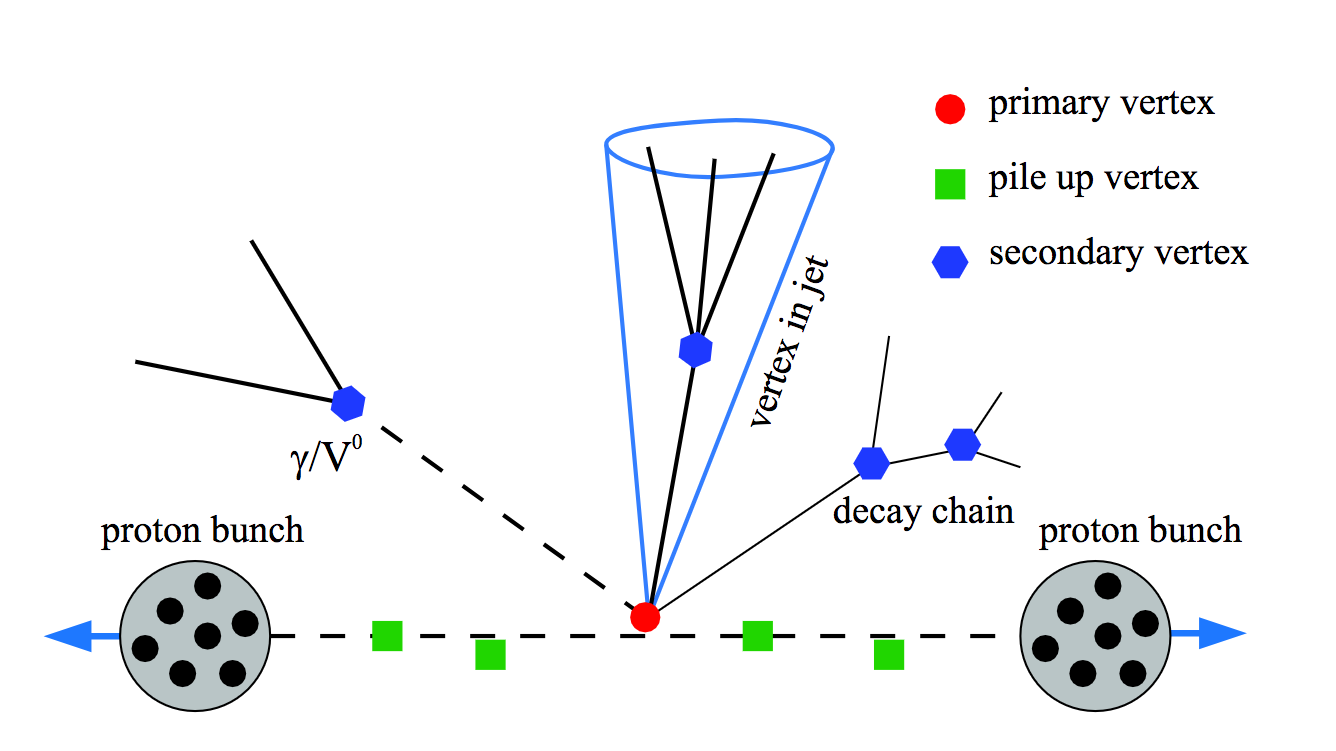
\includegraphics[width=0.6\textwidth]{figures/vertex.png}
    \centering
    \caption{Main vertex topologies in $pp$ collisions: primary, pile-up, and secondary vertices.}
    \label{fig:vertex_topology}
\end{figure}

In the LHC, when two proton bunches collide, several different vertex topologies arise. The primary vertex and several pile-up vertices are formed along the beam line, and the vertices from photon conversion or long-lived particles are formed displaced from the primary vertex as shown in Figure~\ref{fig:vertex_topology}. These displaced vertices are referred as secondary vertices. In the search for long-lived $Z'$ in the dilepton decay channel, the decay products of long-lived particles can be reconstructed as a secondary vertex.

The secondary vertex reconstruction is based on the primary vertex reconstruction algorithm~\cite{1742-6596-119-3-032033} and was originally developed for the study of material mapping of the ID in Run I. The algorithm was updated for several long-lived particle searches in Run 2.

In the first stage, track are selected using the requirements on track parameters and hit patterns shown in Table~\ref{table:vertex_track_selection_simple}. In addition, tracks are required to have $p_{T} >$ 1 GeV to reduce low $p_{T}$ tracks from a photon conversion, and track quality requirement is relaxed ($\chi^{2} / DOF < $ 50) to improve the efficiency of reconstructing displaced vertices. The tracks reconstructed by both the standard track reconstruction and the LRT are used as input. The tracks passing the track requirements are used to create two-track vertices, based on the closeness of two tracks in space. This process results in a large number of fake vertices. The fake vertices are rejected by considering the location of a vertex and hit patterns of the tracks associated with the vertex. A vertex is rejected if the associated tracks have any hits at a radius smaller than the vertex position. Two-track vertices passing the fake rejection are refitted using a Kalman Filter~\cite{Kalman:434680} for precise vertex position measurements, and track parameters are calculated with respect to the secondary vertex.

The two-track vertices reconstructed by the secondary vertex reconstruction serve as the primary analysis object in this thesis. %Section~\ref{sec:vertex_selection} discusses the vertex selection applied to these two-track vertices to select displaced vertices. Lepton identification requirements are applied to the tracks from secondary vertices after applying analysis level vertex selection, so secondary vertices reconstructed can have any combination of muon, electron, or non-leptonic tracks.







\begin{table}[!htb]
  \centering
  \begin{tabular}{ l c }
    \hline
    \hline
	Variable      		& Cut                                         	\\
    \hline
	$p_{T}$ (GeV)		& $>$ 1.0										\\
	$\chi^{2} / DOF$	& $<$ 50  										\\
	$d_{0}$	(mm)		& 2.0 - 300.0									\\
	$z_{0}$ (mm)		& $<$ 1500.0									\\
	SCT hits			& $\geq$ 2										\\
	Si shared hits	    & $\leq$ 2										\\
	Pixel and TRT hits  & TRT hits > 0 or Pixel hits $\geq$ 2			\\
    \hline
    \hline
  \end{tabular}
  \caption{Track requirements for secondary vertex reconstruction.}
  \label{table:vertex_track_selection_simple}
\end{table}



\chapter{Analysis Overview}
\label{chap:analysis_overview}

This thesis presents a search for a heavy long-lived resonance decaying to a dilepton pair, \mumu, \ee, or \emu within the ATLAS Innder Detector. The analysis uses 32.8 $\mathrm{fb^{-1}}$ of $pp$ collision data at $\sqrt{s}=13$ TeV collected in 2016 in the ATLAS experiment. The long-lived particle (LLP) is referred as $Z'$ but with no assumption on $Z'$ production mechanism for a model-independent search.

There have been several searches for the LLPs produced in $pp$ collisions in Run I at $\sqrt{s} =$ 8 TeV, including the search for displaced hadronic jet~\cite{Blackburn:1550730}, displaced heavy flavors~\cite{Harris:1512932}, or multi-track displaced vertex~\cite{Aad:2015rba}, and no significant excess was observed. The signature considered in this analysis is distinct from the previous searches, and it is one of the first efforts in the ATLAS experiment to search for a genetic displaced vertex signature decaying to a dilepton pair. This analysis focuses on interpreting the LLPs decaying to displaced dilepton vertices in the context of model-independent, exotic resonance search.

In this search, a special setup (described in Section~\ref{sec:reco:lrt}) of data reprocessing and reconstruction is used in order to gain sensitivity for the non-conventional signature of LLPs. The special setup allows the reconstruction of tracks with large impact parameters and secondary vertices significantly displaced from primary vertices. 

\chapter{Data and MC Samples}
\label{chap:data_mc}

\section{Data Samples}
\label{sec:data_mc:data}

The analysis uses the 2016 $pp$ collisions data (periods A-L) with the integrated luminosity of 32.8 $\mathrm{fb^{-1}}$. In this search, because the standard ATLAS track reconstruction does not provide good sensitivity for long-lived particles, a dedicated data \textit{stream}, \texttt{DRAW\_RPVLL}, is used to reconstruct events using the non-standard reconstruction as described in Chapter~\ref{chap:reco}. The stream is used in several Exotics and SUSY analyses, searching for long-lived particles. %non-standard reconstruction objects.

In this stream, a subset of events from the \textit{main} physics stream~\cite{Aaboud:2016leb}, a data stream used for common physics analyses in ATLAS, is selected by a set of offline filters, called \texttt{RPVLL} filters. The filters select events using the HLT and offline selections configured for each analysis. The triggers and offline selection used in this search is discussed in Chapter~\ref{chap:signal_selection}. The selected events are passed downstream for reconstruction. The data is in \texttt{RAW} format so that low-level information such as detector hits can be used for the special reconstruction algorithms to reconstruct displaced tracks and vertices.

The events passing HLTs are processed by a sequence of reconstruction algorithms with varying configurations, and the ATLAS metadate interface (AMI) tags are used to specify the configurations to be used for a data processing chain. In this analysis, the events are centrally processed with AMI tag \texttt{r8669} in which the dedicated track reconstruction algorithm, the LRT, and the secondary vertex reconstruction algorithm are enabled to reconstruct tracks and vertices, respectively. The output of \texttt{DRAW\_RPVLL} stream is in \texttt{DAOD\_RPVLL} format which is a standard \texttt{xAOD} data format with additional displaced tracks and secondary vertices reconstructed. 

The \texttt{DAOD\_RPVLL} is further processed to produce the \texttt{DAOD\_SUSY15} derivation for data reduction and software fixes on analysis objects such as energy calibration\footnote{Software fixes are released by the ATLAS collaboration in the form of \texttt{AODfix}.}, as recommended by the Analysis Model Study Group (AMSG)~\cite{Catmore:1543445}. Table~\ref{table:data_samples} summarizes datasets used in this search.

\begin{table}[!htb]
  \centering
  \resizebox{\textwidth}{!}{
    \begin{tabular}{ l l }
      \hline
      \hline
      Format     				& Dataset       													\\
      \hline
      \texttt{DRAW\_RPVLL}	& data16\_13TeV.*.physics\_Main.merge.DRAW\_RPVLL.f*\_m*			\\
      \texttt{DAOD\_RPVLL}	& data16\_13TeV.*.physics\_Main.recon.DAOD\_RPVLL.f*\_r8669			\\
      \texttt{DAOD\_SUSY15}	& data16\_13TeV.*.physics\_Main.recon.DAOD\_RPVLL.f*\_r8669\_p3185	\\
      \hline
      \hline
    \end{tabular}
  }
  \caption{Dataset used in \texttt{DRAW\_RPVLL}, \texttt{DAOD\_RPVLL}, and \texttt{DAOD\_SUSY15} format.}
  \label{table:data_samples}
\end{table}

This search uses a modified version of the standard \texttt{GoodRunsList} because a small number of events selected by \texttt{DRAW\_RPVLL} were not reconstructed successfully. The corresponding luminosity blocks were removed from the \texttt{GoodRunsList}\footnote{\url{data16\_13TeV.periodAllYear\_DetStatus-v83-pro20-15\_DQDefects-00-02-04\_PHYS\_StandardGRL\_All\_Good\\\_25ns\_DAOD\_RPVLL\_r8669.xml}}.


The tag and probe studies of Section~\ref{sec:trigger_efficiency} are performed on the standard xAOD dataset using derivations of the performance groups, given in Table~\ref{table:data_samples:tag_probe}.  

\begin{table}[!htb]
  \centering
  \resizebox{\textwidth}{!}{
    \begin{tabular}{ l l }
      \hline
      \hline
      Format     				& Dataset       													            \\
      \hline
      \texttt{DAOD\_EGAM1}	& data16\_13TeV.*.physics\_Main.PhysCont.DAOD\_EGAM1.grp16\_v01\_p3013    \\
      \texttt{DAOD\_MUON1}	& data16\_13TeV.*.physics\_Main.PhysCont.DAOD\_MUON1.grp16\_v01\_p3043	\\
      \hline
      \hline
    \end{tabular}
  }
  \caption{Datasets used for tag and probe studies.}
  \label{table:data_samples:tag_probe}
\end{table}



\section{MC Samples}
\label{sec:mc_sample}

\subsection{Signal Samples}
\label{sec:signal_sample}
The long-lived $Z'$ is generated using \pythia 8.1/8.2~\cite{1126-6708-2006-05-026} with the \texttt{NNPDF23LO} PDF set~\cite{Ball:2014uwa} and the min-bias tune \texttt{A14}. In this signal samples, $Z'$ is singly produced from $q\bar{q}$ scattering and decays to a $\mu\mu$, $ee$, or $e\mu$ pair. The proper lifetime, $c\tau$, is set to 100, 250, or 500 mm. The mass of $Z'$ is set between 100 and 1000 GeV. A width based on relativistic Breit-Wigner is assumed for the new resonance. A sample of 20k events are generated for each mass and lifetime. Table~\ref{table:MC_signal_samples} summarizes dataset identifiers (DSID), mass, width, and lifetime of the signal MC samples used in this search.

\begin{table}[!htb]
  \centering
  \begin{tabular}{ c c c c c c c }
    \hline
    \hline
           &   &    & \multicolumn{3}{c}{DSID}                 \\
    $m_{Z'}$ (GeV) & $\Gamma$ (GeV) & $c\tau$ (mm) &$\mu\mu$ & $ee$ & $e\mu$ \\
    \hline
    100			   &	2.8         &   100	& 308264	& 309539		&	309554		\\
    100			   &	2.8         &   250	& 308265	& 309540		&	309555		\\
    100			   &	2.8         &   500	& 308266	& 309541		&	309556		\\
    250			   &   6.9	        &   100	& 301911	& 309542		&	309557		\\
    250			   &	6.9         &   250	& 301912	& 309543		&	309558		\\
    250			   &	6.9         &   500	& 301913	& 309544		&	309559		\\
    500			   &   14.7         &   100	& 301914	& 309545		&	309560		\\
    500			   &	14.7        &   250	& 301915	& 309546		&	309561		\\
    500			   &	14.7        &   500	& 301916	& 309547		&	309562		\\
    750			   &	23.0        &   100	& 308285	& 309548		&	309563		\\
    750			   &	23.0        &   250	& 308286	& 309549		&	309564		\\
    750			   &	23.0        &   500	& 308287	& 309550		&	309565		\\
    1000	       &	31.0        &   100	& 301917	& 309551		&	309566		\\
    1000	       &	31.0        &   250	& 301918	& 309552		&	309567		\\
    1000	       &	31.0        &   500	& 301919	& 309553		&	309568		\\
    \hline
    \hline
  \end{tabular}
  \caption{Mass, lifetime, and DSID of the signal MC samples.}
  \label{table:MC_signal_samples}
\end{table}

The signal MC samples generated using \pythia are processed to include detector simulation using the AMI tags \texttt{s2698} and \texttt{s2726}. The samples are overlaid with simulated minimum-bias events to model multiple interactions (pile-up) in data samples. In the signal MC samples, the average pile-up, denoted as $\langle\mu\rangle$, ranges from 10 to 40 with small number of events having $\langle\mu\rangle$ < 10. The difference in the $\langle\mu\rangle$ distributions between MC and data samples are corrected for by pile-up reweighting. The resulting MC samples are reconstructed using AMI tag \texttt{r8788}.

In the reconstruction process, the LRT and the secondary vertex reconstruction algorithms are used with the same configuration as data samples to reconstruct displaced tracks and vertices. The reconstructed events are stored in \texttt{DAOD\_RPVLL}, and the samples are processed to produce the \texttt{DAOD\_SUSY15} derivation for data reduction and software fixes on analysis objects.

The representative plots of generator-level $p_{T}$ and $\eta$ distributions of $Z'$ and the muons from the decay of the $Z'$, referred as \textit{signal} muons, are shown in Figure~\ref{fig:truth_zp_muon} using the signal MC samples with $m=$ 500, 1000 GeV and $c\tau=$ 100 mm. %The signal MC samples with $ee$ and $e\mu$ final states produce similar distributions as shown in Appendix~\ref{app:signal_truth}.

%The $\eta$ distribution of $Z'$ shows a forward distribution, and it is reweighted to a flat $\eta$ distribution to provide model-independent result. The details are discussed in Section~\ref{sec:efficiency_reweighting}.
The $\eta$ distribution of signal muons shows that most of the signal muons are produced within the detector acceptance ($|\eta| <$ 2.7). The characteristic upper edge in the $p_{T}$ spectrum is related to the $Z'$ mass.
%The $p_{T}$ distribution of muons shows that muon $p_{T}$ is constrained by the $Z'$ mass.


\begin{figure}[!htb]
    \centering
    \subfloat[]{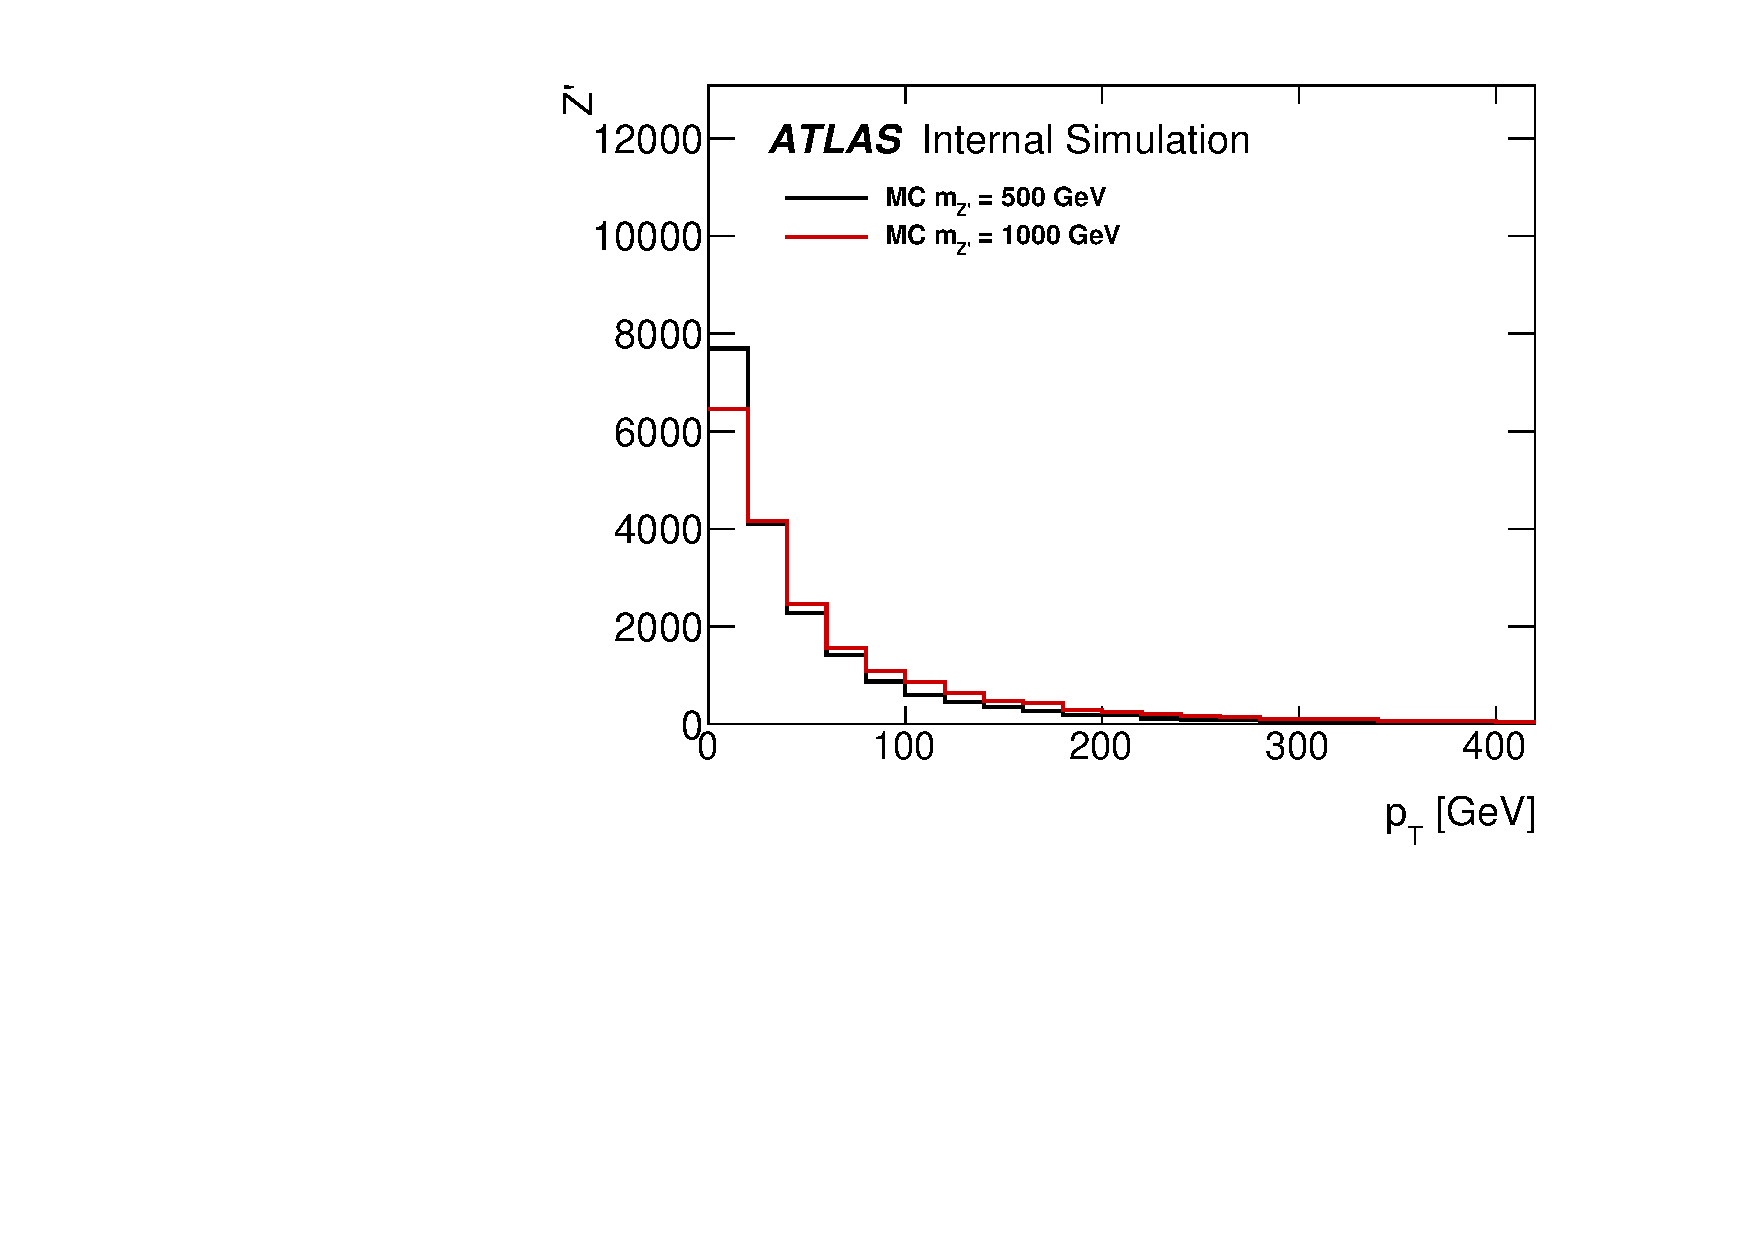
\includegraphics[width=0.45\textwidth]{figures/m_truth_zp_pt.pdf}}
    \subfloat[]{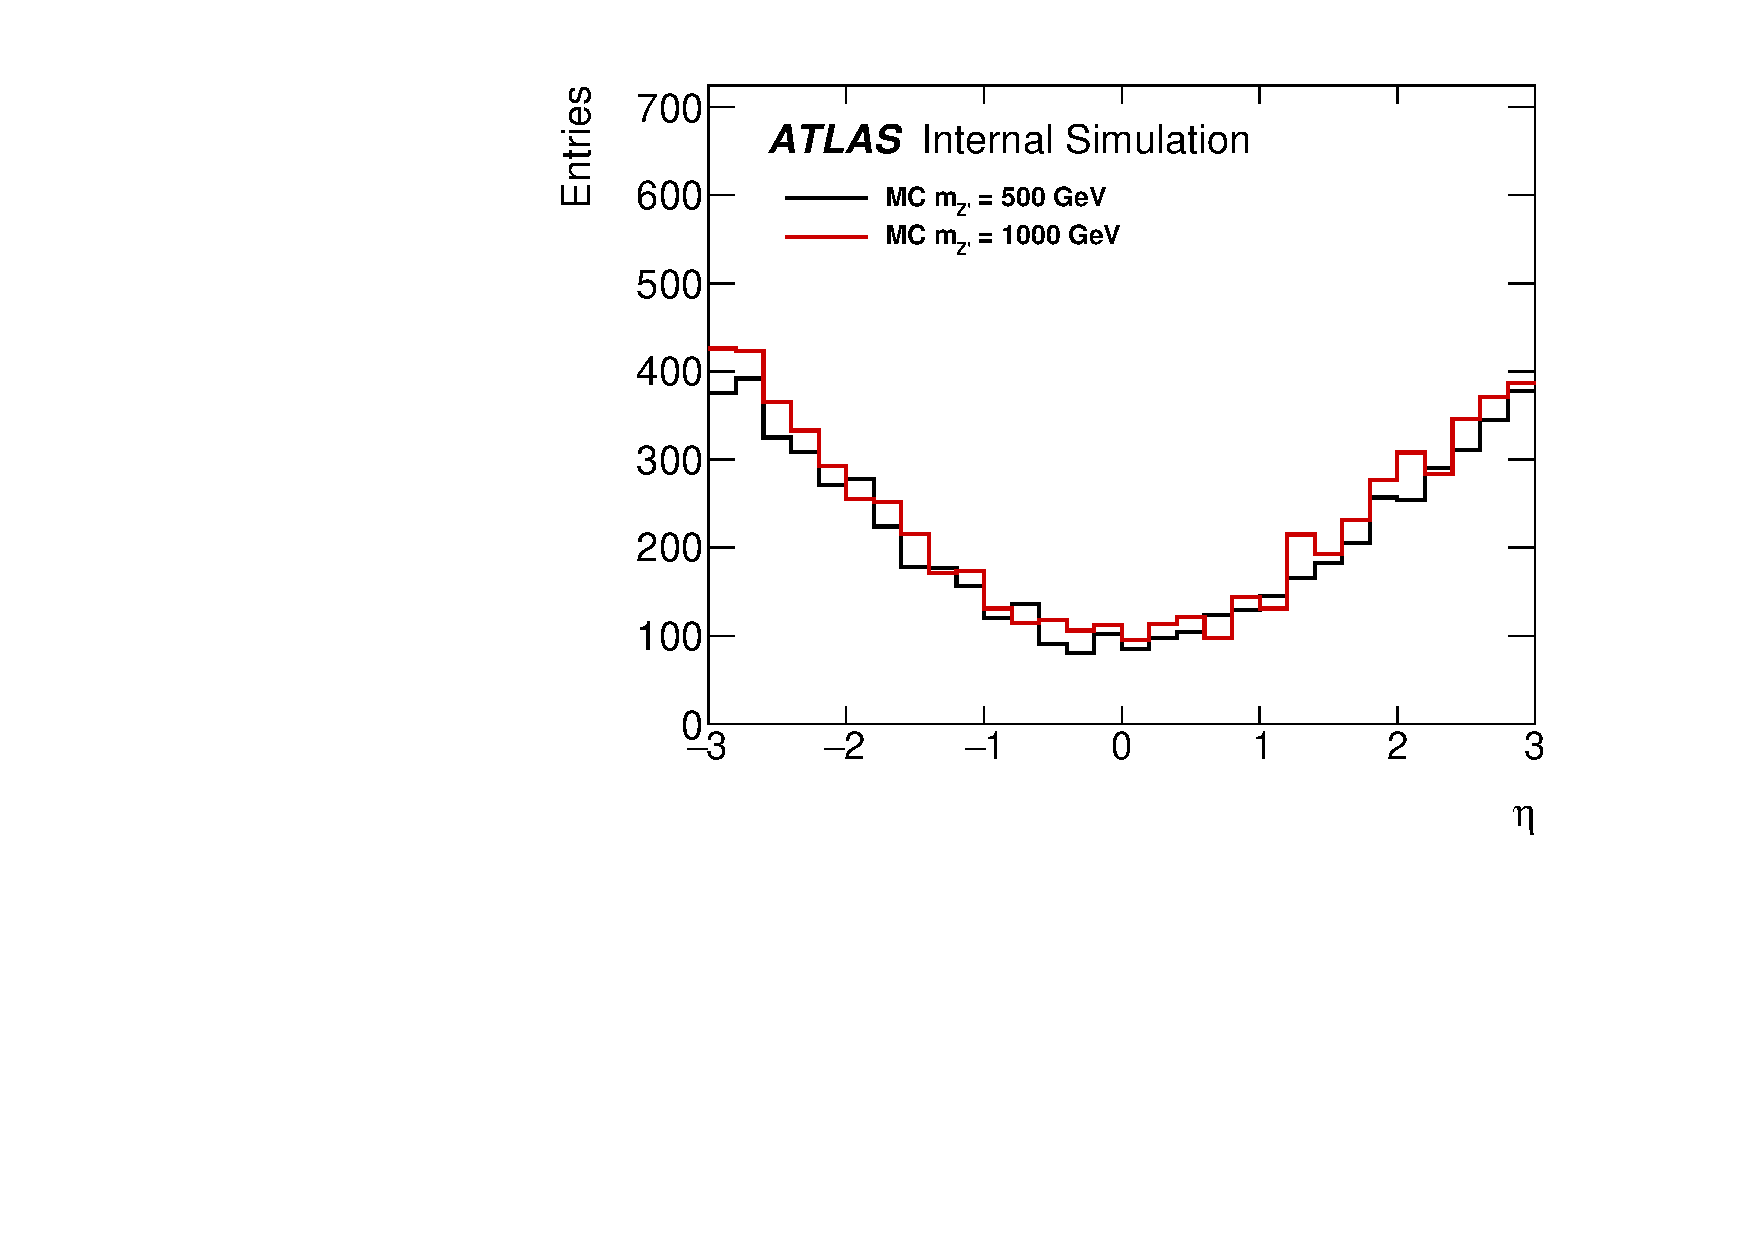
\includegraphics[width=0.45\textwidth]{figures/m_truth_zp_eta.pdf}} \\
    \subfloat[]{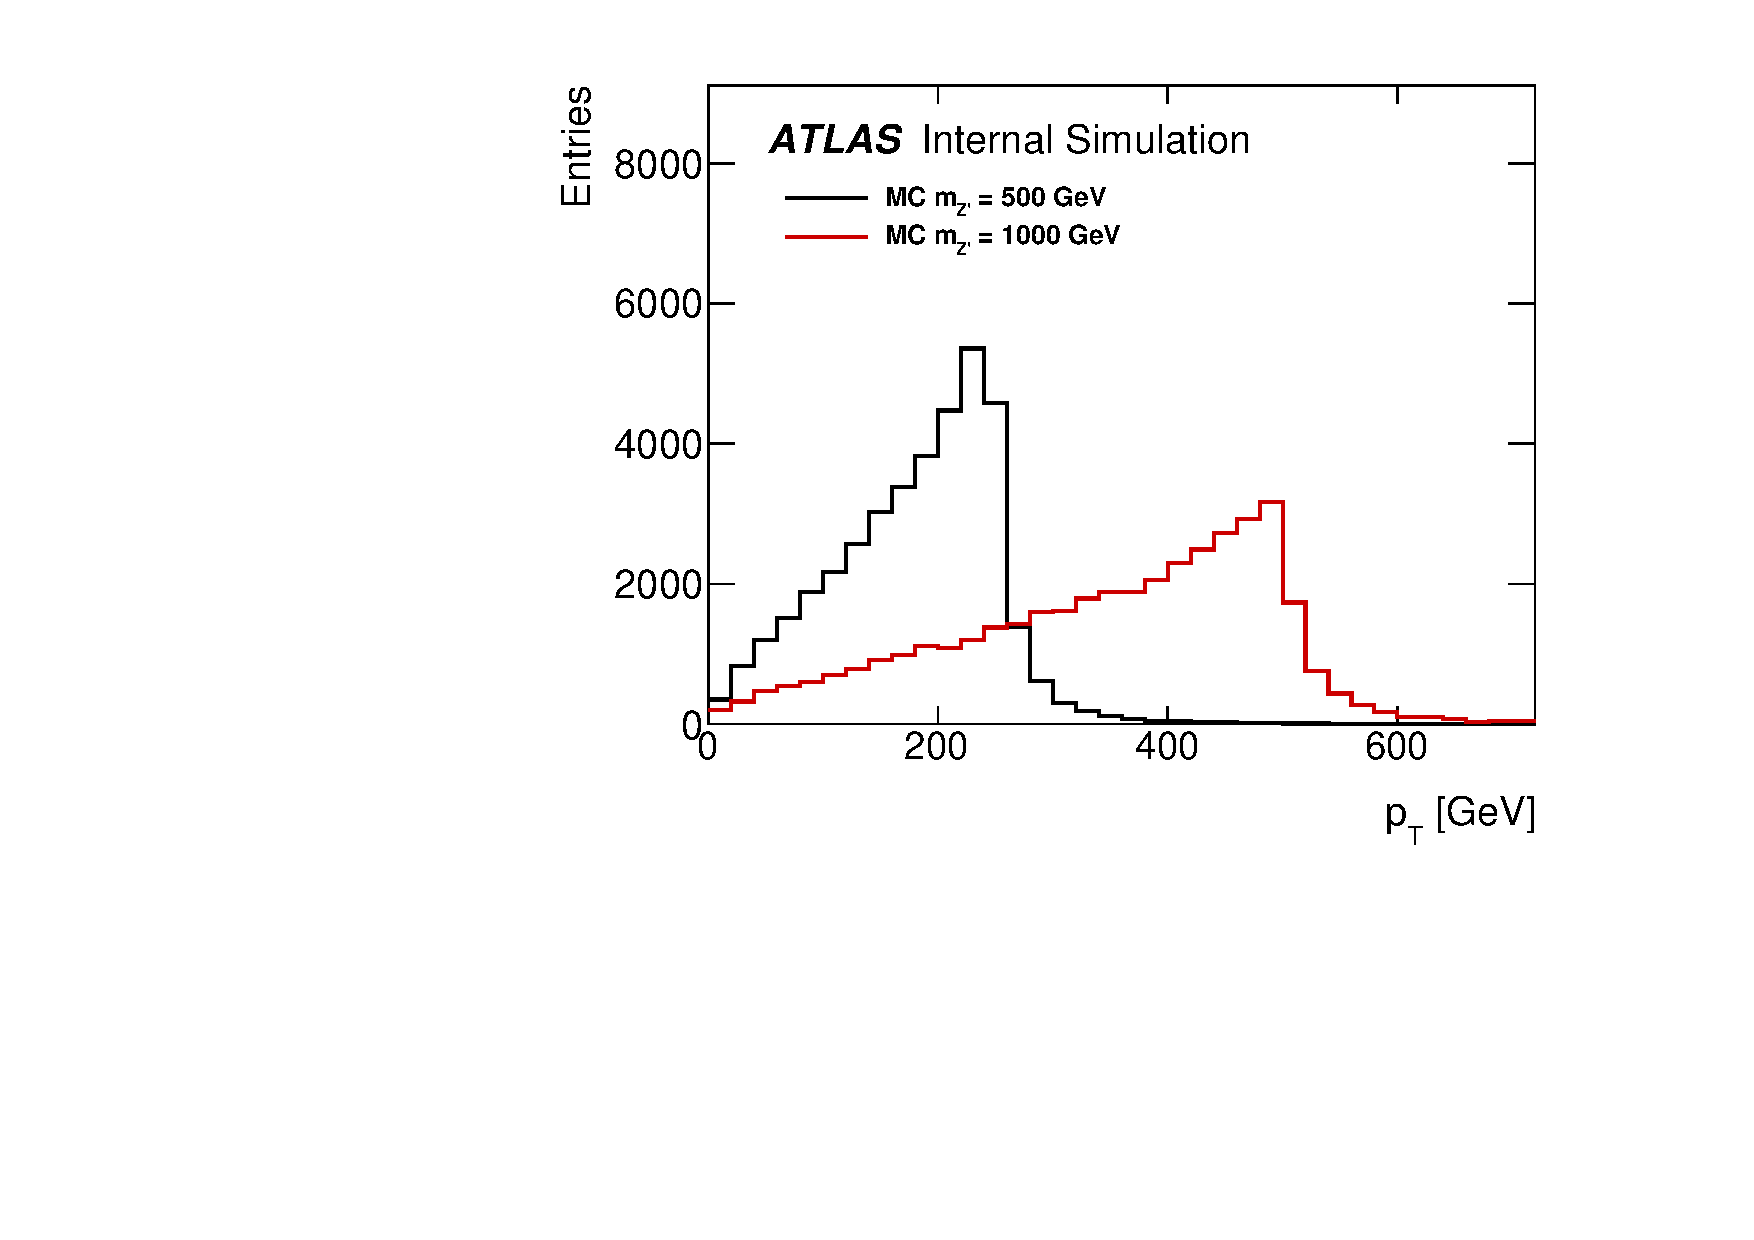
\includegraphics[width=0.45\textwidth]{figures/m_truth_muon_pt.pdf}}
    \subfloat[]{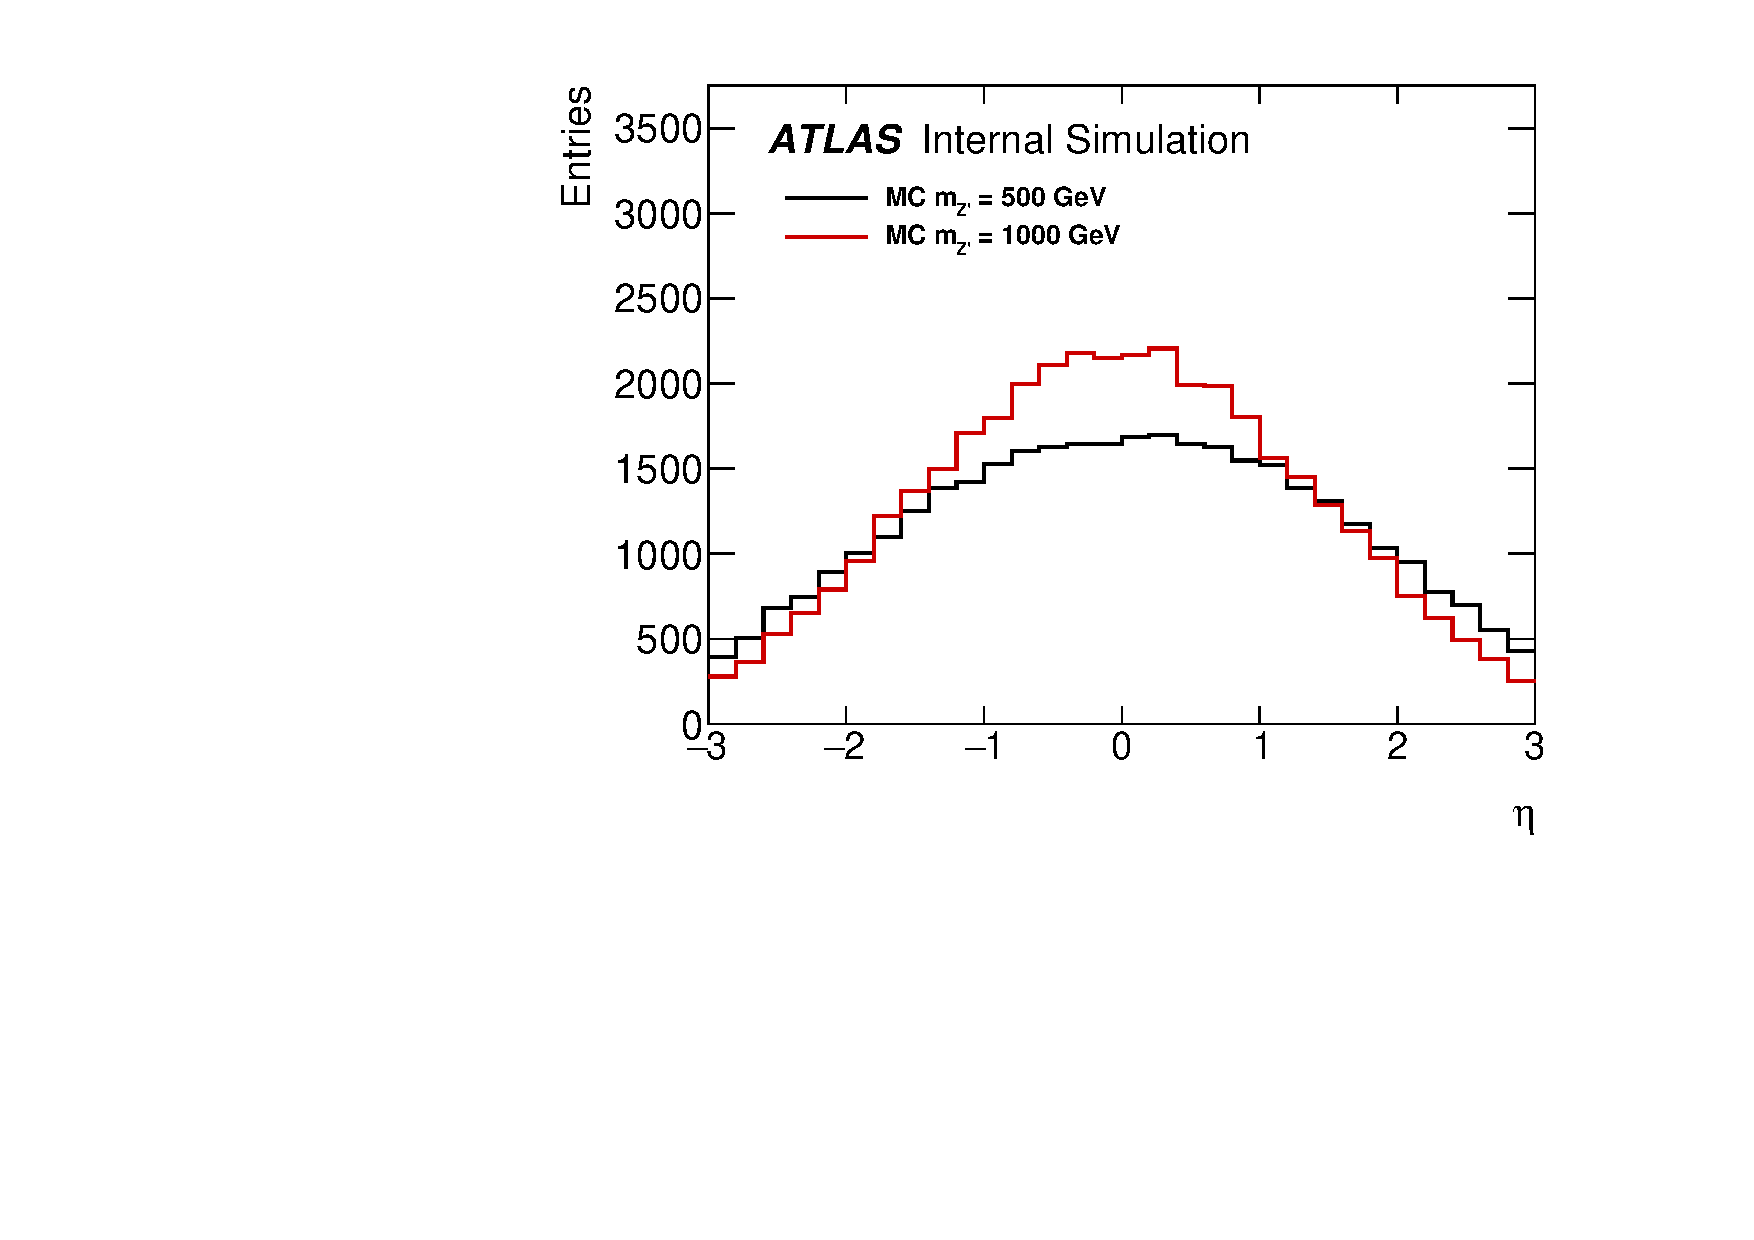
\includegraphics[width=0.45\textwidth]{figures/m_truth_muon_eta.pdf}}
    \caption{Representative plots of generator-level (a) $p_{T}$ and (b) $\eta$ distributions of $Z'$, and (c), (d) are the corresponding distributions for the signal muons. The signal MC samples are generated with $m=$ 500, 1000 GeV, and $c\tau=$ 100 mm.}
    \label{fig:truth_zp_muon}
\end{figure}


\subsection{Background MC Samples}
\label{sec:background_mc_sample}
In this analysis, backgrounds are estimated from data because most of the backgrounds are expected to originate from non-collision processes such as cosmic rays or random-crossing of tracks. %sources other than the SM collision process 

However, SM background samples are used to study the performance of random-crossing background estimation (Section~\ref{sec:bkg:random}) and to estimate the systematic uncertainties in vertexing and tracking (Section~\ref{sec:syst:vertexing}). The $t\bar{t}$ samples are generated for QCD background study using \sherpa 2.2~\cite{Gleisberg:2008ta} with the \texttt{NNPDF30NNLO} PDF set. The samples with leptonic decay of di-boson ($ZZ$, $WW$, $W^{\pm}Z$) are generated using \sherpa 2.1 with the \texttt{CT10} PDF set. The di-jet samples (JZ3W-JZ6W) are generated in slices of leading jet $p_{T}$ (160-400, 400-800, 800-1300, 1300-1800, 1800-2500 GeV) using \pythia 8.1 with \texttt{NNPDF23LO} PDF set. These samples are sufficient for testing purposes, as they contain high-$p_{T}$ isolated leptons (from $W$ boson decays) and leptons and displaced tracks in $b$-jets, in addition to tracks from pile-up vertices. Details on the PDF sets can be found in Ref.~\cite{Ball:2014uwa}.

The SM background samples are reprocessed using the same configuration as the signal MC sample for consistency. The background MC samples used for background and systematic uncertainty estimations are summarized in Table~\ref{table:background_MC}.


\begin{table}[!htb]
  \centering
  \begin{tabular}{ l l l l l}
    \hline
    \hline
    Process         &   DSID     &   $\sigma$ (pb)       & Events ($10^{6}$) &   $\mathcal{L}_{Int} (\mathrm{fb^{-1}})$ \\
    \hline
    $t\bar{t}$                              &   410252  &   87.8   &   0.70        &   7.97                 \\
    $ZZ\rightarrow \ell \ell \ell \ell$     &   361063  &   11.7   &   0.12        &   10.3                 \\
    $W^{-}Z\rightarrow \ell \ell \ell v$    &   361064  &   1.68   &   0.020       &   10.2                 \\
    $W^{+}Z\rightarrow \ell \ell \ell v$    &   361066  &   2.33   &   0.025       &   30.0                 \\
    $WW \rightarrow \ell \ell vv$           &   361068  &   12.8   &   0.13        &   1.95                 \\
    JZ3W                                    &   361023  &   8.45$\cdot10^{3}$      &   0.20  &   0.0247     \\
    JZ4W                                    &   361024  &   135    &   0.20        &   1.48                 \\
    JZ5W                                    &   361025  &   4.20   &   0.20        &   47.6                 \\
    JZ6W                                    &   361026  &   2.42$\cdot10^{-2}$     &   0.20  &   826        \\
    %$t\bar{t}$                              &   410252  &   76.3   &   0.70        &   9.17                 \\
    %$ZZ\rightarrow \ell \ell \ell \ell$     &   361063  &   12.8   &   0.12        &   9.30                 \\
    %$W^{-}Z\rightarrow \ell \ell \ell v$    &   361064  &   1.84   &   0.020       &   10.9                 \\
    %$W^{+}Z\rightarrow \ell \ell \ell v$    &   361066  &   2.56   &   0.025       &   9.77                 \\
    %$WW \rightarrow \ell \ell vv$           &   361068  &   14.0   &   0.13        &   9.29                 \\
    %JZ3W                                    &   361023  &   2.65$\cdot10^{7}$      &   0.20  &   < $10^{-5}$\\
    %JZ4W                                    &   361024  &   0.255  &   0.20        &   784                  \\
    %JZ5W                                    &   361025  &   0.455  &   0.20        &   440                  \\
    %JZ6W                                    &   361026  &   258    &   0.20  &   0.775      \\
    %JZ7W                                    &   361027  &   16.2                   &   0.10  &   0.617      \\
    \hline
    \hline
  \end{tabular}
  \caption{Background MC samples used in the study of random-crossing background and in the estimation of tracking and vertexing systematic uncertainty.}
  \label{table:background_MC}
\end{table}


Additional samples are used without the special reconstruction to study the efficiency of the triggers using tag-and-probe method (Section~\ref{sec:trigger_efficiency}). These samples are given in Table~\ref{table:background_MC:tag_probe}.

%\begin{table}[!htb]
\begin{sidewaystable}[!htb]
  \centering
  \resizebox{\textwidth}{!}{
    \begin{tabular}{ l l }
      \hline
      \hline
      Format     				& Dataset       													            \\
      \hline
      \texttt{DAOD\_EGAM1}	& mc15\_13TeV.361106.PowhegPythia8EvtGen\_AZNLOCTEQ6L1\_Zee.merge.DAOD\_EGAM1.e3601\_s2576\_s2132\_r7725\_r7676\_p3012  \\
      \texttt{DAOD\_MUON1}	& mc15\_13TeV.361107.PowhegPythia8EvtGen\_AZNLOCTEQ6L1\_Zmumu.merge.DAOD\_MUON1.e3601\_s2576\_s2132\_r7725\_r7676\_p3045	\\
      \hline
      \hline
    \end{tabular}
  }
  \caption{Background MC samples without the LRT used for tag and probe studies.}
  \label{table:background_MC:tag_probe}
%\end{table}
\end{sidewaystable}





\chapter{Signal Selection}
\label{chap:signal_selection}

The primary physics objects of this analysis are muons, electrons, and dilepton displaced vertices (DVs). In this section, the signal selection criteria for these physics objects are described.

\section{Event Preselection}
\label{sec:selection:pre}

Events are pre-selected in data processing using a combination of offline triggers and custom filters, called \texttt{DRAW\_RPVLL}. The selected events from the main physics stream are reprocessed for the special reconstruction. The filters are designed to select events containing displaced vertex candidates while maintaining reasonably low filter rates (< 30~\si{\hertz}). A single photon ($\gamma$), single electron ($e$), di-photon ($\gamma\gamma$), di-electron (\ee), and the combination of photon and electron ($e\gamma$) filters are used to select events with \ee or \emu candidates of interest. A single $\mu$ filter is used to select events with \mumu or \emu candidates of interest.

The filters require events to pass one of the HLTs listed in Table~\ref{table:triggers}. Most of the HLTs developed in ATLAS are designed for prompt searches, and there are implicit requirements on particles to point back to the IP. Therefore, the triggers with no requirement on ID tracks are used to increase the sensitivity to electrons and muons with large transverse and longitudinal impact parameters, $d_{0}$ and $z_{0}$. Consequently, the muon trigger that only uses the muon spectrometer information is used to trigger displaced muons. The photon triggers are used to trigger displaced electrons so that only the calorimeter information is used.

\begin{table}[!htb]
  \centering
  \begin{tabular}{l @{\hspace{1cm}} l}
    \hline
    \hline
    Description     			& Trigger	        	                \\
    \hline
	Single photon 	            & \texttt{HLT\_g140\_loose}             \\
	Di-photon	                & \texttt{HLT\_2g50\_loose}             \\
	Single muon                 & \texttt{HLT\_mu60\_0eta105\_msonly}   \\
    \hline
    \hline
  \end{tabular}
  \caption{HLTs used to select events in \texttt{DRAW\_RPVLL} filter. The single photon trigger requires one photon with $p_{T} > 140$ GeV. The di-photon trigger requires two photons with $p_{T} > 50$ GeV. The single muon trigger requires one muon with $p_{T} > 60$ within $|\eta| < 1.05$ using MS information only.}
  \label{table:triggers}
\end{table}

In addition to the HLT requirements, each filter requires offline selections on particles such as $p_{T}$, $\eta$, and $d_{0}$. The single photon ($\gamma$) or electron ($e$) filters require a leading photon or electron, respectively, with $p_{T} > 150$ GeV, $|\eta| < 2.5$, and $|d_{0}| > 2.0$ mm. These filters also require a second photon or lepton with $p_{T} > 10$ GeV and $|\eta| < 2.5$ to keep the filter rate reasonably low. The single muon $\mu$ filter requires a muon with $p_{T} > 60$ GeV, $|\eta| < 2.5$, and $|d_{0}| > 1.5$ mm. The di-photon ($\gamma\gamma$), di-electron (\ee), and the combination of photon and electron ($e\gamma$) filters require two photons/leptons with $p_{T} > 50$ GeV, $|\eta| < 2.5$, and $|d_{0}| > 2.0$ mm. The offline selection is summarized in Table~\ref{table:rpvll_filter_selection}.

\begin{table}[!htb]
  \centering
  \begin{tabular}{l c c c | c c c}
    \hline
    \hline
    Filter          & \multicolumn{3}{c|}{Leading}  &  \multicolumn{3}{c}{Secondary} \\
                    & $p_{T}$ (GeV) & $|\eta|$    & $|d_{0}|$ (mm) & $p_{T}$ (GeV) & $|\eta|$    & $|d_{0}|$ (mm)  \\
    \hline
    $\gamma$, $e$                   & $>$ 150   & $<$ 2.5  & $>$ 2.0  & $>$ 10 & $<$ 2.5 & -       \\
    $\mu$                           & $>$ 62    & $<$ 2.5  & $>$ 1.5  & -      & -      & -       \\
    $\gamma\gamma$, \ee, $e\gamma$ & $>$ 55    & $<$ 2.5  & $>$ 2.0  & $>$ 55 & $<$ 2.5 & $>$ 2.0 \\
    \hline
    \hline
  \end{tabular}
  \caption{\texttt{RPVLL} filter offline selection on photon and leptons.}
  \label{table:rpvll_filter_selection}
\end{table}

The events selected by the \texttt{RPVLL} filters are passed downstream for the special reconstruction process, and the physics objects such as electron, muon, and secondary vertices are reconstructed for analysis.




\subsection{Event Selection}
\label{sec:event_selection}
%Events are selected by minimum requirements on the quality of events, completeness of luminosity blocks, and HLTs used in this analysis. The event selections are as follows.
At analysis-level, minimum requirements are placed on events based on the quality of events, completeness of the corresponding luminosity blocks, primary vertex, and HLTs used in this analysis. In addition, a cosmic veto is applied to reject events with back-to-back muons. The event selection is described below:

\begin{itemize}
    \item \texttt{GoodRunsList} removes events from incomplete luminosity blocks.
    \item Event cleaning removes corrupted/bad events due to problems in TileCal, LAr calorimeter noise bursts, and detector downtimes.
    \item Events are required to pass one of the HLTs listed in Table~\ref{table:triggers}.
    \item At least one primary vertex is required along the beam line ($|z|<200$ \si{\mm}).
    \item Events are rejected if there is a pair of leptons with $\Rcr = \sqrt{(\Delta \phi - \pi)^{2} + (\Sigma \eta)^{2}} < 0.01$.
\end{itemize}

%The event selection is summarized in Table~\ref{table:signal_selection}.


\subsection{Muon and Electron Requirements}
\label{sec:muon_electron_selection}

The analysis searches for displaced vertices with two leptonic tracks, \mumu, \ee, and \emu. Prior to applying the vertex level selections, tracks from vertices are required pass muon or electron selections based on track quality, kinematics, and lepton identification criteria. 

Electron requirements are based on the recommendations from the Electron-Gamma (EG) group with an optimization for electrons with large impact parameters. Electrons are rejected if there is a bad cluster associated with an electron. Basic kinematic cuts are applied to electrons, $|\eta| < 2.47$ and $p_{T}$ > 10 GeV. The EG group provides several electron identification criteria, called working points, based on a likelihood discriminant to suppress background electrons originating from photon conversions and heavy flavour decays. In this analysis, the electron \texttt{LooseLH} working point is used, but the requirements on $d_{0}$ and silicon hits are removed to improve electron detection efficiency at large impact parameters.

Muon requirements are based on the recommendations from the Muon Combined Performance group with similar optimizations as electrons. The muon \texttt{Loose} working point is used for the identification criteria, and a fiducial cut, $|\eta| < 2.5$, and kinematic cut, $p_{T}$ > 10 GeV, are applied to muons. The requirements on Pixel hits are removed to improve muon detection efficiency at large impact parameter. Muons are required to have an associated ID track for vertex reconstruction. In the case of MC samples, muon momentum resolution and scale corrections are applied to the simulated muons for better agreement between data and simulation~\cite{Aad:2016jkr}.

Overlap removal is applied to both muons and electrons to ensure that a ID track is associated with only one muon or electron. The muon and electron requirements are summarized in Table~\ref{table:lepton_requirement}.

\begin{table}[!htb]
  \centering
  \begin{tabular}{ l  l }
    \hline
    \hline
    \textbf{Muon}     &       Overlap removal                                                                      \\
                                  &       Muon \texttt{Loose} (no requirement on Pixel hits)                       \\
                                  &       $|\eta| < 2.5$                                                           \\
                                  &       $p_{T} > 10$ GeV                                                         \\
                                 % &       Associated Inner detector track                                          \\
                                  &       Combined Muon                                                            \\
    \hline
    \textbf{Electron} &       Overlap removal                                                                      \\
                                  &       Bad cluster removal                                                      \\
                                  &       Electron \texttt{LooseLH} (no requirement related to $d_{0}$, silicon hits)\\
                                  &       $|\eta| < 2.47$                                                          \\
                                  &       $p_{T} > 10$ GeV                                                         \\
    \hline
    \hline
  \end{tabular}
  \caption{Muon and electron requirements applied at analysis level.}
  \label{table:lepton_requirement}
\end{table}







\subsection{Vertex Selection}
\label{sec:vertex_selection}
The vertex selection is applied to two-track secondary vertices found in Section~\ref{sec:reco:dv}. Secondary vertices with displacement of $r_{\mathrm{DV}}>$ 2 mm from the primary vertex are selected. The selected displaced vertices are made of two tracks which can be any combination of muon, electron, and non-lepton tracks. Therefore, vertices are separated into three vertex types, control, validation, and signal regions.

In the control region, vertices are required to have two non-leptonic tracks (\xx). In the validation region, vertices are required to have a muon or an electron and another non-leptonic track (\mux, \ex). In signal region, vertices are required to have a muon pair, an electron pair, or a muon-electron pair (\mumu, \ee, \emu). The control region and the validation region are used for background (Chapter~\ref{chap:bkg}) and systematic uncertainty (Section~\ref{chap:syst}) estimations. The control, validation, and signal regions are summarized in Table~\ref{table:vertex_type}.

\begin{table}[!h]
  \centering
  \begin{tabular}{ l @{\hspace{1cm}} c}
    \hline
    \hline
	Region				& Vertex Type										\\
    \hline
	Control     		& \xx   										\\
	Validation       	& \mux, \ex										\\
	Signal       		& \mumu, \ee, \emu							\\
    \hline
    \hline
  \end{tabular}
  \caption{The control, validation, and signal regions defined by the vertex type.}
  \label{table:vertex_type}
\end{table}

In all regions, vertices are required to pass a common set of vertex selections described as follows. Vertices are required to have $\chi^2 / \mathrm{ DOF} <$ 5, which is the default selection used by the Tracking Combined Performance group, to reject poorly reconstructed vertices. A minimum transverse displacement of 2~\si{mm} from the primary vertex is required to suppress background from prompt decays. Two tracks from a vertex are required to have opposite electric charges. Vertices within the volume of disabled Pixel module~\cite{Backhaus:2110260} are rejected. Since hadronic interactions of charged particles with detector material produces irreducible backgrounds, the vertices within dense detector material~\cite{Aaboud:2215485} are rejected. The material veto is not applied to \mumu vertex due to low probability of muon interaction with detector material. Vertices are also required to be in the detector volume covered by the material mapping ($r < 300$~\si{mm}, $|z| < 300$~\si{mm}). The invariant mass of the lepton pairs, also referred as vertex mass, is required to have $m_{\ell\ell} >$ 10 GeV to suppress backgrounds from low mass SM particles such as $J/\Psi$ and $\Upsilon$. The vertex mass is calculated by the secondary vertex reconstruction algorithm with the assumption that all tracks are pions. A cosmic veto is applied to vertices by requiring $\Rcr > 0.01$. The veto is very effective in rejecting cosmic muons reconstructed as back-to-back muon vertices, and the details are discussed in Section~\ref{sec:bkg:cosmic}.

In addition to the common vertex selection, at least one electron or muon from the vertex is required to match one of the HLTs listed on Table~\ref{table:triggers} and the filters listed on Table~\ref{table:rpvll_filter_selection} in the signal region. The vertex selection is summarized in Table~\ref{table:signal_selection}.

\begin{table}[!htb]
  \centering
  \begin{tabular}{ l @{\hspace{1cm}} l }
    \hline
    \hline
    \textbf{Event}           &       GoodRunsList                                                                \\
                             &       Event cleaning                                                              \\
                             &       Trigger filter                                                              \\
                             &       Cosmic veto                                                                 \\
                             &       Primary vertex ($|z|<$200~\si{\mm})                                         \\
    \hline
    \textbf{Vertex}          &       Trigger matching (signal region only)                                       \\
                             &       $\chi^2 / \mathrm{ DOF} < 5$                                                \\
                             &       $r_{\mathrm{DV}} > $ 2 mm                                                            \\
                             &       Opposite charge                                                             \\
                             &       Disabled module veto                                                        \\
                             &       Material veto (excluding \mumu)                                             \\
                             &       $m > 10$ GeV                                                                \\
                             &       $r < 300$~\si{mm}, $|z| < 300$~\si{mm}                                      \\
                             &       Filter matching (signal region only)                                                            \\
    \hline
    \hline
  \end{tabular}
  \caption{Event and vertex selections applied to select displaced vertices.}
  \label{table:signal_selection}
\end{table}


\chapter{Signal Efficiency}
\label{chap:eff}

A signal efficiency of finding displaced dilepton vertex is defined by the ratio of the number of events passing the signal selection (Chapter~\ref{chap:signal_selection}) to the total number of events generated. The signal efficiency can be written as Eq.~\ref{eq:OverallEff}. 

\begin{equation}
\label{eq:OverallEff}
\varepsilon_{\mathrm{overall}} = \varepsilon_{\mathrm{filter}} \cdot \varepsilon_{\mathrm{trigger}} \cdot 
                     (\varepsilon_{\mathrm{tracking}} \cdot \varepsilon_{\mathrm{lepton}})^2 \cdot
                     (\varepsilon_{\mathrm{vertexTrack}})^2 \cdot
                     \varepsilon_{\mathrm{vertexFit}}.
\end{equation}
%
$\varepsilon_{\mathrm{filter}}$ and $\varepsilon_{\mathrm{trigger}}$ together represent the efficiency of \texttt{RPVLL} filter, the ratio of the events passing \texttt{RPVLL} filter to the total events processed. \texttt{RPVLL} filter has the trigger filter as one of its requirements. Because it is desirable to study the trigger efficiency independently from the filter efficiency, \texttt{RPVLL} filter efficiency is factorized into the filter efficiency and the trigger efficiency. $\varepsilon_{\mathrm{tracking}}$ represents the efficiency to reconstruct ID tracks from signal particles, and $\varepsilon_{\mathrm{lepton}}$ represents the efficiency to reconstruct and identify the signal particles as leptons using ID tracks, energy deposite in calorimeters, and MS tracks. $\varepsilon_{\mathrm{vertexTrack}}$ represents the efficiency for the reconstructed signal leptons to be selected for secondary vertex reconstruction, and $\varepsilon_{\mathrm{vertexFit}}$ represents the efficiency to reconstruct a displaced vertex using two signal leptons and pass the vertex selection.
%Therefore, $\varepsilon_{\mathrm{filter}}$ is defined by the fraction of events passing \texttt{RPVLL} filter requirements without the trigger filter, and $\varepsilon_{\mathrm{trigger}}$ is defined by the fraction of events passing one of the HLTs used in this search.

In order to understand the source of signal efficiency loss, the trigger efficiency is studied in Section~\ref{sec:trigger_efficiency}, and the tracking and lepton identification efficiencies are studied in Section~\ref{sec:tracking_efficiency}. In Section~\ref{sec:combined_reco_efficiency}, the overall reconstruction efficiency, also referred as signal efficiency, of the $Z'$ signal model after the full analysis selection is presented. 

\section{Trigger efficiency}
\label{sec:trigger_efficiency}
The trigger efficiency is defined as the ratio of the events passing one of the triggers used in this analysis to the total events generated. In this analysis, three triggers listed on Table~\ref{table:triggers} are used to select the events with displaced dilepton vertex candidates. The single muon trigger is sensitive to the events with a \mumu or \emu vertex. The di-photon trigger is mainly used to select the events with an \ee vertex, but a small number of events with an \emu vertex pass this trigger. The single photon trigger is sensitive to events with \ee or \emu vertex, but its efficiency is relatively low in comparison with the other two triggers.

To illustrate the impact of the trigger efficiencies on the signal samples, the efficiency of each trigger and the combined trigger efficiency is shown in Figure~\ref{fig:m_trig_eff_allchannel} using the signal MC samples of $Z'$ decaying to all three channels at $m = $ 250 GeV and $c\tau=$ 250 mm. The sample with \ee channel shows the highest combined trigger efficiency due to the high efficiency in di-photon trigger, and the sample with \emu channel shows the reduced combined trigger efficiency because \emu vertices have only one track that can satisfy either the single muon or photon trigger.

\begin{figure}[!htb]
	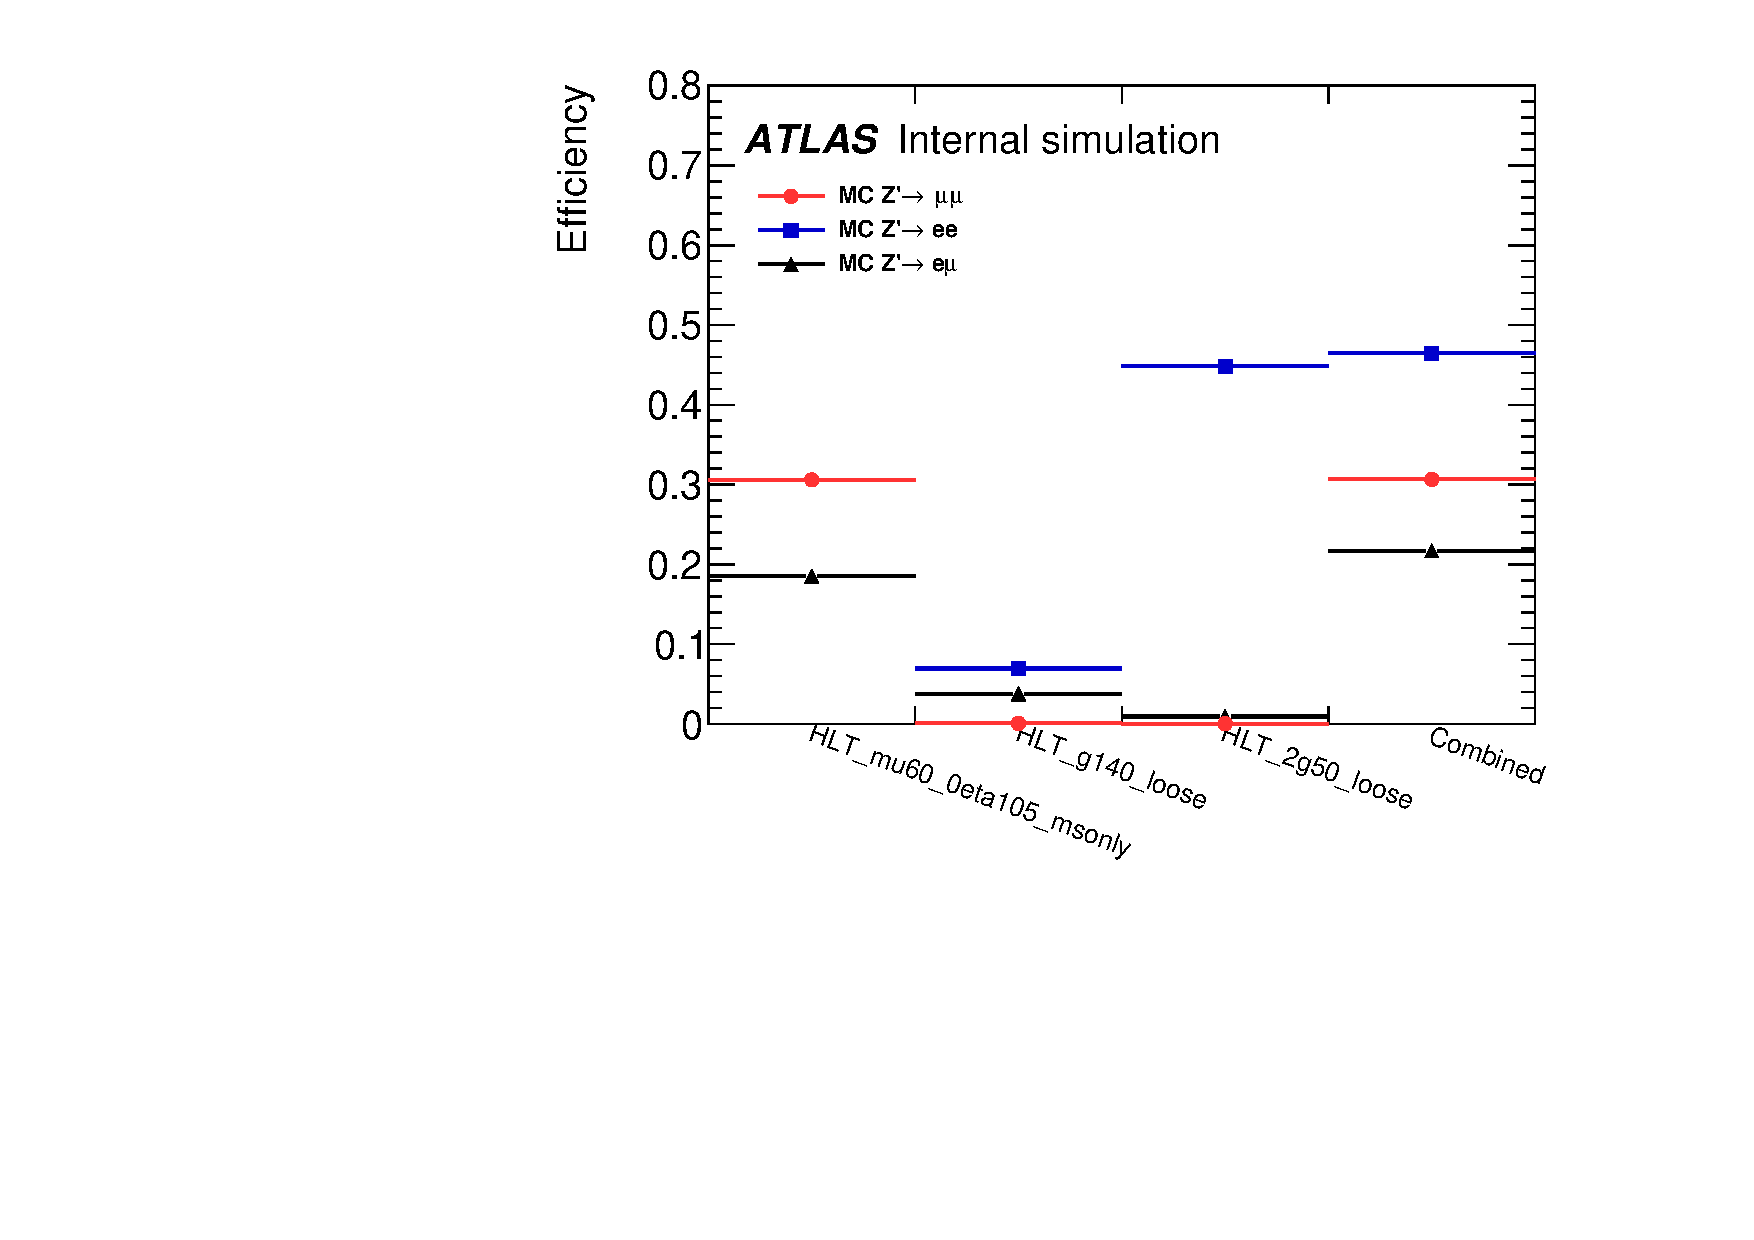
\includegraphics[width=0.60\textwidth]{figures/m_dv_eff_trig_allchannel.pdf}
	\centering
	\caption{Trigger efficiency of single muon, single photon, di-photon, and the combined triggers of the signal MC samples of $Z'\rightarrow\mumu, \ee$, and \emu generated with $m=$ 250 GeV and $c\tau=$ 250 mm.}
	\label{fig:m_trig_eff_allchannel}
\end{figure}

The trigger efficiency on all \mumu signal MC samples is shown in Table~\ref{table:m_trig_eff_mumu}. It is evident that at low $Z'$ mass ($\sim$100 GeV), the combined trigger efficiency on the signal MC sample is significantly reduced because the typical $p_{T}$ of the signal muons is lower than the $p_{T}$ threshold of the single muon trigger.

The trigger study indicates that there is a substantial loss in the signal efficiency at trigger level before reconstruction, and developing dedicated, more efficient triggers for long-lived particles will provide potential improvement in sensitivity to long-lived particles. The systematic uncertainties in trigger efficiency is estimated by tag-and-probe method in Section~\ref{sec:syst:trigger}.

\begin{table}[!htb]
  \centering
  \begin{tabular}{ c c | c c c c}
    \hline
    \hline
    %       &       & \multicolumn{4}{c}{$Z'\rightarrow\mumu$}                \\
    $m_{Z'}$ (GeV) & $c\tau$ (mm) & Single muon & Single photon & Di-photon & Combined \\
    \hline
    100			&	100	& 0.047 	& < 0.001   &0  	    &0.047  		\\
    100			&	250	& 0.043  	&0  	 	&0  	    &0.043  		\\
    100			&	500	& 0.039 	&0  	 	&0  	    &0.039  		\\
    250			&	100	& 0.343  	&< 0.001 	&< 0.001    &0.344  		\\
    250			&	250	& 0.306  	&< 0.001 	&< 0.001    &0.307  		\\
    250			&	500	& 0.230 	&< 0.001 	&< 0.001    &0.230  		\\
    500			&	100	& 0.454 	&0.010   	&< 0.001    &0.459  		\\
    500			&	250	& 0.410 	&0.009   	&< 0.001    &0.415  		\\
    500			&	500	& 0.331  	&0.008   	&0.001      &0.336  		\\
    750			&	100	& 0.541 	&0.026   	&0.002      &0.553  		\\
    750			&	250	& 0.470 	&0.023   	&0.003      &0.481  		\\
    750			&	500	& 0.391 	&0.022 	    &0.001      &0.402  		\\
    1000	    &	100	& 0.570   	&0.039   	&0.004      &0.586  		\\
    1000	    &	250	& 0.512   	&0.036   	&0.003      &0.526  		\\
    1000	    &	500	& 0.430   	&0.034 	    &0.004      &0.444  		\\
    \hline
    \hline
  \end{tabular}
  \caption{Trigger efficiency of single muon, single photon, di-photon triggers, and the combined trigger efficiency on the signal MC samples of $Z'\rightarrow\mumu$.}
  \label{table:m_trig_eff_mumu}
\end{table}

\section{Lepton reconstruction efficiency}
\label{sec:tracking_efficiency}
The tracking efficiency, $\varepsilon_{\mathrm{track}}$, and the lepton identification efficiency, $\varepsilon_{\mathrm{lepton}}$, are studied together as a lepton reconstruction efficiency. The lepton reconstruction efficiency is defined and estimated as follows. From a signal MC sample, the leptons decaying from $Z'$ are collected at generator-level, referred as \textit{truth} signal leptons. For each truth signal lepton, if there is a reconstructed lepton with its ID track matched to the ID track of the truth signal lepton by a hit-based truth matching scheme, it is marked as reconstructed. The ratio of reconstructed signal leptons to the total number of signal leptons produced in the sample is taken as the lepton reconstruction efficiency. No \texttt{RPVLL} or trigger filter is applied in estimating the lepton reconstruction efficiency.

Figure~\ref{fig:lepton_eff} shows the representative plot of the lepton reconstruction efficiency as a function of track parameters using the combined signal MC samples of $Z'$ decaying to all three channels, generated with $m = $ 250 GeV and $c\tau=$ 250 mm.

\begin{figure}[!htb]
    \centering
    \subfloat[]{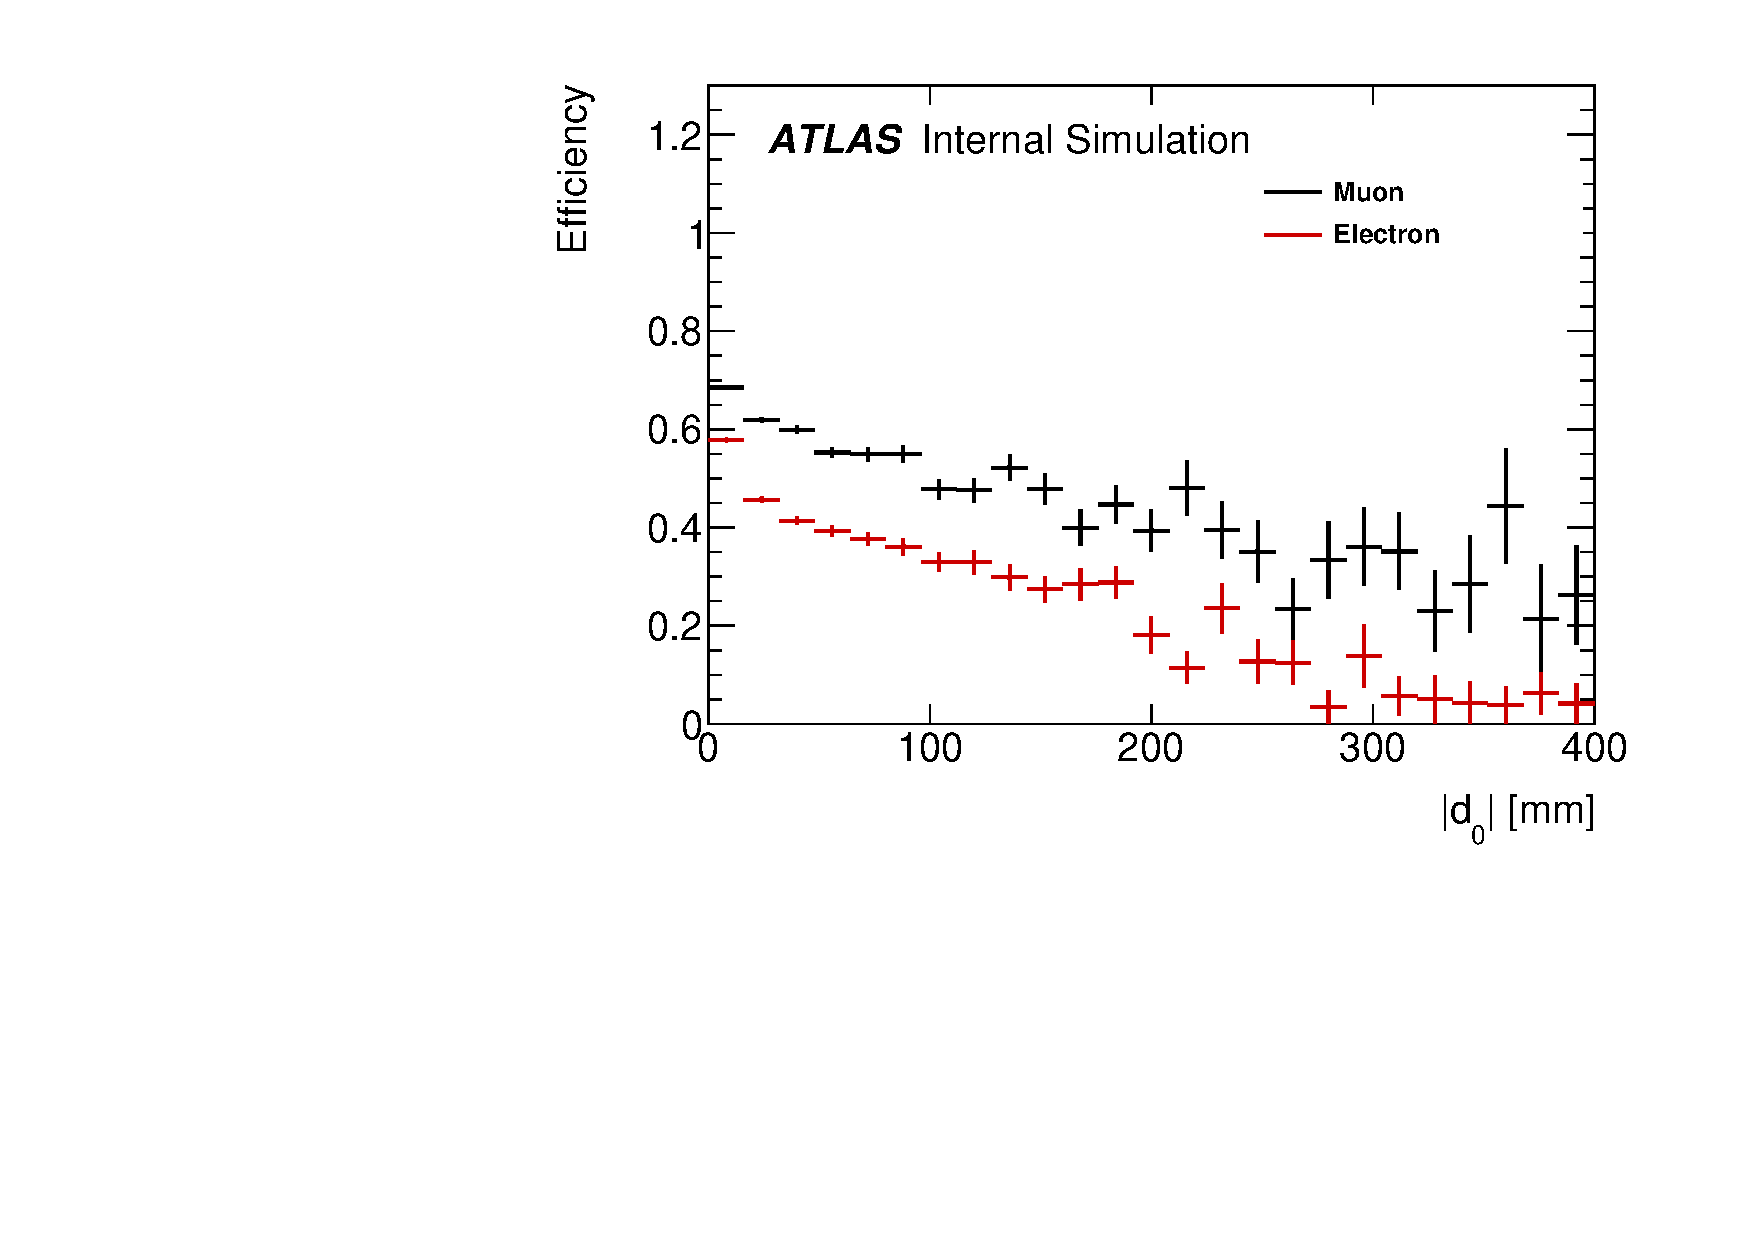
\includegraphics[width=0.50\textwidth]{figures/m_lepton_efficiency_d0.pdf}}
    \subfloat[]{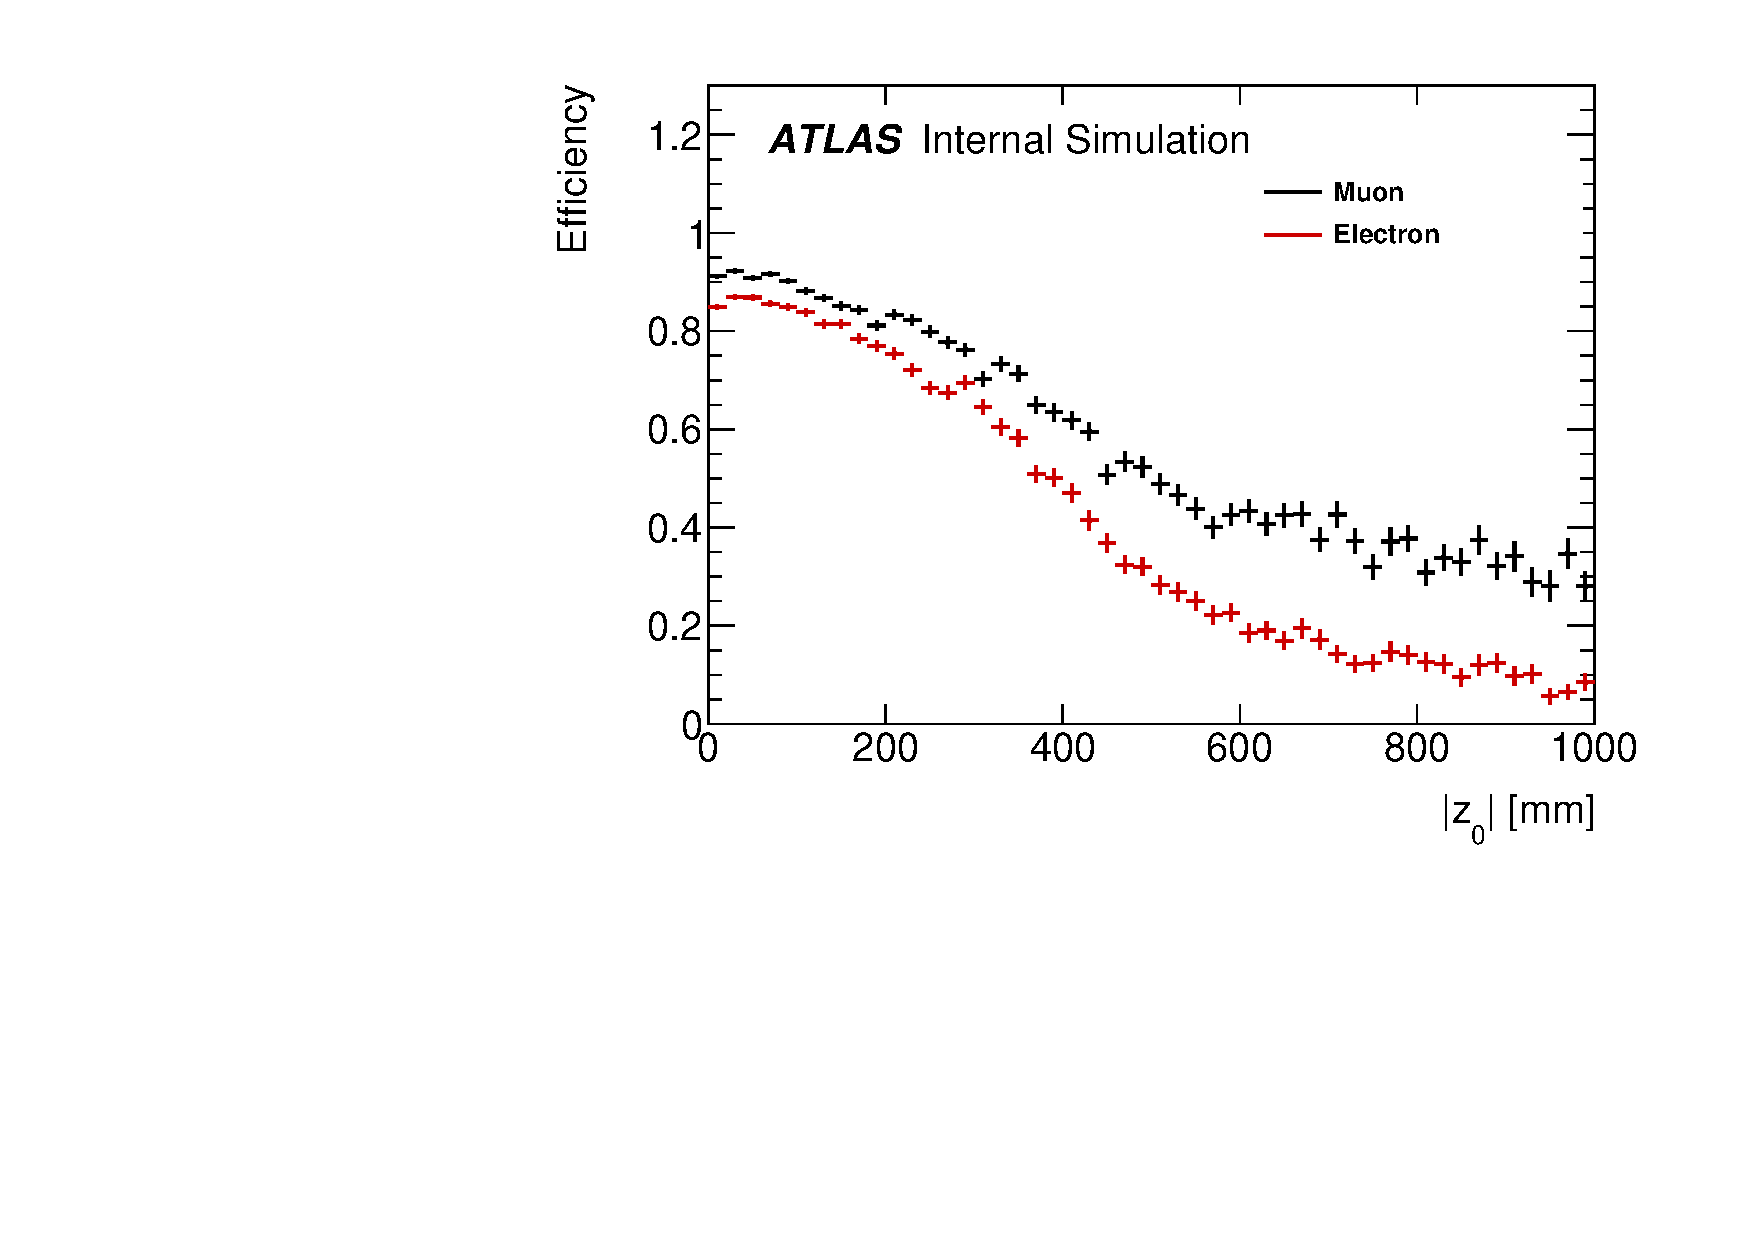
\includegraphics[width=0.50\textwidth]{figures/m_lepton_efficiency_z0.pdf}} \\
    \subfloat[]{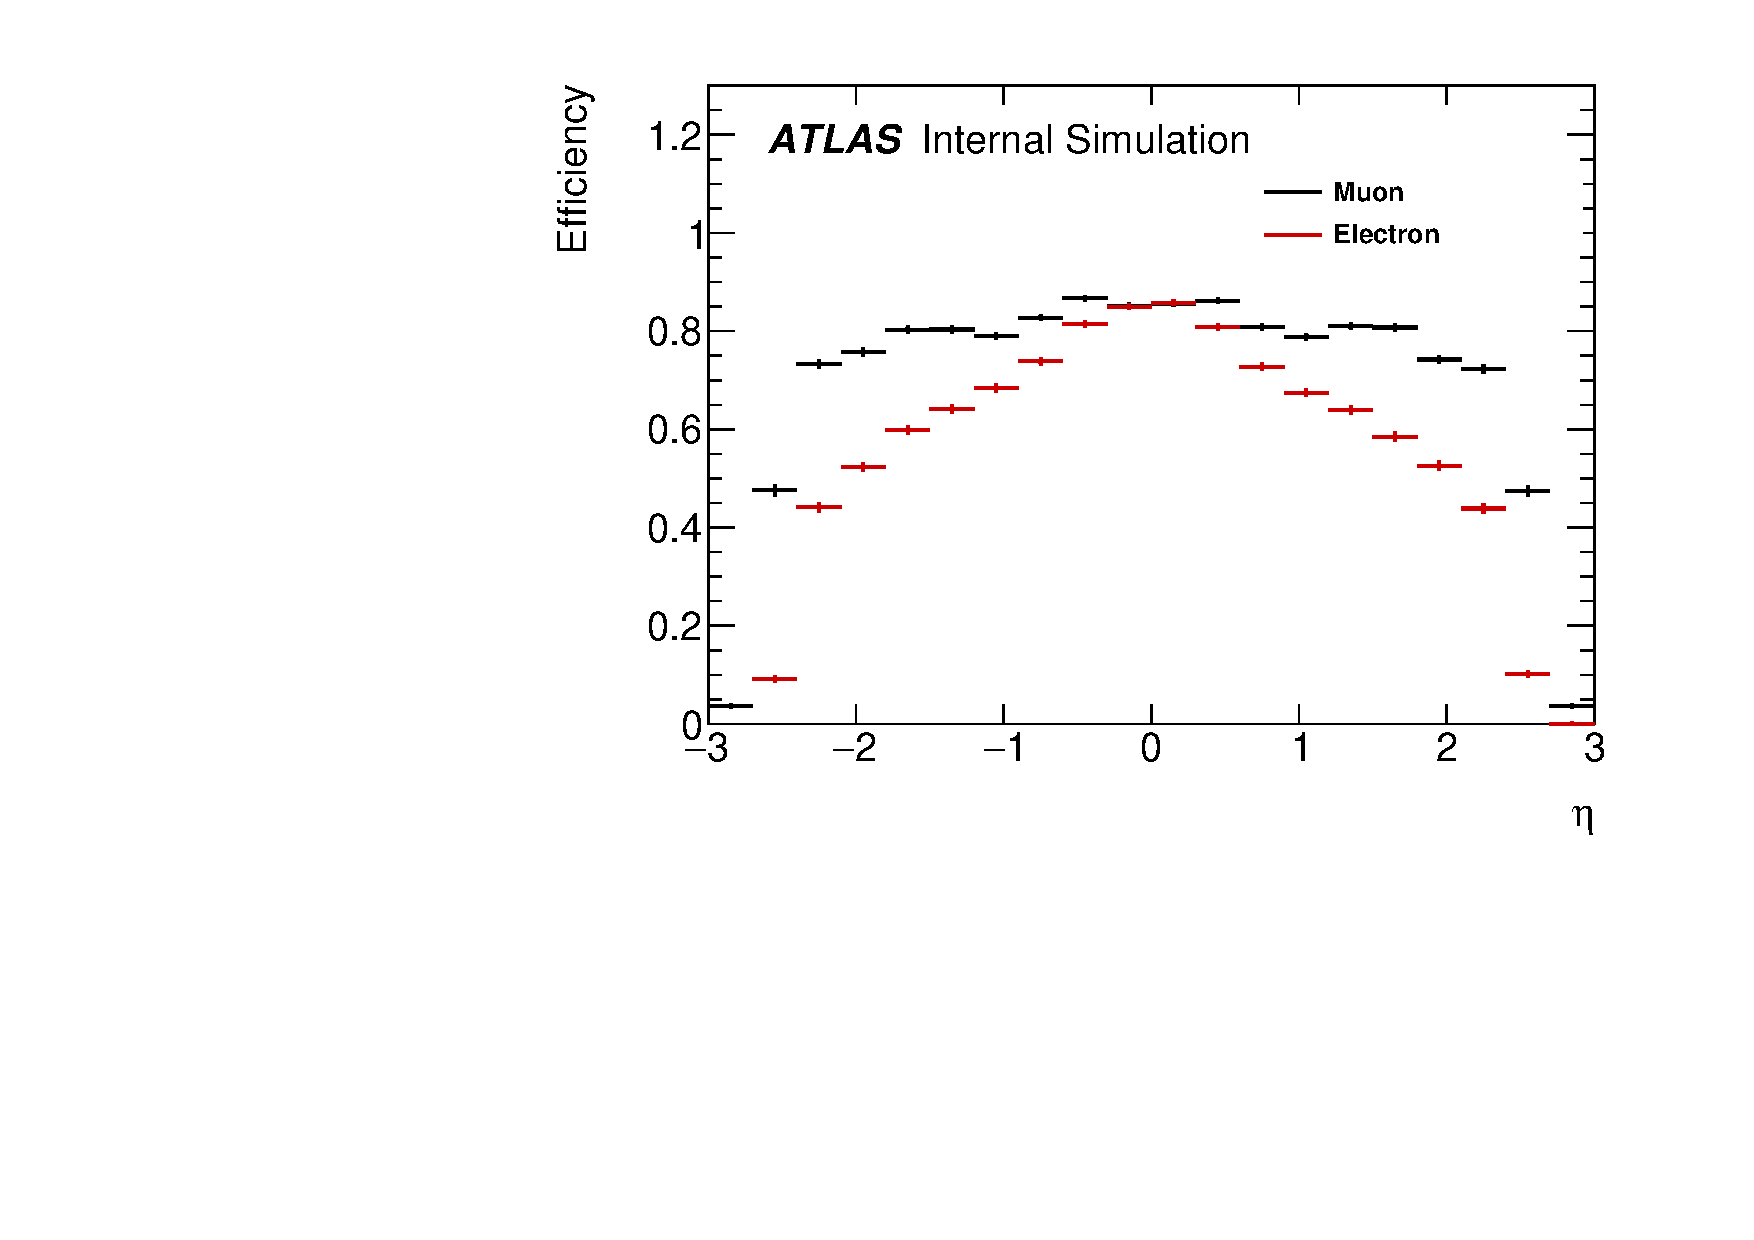
\includegraphics[width=0.50\textwidth]{figures/m_lepton_efficiency_eta.pdf}}
    \subfloat[]{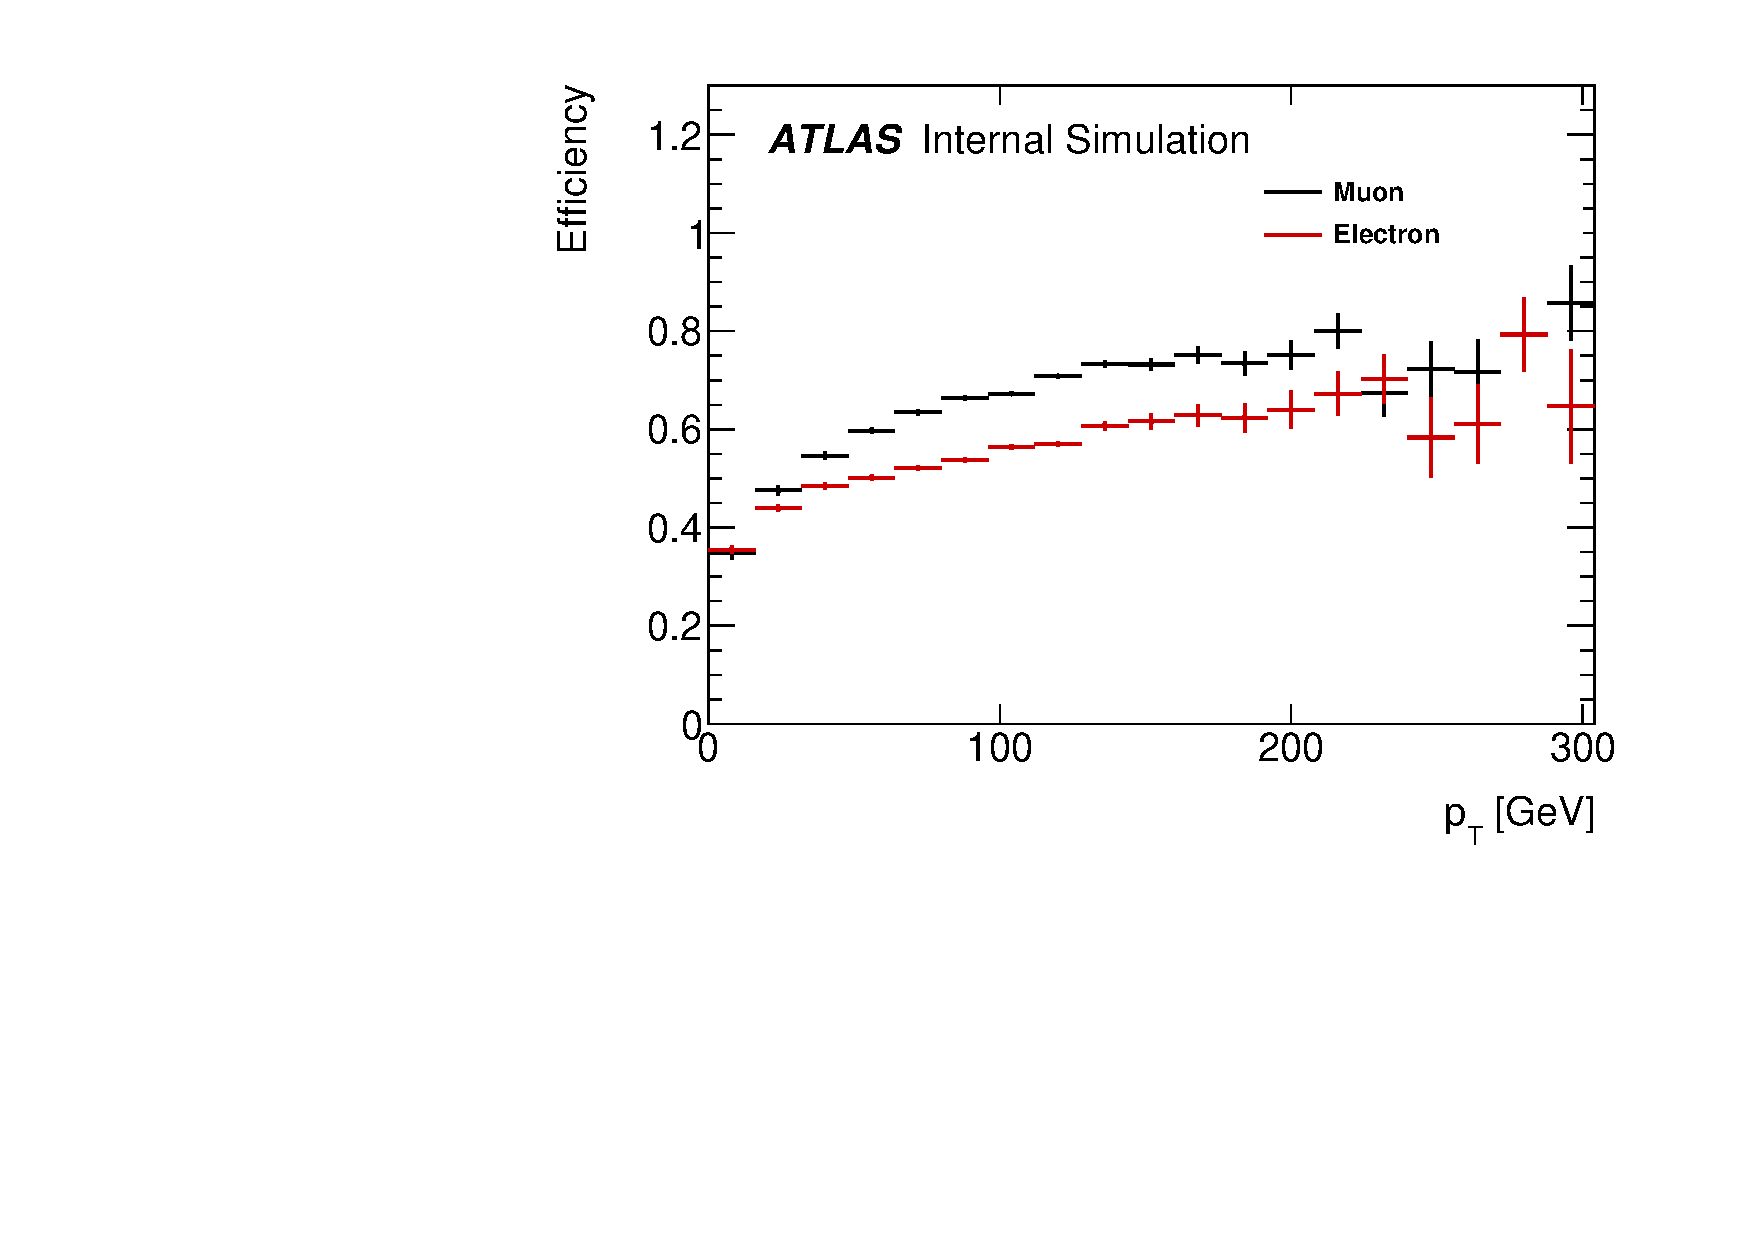
\includegraphics[width=0.50\textwidth]{figures/m_lepton_efficiency_pt.pdf}} 
    \caption{Lepton reconstruction efficiency as a function of (a) $d_{0}$, (b) $z_{0}$, (c) $\eta$, and (d) $p_{T}$ of signal leptons using the signal MC sample generated with $m=$ 250 GeV and $c\tau=$ 250 mm.}
    \label{fig:lepton_eff}
\end{figure}

It is evident that the efficiency drops drastically at $\eta > 2.0$ where the Pixel barrel region ends due to the minimum silicon hits requirement on tracks as shown in Table~\ref{table:tracking}. The efficiency is not very sensitive to $p_{T}$ except low $p_{T}$ region ($p_{T} < 20$ GeV).

The lepton reconstruction efficiency decreases for large $d_{0}$ and $z_{0}$. In the signal MC samples, most of $Z'$ decay within the Pixel barrel region, $r < $ 122.5 mm and $z < $ 400.5 mm, where the lepton reconstruction efficiency is high.

\section{Overall reconstruction efficiency}
\label{sec:combined_reco_efficiency}
The overall reconstruction efficiency represents the signal efficiency defined in Eq.~\ref{eq:OverallEff}, i.e. the ratio of $Z'$s reconstructed as displaced vertices in the signal region to the total $Z'$ produced in the sample. In this section, the signal selection cut flows (Section~\ref{sec:signal_cutflow}), the signal efficiency, and the efficiency distributions (Section~\ref{sec:efficiency}) are presented. In Section~\ref{sec:efficiency_map}, efficiency maps of the signal samples are presented as a function of $p_{T}$, $\eta$ of $Z'$.

\subsection{Event and vertex cut flow}
\label{sec:signal_cutflow}
The signal MC samples are processed as described in Section~\ref{sec:selection:pre}, in which long-lived $Z'$s are reconstructed as secondary vertices. The event and the vertex selections (Table~\ref{table:signal_selection}) are applied to the processed samples, and representative plots of these event vertex cut flow are shown in Figure~\ref{fig:signal_cutflow_MC_mumu} using the signal MC samples of $Z'$ decaying to \mumu generated with $m=$ 250, 1000 GeV for $c\tau=$ 100 mm.

\begin{figure}[!htb]
    \centering
    \subfloat[]{\label{subfig:event_cutflow_MC}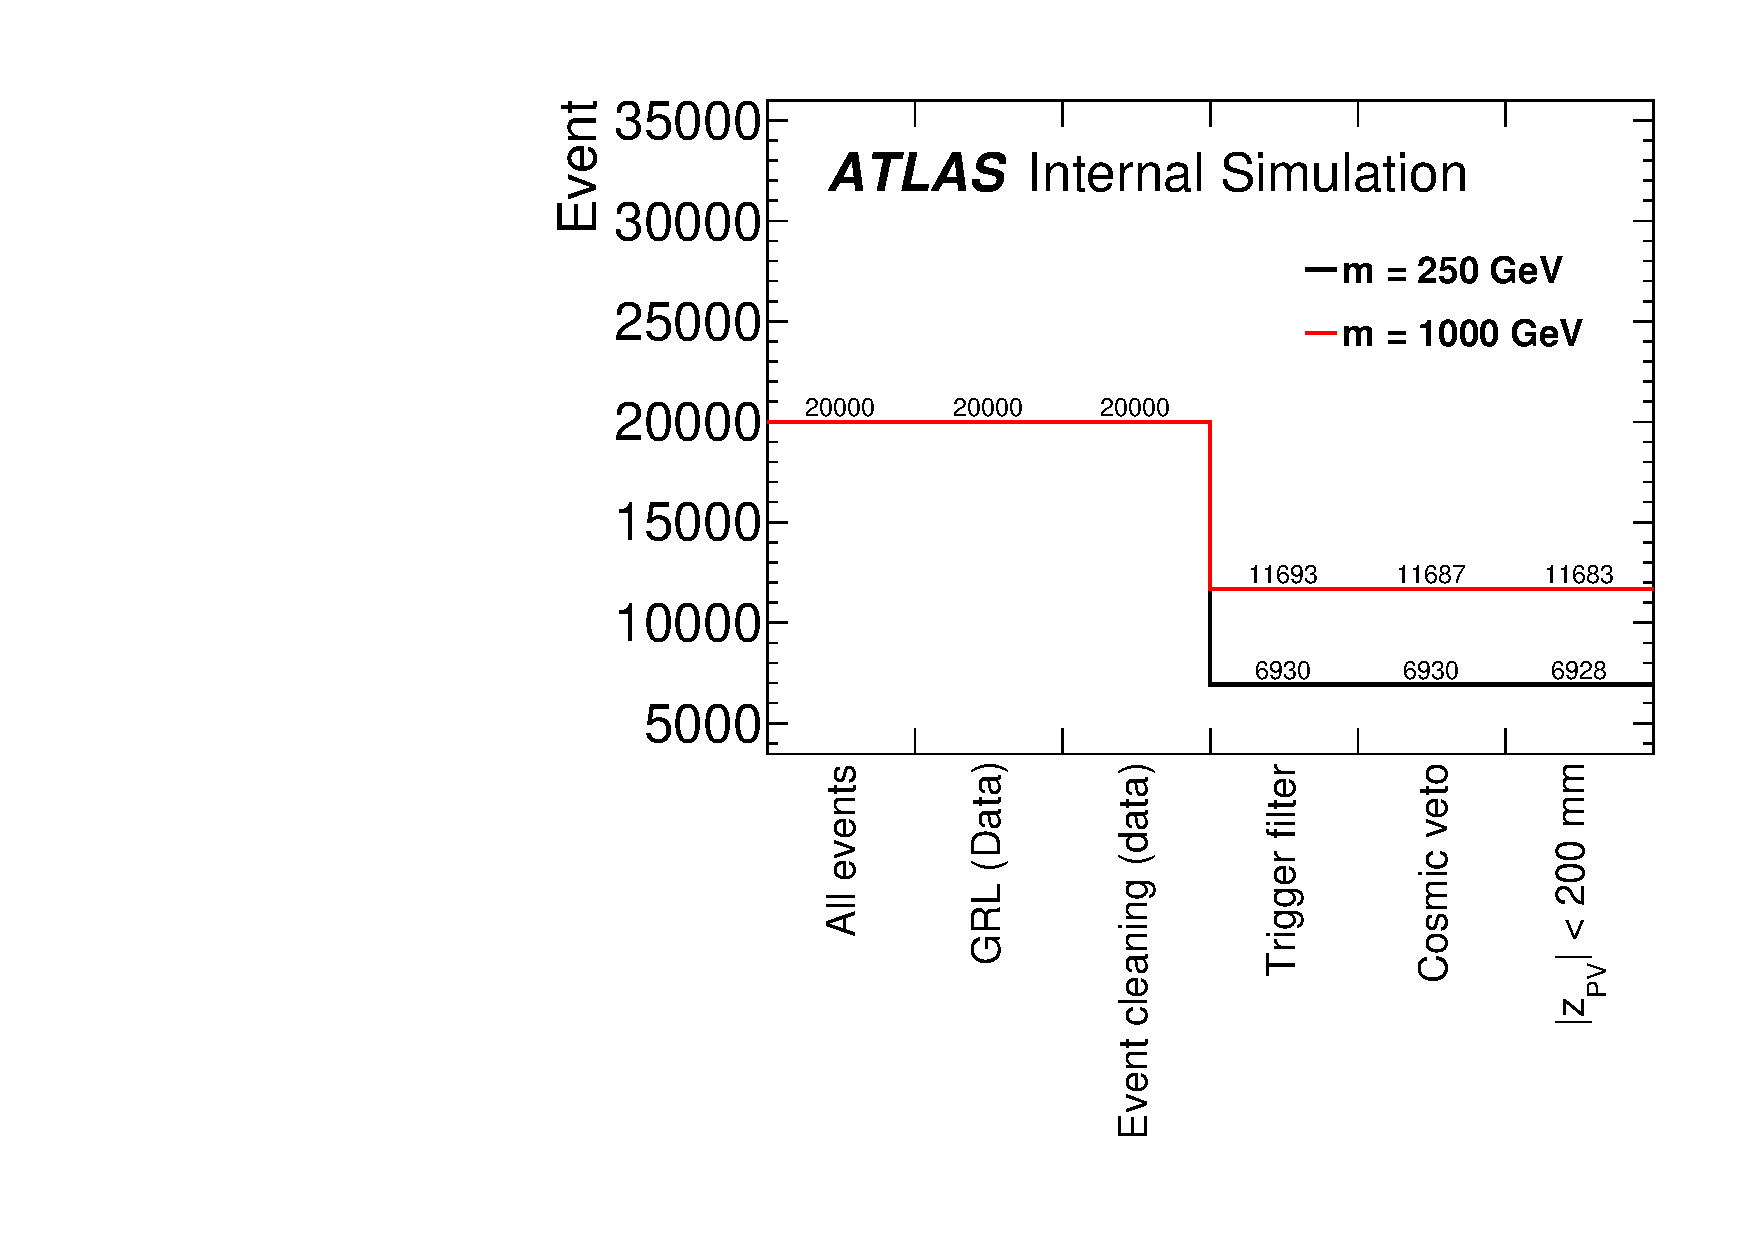
\includegraphics[width=0.5\textwidth]{figures/m_event_cutflow_MC_mumu.pdf}} 
    \subfloat[] {\label{subfig:vertex_cutflow_MC}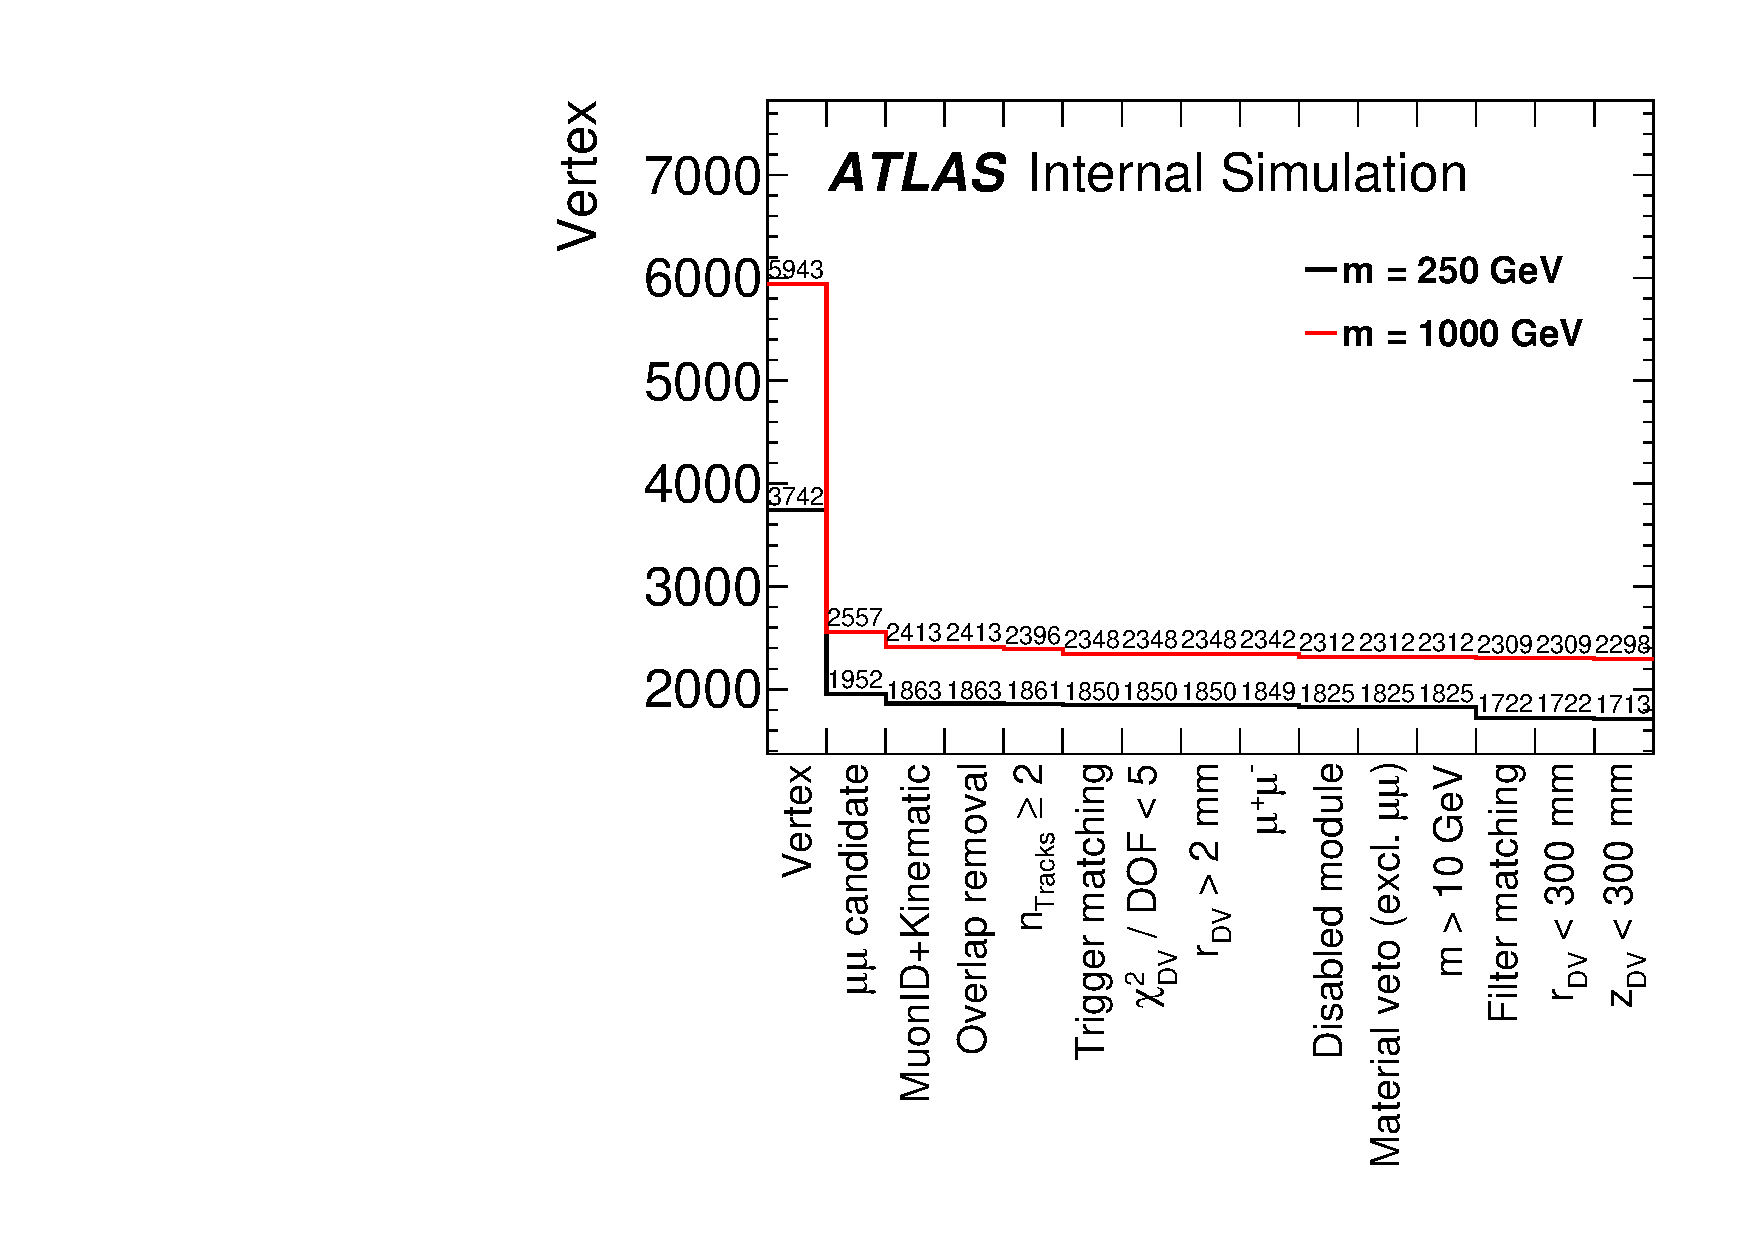
\includegraphics[width=0.5\textwidth]{figures/m_dv_cutflow_MC_mumu.pdf}} 
    \caption{(a) Event cut flow, and (b) vertex cut flow using the signal MC samples of $Z'\rightarrow \mumu$ generated with $m =$ 500, 1000 GeV for $c\tau= $ 100 mm.}
    \label{fig:signal_cutflow_MC_mumu}
\end{figure}

In the event cut flow, \texttt{GoodRunsList} filter and Event cleaning are shown as place holders as they are only applied to data sample. About 34-60$\%$ of signal events passed the event cut flow, but the vertex cut flow shows that only about 18-25$\%$ of signal events have a displaced vertex candidate, indicating that there is a significant loss of signal efficiency in the vertex reconstruction process. The following selection criteria, $\chi^{2} /$ DOF $<$ 5 and the displacement cut ($r_{DV} > $ 2 mm), are applied, but the effect is very small as expected because the same requirements are applied in the secondary vertex reconstruction algorithm. Material veto is applied to all vertex types except \mumu vertex. The minimum dilepton mass requirement has minimum impact on the signal efficiency.

Events and vertex cut flow of other signal samples are available in Table~\ref{table:cutflow_all}.


\begin{sidewaystable}[!htb]
  \centering
  \subfloat[$Z'\rightarrow \mumu$]{
  \resizebox{\textwidth}{!}{
  \begin{tabular}{ c c c c c c c c c c c c c c c c c c c c c}
    \hline
    \hline
    $m_{Z'}$ (GeV) & $c\tau$ (mm)   & \rot{All events} 
                                    & \rot{Trigger filter} 
                                    & \rot{Cosmic veto} 
                                    & \rot{$Z_{PV}<200$ mm} 
                                    & \rot{Vertex} 
                                    & \rot{$N_{\mu} \geq 2$ }
                                    & \rot{Muon selection} 
                                    & \rot{Overlap removal}
                                    & \rot{$N_{\mu}=2$}
                                    & \rot{Trigger matching}
                                    & \rot{$\chi^{2} /$ DOF $< 5$}
                                    & \rot{$r_{DV} >$ 2 mm}
                                    & \rot{\mumu}
                                    & \rot{Disabled module}
                                    & \rot{$m > 10$ GeV}
                                    & \rot{Filter matching}
                                    & \rot{$r_{DV} < 300$ mm}
                                    & \rot{$z_{DV} < 300$ mm} \\
    \hline
    100&	250&	20000&	818&	818&	818&	533&	269&	260&	260&	260&	259&	259&	259&	259&	252&	252&	82&	82&	81 \\
    100&	500&	20000&	761&	761&	761&	416&	165&	154&	154&	154&	154&	154&	154&	154&	148&	148&	50&	50&	49 \\
    100&	100&	20000&	940&	940&	940&	644&	366&	342&	342&	339&	339&	339&	339&	339&	330&	330&	108&	108&	106 \\
    250&	250&	20000&	6180&	6179&	6176&	3467&	1809&	1708&	1708&	1703&	1700&	1700&	1700&	1699&	1677&	1677&	1605&	1605&	1582 \\
    250&	500&	20000&	4922&	4921&	4921&	2680&	1354&	1284&	1284&	1278&	1276&	1276&	1276&	1276&	1261&	1261&	1205&	1205&	1176 \\
    250&	100&	20000&	6930&	6930&	6928&	3742&	1952&	1863&	1863&	1861&	1850&	1850&	1850&	1849&	1825&	1825&	1722&	1722&	1713 \\
    500&	500&	20000&	6724&	6720&	6717&	3605&	1777&	1666&	1666&	1658&	1646&	1646&	1646&	1646&	1617&	1617&	1611&	1611&	1572 \\
    500&	250&	20000&	8273&	8272&	8269&	4481&	2191&	2080&	2080&	2068&	2056&	2056&	2056&	2054&	2024&	2024&	2023&	2023&	2007 \\
    500&	100&	19000&	9146&	9145&	9144&	4680&	2205&	2091&	2091&	2085&	2068&	2068&	2068&	2068&	2047&	2047&	2042&	2042&	2034 \\
    750&	100&	20000&	11032&	11028&	11027&	5605&	2473&	2330&	2330&	2313&	2282&	2282&	2282&	2281&	2267&	2267&	2254&	2254&	2250 \\
    750&	500&	20000&	8059&	8055&	8054&	4262&	2017&	1878&	1878&	1868&	1851&	1851&	1851&	1849&	1824&	1824&	1820&	1819&	1784 \\
    750&	250&	20000&	9622&	9616&	9613&	5301&	2626&	2457&	2457&	2441&	2421&	2421&	2421&	2419&	2391&	2391&	2386&	2385&	2364 \\
    1000&	250&	20000&	10517&	10515&	10514&	5804&	2725&	2578&	2578&	2564&	2518&	2518&	2517&	2512&	2479&	2479&	2476&	2476&	2457 \\
    1000&	100&	20000&	11693&	11687&	11683&	5943&	2557&	2413&	2413&	2396&	2348&	2348&	2348&	2342&	2312&	2312&	2309&	2309&	2298 \\
    1000&	500&	20000&	8905&	8902&	8901&	4878&	2295&	2170&	2170&	2155&	2129&	2129&	2129&	2117&	2092&	2092&	2089&	2089&	2058 \\
    \hline
    \hline
  \end{tabular}
  }}

  \caption{Event and vertex cut flow of signal samples}
  \label{table:cutflow_all}
\end{sidewaystable}

\begin{sidewaystable}[!htb]\ContinuedFloat
  \centering
  \subfloat[$Z'\rightarrow \ee$]{
  \resizebox{\textwidth}{!}{
  \begin{tabular}{ c c c c c c c c c c c c c c c c c c c c c c}
    \hline
    \hline
    $m_{Z'}$ (GeV) & $c\tau$ (mm)   & \rot{All events} 
                                    & \rot{Trigger filter} 
                                    & \rot{Cosmic veto} 
                                    & \rot{$Z_{PV}<200$ mm} 
                                    & \rot{Vertex} 
                                    & \rot{$N_{e} \geq 2$ }
                                    & \rot{Electron selection} 
                                    & \rot{Bad cluster} 
                                    & \rot{Overlap removal}
                                    & \rot{$N_{e} = 2$}
                                    & \rot{Trigger matching}
                                    & \rot{$\chi^{2} /$ DOF $< 5$}
                                    & \rot{$r_{DV} > 2$ mm}
                                    & \rot{\ee}
                                    & \rot{Disabled module}
                                    & \rot{Material veto}
                                    & \rot{$m > 10$ GeV}
                                    & \rot{Filter matching}
                                    & \rot{$r_{DV} < 300$ mm}
                                    & \rot{$z_{DV} < 300$ mm} \\
    \hline
    100&	250&	20000&	323&	323&	323&	145&	61&	59&	58&	56&	56&	56&	56&	56&	56&	55&	36&	36&	15&	15&	15 \\
    100&	500&	20000&	241&	241&	241&	111&	31&	30&	29&	29&	29&	27&	27&	27&	27&	26&	19&	19&	10&	10&	9 \\
    100&	100&	20000&	315&	315&	315&	166&	71&	69&	69&	67&	67&	66&	66&	66&	66&	65&	52&	52&	16&	16&	15 \\
    250&	250&	20000&	9276&	9274&	9272&	4083&	1576&	1519&	1501&	1477&	1458&	1453&	1453&	1453&	1448&	1417&	1206&	1206&	1174&	1174&	1163 \\
    250&	500&	20000&	7755&	7750&	7749&	3203&	1105&	1063&	1057&	1038&	1017&	1011&	1011&	1011&	1007&	987&	803&	803&	769&	769&	758 \\
    250&	100&	20000&	10147&	10145&	10144&	4472&	1696&	1658&	1639&	1618&	1601&	1585&	1585&	1585&	1577&	1563&	1378&	1378&	1345&	1345&	1339 \\
    500&	500&	19000&	12279&	12278&	12276&	5029&	1566&	1505&	1502&	1493&	1471&	1466&	1466&	1466&	1455&	1432&	1194&	1194&	1185&	1185&	1162 \\
    500&	250&	20000&	14855&	14853&	14849&	6245&	1986&	1907&	1892&	1880&	1858&	1858&	1858&	1857&	1844&	1824&	1580&	1580&	1569&	1569&	1559 \\
    500&	100&	20000&	16012&	16008&	16006&	6621&	2017&	1940&	1925&	1900&	1878&	1877&	1877&	1877&	1857&	1843&	1668&	1668&	1656&	1656&	1652 \\
    750&	100&	20000&	18014&	18011&	18006&	7422&	2266&	2196&	2182&	2173&	2138&	2138&	2138&	2138&	2092&	2085&	1919&	1919&	1914&	1914&	1913 \\
    750&	500&	20000&	15290&	15286&	15283&	6206&	1853&	1791&	1778&	1768&	1731&	1731&	1731&	1731&	1711&	1690&	1423&	1423&	1419&	1419&	1399 \\
    750&	250&	20000&	16920&	16914&	16912&	7165&	2260&	2186&	2177&	2168&	2129&	2129&	2129&	2129&	2099&	2081&	1832&	1832&	1824&	1824&	1808 \\
    1000&	250&	20000&	17890&	17883&	17877&	7674&	2487&	2412&	2401&	2395&	2349&	2349&	2349&	2349&	2320&	2298&	2070&	2070&	2067&	2067&	2050 \\
    1000&	100&	20000&	18723&	18719&	18714&	7749&	2347&	2271&	2247&	2235&	2195&	2195&	2195&	2195&	2162&	2151&	2004&	2004&	1996&	1996&	1992 \\
    1000&	500&	19000&	15666&	15660&	15658&	6507&	1956&	1881&	1870&	1866&	1842&	1842&	1842&	1842&	1812&	1797&	1562&	1562&	1559&	1559&	1548 \\
    \hline
    \hline
  \end{tabular}
  }}
  \caption{Event and vertex cut flow of signal samples}
  \label{table:cutflow_all}
\end{sidewaystable}

\begin{sidewaystable}[!htb]\ContinuedFloat
  \centering
  \subfloat[$Z'\rightarrow \emu$]{
  \resizebox{\textwidth}{!}{
  \begin{tabular}{ c c c c c c c c c c c c c c c c c c c c c c}
    \hline
    \hline
    $m_{Z'}$ (GeV) & $c\tau$ (mm)   & \rot{All events} 
                                    & \rot{Trigger filter} 
                                    & \rot{Cosmic veto} 
                                    & \rot{$Z_{PV} < 200$ mm} 
                                    & \rot{Vertex} 
                                    & \rot{$N_{\ell} \geq 2$ }
                                    & \rot{Electron selection} 
                                    & \rot{Bad cluster} 
                                    & \rot{Overlap removal}
                                    & \rot{$N_{\ell} = 2$}
                                    & \rot{Trigger matching}
                                    & \rot{$\chi^{2} /$ DOF $< 5$}
                                    & \rot{$r_{DV} > 2$ mm}
                                    & \rot{\emu}
                                    & \rot{Disabled module}
                                    & \rot{Material veto}
                                    & \rot{$m > 10$ GeV}
                                    & \rot{Filter matching}
                                    & \rot{$r_{DV} < 300$ mm}
                                    & \rot{$z_{DV} < 300$ mm} \\
    \hline
    100&	250&	20000&	483&	483&	483&	255&	94&	91&	91&	89&	88&	88&	88&	88&	88&	87&	61&	61&	21&	21&	19 \\
    100&	500&	19000&	379&	379&	379&	178&	56&	53&	53&	53&	53&	53&	53&	53&	53&	50&	34&	34&	15&	15&	14 \\
    100&	100&	19000&	484&	484&	484&	295&	150&	145&	145&	137&	136&	134&	134&	134&	134&	127&	88&	88&	26&	26&	26 \\
    250&	250&	20000&	4273&	4272&	4265&	2251&	921&	901&	899&	874&	867&	848&	848&	848&	844&	829&	682&	682&	650&	650&	638 \\
    250&	500&	20000&	3486&	3484&	3481&	1667&	709&	695&	693&	678&	672&	663&	663&	663&	662&	653&	532&	532&	511&	511&	502 \\
    250&	100&	20000&	4771&	4769&	4768&	2326&	960&	938&	934&	899&	891&	868&	868&	868&	862&	851&	729&	729&	698&	698&	696 \\
    500&	500&	20000&	10885&	10883&	10883&	4797&	1732&	1697&	1689&	1623&	1604&	1595&	1594&	1594&	1581&	1552&	1327&	1327&	1264&	1264&	1239 \\
    500&	250&	20000&	12680&	12680&	12679&	5736&	2199&	2169&	2160&	2059&	2037&	2020&	2020&	2019&	2016&	1990&	1748&	1748&	1688&	1688&	1671 \\
    500&	100&	19000&	13351&	13349&	13346&	6049&	2168&	2135&	2131&	2040&	2019&	2005&	2005&	2005&	1999&	1981&	1793&	1793&	1736&	1736&	1728 \\
    750&	100&	19000&	16046&	16036&	16032&	7041&	2624&	2590&	2582&	2480&	2448&	2437&	2437&	2436&	2408&	2400&	2232&	2232&	2207&	2207&	2203 \\
    750&	500&	20000&	13598&	13590&	13585&	6033&	2170&	2132&	2125&	2025&	2003&	1995&	1995&	1995&	1983&	1965&	1686&	1686&	1644&	1644&	1604 \\
    750&	250&	20000&	15546&	15545&	15541&	7171&	2706&	2659&	2655&	2533&	2502&	2494&	2493&	2492&	2475&	2448&	2172&	2172&	2142&	2142&	2115 \\
    1000&	250&	20000&	16751&	16743&	16739&	7835&	3088&	3036&	3028&	2899&	2856&	2854&	2854&	2854&	2832&	2809&	2512&	2512&	2495&	2495&	2475 \\
    1000&	100&	18000&	15970&	15963&	15959&	7189&	2581&	2543&	2535&	2415&	2385&	2371&	2371&	2370&	2345&	2323&	2163&	2163&	2148&	2148&	2146 \\
    1000&	500&	19000&	14165&	14160&	14154&	6366&	2345&	2290&	2284&	2198&	2162&	2153&	2153&	2152&	2134&	2112&	1826&	1825&	1808&	1808&	1773 \\
    \hline
    \hline
  \end{tabular}
  }}
  \caption{Event and vertex cut flow of signal samples}
  \label{table:cutflow_all}
\end{sidewaystable}




\subsection{Signal efficiency and distribution}
\label{sec:efficiency}

The signal efficiency is studied by examining the efficiency distributions in the transverse ($r$), longitudinal ($z$) vertex position, and the angular distributions of the signal vertices. The representative efficiency distributions are shown in Figure~\ref{fig:signal_vertex_dist} using the signal MC samples generated with $m =$ 500, 1000 GeV for $c\tau=$ 100 mm.

\begin{figure}[!htb]
    \centering
    \subfloat[]{\label{subfig:vertex_dist_r  }\includegraphics[width=0.49\textwidth]{figures/m_eff_dv_r.pdf}}
    \subfloat[]{\label{subfig:vertex_dist_z  }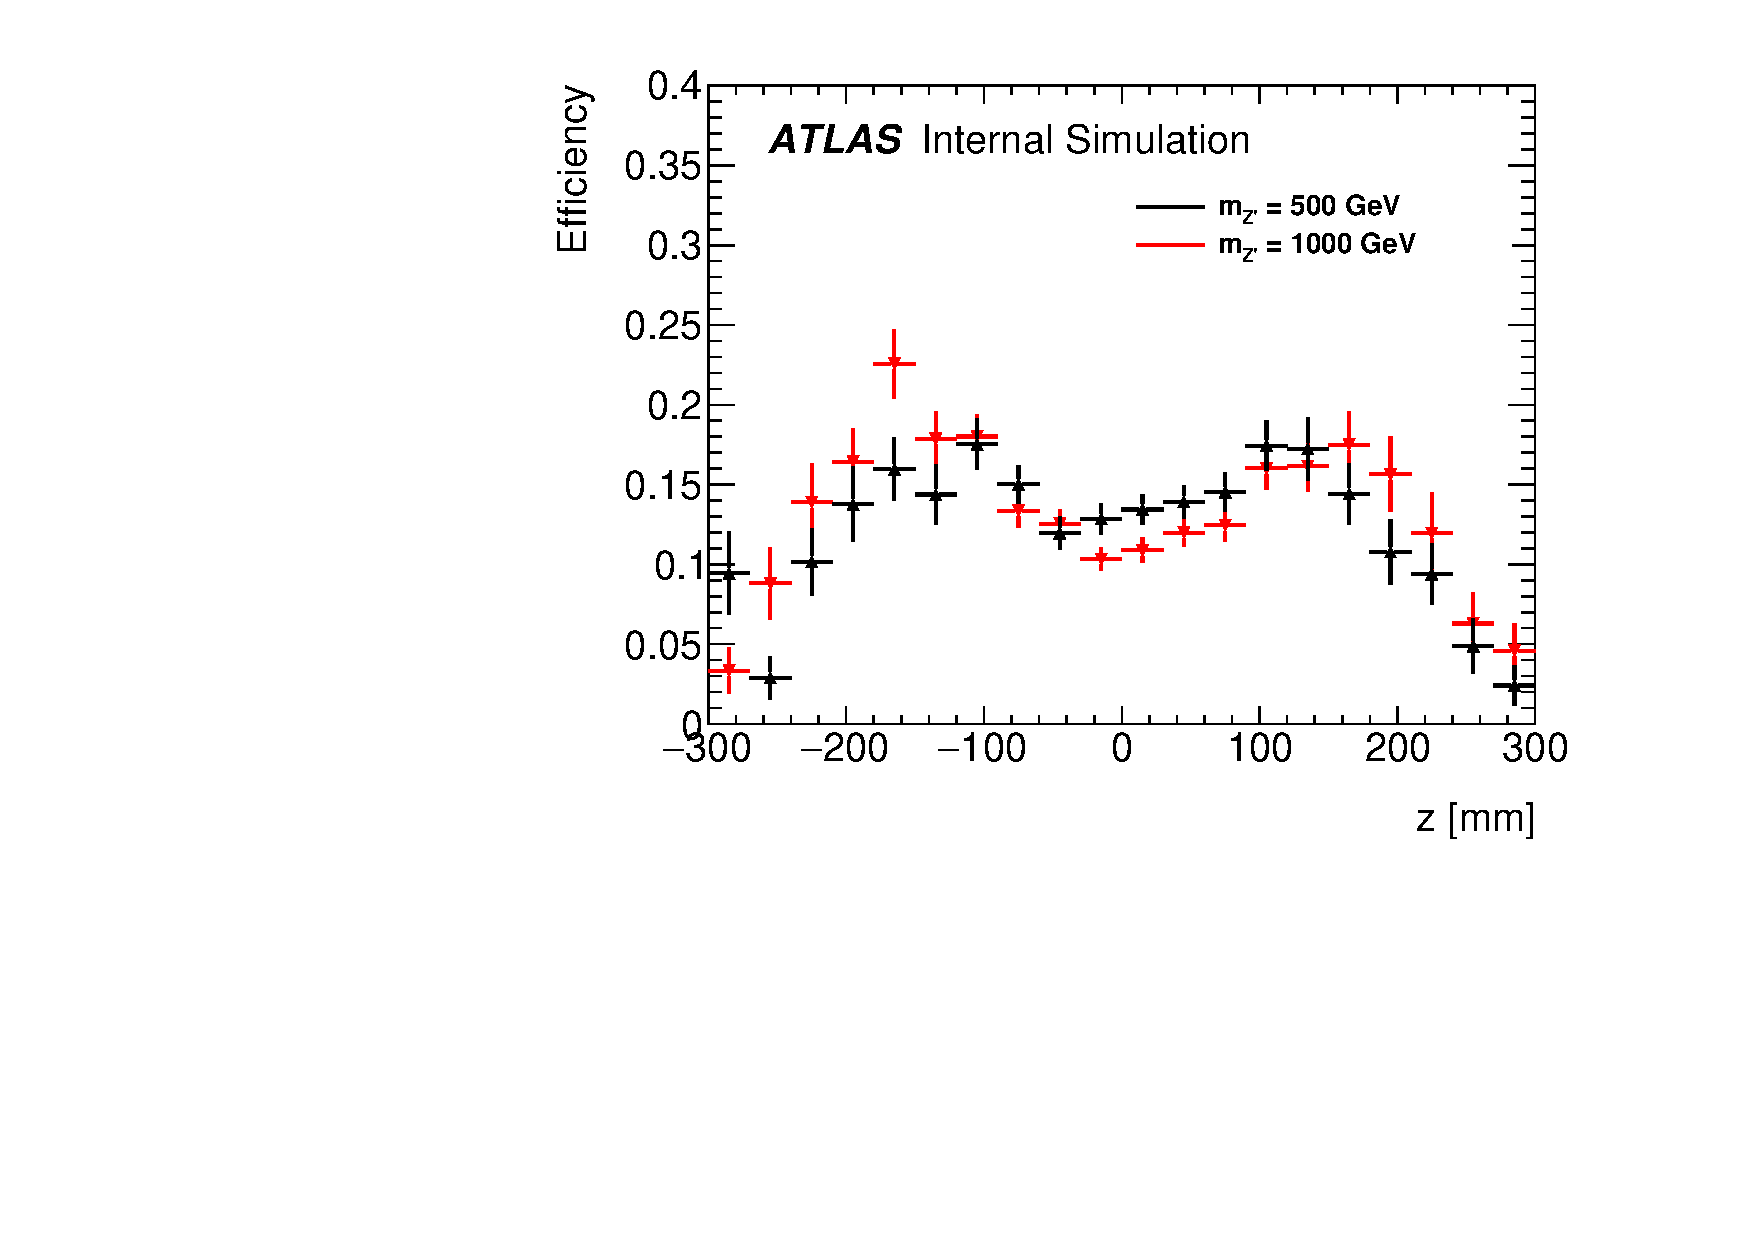
\includegraphics[width=0.49\textwidth]{figures/m_eff_dv_z.pdf}} \\
    \subfloat[]{\label{subfig:vertex_dist_eta}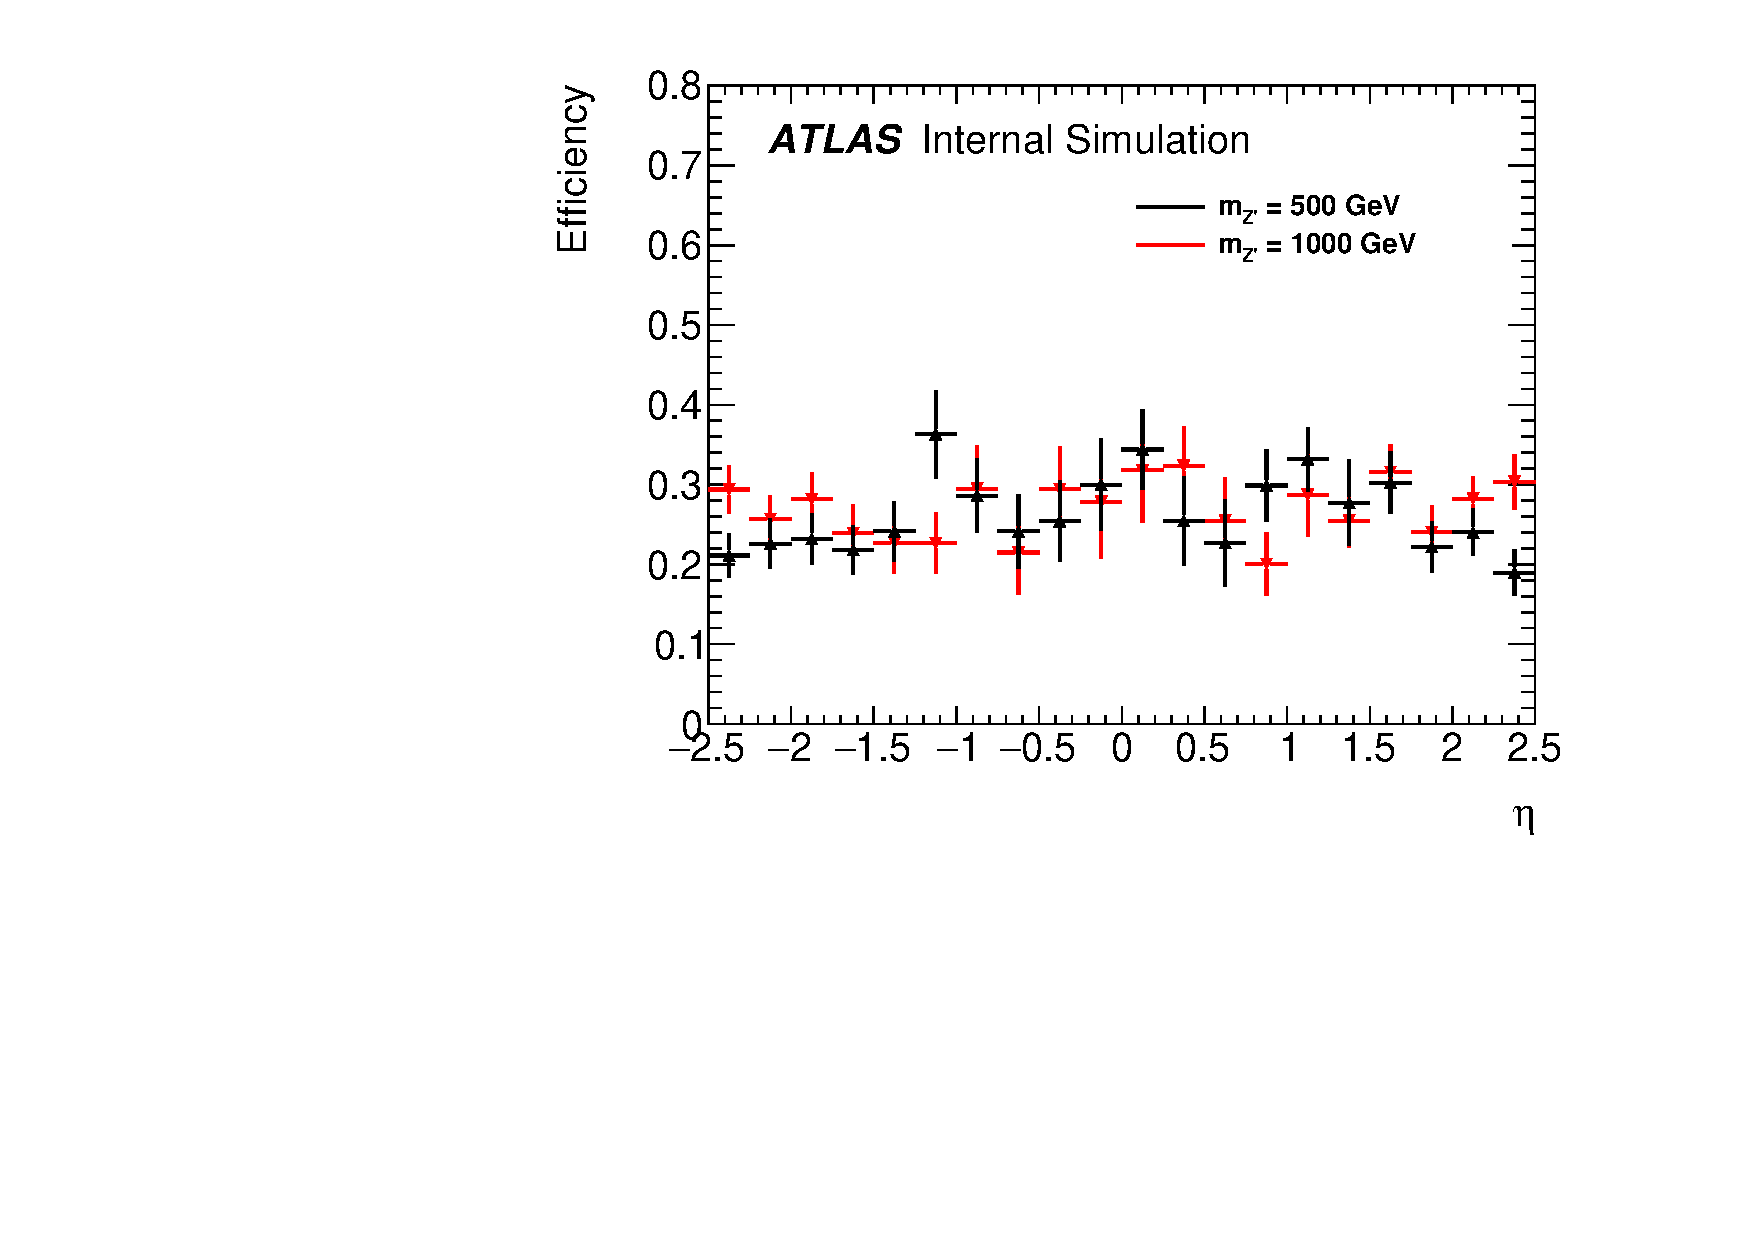
\includegraphics[width=0.49\textwidth]{figures/m_eff_dv_eta.pdf}}
    \subfloat[]{\label{subfig:vertex_dist_phi}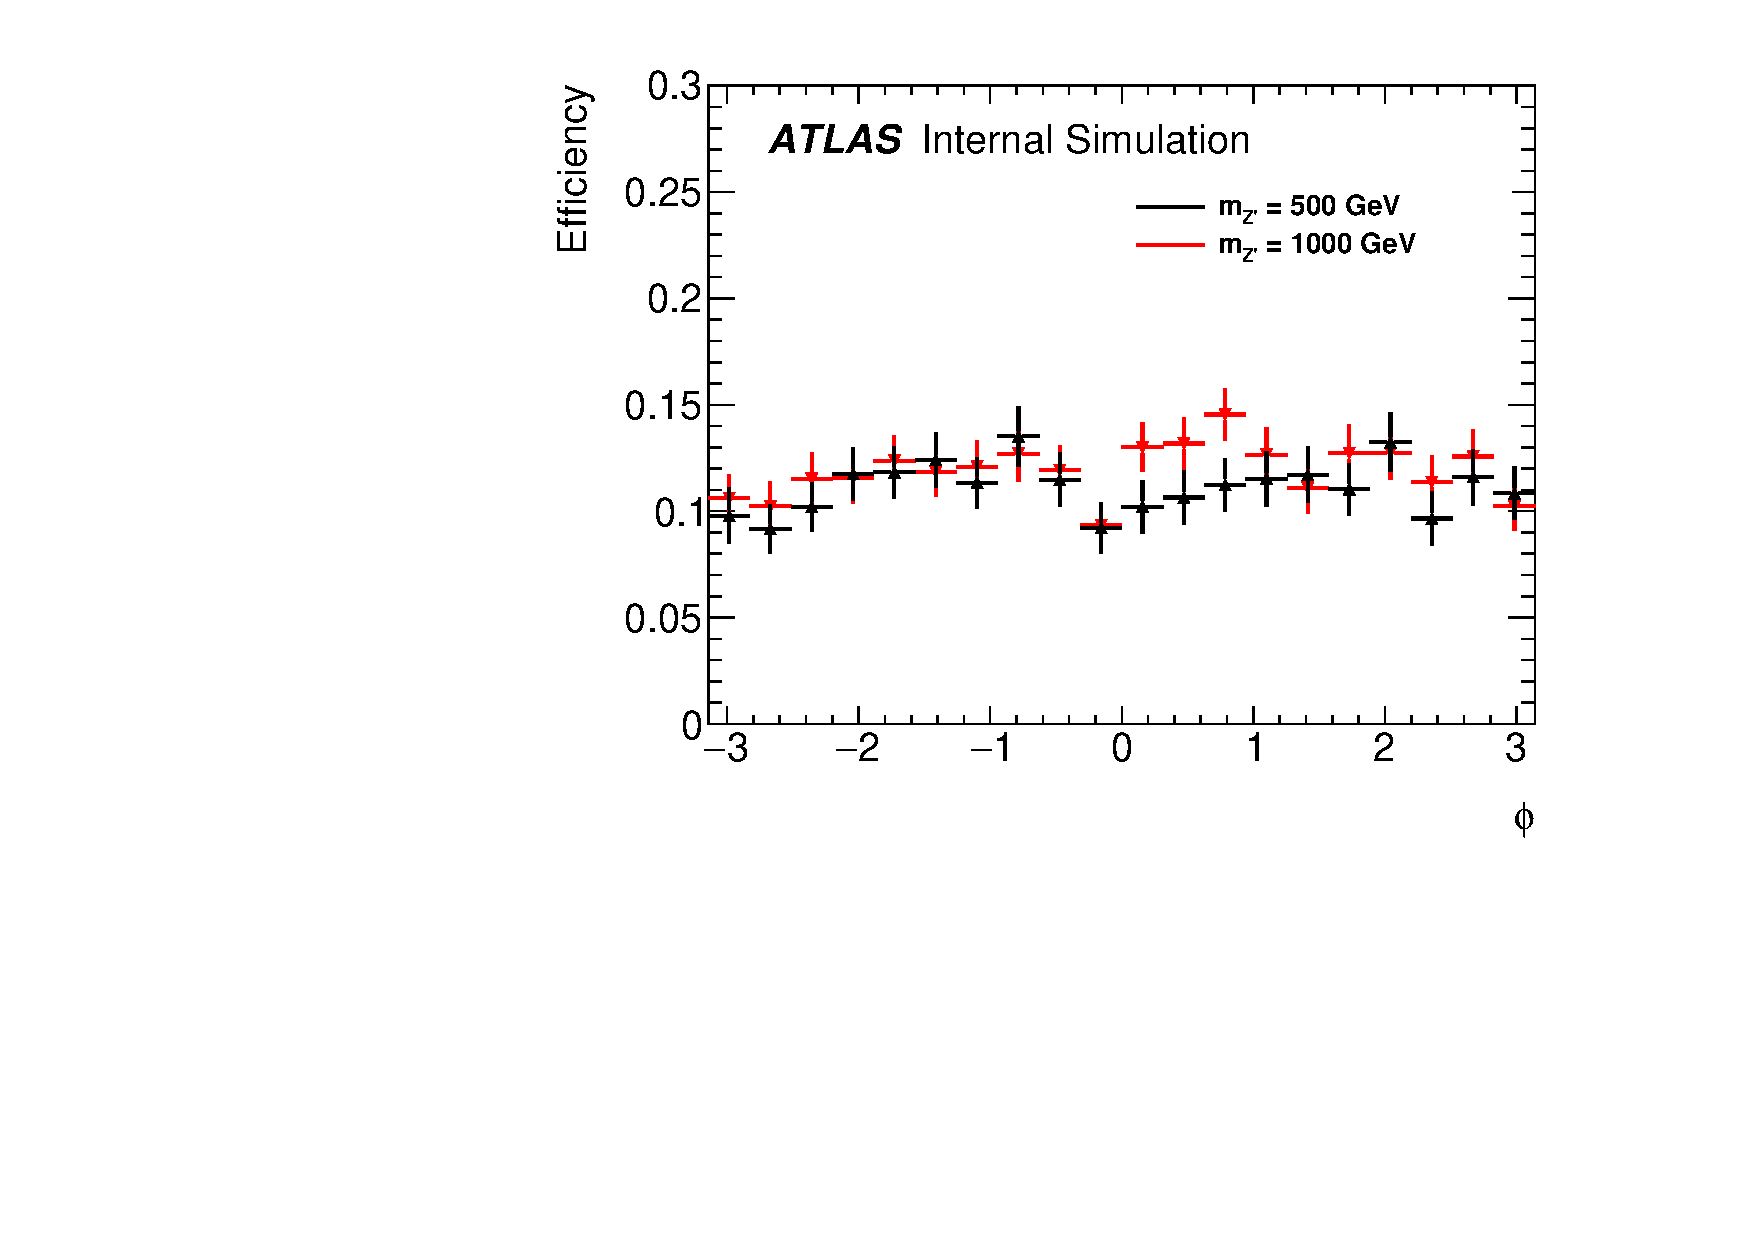
\includegraphics[width=0.49\textwidth]{figures/m_eff_dv_phi.pdf}}\\
    \subfloat[]{\label{subfig:vertex_dist_r  }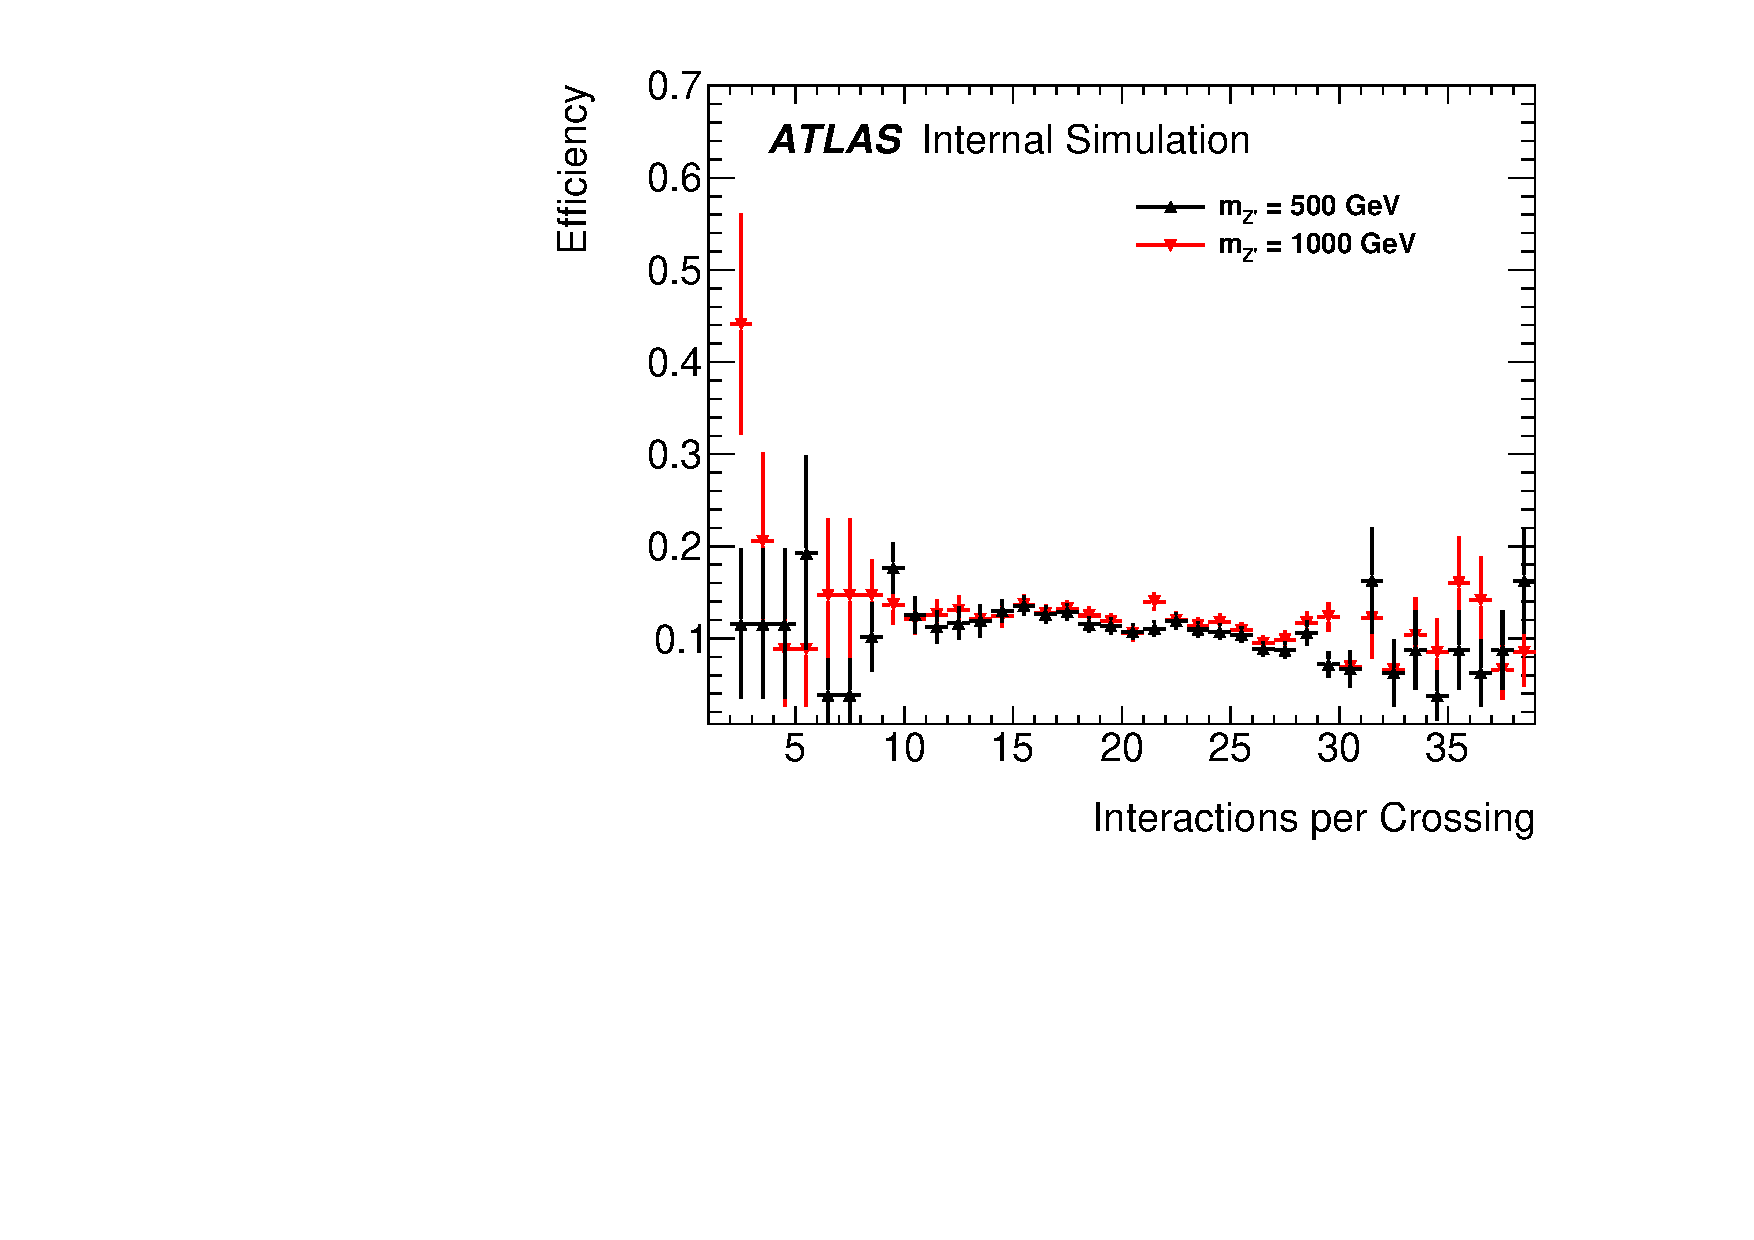
\includegraphics[width=0.49\textwidth]{figures/dv_eff_mu_zp.pdf}}
    \caption{Signal efficiency distributions in (a) $r$, (b) $z$, (c) $\eta$, (d) $\phi$, and (e) pile-up of the signal MC samples of $Z'\rightarrow \mumu$ with $m=$ 500, 1000 GeV for $c\tau=$ 100 mm.}
    \label{fig:signal_vertex_dist}
\end{figure}


The signal efficiency shows a dependence on vertex position which decreases at large $r$ and $z$ due to the minimum silicon hits requirement on tracks. The first (central) bins in $r$ ($z$) distributions have lower efficiency due to the minimum displacement requirement ($r_{DV} > $ 2 mm) on secondary vertices. The $\eta$ distribution has higher efficiency than overall efficiency in the tracking region ($|\eta| < 2.5$), and the $\phi$ distribution is uniform as expected. Pile-up distribution of the signal efficiency shows that the efficiency is reduced for high pile-up as expected.

The overall signal efficiency for the signal samples are shown in Table~\ref{table:signal_eff}. The signal efficiency ranges from 14.9-33.3\% for mass above 500 GeV, but the efficiency is reduced for lower $Z'$ mass due to minimum $p_{T}$ thresholds on the leptons, especially for the samples with $m_{Z'}=100~\si{\GeV}$. The samples with shorter lifetime tend to have higher signal efficiency as expected. 

\begin{table}[!htb]
  \centering
  \begin{tabular}{ c c @{\hspace{1cm}} c @{\hspace{1cm}} c @{\hspace{1cm}} c }
    \hline
    \hline
    $m_{Z'}$ (GeV) & $c\tau$ (mm)   &$\mu\mu$  & $ee$  & $e\mu$ \\
    \hline
    100			   &  100	        &0.004	&0.001	&0.001   \\
    100			   &  250	        &0.002	&0.000	&0.001   \\
    100			   &  500	        &0.005	&0.001	&0.001   \\
    250			   &  100	        &0.079	&0.058	&0.032   \\
    250			   &  250	        &0.059	&0.038	&0.025   \\
    250			   &  500	        &0.086	&0.067	&0.035   \\
    500			   &  100	        &0.079	&0.061	&0.062   \\
    500			   &  250	        &0.100	&0.078	&0.084   \\
    500			   &  500	        &0.107	&0.083	&0.091   \\
    750			   &  100	        &0.113	&0.096	&0.116   \\
    750			   &  250	        &0.089	&0.070	&0.080   \\
    750			   &  500	        &0.118	&0.090	&0.106   \\
    1000	       &  100	        &0.123	&0.103	&0.124   \\
    1000	       &  250	        &0.115	&0.100	&0.119   \\
    1000	       &  500	        &0.103	&0.081	&0.093   \\
    \hline
    \hline
  \end{tabular}
  \caption{Overall signal efficiency of the signal samples.}
  \label{table:signal_eff}
\end{table}




\subsection{Efficiency map}
\label{sec:efficiency_map}
Signal efficiency for each mass and lifetime of long-lived $Z'$ sample is presented as a function of $p_{T}$ and $\eta$ of $Z'$. Because any neutral, LLP decaying to a dilepton pair can be mostly described by mass, lifetime, $p_{T}$, and $\eta$ of the LLP, these efficiency maps can be used for other BSM searches such as searching for long-lived neutralino in the context of SUSY R-parity violating theory.

Representative efficiency maps are shown in Figure~\ref{fig:signal_eff_map} using the signal MC samples of $Z' \rightarrow \mumu$ with $m=$ 500, 1000 GeV and $c\tau=$ 100, 500 mm. Although the overall signal efficiency is $\sim$10\% for these samples, the efficiencies in the central region of the efficiency maps are much higher but much reduced in the forward region ($\eta > 2.5$) due to limited coverage. Efficiency maps of other signal samples are available in Appendix~\ref{app:signal_efficiency_map}.

\begin{figure}[!htb]
    \centering
    \subfloat[]{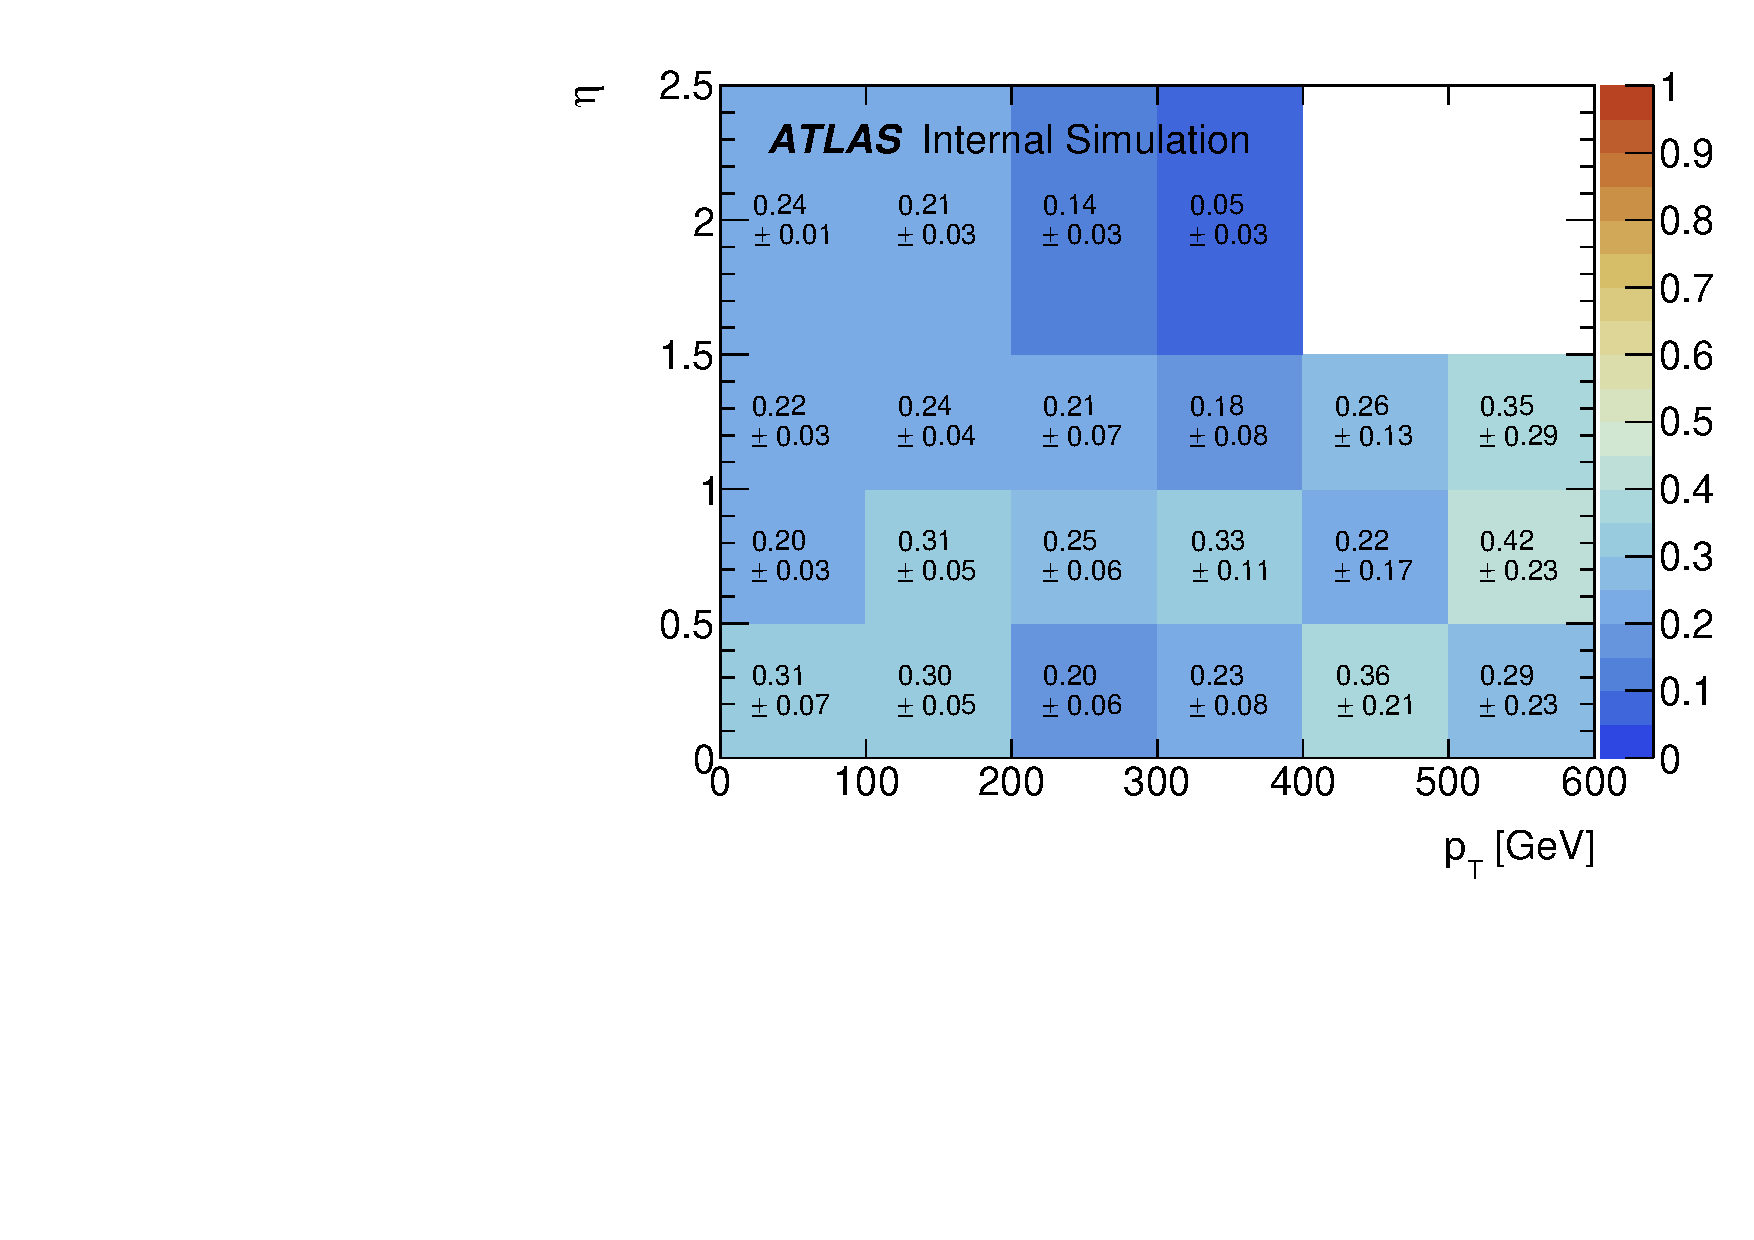
\includegraphics[width=0.50\textwidth]{figures/EfficiencyMap/eff_map_mumu_m500t100.pdf}}
    \subfloat[]{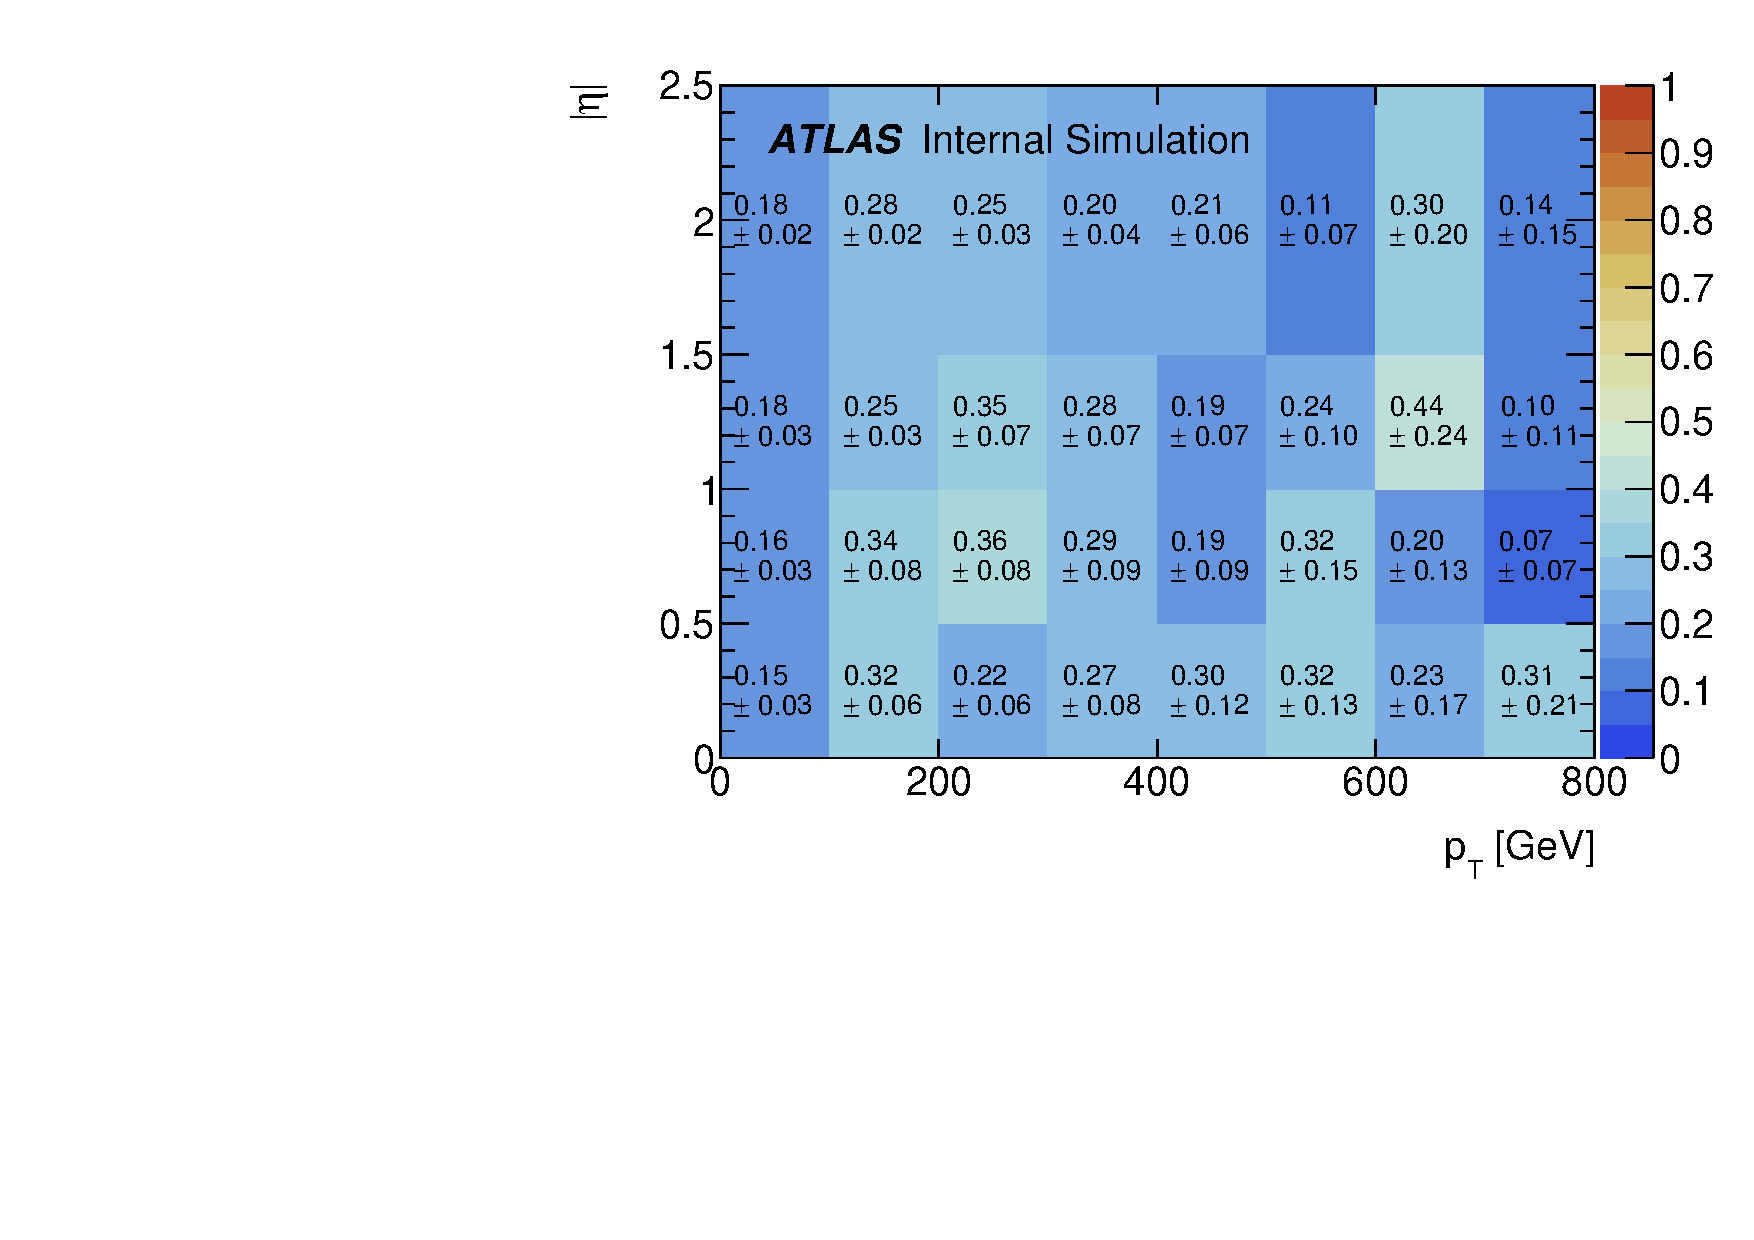
\includegraphics[width=0.50\textwidth]{figures/EfficiencyMap/eff_map_mumu_m1000t100.pdf}} \\
    \subfloat[]{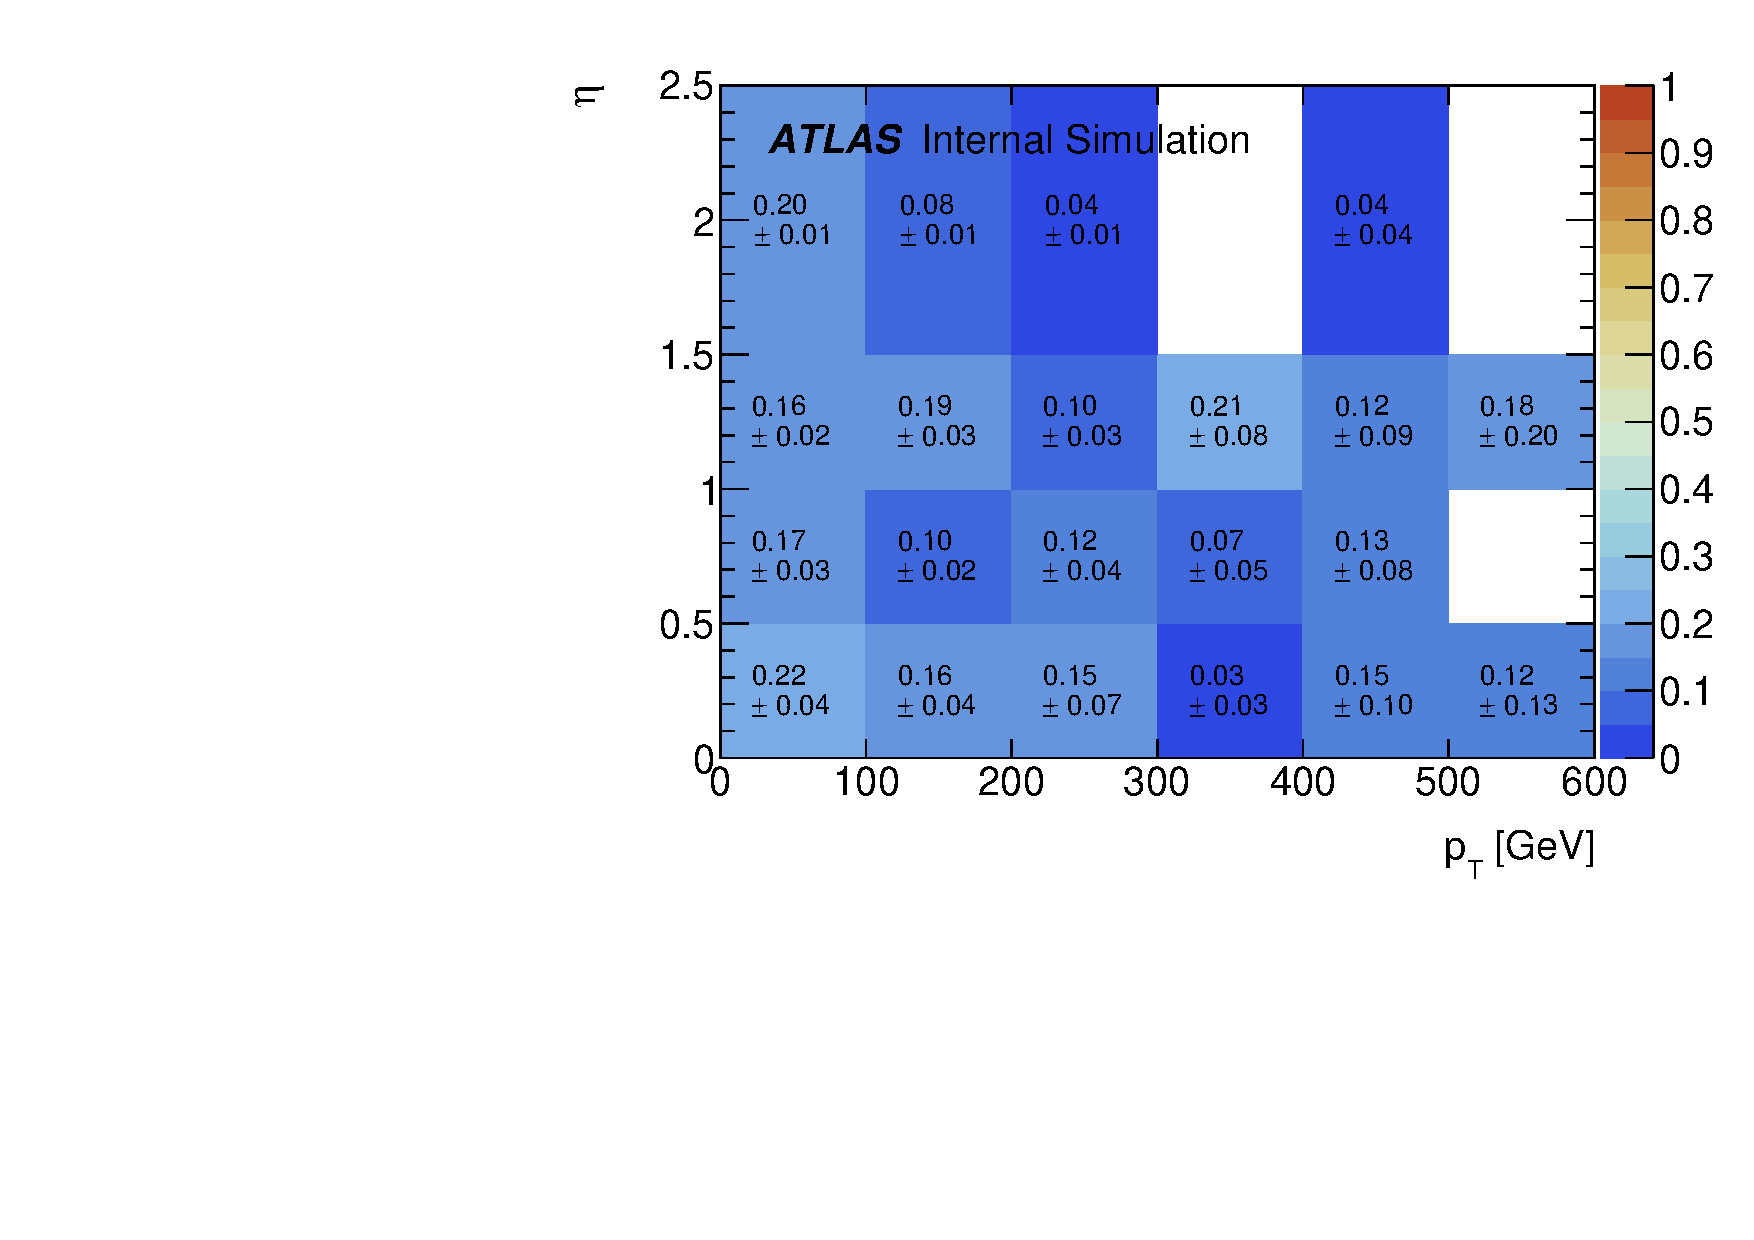
\includegraphics[width=0.50\textwidth]{figures/EfficiencyMap/eff_map_mumu_m500t500.pdf}}
    \subfloat[]{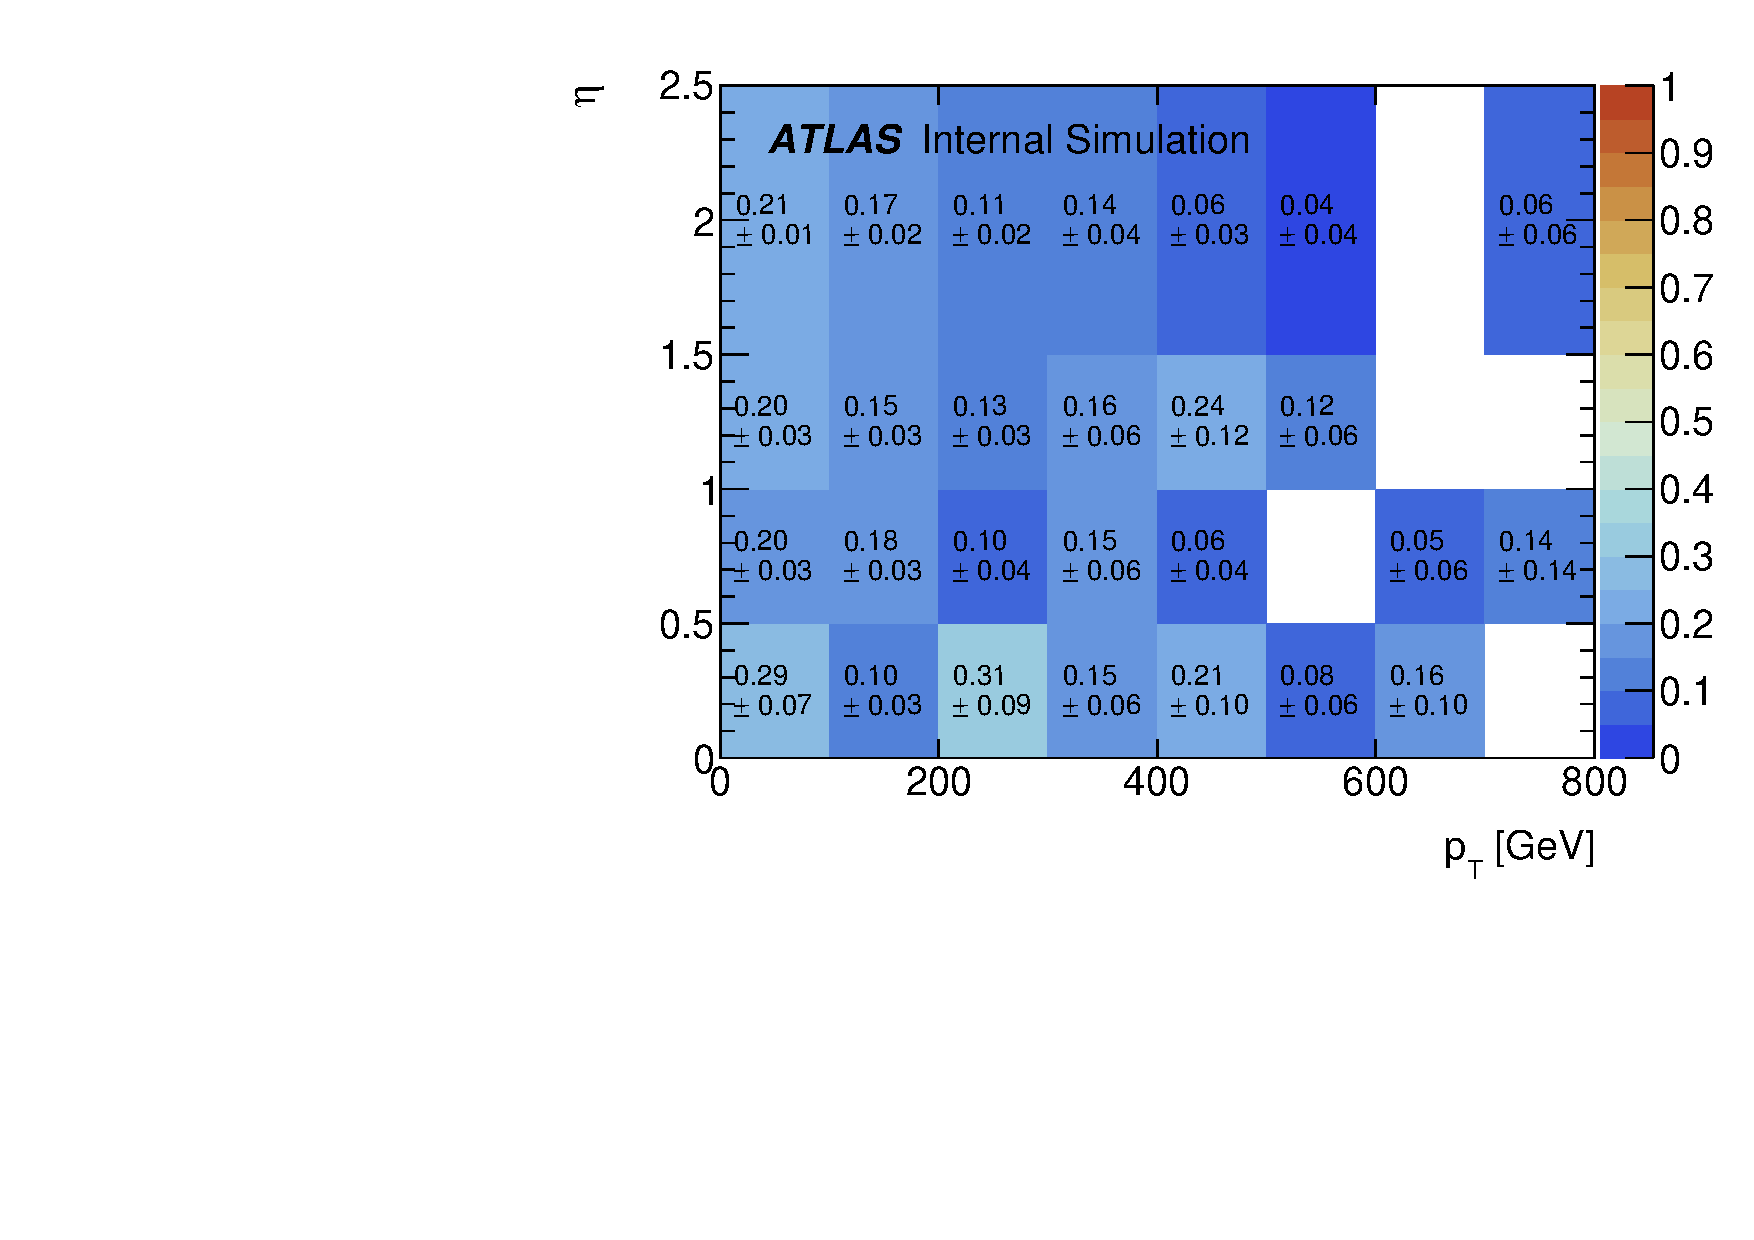
\includegraphics[width=0.50\textwidth]{figures/EfficiencyMap/eff_map_mumu_m1000t500.pdf}} \\
    \caption{Signal efficiency map of the signal MC sample with (a) $m=500$ and (b) $m=1000$ GeV for $c\tau=$ 100 mm. The corresponding efficiency map for $c\tau=$ 500 mm is shown in (c) and (d).}
    \label{fig:signal_eff_map}
\end{figure}





\chapter{Background Estimation}
\label{chap:bkg}

Due to the lifetime ($c\tau > 2$ mm) and mass ($m > 10$ GeV) requirements applied at vertex selection, no SM background is expected in the signal region in the search for a displaced dilepton resonance. Therefore, two non-collision backgrounds are considered in this search: cosmic background and \textit{random-crossing} background. The cosmic background is the dominant background in this analysis and is estimated in Section~\ref{sec:bkg:cosmic}. In Section~\ref{sec:bkg:random}, the background from the random-crossing of two uncorrelated tracks is estimated.


\section{Cosmic Background}
\label{sec:bkg:cosmic}

A cosmic muon passing through the ID during a collision event can be reconstructed as a back-to-back muon pair with opposite electric charges, forming a displaced \mumu vertex.

This cosmic background is suppressed by implementing the cosmic veto, $R_{\mathrm{CR}} < 0.01$ (Section~\ref{sec:event_selection}). The event cut flow in Figure~\ref{subfig:event_cutflow_MC} shows that the cosmic veto is very effective with negligible signal loss. To illustrate the effectiveness of the veto, a cosmic control region is defined as follows:

\begin{itemize}
  \item Events are required to fail the cosmic veto.
  \item Events are required to have at least two muons satisfying vertex track selection (Table~\ref{table:vertex_track_selection_simple}).
  \item All other event selections are kept the same as the signal region.
\end{itemize}

In this control region, pairs of two muons with highest $p_{T}$ are studied using the data sample. Figure~\ref{fig:cosmicData} shows the distribution of the pairs in $|\Delta\phi|$ and $\eta_{1}+\eta_{2}$. The distribution shows that a significant faction of muons pairs is from cosmic rays and is constrained to the small \Rcr region.

\begin{figure}[!htb]
    \begin{center}
    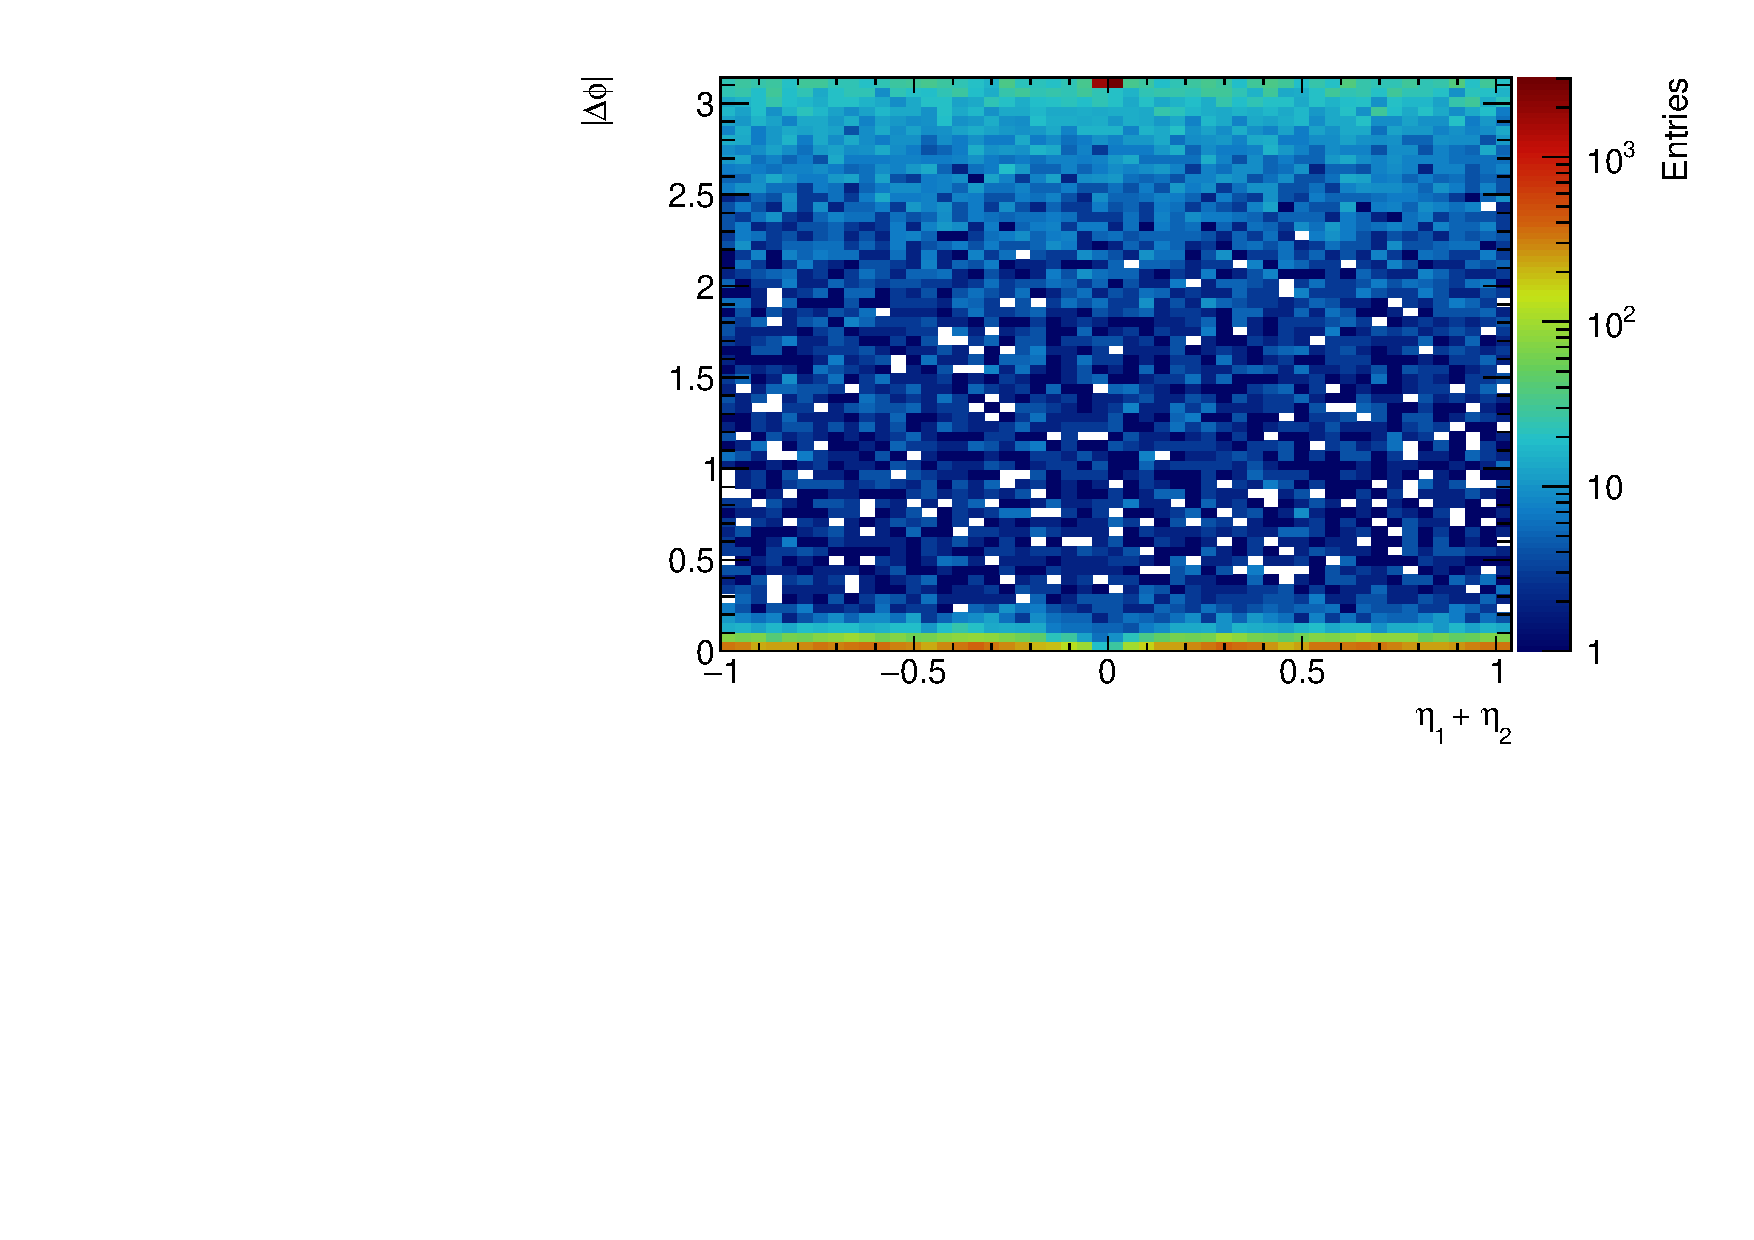
\includegraphics[width=0.6\textwidth]{figures/Cosmics/DataValidation/mup_seta_dphi.pdf}
    \label{fig:cosmicData}
    \caption{Distribution of pairs of two muons with highest $p_{T}$ in $|\Delta \phi|$ and $\eta_{1}+\eta_{2}$ found in the cosmic control region using the data sample. The sharp peak at $|\Delta\phi| = \pi$ and $\Sigma \eta = 0$ shows that a significant fraction of muon pairs in the region is from cosmic muons. The empty bins are shown with white.}
\end{center}
\end{figure}

To estimate the cosmic background in the signal region, the \Rcr distribution of \mumu pairs is compared to those forming a vertex in Figure~\ref{fig:cosmicCRb}. There are 246 \mumu vertices found in the data sample that pass all of the signal selection except the cosmic veto, and there is no event with \Rcr > 0.004, indicating that the cosmic background is effectively suppressed by the cosmic veto of \Rcr = 0.01.

The \Rcr distribution, normalized to \mumu pairs forming a vertex, yields a cosmic background of 0.27$\pm$0.14 (stat.). This background is about two orders of magnitude larger than the random-crossing background to be discussed. Therefore, the cosmic muon background is the dominant source of background in the signal region.


\begin{figure}[!htb]
    \centering
    \subfloat[Unscaled\label{fig:cosmicCRa}]{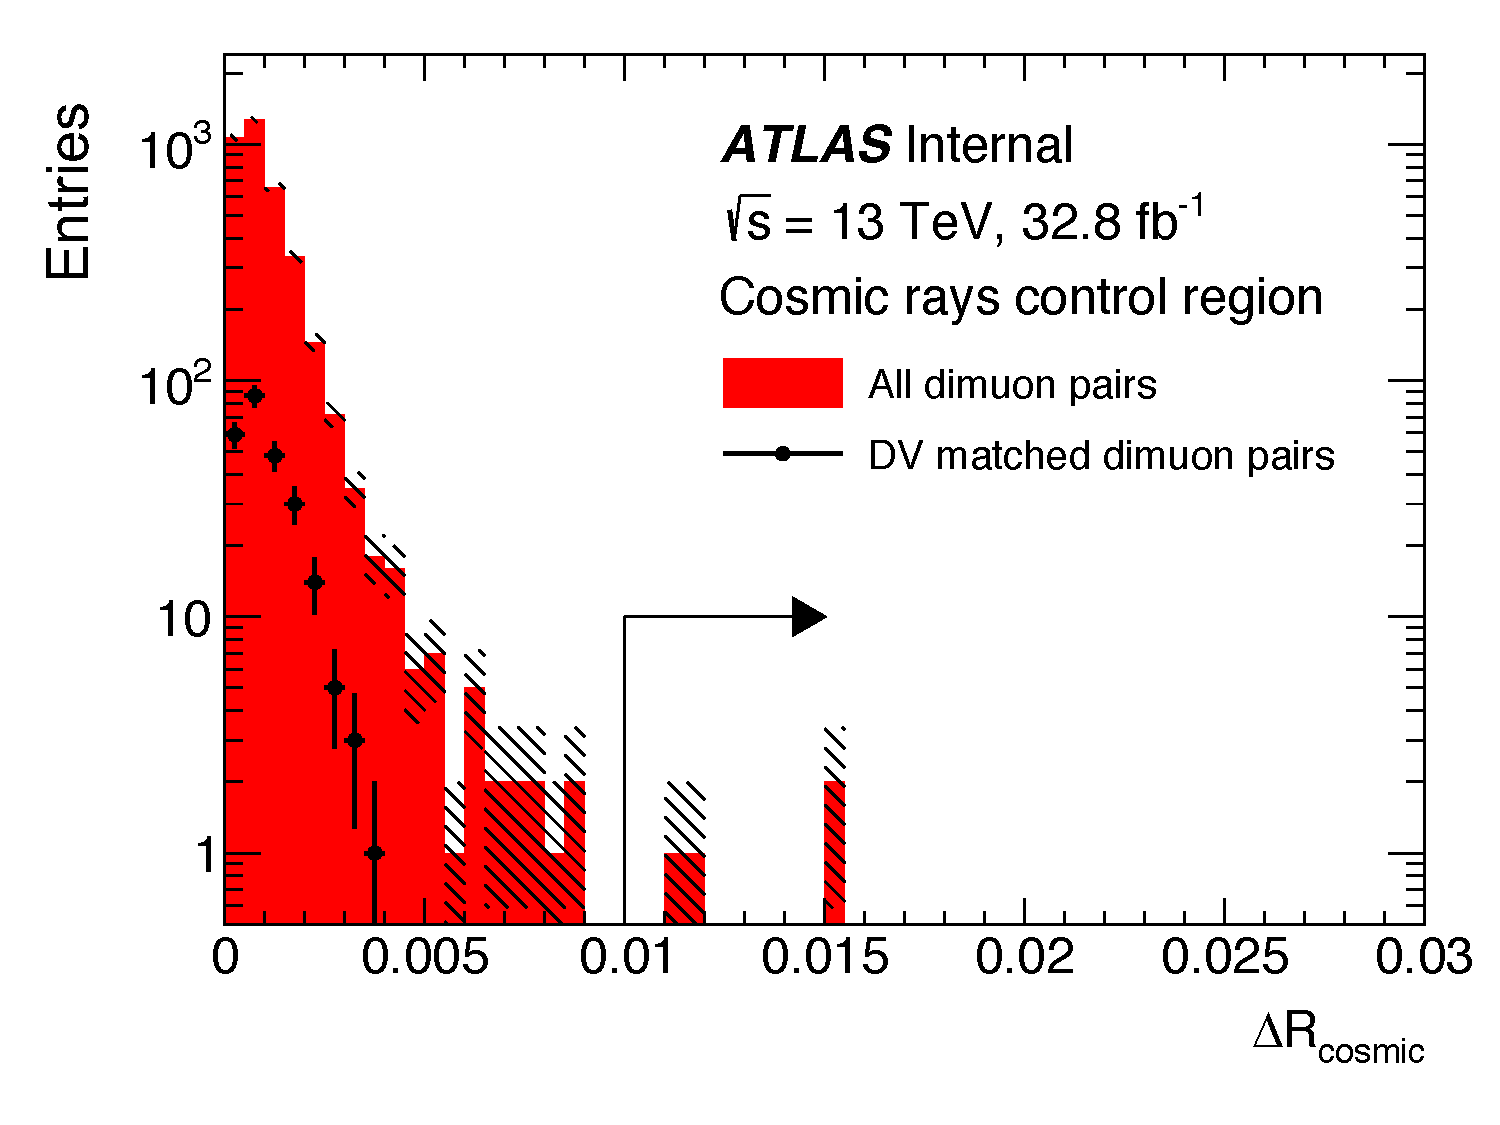
\includegraphics[width = 0.49 \textwidth]{figures/Cosmics/DataValidation/cosmics_unscaled.pdf}}
    \subfloat[Scaled\label{fig:cosmicCRb}]{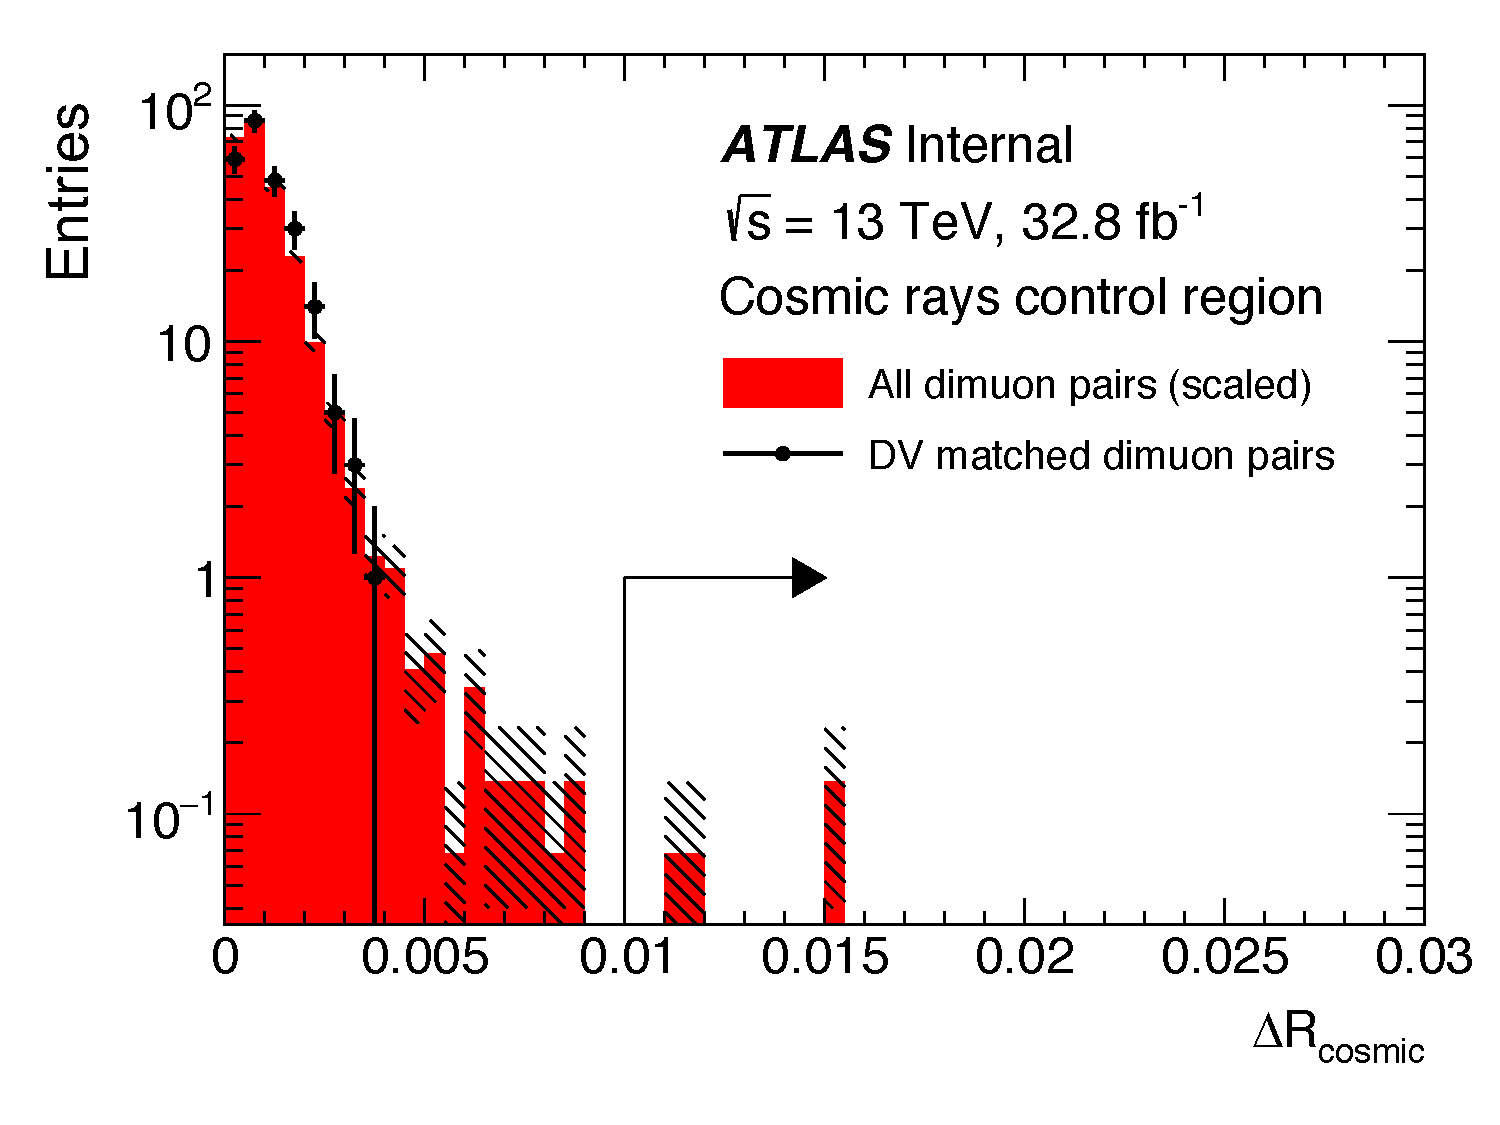
\includegraphics[width = 0.49 \textwidth]{figures/Cosmics/DataValidation/cosmics_scaled.pdf}}
    \label{fig:cosmicCR} 
	\caption{Comparison of the \Rcr distribution of \mumu pairs with (dots) and without (shaded) the vertex requirement. The same distribution is shown in (b) normalized to the number of \mumu pairs forming a vertex.}
	%\caption{(a) Distribution of \mumu vertices and pairs from the data sample in small \Rcr region. The red distribution represents all \mumu pairs. The black dots represent the subset of pairs forming a \mumu vertex. The same distribution is shown in (b) with \mumu pairs normalized to \mumu vertices.}
\end{figure}



\section{Random-Crossing Background}
\label{sec:bkg:random}

The random-crossing of two uncorrelated tracks can be a major source of the background in the search for displaced dilepton vertices. This background is expected to increase with more pile up in Run 2.
 
This random-crossing background is estimated by a data-driven method called the \textit{track flipping} (TF). In this method, secondary vertex reconstruction is performed on each pair of tracks from all possible combinations of tracks after one random track from each pair is flipped with respect to the beam spot. Because one track is flipped in each pair of tracks, the resulting vertices provide a good estimate for random-crossing background. In addition, another random-crossing background method, called \textit{event mixing}, is used to estimate systematic uncertainty in the background estimate.

The TF and event mixing methods are described in Section~\ref{sec:bkg:random_crossing_tf} and ~\ref{sec:bkg:random_crossing_em}, respectively. In Section~\ref{sec:bkg:random_crossing_MC}, the TF method is tested on the background MC samples, and the result is compared with the corresponding result from the event mixing. In Section~\ref{sec:bkg:random_crossing_data}, the random-crossing background in data is estimated by the TF method.%, and its systematic uncertainty is estimated by comparing the estimation from the TF and event mixing in Section~\ref{sec:bkg:random_crossing_syst}.

\subsection{Track Flipping Method}
\label{sec:bkg:random_crossing_tf}

In the TF method, events are selected by the same requirement described in Section~\ref{sec:selection:pre}. From the selected events, ID tracks associated with a muon, electron, or neither, referred as muon, electron, or non-leptonic track, respectively, are selected with the track criteria (Table~\ref{table:vertex_track_selection_simple}) used for the secondary vertexing algorithm. Lepton tracks are required to pass the same selection criteria described in Table~\ref{table:lepton_requirement}. Non-leptonic tracks are required to pass the same kinematic selection ($p_{T} > 10$ GeV, $|\eta| < $ 2.5) as leptons.

\begin{figure}[!htb]
    \subfloat[]{\label{subfig:TF_diagram_a}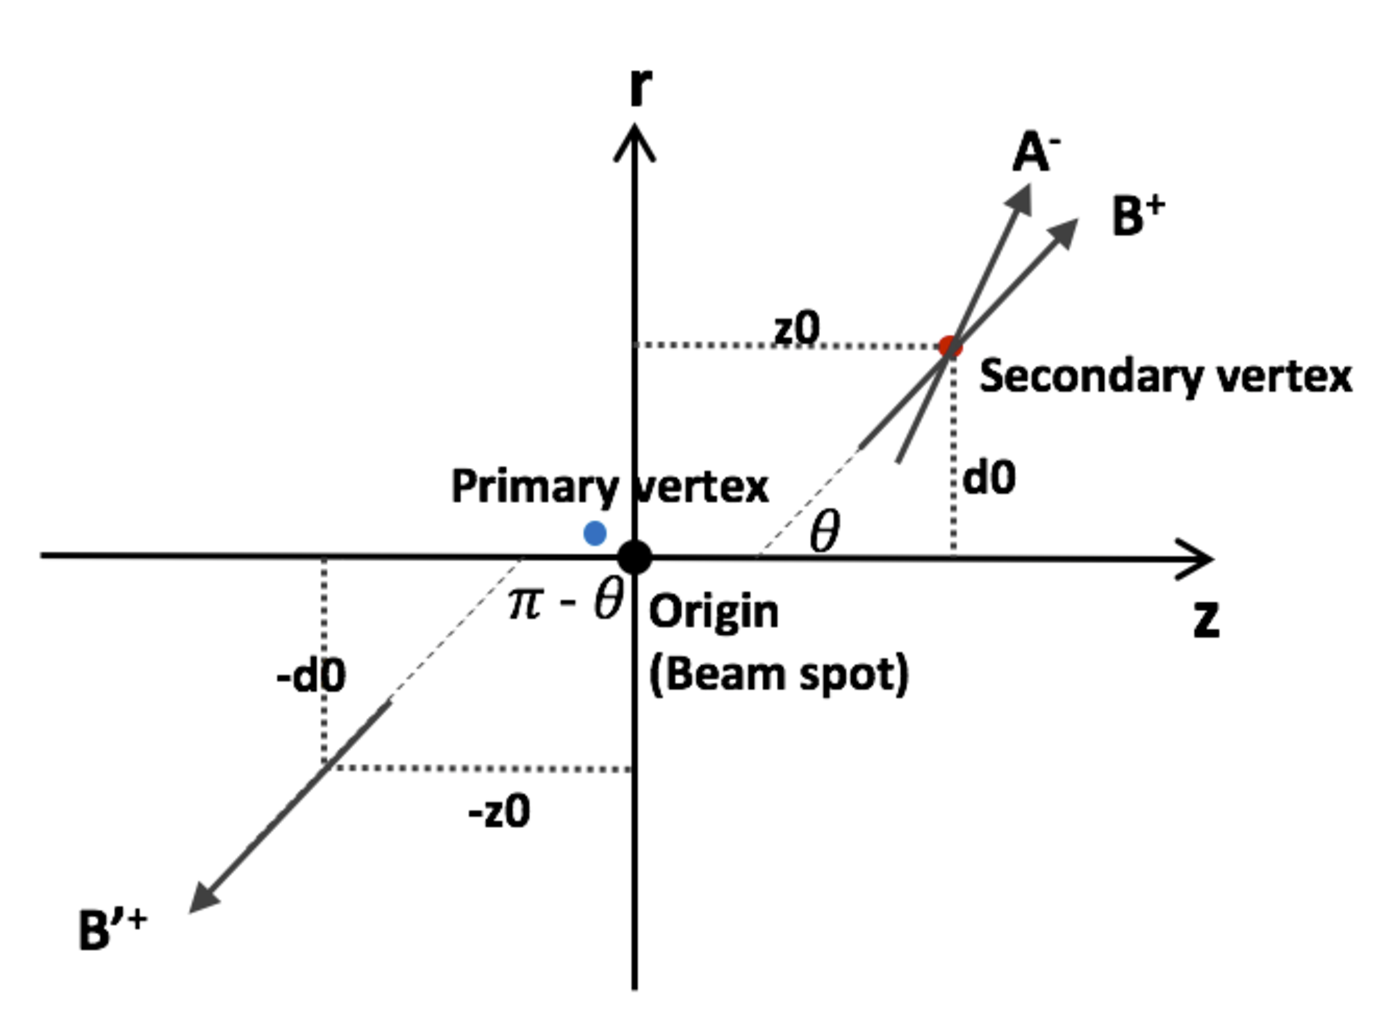
\includegraphics[width=0.50\textwidth]{figures/TF_diagram_a.pdf}}
    \subfloat[]{\label{subfig:TF_diagram_a}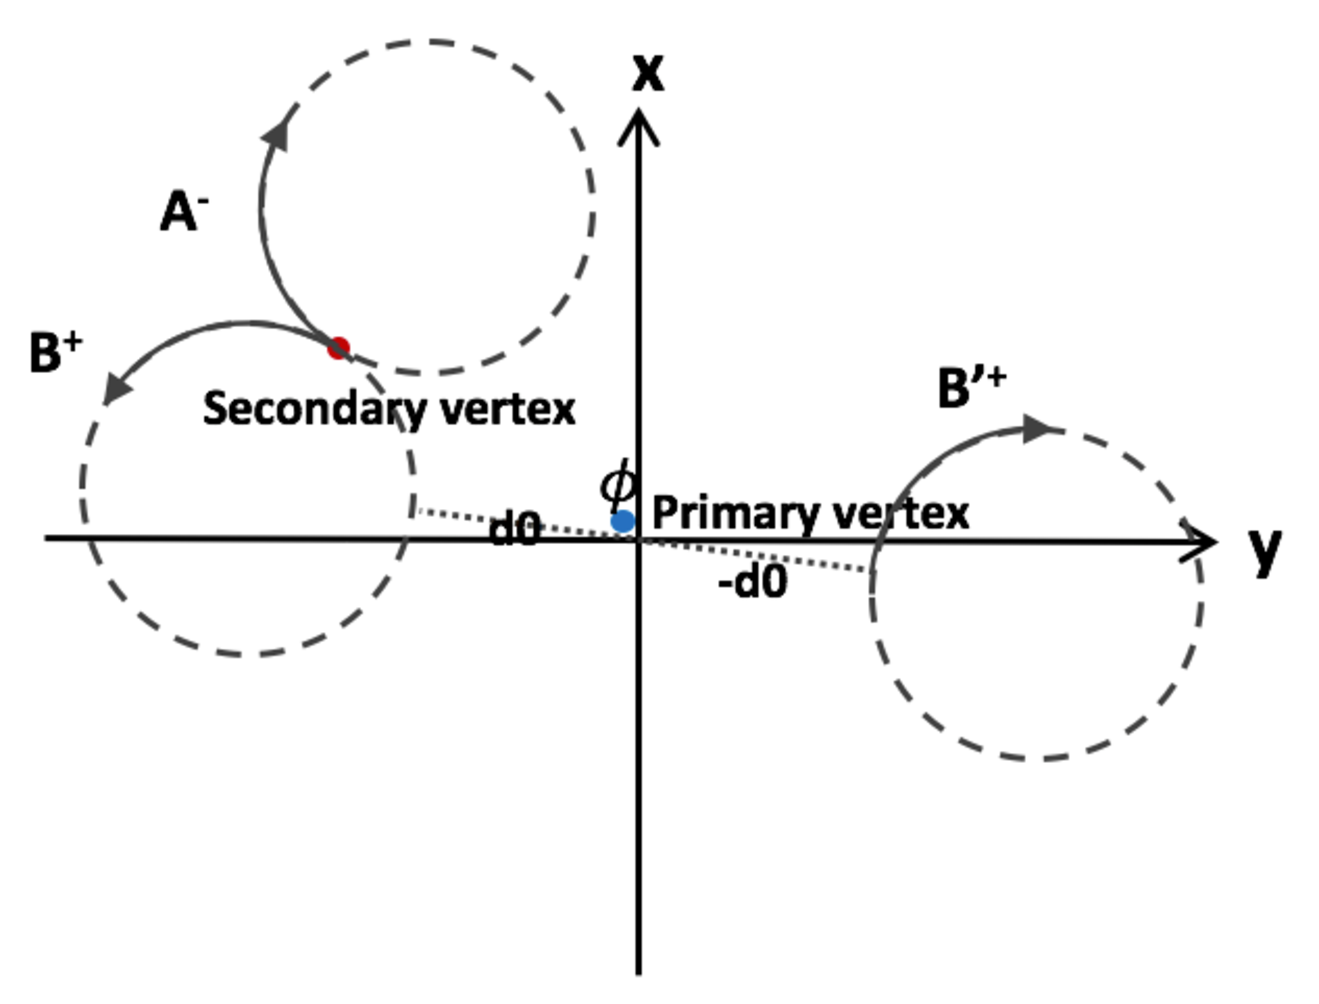
\includegraphics[width=0.50\textwidth]{figures/TF_diagram_b.pdf}}
	\centering
	\caption{Description of track flipping method in (a) $r-z$ and (b) $x-y$ plane. Given two tracks $A$ and $B$ originating from a common secondary vertex, one random track is flipped with respect to the beam spot and is denoted as $B'$. The resulting flipped track pair, $AB'$, cannot form a vertex due to the separation in space.}
	\label{fig:TF_diagram}
\end{figure}

From the selected tracks, track pairs are created from all possible combinations of muon, electron, or non-leptonic tracks, i.e. \mumu, \ee, \emu, \ex, \mux, or \xx, where x represents a non-leptonic track. For each pair of tracks, one random track is flipped with respect to the beam spot ($\dzero \rightarrow -\dzero, \zzero \rightarrow -\zzero, \phi\rightarrow\phi+\pi, \theta\rightarrow\pi-\theta$), creating a \textit{flipped track pair}. The secondary vertex algorithm used in the reconstruction of data or MC sample is used to reconstruct displaced vertices using these flipped track pairs. Vertex selection cuts similar to the cuts listed in Table~\ref{table:vertex_track_selection_simple} are applied to the vertices found from flipped track pairs, except that the trigger matching and filter matching are only required for $\mu\mu$, $ee$, and $e\mu$. 

Track-flipped vertices are formed purely from random-crossing of tracks as depicted in Figure~\ref{fig:TF_diagram}. Therefore, track-flipped vertex yields provide a good estimate for the random-crossing background. Also, because trigger and filter matchings are not imposed in the control and validation region, the TF method provides a conservative background estimation. 



\subsection{Event Mixing Method}
\label{sec:bkg:random_crossing_em}

The event mixing method is similar to the TF, but instead of flipping a track from a pair of tracks, it combines tracks from different events to create uncorrelated track pairs, i.e. two tracks do not originate from a real vertex.

The event mixing method proceed as follows. First, muon, electron, and non-leptonic tracks that satisfy the track criteria (Table~\ref{table:vertex_track_selection_simple}) are collected from all events, resulting in a collection of all potential seed objects in the sample. Lepton tracks are required to pass the same selection criteria\footnote{Only lepton pairs with an invariant mass greater than $6~\si{\GeV}$ are used in the normalization procedure to remove any contamination from low mass processes.} described in Table~\ref{table:lepton_requirement}. Non-leptonic tracks are required to pass the minimal kinematic selection ($p_{T} > 10$ GeV, $|\eta| <$ 2.5 to match with the kinematic selection for leptons.

Pairs of tracks are randomly sampled from the collection. For each track pair, a primary vertex is randomly chosen from all events with a lepton candidate. Primary vertices are needed in order to evaluate the displacement cut and quality requirements of the vertexing algorithm. The secondary vertex reconstruction is performed on each track pair.

The ratio of event-mixing vertex yields to the number of track pairs sampled represents the probability, $p_{\mathrm{xing}}$, of two tracks randomly forming a displaced vertex. Using $p_{\mathrm{xing}}$ and the total number of track pairs of each type (\mumu, \ee, \emu, \mux, \ex, \xx) in data, the random-crossing background is estimated for each type by, e.g.,

\begin{equation}
    N_{\mumu}^{v} = N_{\mumu} \times p_{\mathrm{xing}},
\label{eq:N_Comb_Vertices}
\end{equation}
%
where $N_{\mumu}^{v}$ represent the estimated random-crossing background of \mumu type, and $N_{\mumu}$ represents the total number of \mumu pairs present in data. The random-crossing probability, $p_{\mathrm{xing}}$, is estimated individually for each type of vertices. The details on this method can be found in Ref.~\cite{DuarteCampderros:2275055}.







\subsection{MC Study}
\label{sec:bkg:random_crossing_MC}
The track-flipping and event mixing methods are compared using the background MC samples (Table~\ref{table:background_MC}). Similar event, track, and vertex selections are applied as the signal selection, but the track $p_{T}$ requirement is lowered to $p_{T} > 5$ GeV and opposite charge requirement is removed for more statistics. A representative plot of vertex cut flows in the TF method is shown in Figure~\ref{fig:m_FBE_cutflow_MC} using track-flipped \xx vertices from the background MC samples.

%The TF method is tested using the background MC sample (Table~\ref{table:background_MC}), and the resulting vertex yields and distributions are compared with the corresponding result from event mixing method. Similar event, track, and vertex selections are applied as the signal selection, but the track $p_{T}$ requirement is lowered to $p_{T} > 5$ GeV and opposite charge requirement is removed for more statistics. A representative plot of vertex cut flows in the TF method is shown in Figure~\ref{fig:m_FBE_cutflow_MC} using track-flipped \xx vertices from the background MC samples.

\begin{figure}[!htb]
	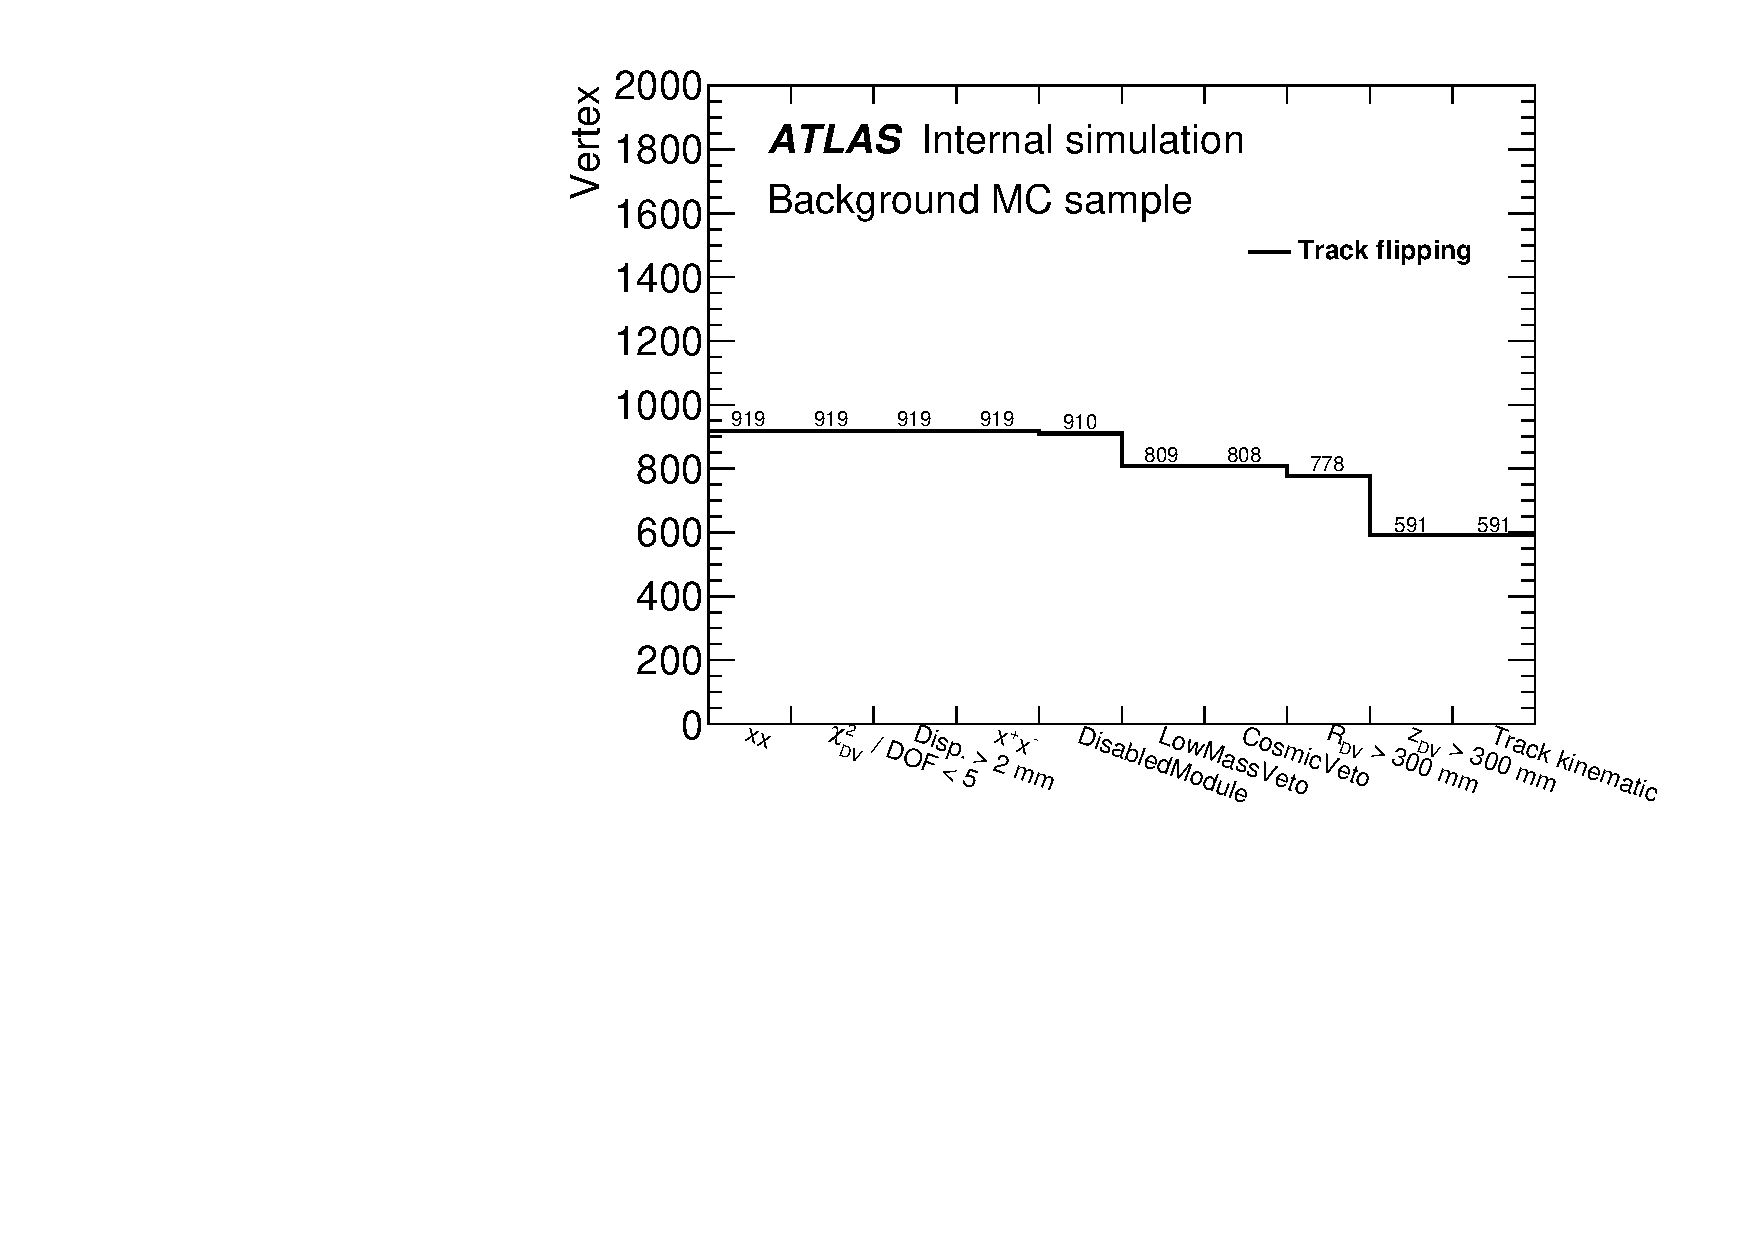
\includegraphics[width=0.60\textwidth]{figures/m_FBE_cutflow_MC.pdf}
	\centering
	\caption{Vertex cut flow applied on \xx vertices from the TF method.}
	\label{fig:m_FBE_cutflow_MC}
\end{figure}

The vertex yields from the TF and event mixing method, which represent the estimation for random-crossing background, are compared with the vertex yields from reconstruction in Table~\ref{table:random_vertex_count}. No random-crossing background of \mumu, \ee, or \emu type is expected from the MC samples using both methods. 
 
\begin{table}[!htb]
  \centering
  \begin{tabular}{ c  c c c }
    \hline
    \hline
	Vertex Type					&Track flipping	    &   Event Mixing 	    & MC                    \\
    \hline
	$\mu$x						&	3			    &	4        			&	5					\\
	$e$x						&	5			    &	2   				&	4					\\
	xx						    &	1154		    &	1125 				&	989 				\\
    \hline
    \hline
  \end{tabular}
  \caption{Comparison of the estimated vertex yields from the TF and event mixing with those reconstructed in the background MC samples.}
  \label{table:random_vertex_count}
\end{table}

The vertex yields from the TF and the event mixing methods agree within the statistical uncertainty. The kinematic distributions of xx vertices in TF and event mixing are compared with those of the background MC samples in Figure~\ref{fig:random-crossing_vertex_dist}. Both samples reproduce the vertex distribution in the background MC samples.

\begin{figure}[!htb]
    \centering
    \subfloat[]{\label{subfig:random-crossing_MC_M}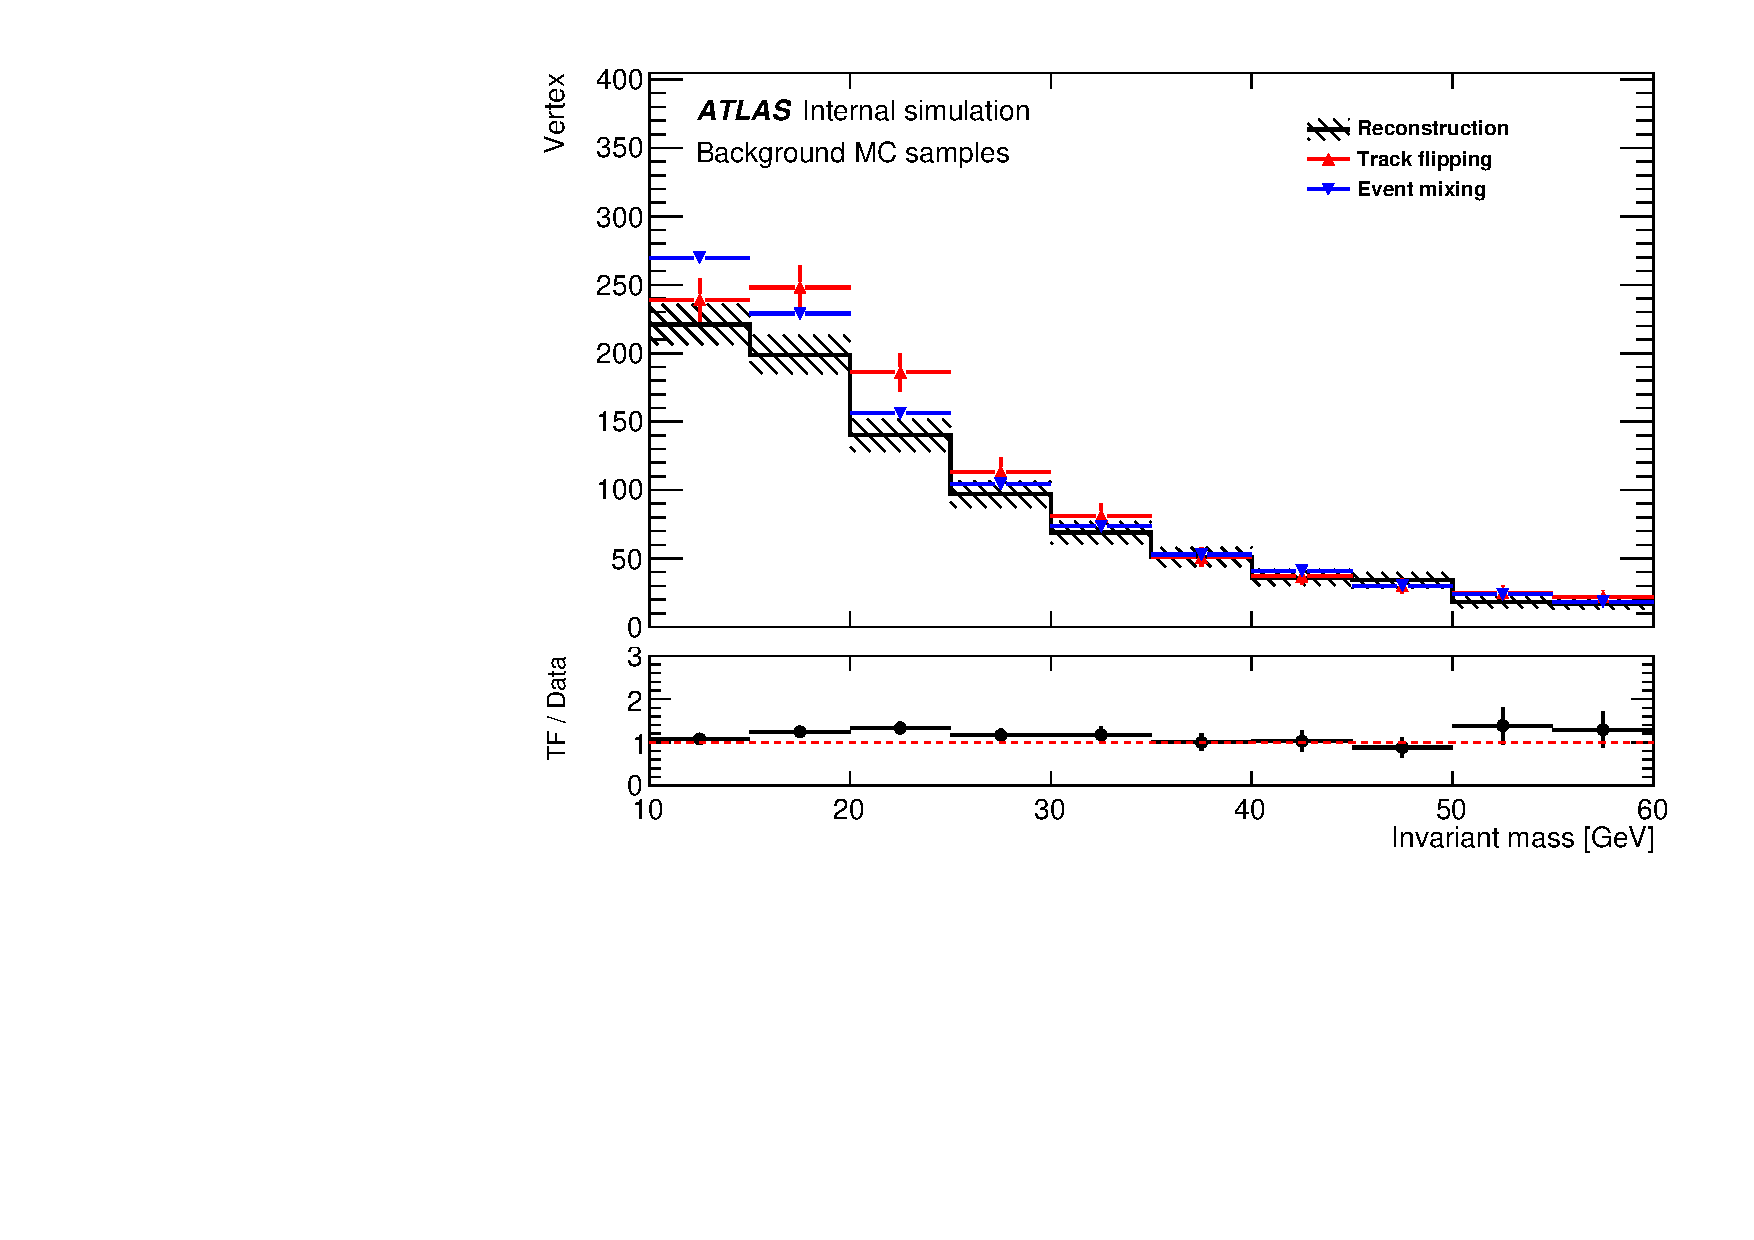
\includegraphics[width=0.45\textwidth]{figures/m_FBE_M.pdf}}
    \subfloat[]{\label{subfig:random-crossing_MC_chi2ndof}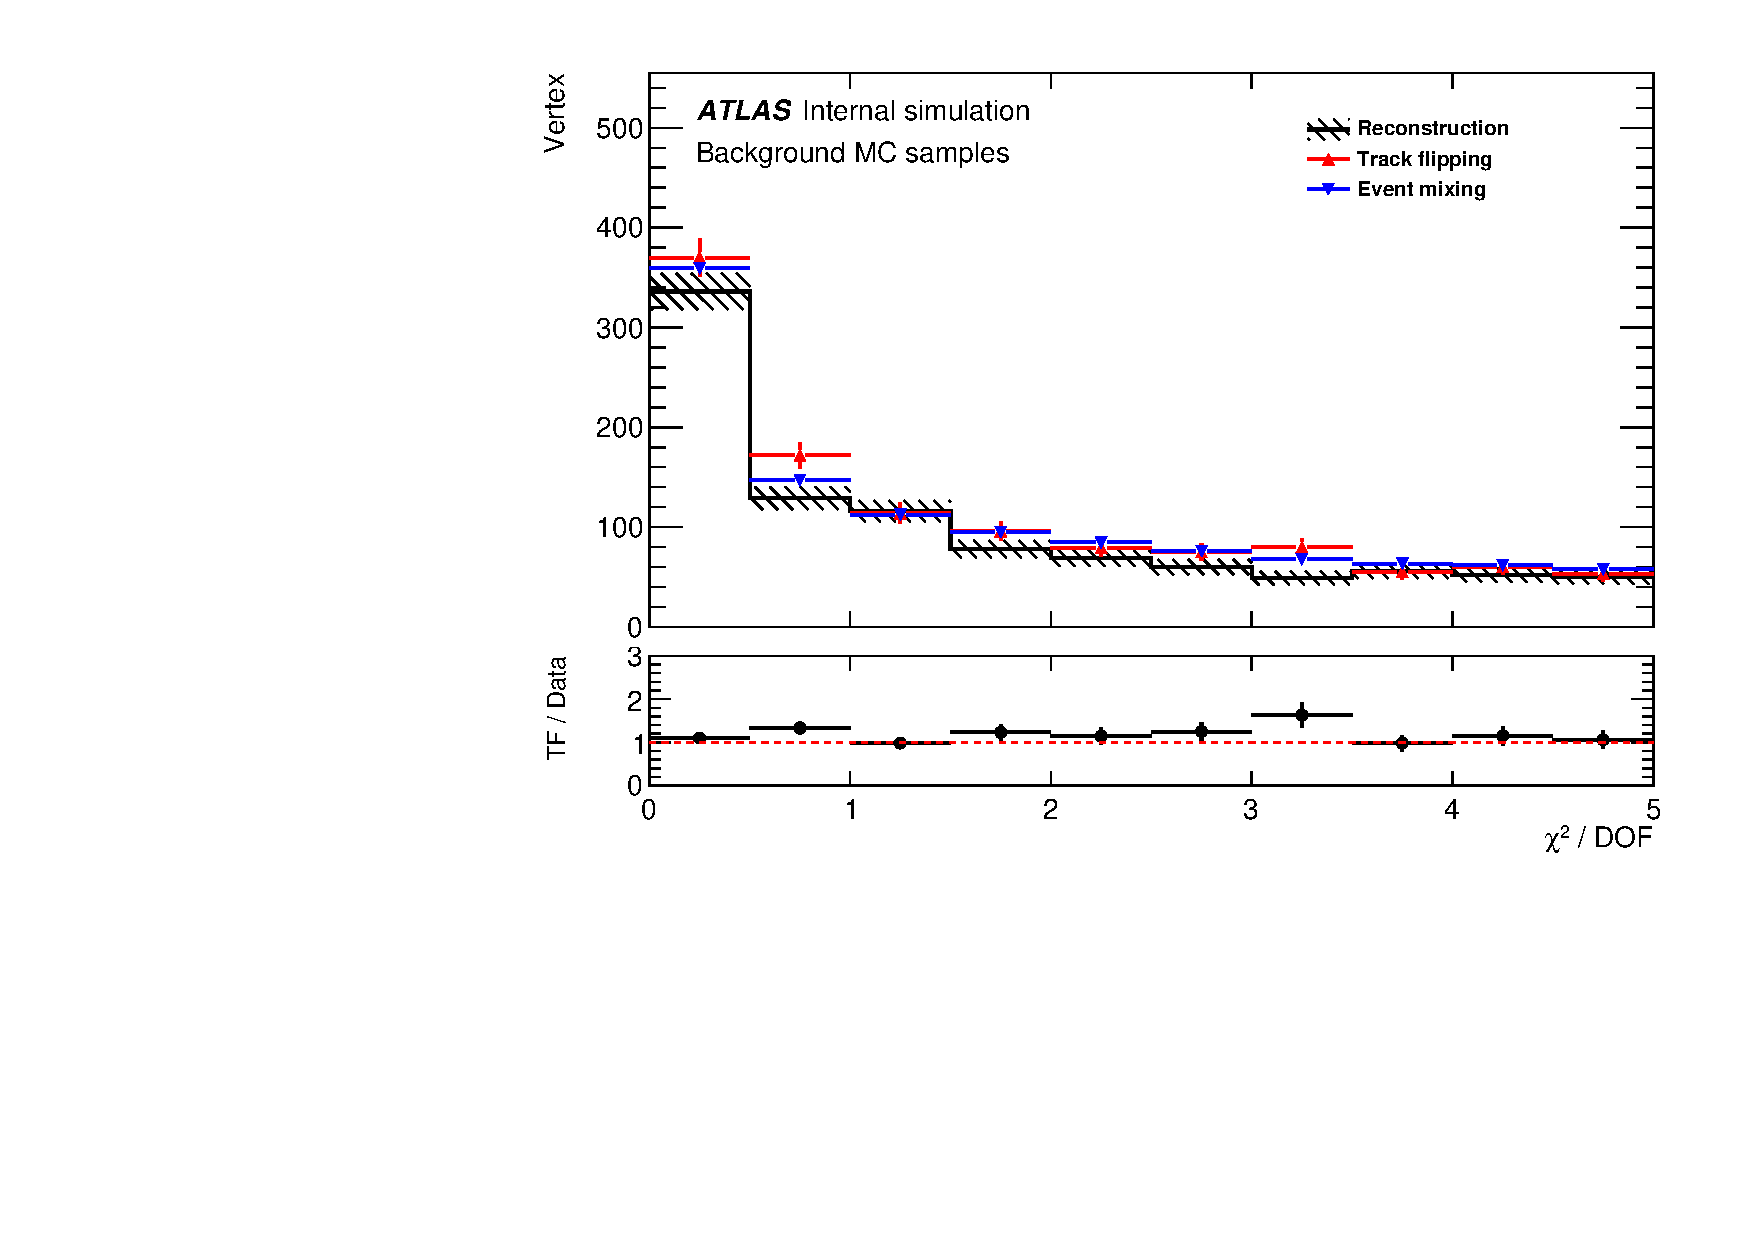
\includegraphics[width=0.45\textwidth]{figures/m_FBE_chi2_ndof.pdf}} \\
    \subfloat[]{\label{subfig:random-crossing_MC_r}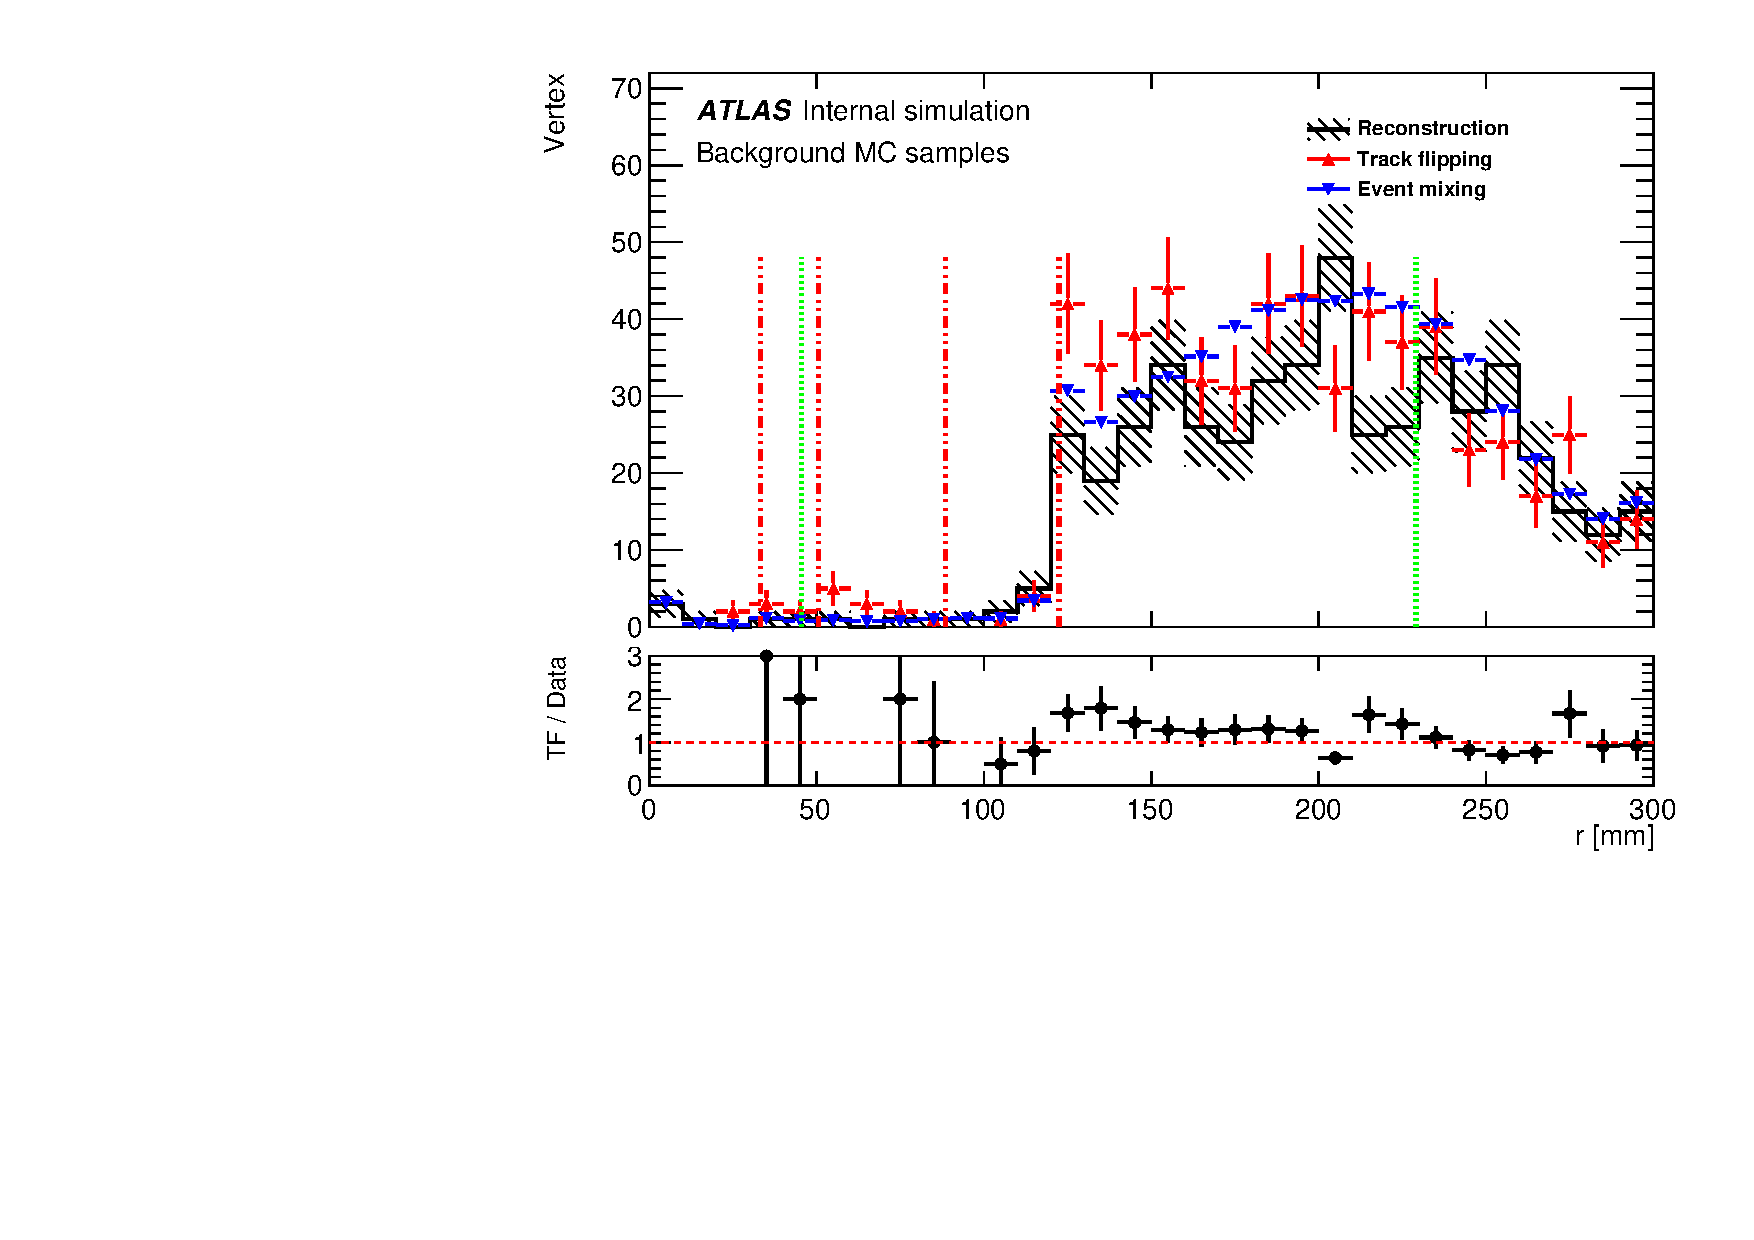
\includegraphics[width=0.45\textwidth]{figures/m_FBE_R.pdf}}
    \subfloat[]{\label{subfig:random-crossing_MC_z}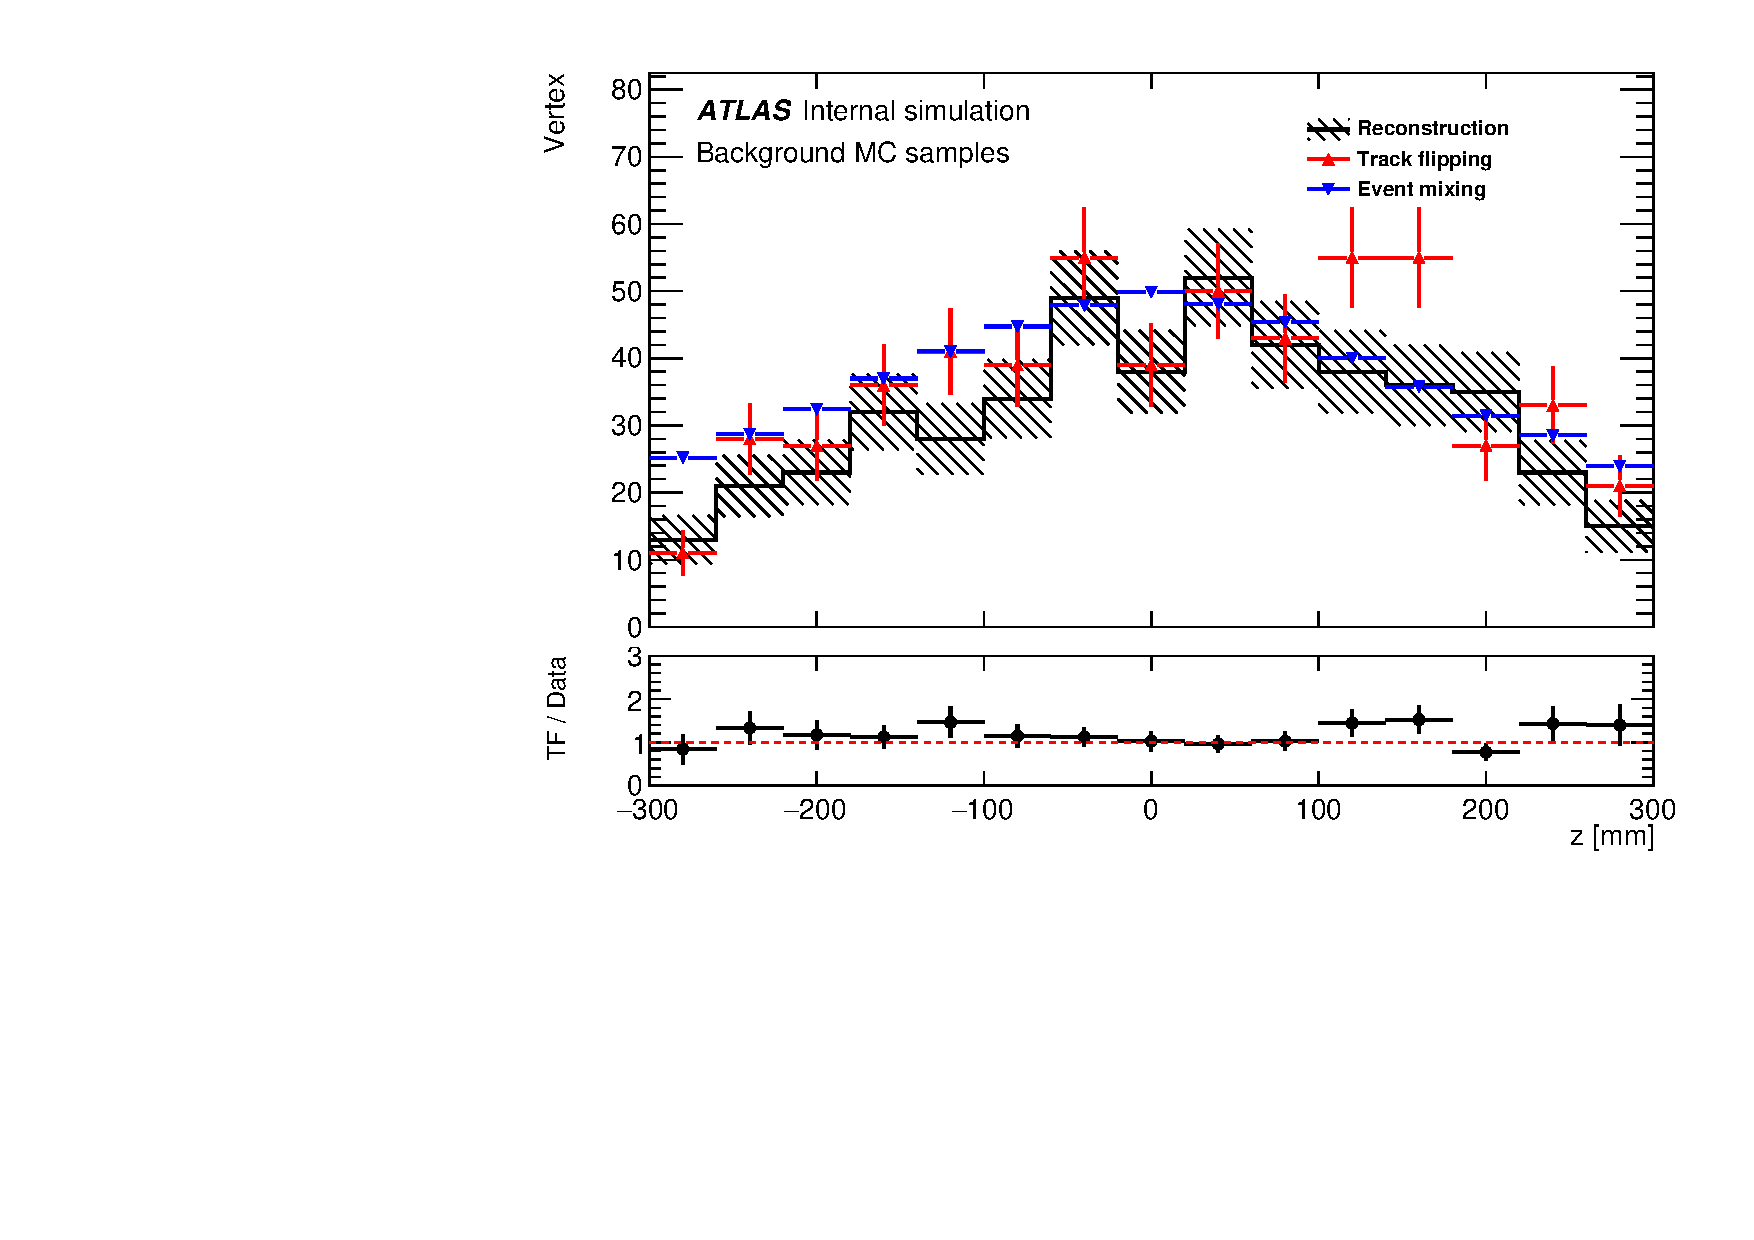
\includegraphics[width=0.45\textwidth]{figures/m_FBE_z.pdf}}
    %\subfloat[l]{\label{subfig:random-crossing_l}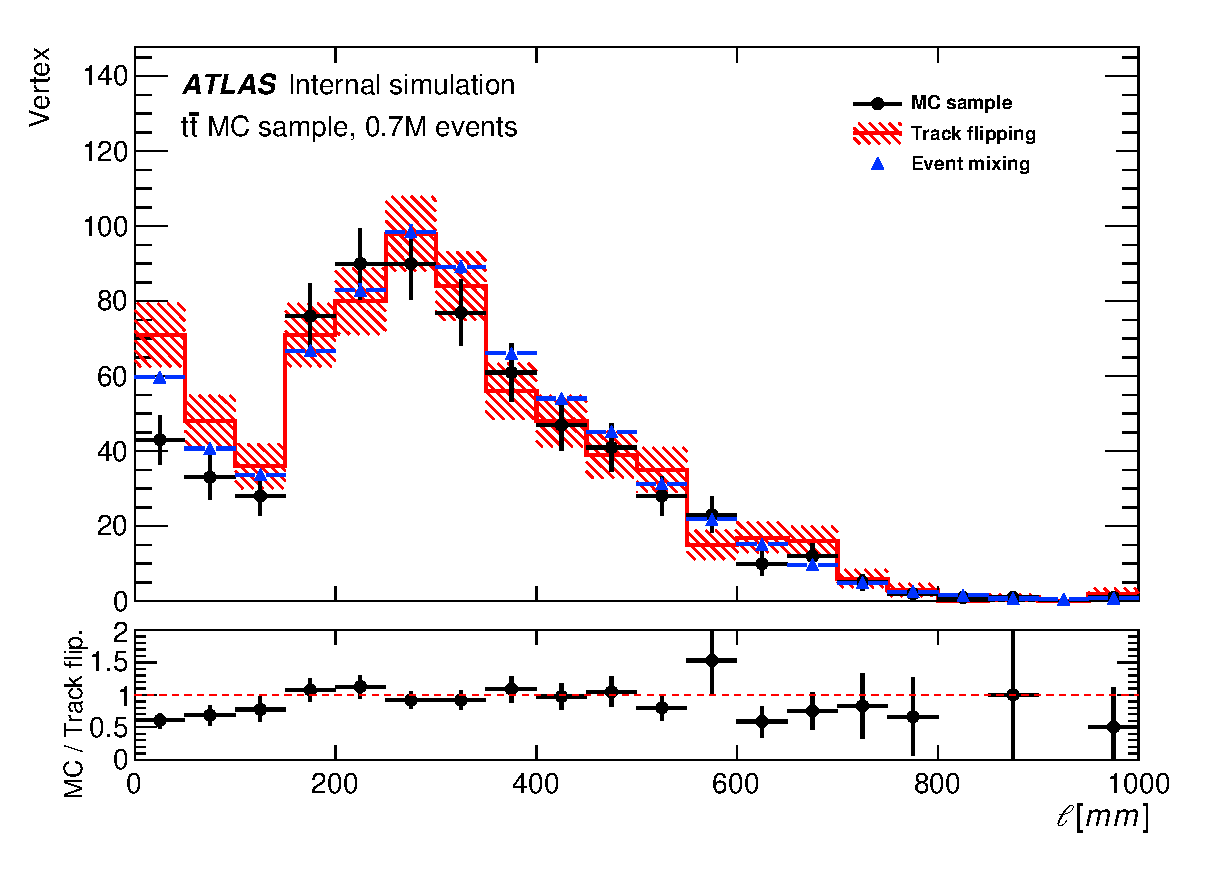
\includegraphics[width=0.45\textwidth]{figures/m_FBE_l.eps}}
    \caption{Comparison of (a) vertex mass, (b) $\chi^{2} / \mathrm{DOF}$, (c) transverse, and (d) longitudinal position of \xx vertices reconstructed in TF and event mixing with those reconstructed in the background MC samples. In (c), the red dashed lines indicate the four Pixel layers. The green dotted lines indicate the Inner Support Tube (45.5 mm) and Pixel Support Tube (229 mm).}
    \label{fig:random-crossing_vertex_dist}
\end{figure}


\subsection{Estimating Random-crossing Background with Data Sample}
\label{sec:bkg:random_crossing_data}

The random-crossing background is estimated by performing the TF method on the data sample. Following the procedure described in Section~\ref{sec:bkg:random_crossing_tf}, track-flipped vertices are created, and the vertex yields in the control and validation regions can be used to estimate the random-crossing background in the signal region.

In the control region, the xx vertices found from the track flipping method are compared to the vertices reconstructed in the data sample in Figure~\ref{fig:random-crossing_vertex_dist_data}. The distributions shows that the TF method reproduces the data reasonably well including some of the structures of the ID, suggesting that the TF method provides a reasonable estimation of the random-crossing background.

\begin{figure}[!htb]
    \centering
    \subfloat[]{\label{subfig:random-crossing_M}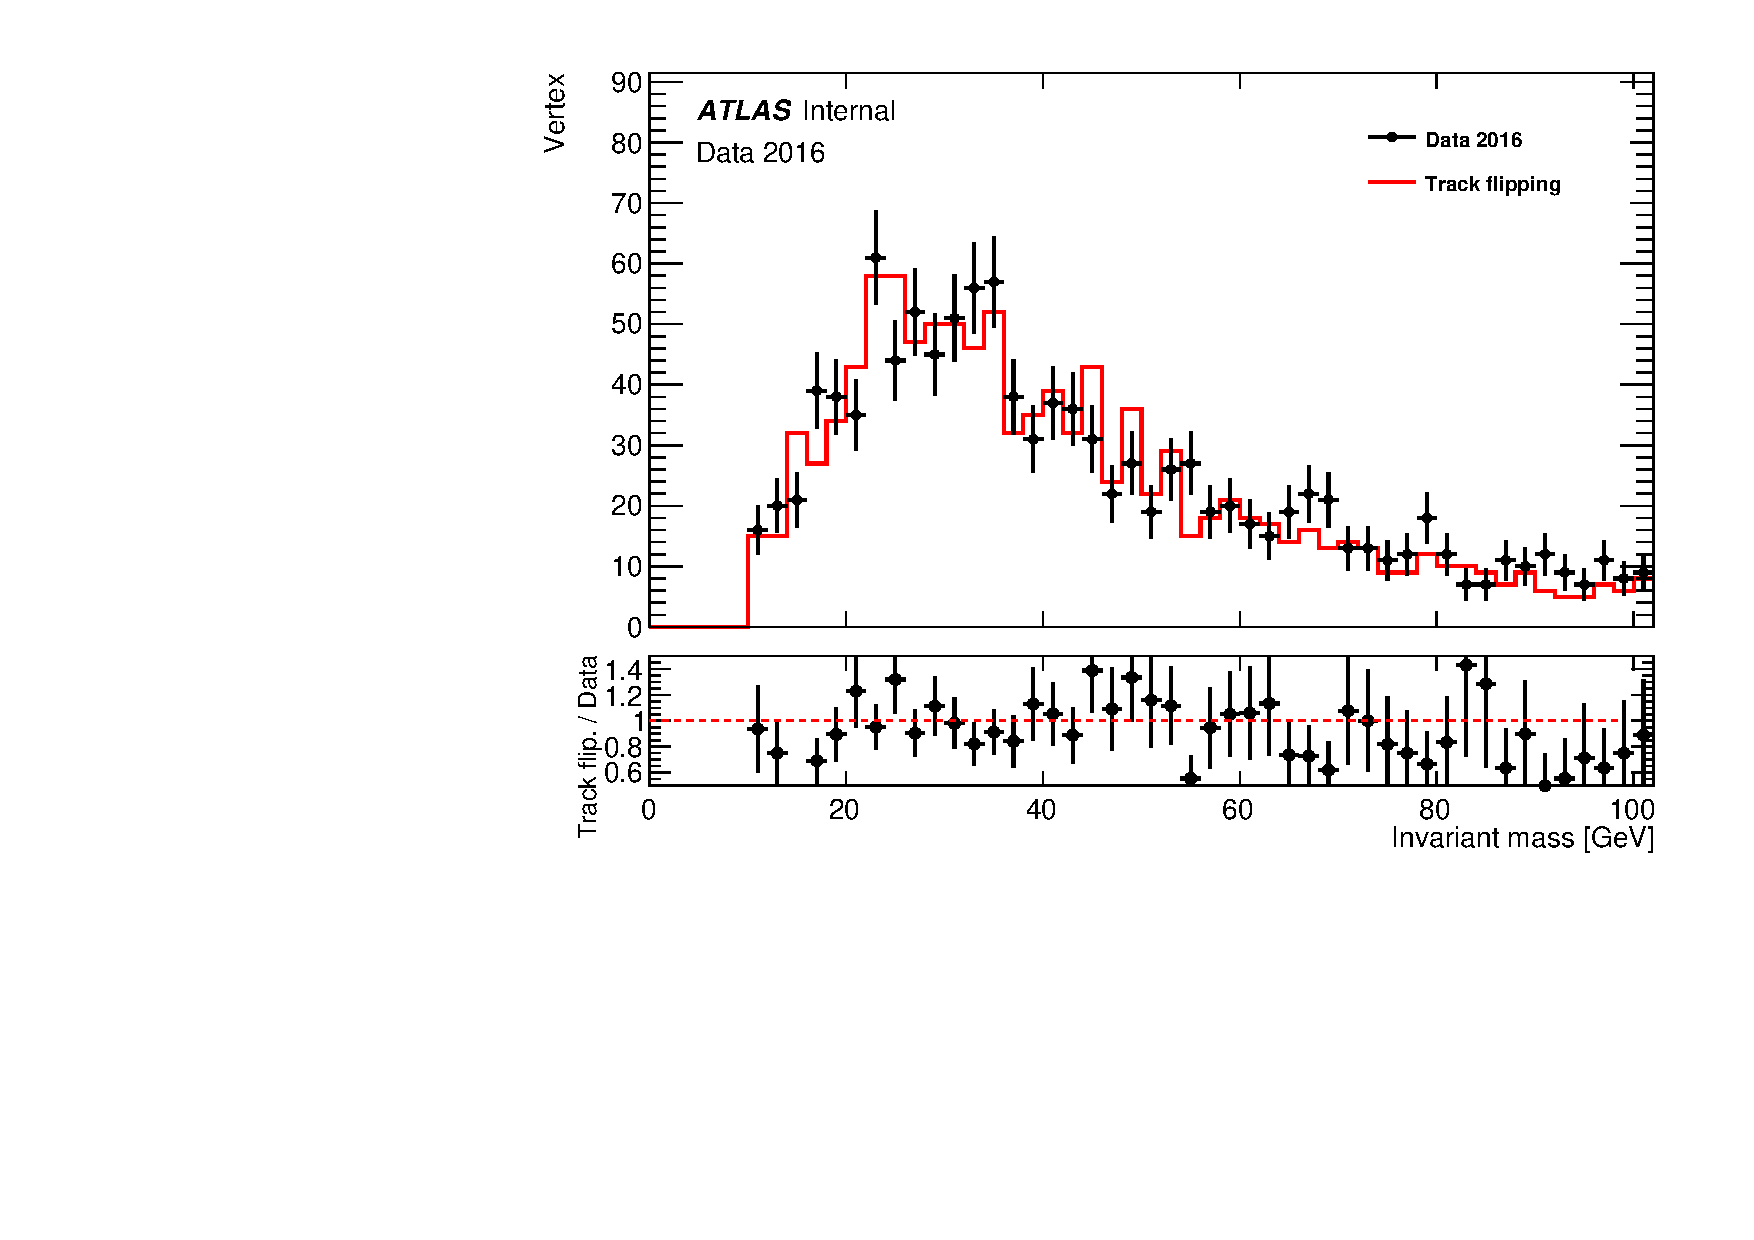
\includegraphics[width=0.45\textwidth]{figures/m_FBE_data_M.pdf}}
    \subfloat[]{\label{subfig:random-crossing_chi2ndof}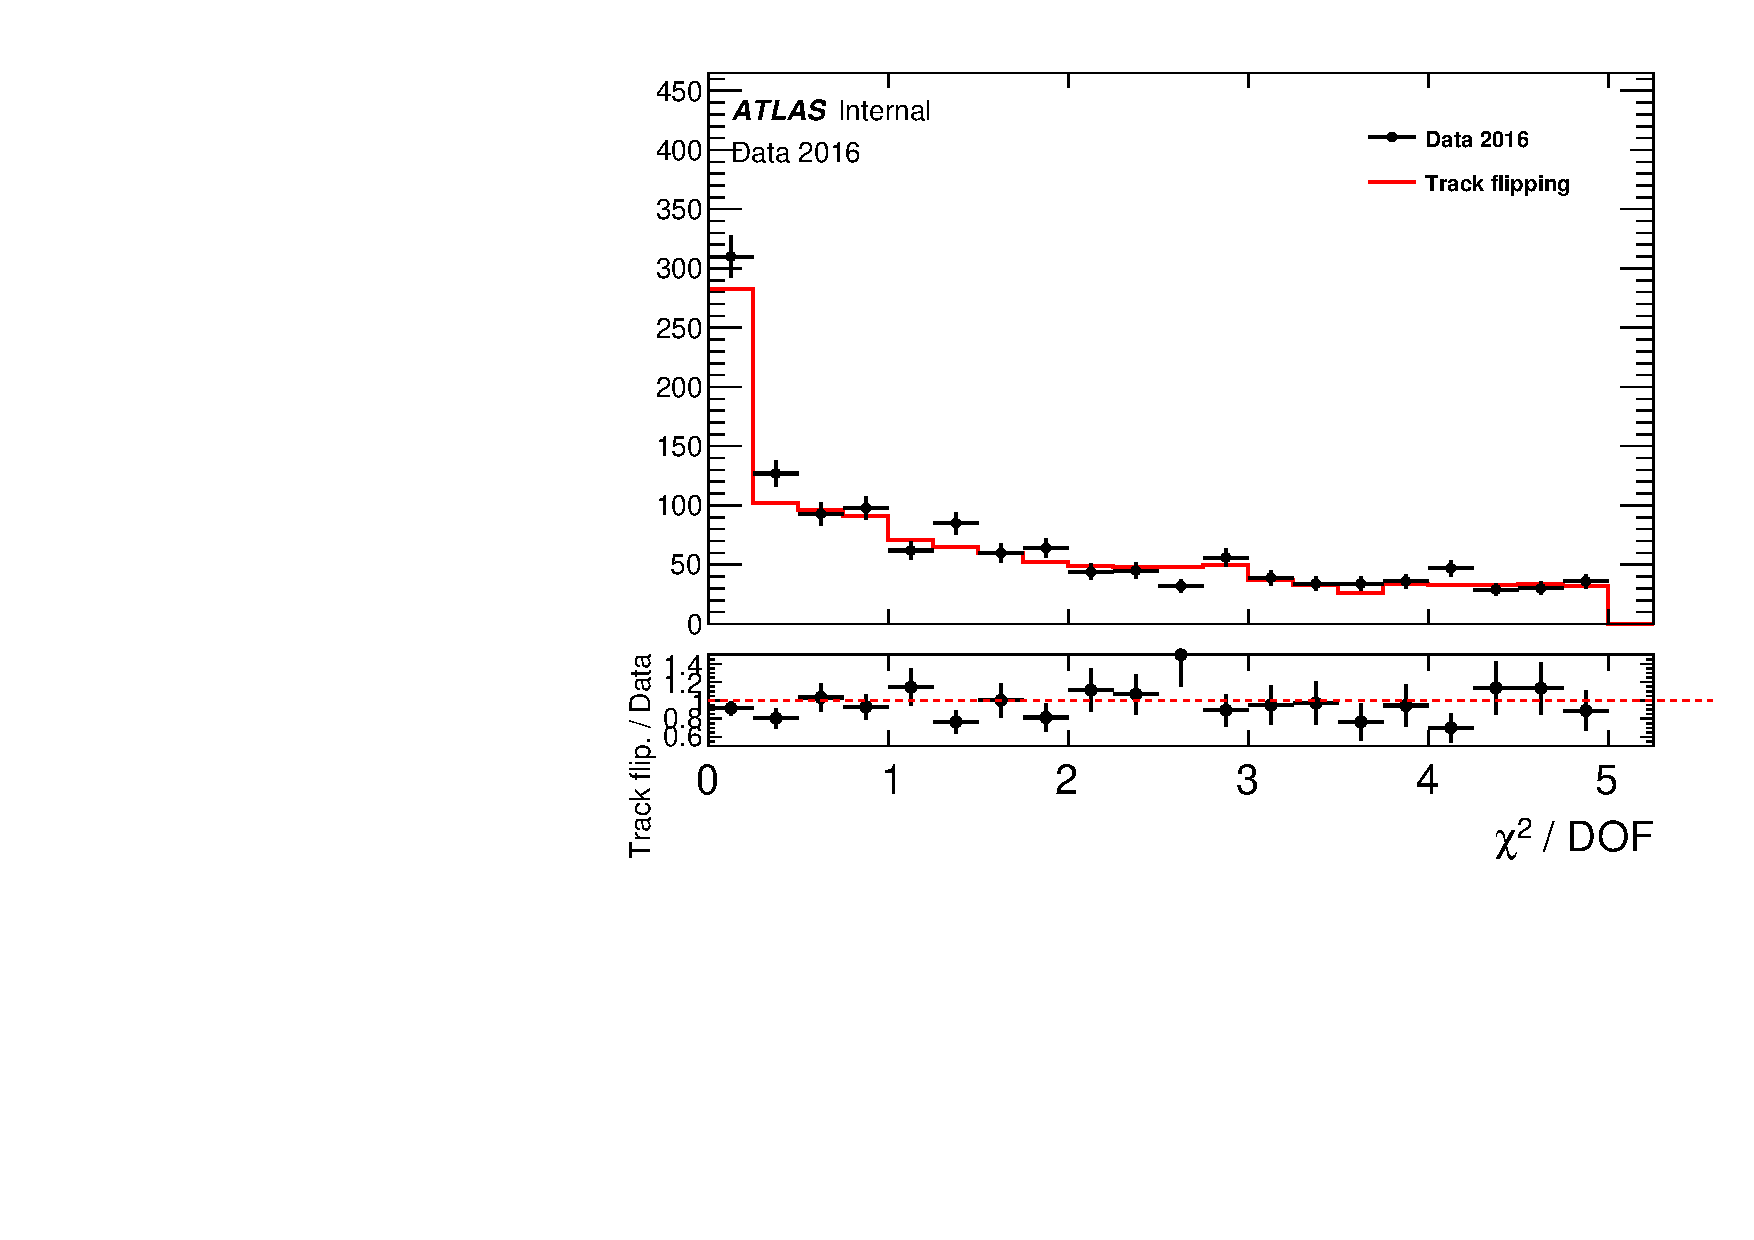
\includegraphics[width=0.45\textwidth]{figures/m_FBE_data_chi2_ndof.pdf}} \\
    \subfloat[]{\label{subfig:random-crossing_r}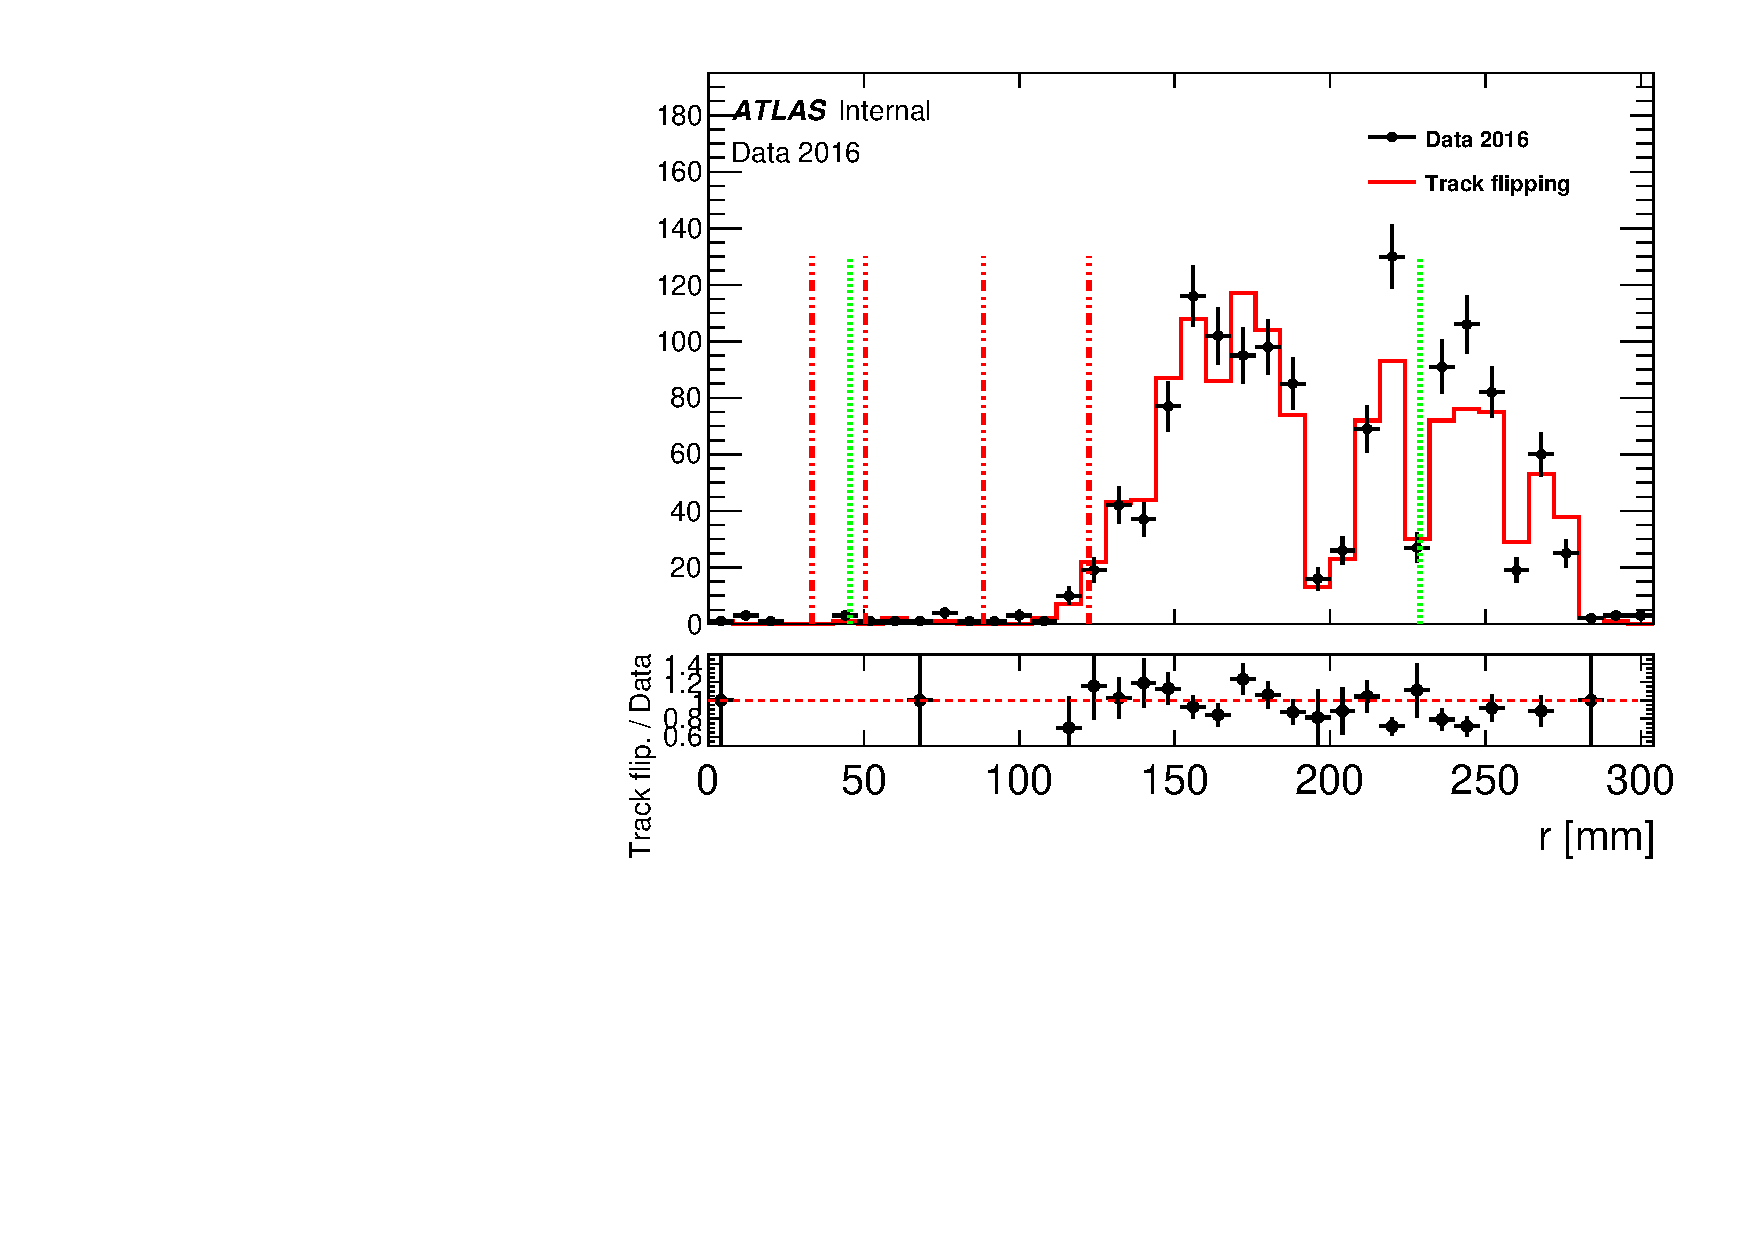
\includegraphics[width=0.45\textwidth]{figures/m_FBE_data_R.pdf}}
    \subfloat[]{\label{subfig:random-crossing_z}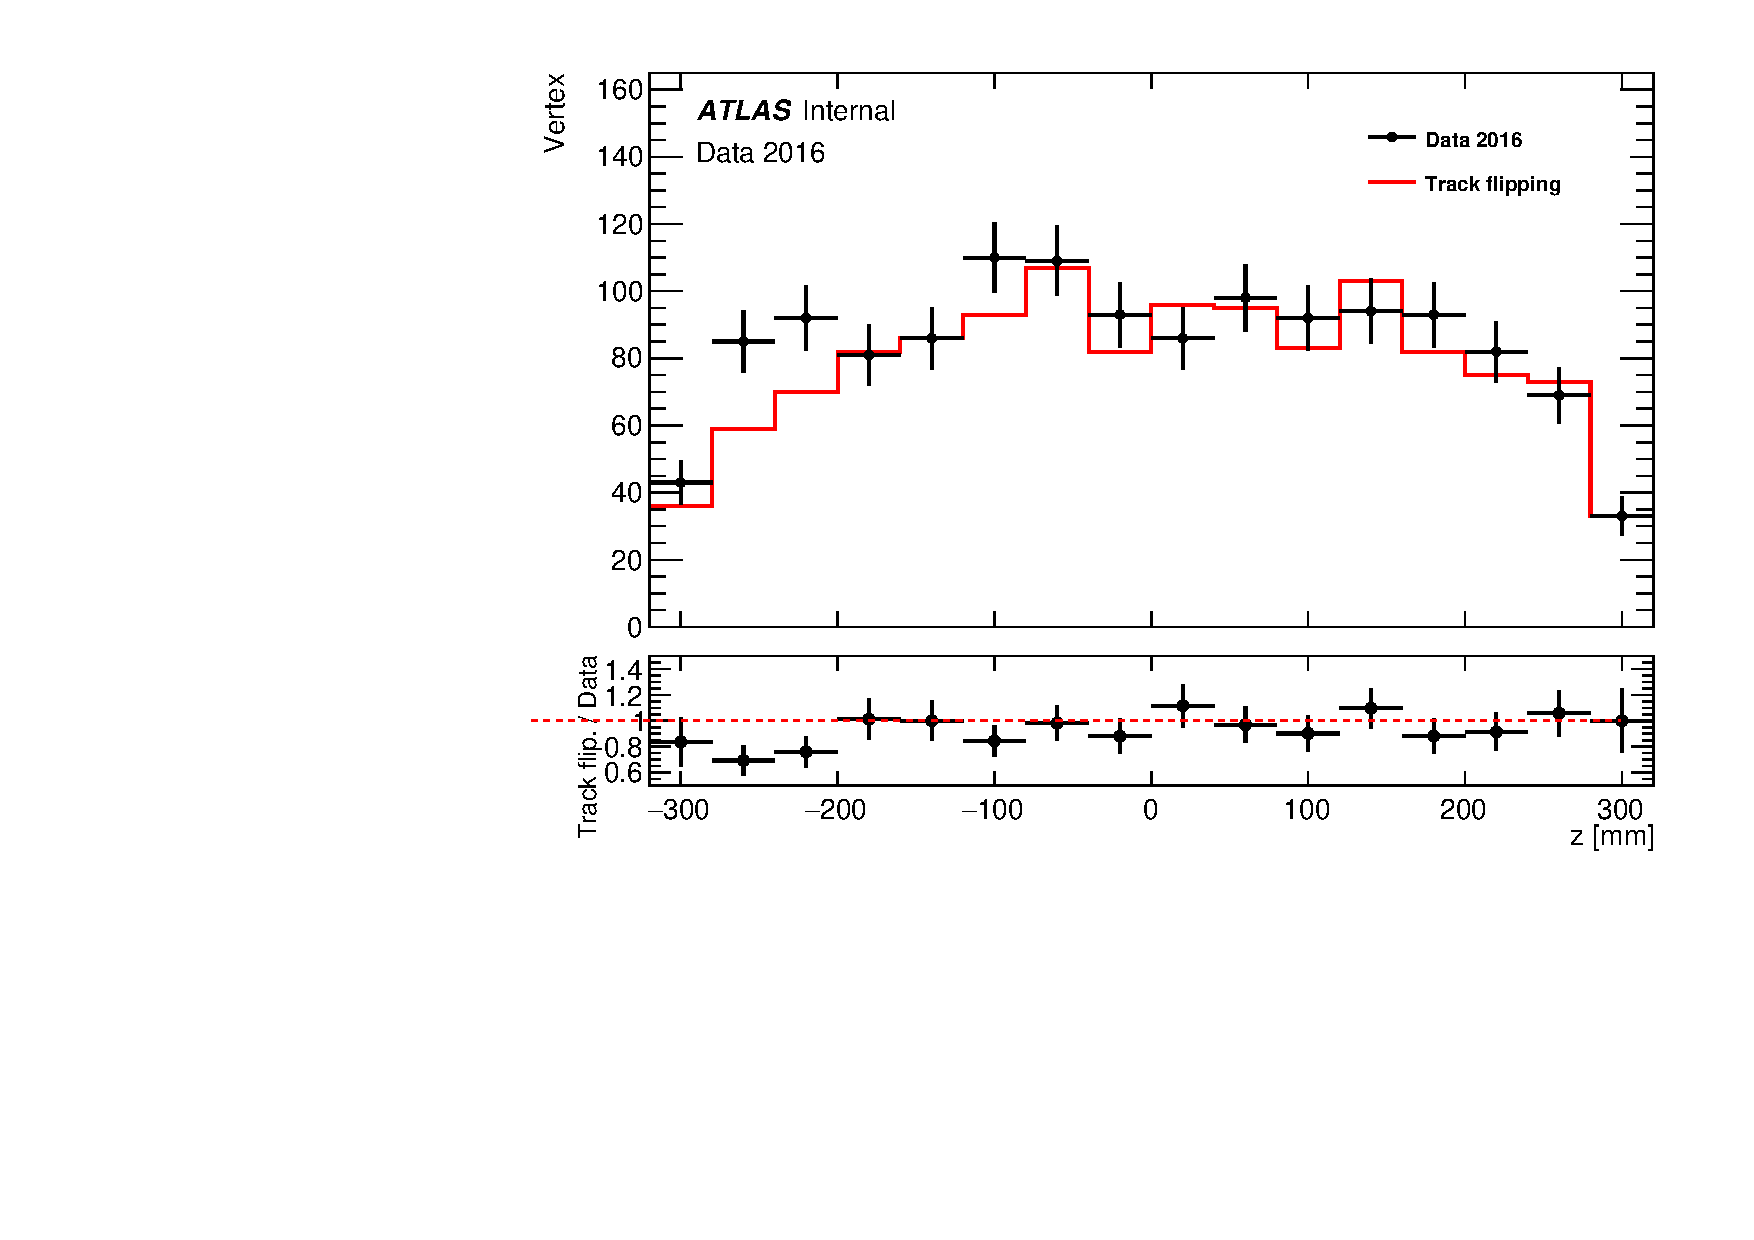
\includegraphics[width=0.45\textwidth]{figures/m_FBE_data_z.pdf}}
    %\subfloat[l]{\label{subfig:random-crossing_l}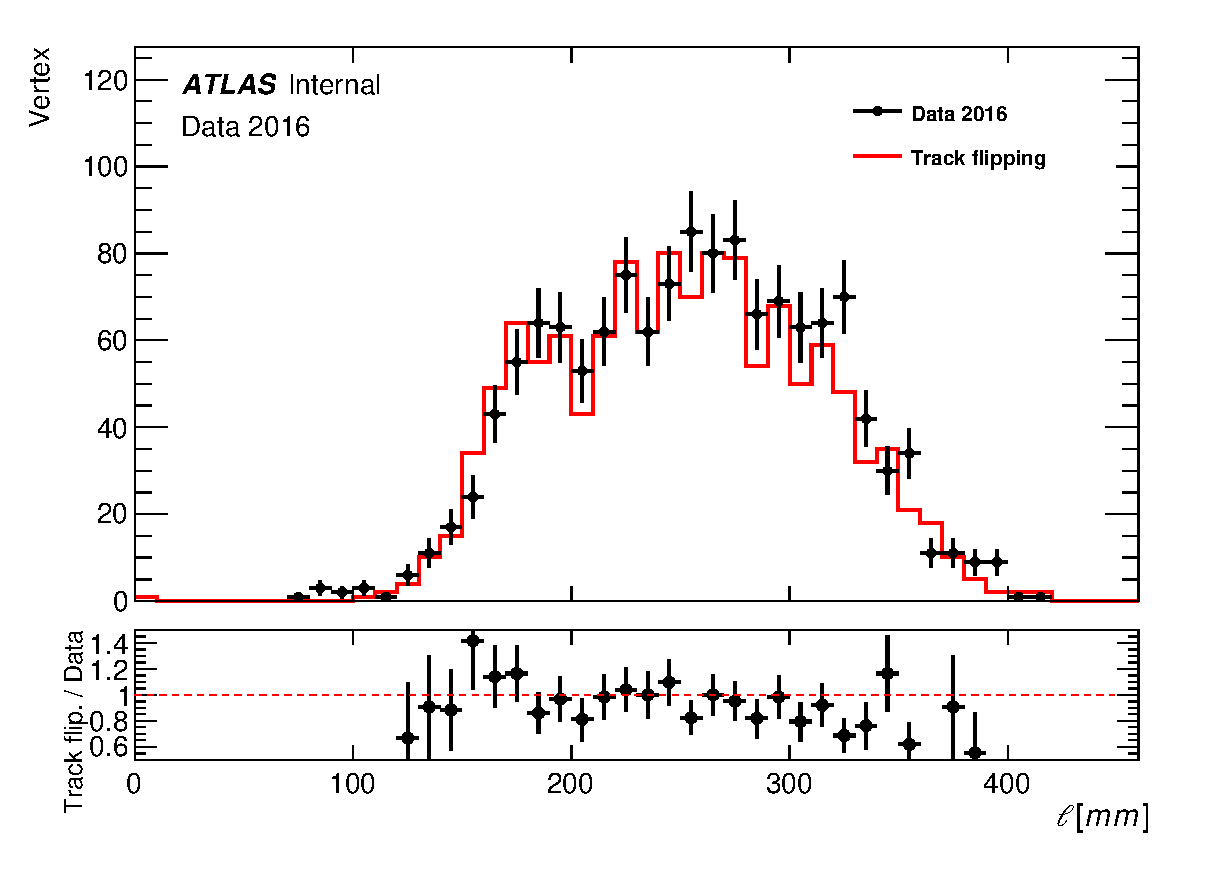
\includegraphics[width=0.45\textwidth]{figures/m_FBE_data_l.eps}}
    \caption{Comparison of (a) vertex mass, (b) $\chi^{2} / \mathrm{DOF}$, (c) transverse, and (d) longitudinal position of vertices found in data with vertices formed in track flipping in the control region. In (c), the red dashed lines indicate the four Pixel layers. The green dotted lines indicate the Inner Support Tube (45.5 mm) and Pixel Support Tube (229 mm).}
    \label{fig:random-crossing_vertex_dist_data}
\end{figure}

Because of the limited number of lepton pairs in the data sample, it is not practical to use the TF method to estimate the random-crossing background. Instead, the track-flipped vertex yields in the control region and validation region (region with zero or one lepton) are used to estimate random-crossing background in the signal region using the lepton probability, defined as follows:
\begin{itemize}
\item $P(e)$ is defined as the ratio of number of electrons to number of inner detector tracks in the entire sample,
\item $P(\mu)$ is defined as the ratio of number muons to number of inner detector tracks in the entire sample,
\end{itemize}
where track requirements described in Table~\ref{table:vertex_track_selection_simple} are imposed on both leptons and inner detector tracks. The lepton probability estimated from data is shown in Table~\ref{table:lepton_probability}.

\begin{table}[!htb]%
  \centering
    \begin{tabular}[t]{ccc}
        \hline\hline
                & Tracks             & P($\ell$)           \\
         \hline
         x      & $2.47\times10^{7}$ & -                   \\
         $\mu$  & $5.23\times10^{4}$ & $2.10\times10^{-3}$ \\
         $e$    & $3.63\times10^{4}$ & $1.46\times10^{-3}$ \\
         \hline
         Inclusive    & $2.48\times10^{7}$ & - \\
        \hline\hline
    \end{tabular}
  \caption{Number of x, $\mu$, $e$ tracks and the calculated lepton probability from data.}%
  \label{table:lepton_probability}
\end{table}


Using the lepton probabilities, the track-flipping vertex yield in the control region (xx) is extrapolated into the validation region using Eq.~\ref{eq:TF_extrapolation_from_validation}, and the extrapolated $\mu$x and $e$x vertex yields are compared with the observed track-flipping vertex yield to determine scale factors as defined in Eq~\ref{eq:random_crossing_scale_factor}.

The track-flipping vertex yields in the control and validation regions are then extrapolated into the signal region using Eqs.~\ref{eq:TF_extrapolation_from_control}$-$\ref{eq:TF_extrapolation_from_validation} to the estimate random-crossing background, and the scale factors (Eq.~\ref{eq:TF_scale_factors}) are applied to these extrapolation for a more precise estimate of the background.


The raw vertex yields in the TF method and data, and the scale factors calculated from the vertex yields are presented in Appendix~\ref{sec:tf_raw_yields}. The final estimate of random-crossing background from the TF method are shown in Table~\ref{table:track_flipping}. The estimate of the background after applying the scale factors in the signal region is $3.95\times10^{-3}$, which is compatible with the corresponding result of $2.40\times 10^{-3}$ from the event mixing method~\cite{DuarteCampderros:2275055}.


\begin{table}[!htb]%
  \centering
  \resizebox{\textwidth}{!}{
    \begin{tabular}[t]{cccc}
        \hline\hline
                                  & Raw estimate from xx & Raw estimate from $\mu$x, $e$x & Corrected estimate  \\
         \hline
         $N_{\mu\mu}$             & $2.69\times10^{-3}$  & $2.19\times10^{-3}$            & $1.79\times10^{-3}$ \\
         $N_{ee}$                 & $5.56\times10^{-3}$  & $1.05\times10^{-3}$            & $1.99\times10^{-4}$ \\
         $N_{e\mu}$               & $7.73\times10^{-3}$  & $3.89\times10^{-3}$            & $1.96\times10^{-3}$ \\
         \hline
         Sum of signal regions    & $1.60\times10^{-2}$  & $7.13\times10^{-3}$            & $3.95\times10^{-3}$ \\
        \hline\hline
    \end{tabular}
  }
  \caption{The estimate of random-crossing background in the signal region. Scale factors (Table~\ref{table:tf_raw_yields}) are applied to obtain the corrected estimate of the background.}%
  \label{table:track_flipping}
\end{table}





\chapter{Systematic Uncertainties}
\label{chap:syst}

\section{Systematics in Vertexing and Tracking}
\label{sec:syst:vertexing}


\chapter{Interpretation of Results}
\label{chap:upper_limit}

No events were observed in data that satisfies the signal selection, and the result is consistent with the SM expectations. Therefore, upper limits (ULs) are set on the cross section times branching ratio ($\sigma \times$ BR) for resonances decaying to a dilepton.

\section{Statistical Procedure}
The limits are calculated using \textit{HistFitter v0.61.0}~\cite{Baak:2014wma}, a statistical tool used for limit settings in ATLAS. The limit setting procedure is based on the modified Frequentist method, \CLs~\cite{OBRAZTSOV1992388,PhysRevD.57.3873}. In this framework, a number of events, $n$, is modeled as a Poisson distribution with the mean $\lambda = \mu_{\mathrm{sig}}\cdot s + b$ where $\mu_{\mathrm{sig}}$ is the signal strength parameter. The systematic uncertainty estimated in Chapter~\ref{chap:syst} is introduced as the nuisance parameter $\theta$ to $s$ and $b$, i.e. $s$ and $b$ become a function of $\theta$. The method uses the LHC default one-sided profile likelihood ratio $q_{\mu_{\mathrm{sig}}}$ as a test statistic,

\begin{equation}
q_{\mu_{\mathrm{sig}}} = -2 \log \Bigg( \dfrac{L(n_\mathrm{obs}~|~\mu_{n_\mathrm{sig}}, \Hat{\Hat{\theta}})}{L(n_\mathrm{obs}~|~\Hat{\mu}_{\mathrm{sig}}, \Hat{\theta})}\Bigg)
\label{eq:test_statistic}
\end{equation}
%
where $L$ is the likelihood function, $\Hat{\mu}_{\mathrm{sig}}$, $\Hat{\theta}$ are the values that globally maximize the likelihood, $\Hat{\Hat{\theta}}$ is the value that maximizes the likelihood for the specific value of $\mu_{\mathrm{sig}}$, and $n_{\mathrm{obs}}$ is the observed number of events in data or in pseudo experiments.

The distributions of the test statistic $q_{\mu_{\mathrm{sig}}}$ for the signal + background and background hypothesis ($\mu_{\mathrm{sig}} = 1$ or $\mu_{\mathrm{sig}} = 0$) are obtained from multiple pseudo experiments, and the Frequentist probability (or $p$-value) is calculated from the distributions as,

\begin{align}
\mathrm{CL}_{s+b} = P(q_{\mu_{\mathrm{sig}}} > q_{\mu_{\mathrm{sig}}}^{\mathrm{obs}}~|~\mu_{\mathrm{sig}} = 1), \nonumber \\
\mathrm{CL}_{b} = P(q_{\mu_{\mathrm{sig}}} > q_{\mu_{\mathrm{sig}}}^{\mathrm{obs}}~|~\mu_{\mathrm{sig}} = 0),
\label{eq:p_values}
\end{align}
%
where $\mathrm{CL}_{s+b}$ is the probability to obtain a test statistic value more extreme than the observed test statistic, $q_{\mu_{\mathrm{sig}}}^{\mathrm{obs}}$, assuming signal + background hypothesis ($\mu_{\mathrm{sig}}=1$), and $\mathrm{CL}_{b}$ is the corresponding probability for background hypothesis. Using these confidence levels, the signal confidence level, \CLs, is defined as
\begin{align}
\CLs =  \dfrac{\mathrm{CL}_{s+b}}{\mathrm{CL}_{b}}.
\label{eq:cls}
\end{align}

The UL at the 95\% confidence level are obtained by adjusting $\mu_{\mathrm{sig}}$ until \CLs reaches 0.05, and the limit is translated to the $\sigma \times$ BR by the relation,

\begin{equation}
\label{eq:signal_strength}
\mathcal{L}_{Int.} \cdot \big(\sigma \cdot \mathrm{BR} \big) \cdot \epsilon = \mu_{\mathrm{sig}}\cdot s + b,
\end{equation}
%
where $\mathcal{L}_{Int.}$ is the integrated luminosity and  $\epsilon$ is the signal efficiency.

\section{Upper limits}
The observed ULs are evaluated by performing pseudo experiments with an expected background of 0.27$\pm$0.14 events, the systematic uncertainty of 10\%, and the uncertainty of the luminosity measurement of 2.2\%.

The observed ULs at 95\% CL on $\sigma \times$ BR for $Z' \rightarrow$ \mumu, \ee, and \emu are shown in Figure~\ref{fig:upper_limits} as a function of $c\tau$. The observed limits are relatively uniform in $c\tau$ for all channels. At $m_{Z'}=$ 1 TeV, the ULs are from 0.5 - 0.9 fb. At $m_{Z'}=$ 100 GeV, the ULs are much larger (50 - 400 pb) than other mass points due to the limited trigger efficiency.


\begin{figure}[!htb]
    \centering
    \subfloat[]{\label{subfig:ul_mumu}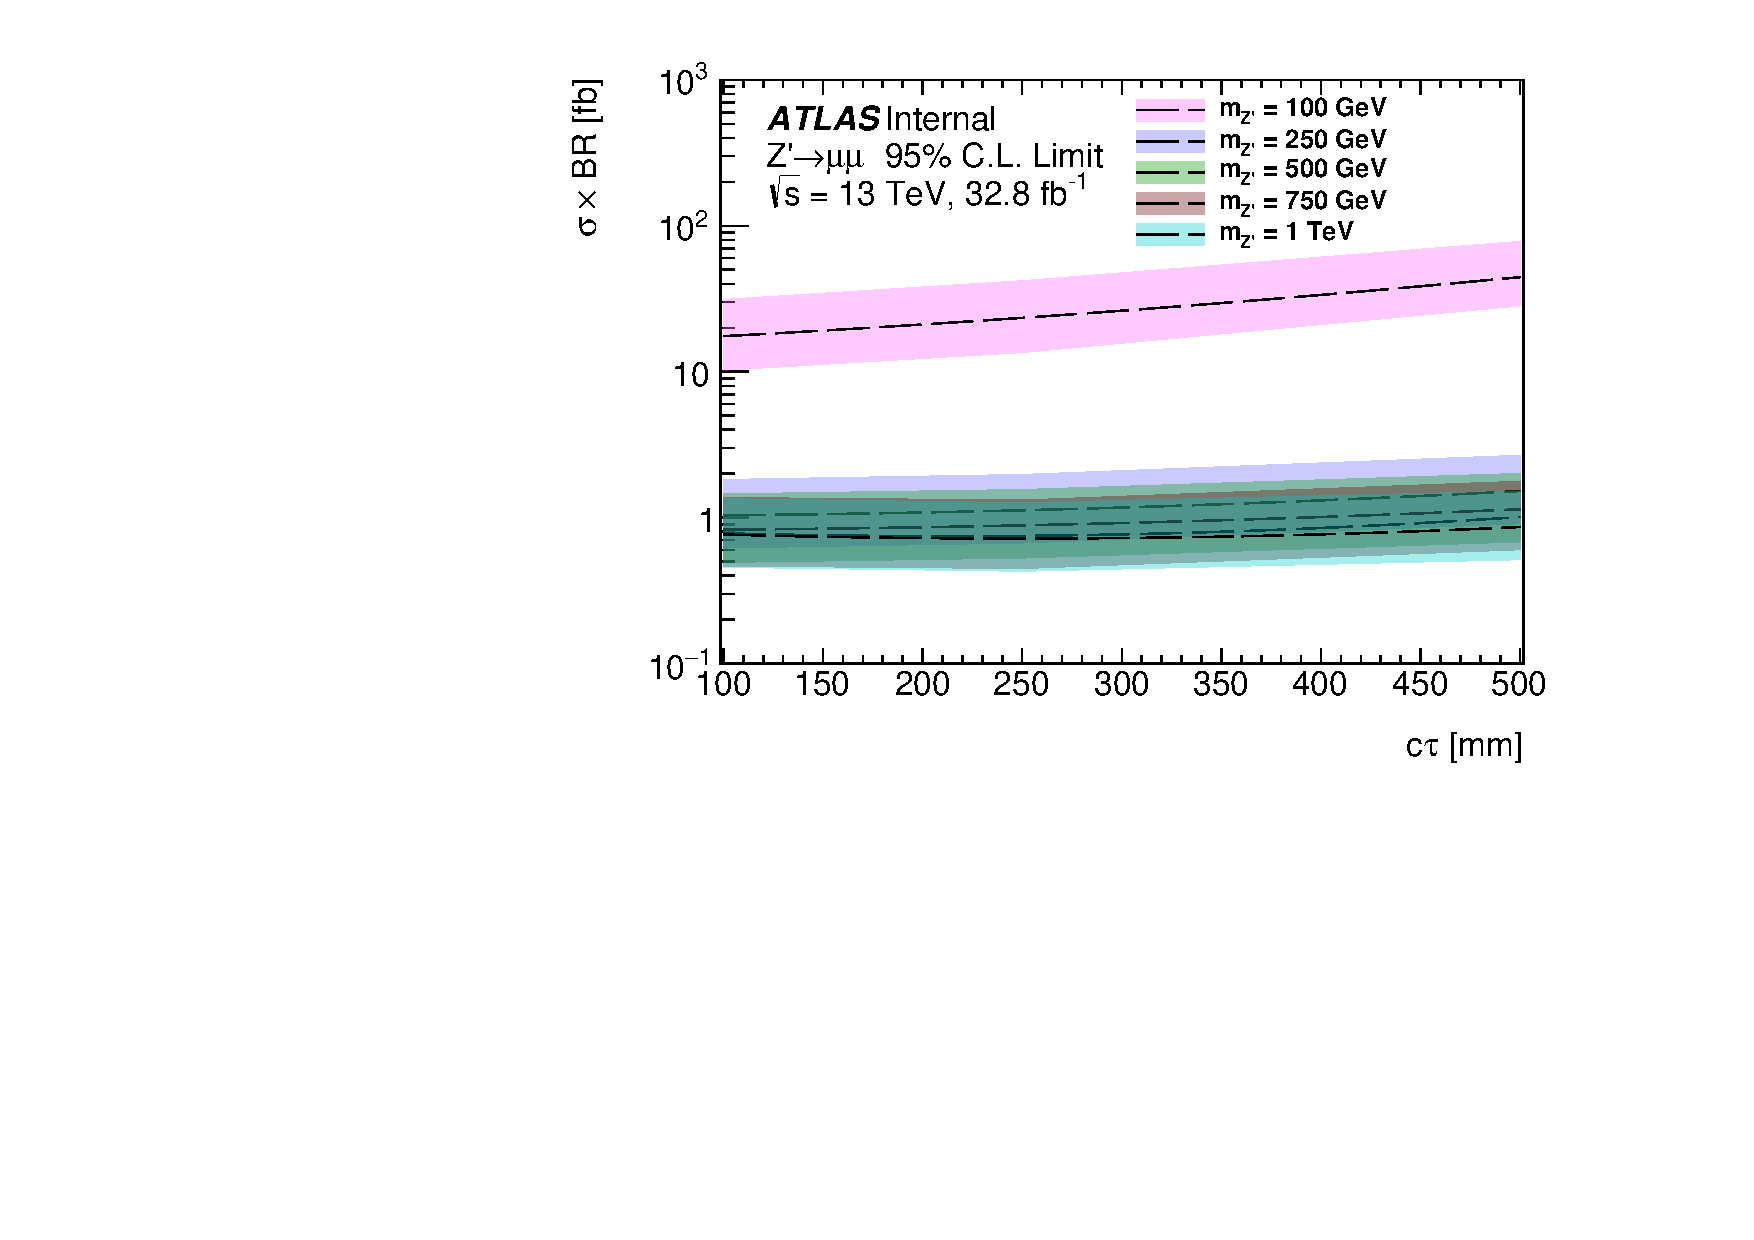
\includegraphics[width=0.60\textwidth]{figures/UL/DiMu_UL.pdf}} \\
    \subfloat[]{\label{subfig:ul_ee}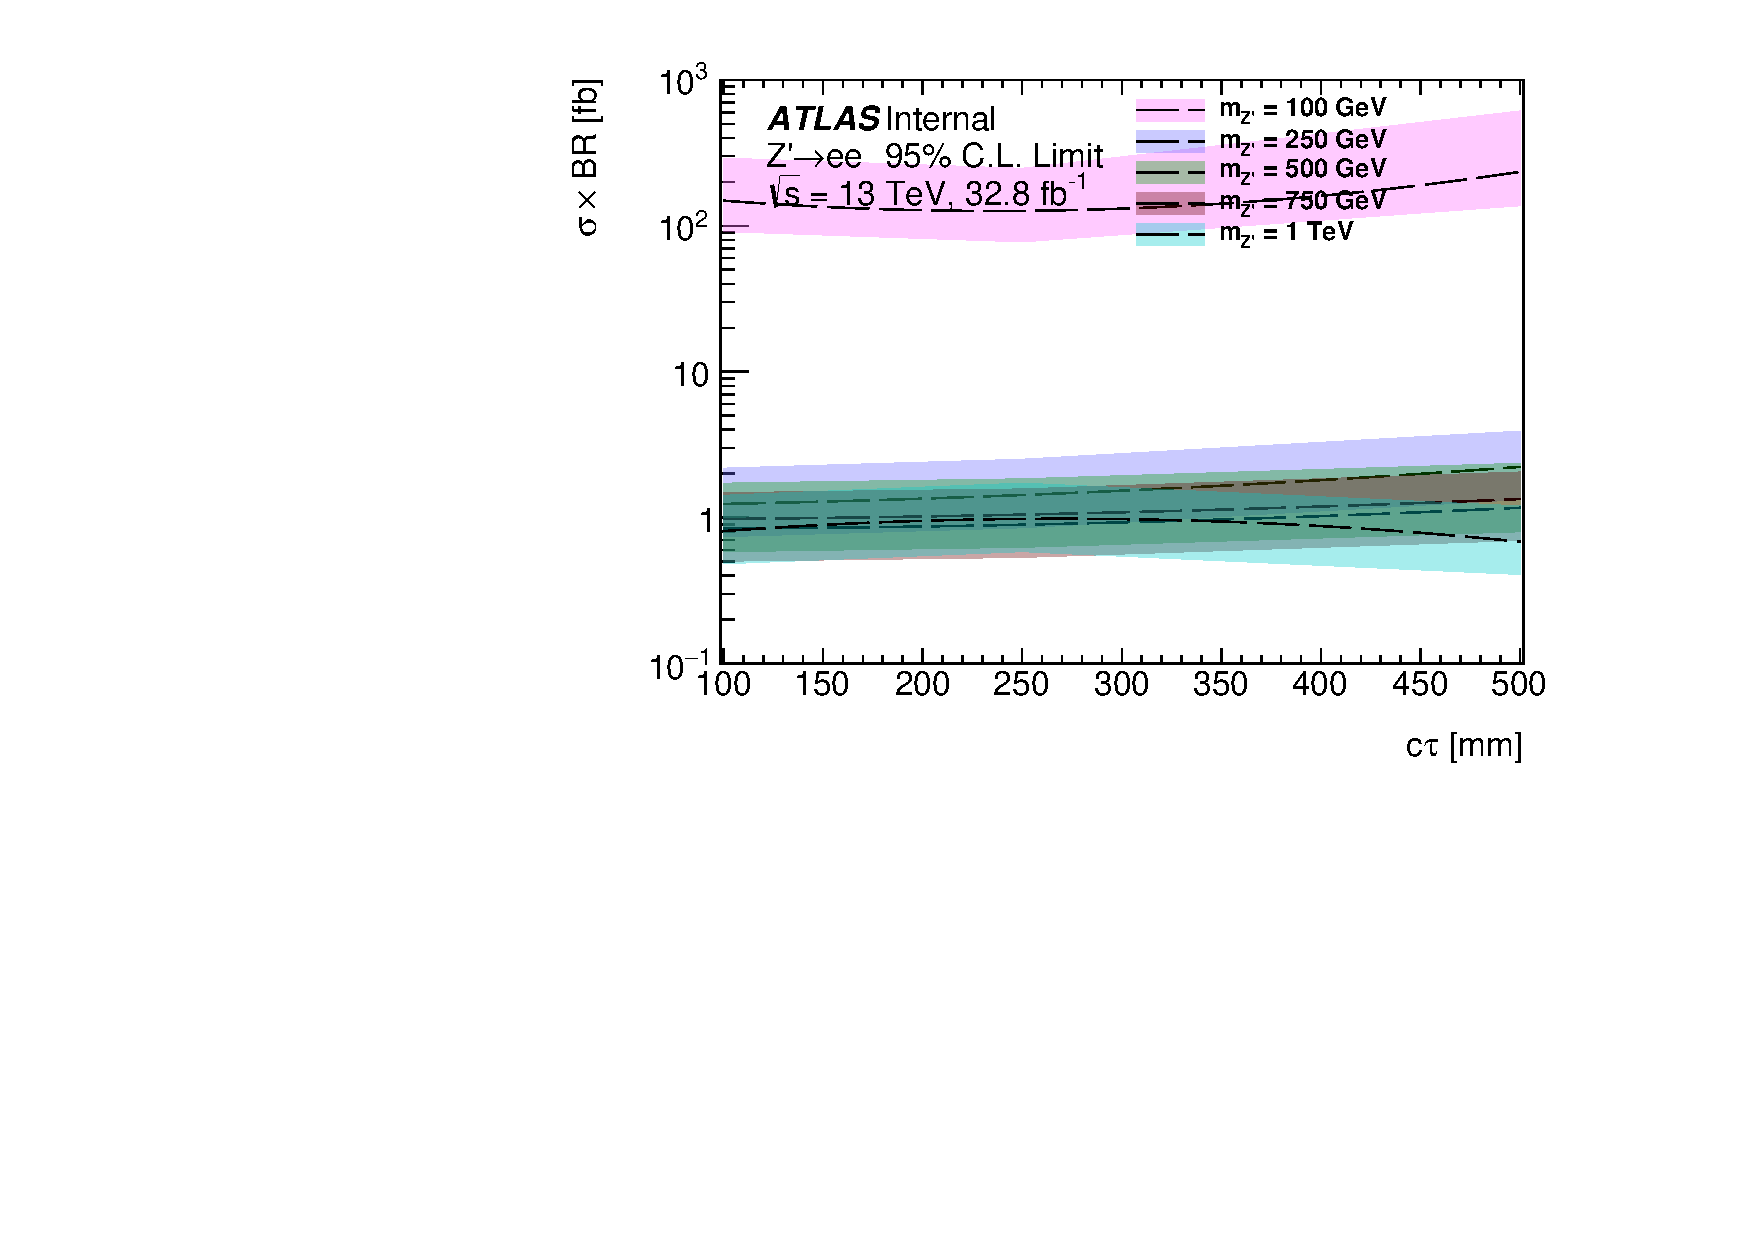
\includegraphics[width=0.60\textwidth]{figures/UL/DiE_UL.pdf}}    \\
    \subfloat[]{\label{subfig:ul_emu}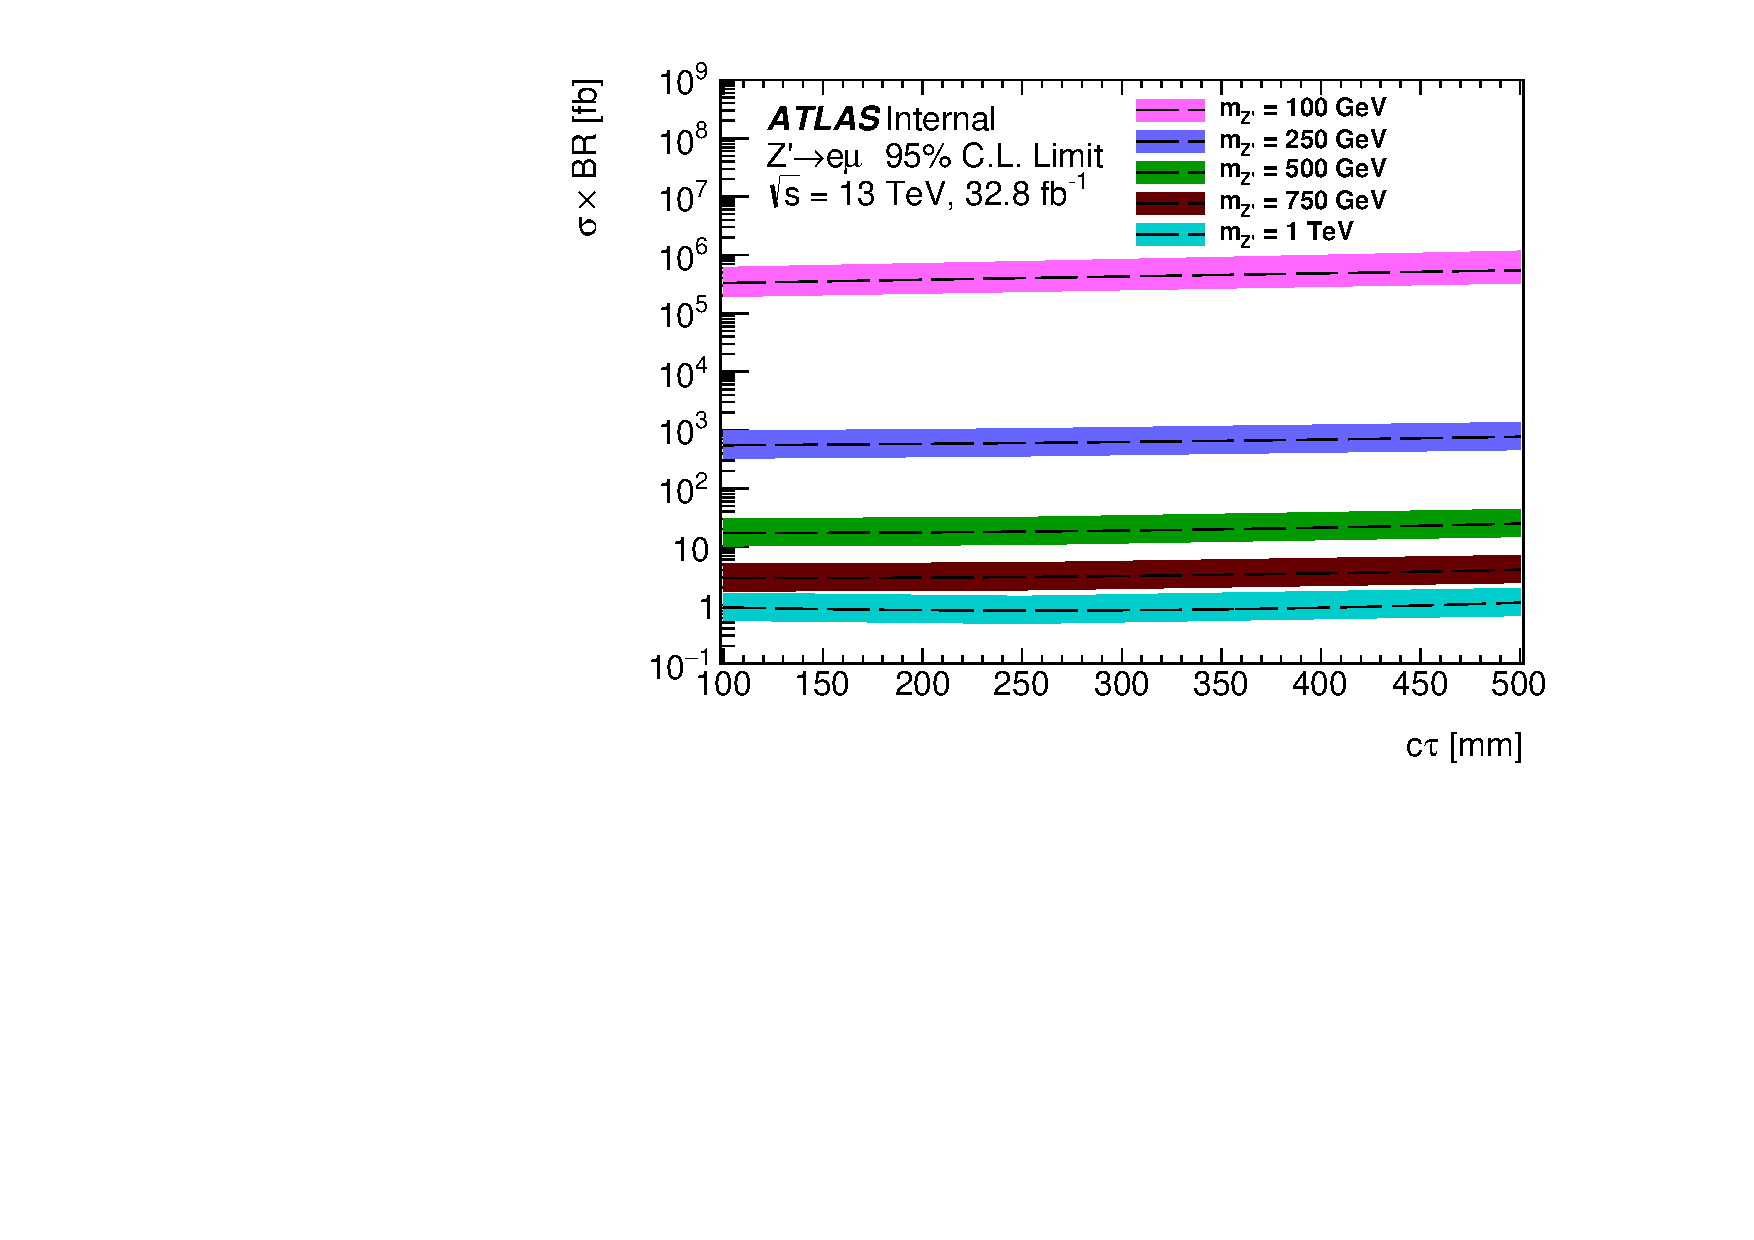
\includegraphics[width=0.60\textwidth]{figures/UL/EMu_UL.pdf}}   \\
    \caption{The observed 95$\%$ CL upper limits on the $\sigma \times$ BR for the $Z'\rightarrow$ (a) \mumu, (b) \ee, and (c) \emu signal samples with $Z'$ masses of 100 - 1000 GeV as a function of $c\tau$. The dashed lines are expected limits, and the solid bands represent 1$\sigma$ uncertainty on the expected limit.}
    \label{fig:upper_limits}
\end{figure}


\chapter{Conclusion}
\label{chap:conclusion}

A search for long-lived $Z'$ decaying to a $\mu\mu$, $ee$, or $e\mu$ pair is performed using 32.8 $\mathrm{fb^{-1}}$ of $pp$ collisions at $\sqrt{s}=13$ TeV with the ATLAS detector at the LHC. No event was observed, and the results are consistent with an expected background of 0.27$\pm$0.14 events. Upper limits are set on $\sigma \times$ BR for resonances decaying to a dilepton, and the resulting upper limits at the 95\% CL are between 50 - 400 pb at $m_{Z'}=$ 100 GeV and 0.5 - 0.9 fb at $m_{Z'}=$ 1 TeV. %These upper limits exclude significant regions of the parameter space in search for long-lived particles.
Also presented is the signal efficiency as a function of $p_{T}$ and $\eta$ for resonances decaying to a dilepton with typical values range from 10 - 20\% within the tracking coverage.



%\nocite{*} % To display all refs, even uncited refs (useful when editting)
%\bibliography
\cleardoublepage
\phantomsection
\addcontentsline{toc}{chapter}{Bibliography}
\bibliography{thesis}
%\bibliographystyle{h-physrev}
\bibliographystyle{atlasBibStyleWithTitle}
%\bibliographystyle{ieeetr}
%\bibliographystyle{unsrt} % use your favorite BIBTeX style



%\appendix
\begin{appendices}
\addcontentsline{toc}{chapter}{Appendices}
\renewcommand{\thesection}{\Alph{section}}
\titleformat{\section}{\centering\Large\bfseries}{\appendixname~\thesection:}{0.5em}{}
%\renewcommand{\thetable}{A\arabic{table}}
\renewcommand\thetable{\Alph{section}.\arabic{table}}
\renewcommand\thefigure{\Alph{section}.\arabic{figure}}
\renewcommand\theequation{\Alph{section}.\arabic{equation}}

\clearpage
\section{Trigger efficiency}
\label{app:trig_eff}
The trigger efficiency of all $Z'$ signal MC samples is shown in Table~\ref{table:m_trig_eff_mumu}. It is evident that at low $Z'$ mass ($\sim$100 GeV), the combined trigger efficiency of the signal MC sample is significantly reduced because the typical $p_{T}$ of the signal leptons is lower than the $p_{T}$ threshold of the trigger.



\begin{table}[!htb]
  \centering
  \resizebox{\textwidth}{!}{
  \begin{tabular}{ c c | c c c c}
    \hline
    \hline
    $m_{Z'}$ (GeV) & $c\tau$ (mm) & Single muon (\%) & Single photon (\%) & Di-photon (\%) & Combined (\%) \\
    \hline
	100             &100    &4.70$\pm$0.15  &0.01$\pm$0.01  &0.00$\pm$0.00  &4.70$\pm$0.15 \\
	100             &250    &4.09$\pm$0.14  &0.00$\pm$0.00  &0.00$\pm$0.00  &4.09$\pm$0.14 \\
	100             &500    &3.81$\pm$0.14  &0.00$\pm$0.00  &0.00$\pm$0.00  &3.81$\pm$0.14 \\
	250             &100    &34.57$\pm$0.34 &0.08$\pm$0.02  &0.04$\pm$0.01  &34.65$\pm$0.34 \\
	250             &250    &30.84$\pm$0.33 &0.07$\pm$0.02  &0.03$\pm$0.01  &30.90$\pm$0.33 \\
	250             &500    &24.41$\pm$0.30 &0.05$\pm$0.02  &0.01$\pm$0.01  &24.45$\pm$0.30 \\
	500             &100    &47.60$\pm$0.36 &1.02$\pm$0.07  &0.10$\pm$0.02  &48.14$\pm$0.36 \\
	500             &250    &40.82$\pm$0.35 &1.00$\pm$0.07  &0.13$\pm$0.03  &41.36$\pm$0.35 \\
	500             &500    &33.15$\pm$0.33 &0.80$\pm$0.06  &0.10$\pm$0.02  &33.62$\pm$0.33 \\
	750             &100    &53.99$\pm$0.35 &2.68$\pm$0.11  &0.28$\pm$0.04  &55.16$\pm$0.35 \\
	750             &250    &46.99$\pm$0.35 &2.27$\pm$0.11  &0.26$\pm$0.04  &48.11$\pm$0.35 \\
	750             &500    &39.18$\pm$0.35 &2.23$\pm$0.10  &0.13$\pm$0.03  &40.30$\pm$0.35 \\
	1000            &100    &56.91$\pm$0.35 &3.96$\pm$0.14  &0.35$\pm$0.04  &58.46$\pm$0.35 \\
	1000            &250    &51.13$\pm$0.35 &3.59$\pm$0.13  &0.33$\pm$0.04  &52.58$\pm$0.35 \\
	1000            &500    &43.14$\pm$0.35 &3.24$\pm$0.13  &0.34$\pm$0.04  &44.52$\pm$0.35 \\
    \hline
    \hline
  \end{tabular}
  }
  \caption{Trigger efficiency of single muon, single photon, di-photon triggers, and the combined trigger efficiency of the signal MC samples of $Z'\rightarrow\mumu$. Statistical uncertainty is shown.}
  \label{table:m_trig_eff_mumu}
\end{table}

\begin{table}[!htb]
  \centering
  \subfloat[]{
  \resizebox{\textwidth}{!}{
  \begin{tabular}{ c c | c c c c}
    \hline
    \hline
    $m_{Z'}$ (GeV) & $c\tau$ (mm) & Single muon (\%) & Single photon (\%) & Di-photon (\%) & Combined (\%) \\
    \hline
	100             &100    &0.00$\pm$0.00  &0.30$\pm$0.04  &1.36$\pm$0.08  &1.57$\pm$0.09 \\
	100             &250    &0.00$\pm$0.00  &0.31$\pm$0.04  &1.37$\pm$0.08  &1.62$\pm$0.09 \\
	100             &500    &0.02$\pm$0.01  &0.37$\pm$0.04  &0.97$\pm$0.07  &1.21$\pm$0.08 \\
	250             &100    &0.00$\pm$0.00  &8.12$\pm$0.19  &49.26$\pm$0.35 &50.73$\pm$0.35 \\
	250             &250    &0.00$\pm$0.00  &6.74$\pm$0.18  &45.00$\pm$0.35 &46.38$\pm$0.35 \\
	250             &500    &0.01$\pm$0.01  &5.80$\pm$0.17  &37.21$\pm$0.34 &38.78$\pm$0.34 \\
	500             &100    &0.02$\pm$0.01  &73.59$\pm$0.31 &66.73$\pm$0.33 &80.06$\pm$0.28 \\
	500             &250    &0.02$\pm$0.01  &68.10$\pm$0.33 &60.90$\pm$0.35 &74.28$\pm$0.31 \\
	500             &500    &0.02$\pm$0.01  &59.35$\pm$0.36 &51.22$\pm$0.36 &64.62$\pm$0.35 \\
	750             &100    &0.02$\pm$0.01  &87.99$\pm$0.23 &74.83$\pm$0.31 &90.07$\pm$0.21 \\
	750             &250    &0.03$\pm$0.01  &82.54$\pm$0.27 &68.60$\pm$0.33 &84.60$\pm$0.26 \\
	750             &500    &0.02$\pm$0.01  &74.59$\pm$0.31 &58.39$\pm$0.35 &76.45$\pm$0.30 \\
	1000            &100    &0.03$\pm$0.01  &92.45$\pm$0.19 &79.87$\pm$0.28 &93.61$\pm$0.17 \\
	1000            &250    &0.01$\pm$0.01  &88.44$\pm$0.23 &73.84$\pm$0.31 &89.45$\pm$0.22 \\
	1000            &500    &0.04$\pm$0.01  &81.57$\pm$0.28 &64.60$\pm$0.35 &82.45$\pm$0.28 \\
    \hline
    \hline
  \end{tabular}
  }
  }
  \caption{Trigger efficiency of single muon, single photon, di-photon triggers, and the combined trigger efficiency of the signal MC samples of $Z'\rightarrow \ee$. Statistical uncertainty is shown.}
  \label{table:m_trig_eff_ee}
\end{table}



\begin{table}[!htb]
  \centering
  \subfloat[]{
  \resizebox{\textwidth}{!}{
  \begin{tabular}{ c c | c c c c}
    \hline
    \hline
    $m_{Z'}$ (GeV) & $c\tau$ (mm) & Single muon (\%) & Single photon (\%) & Di-photon (\%) & Combined (\%) \\
    \hline
	100             &100    &2.35$\pm$0.11  &0.16$\pm$0.03  &0.05$\pm$0.02  &2.55$\pm$0.11 \\
	100             &250    &2.24$\pm$0.10  &0.15$\pm$0.03  &0.07$\pm$0.02  &2.41$\pm$0.11 \\
	100             &500    &1.79$\pm$0.10  &0.17$\pm$0.03  &0.06$\pm$0.02  &2.00$\pm$0.10 \\
	250             &100    &20.22$\pm$0.28 &4.09$\pm$0.14  &1.12$\pm$0.07  &23.85$\pm$0.30 \\
	250             &250    &18.28$\pm$0.27 &3.58$\pm$0.13  &0.92$\pm$0.07  &21.36$\pm$0.29 \\
	250             &500    &14.87$\pm$0.25 &3.02$\pm$0.12  &0.54$\pm$0.05  &17.43$\pm$0.27 \\
	500             &100    &27.30$\pm$0.32 &62.39$\pm$0.35 &3.31$\pm$0.13  &70.26$\pm$0.33 \\
	500             &250    &24.01$\pm$0.30 &57.40$\pm$0.35 &2.88$\pm$0.12  &63.40$\pm$0.34 \\
	500             &500    &20.66$\pm$0.29 &49.46$\pm$0.35 &2.27$\pm$0.11  &54.43$\pm$0.35 \\
	750             &100    &31.74$\pm$0.34 &78.47$\pm$0.30 &4.88$\pm$0.16  &83.85$\pm$0.27 \\
	750             &250    &28.27$\pm$0.32 &73.66$\pm$0.31 &4.68$\pm$0.15  &77.73$\pm$0.29 \\
	750             &500    &23.33$\pm$0.30 &64.74$\pm$0.34 &3.99$\pm$0.14  &67.99$\pm$0.33 \\
	1000            &100    &34.07$\pm$0.35 &84.66$\pm$0.27 &6.35$\pm$0.18  &88.72$\pm$0.24 \\
	1000            &250    &30.27$\pm$0.32 &79.67$\pm$0.28 &5.85$\pm$0.17  &83.16$\pm$0.26 \\
	1000            &500    &26.61$\pm$0.32 &71.87$\pm$0.33 &5.21$\pm$0.16  &74.55$\pm$0.32 \\
    \hline
    \hline
  \end{tabular}
  }
  }
  \caption{Trigger efficiency of single muon, single photon, di-photon triggers, and the combined trigger efficiency of the signal MC samples of $Z'\rightarrow \emu$. Statistical uncertainty is shown.}
  \label{table:m_trig_eff_emu}
\end{table}







\clearpage
\begin{sidewaysfigure}[!htb]
\section{Efficiency Map of Signal MC Samples}
\label{app:signal_efficiency_map}
    \centering
    \subfloat[$m=100$ GeV, $c\tau=100$ mm]{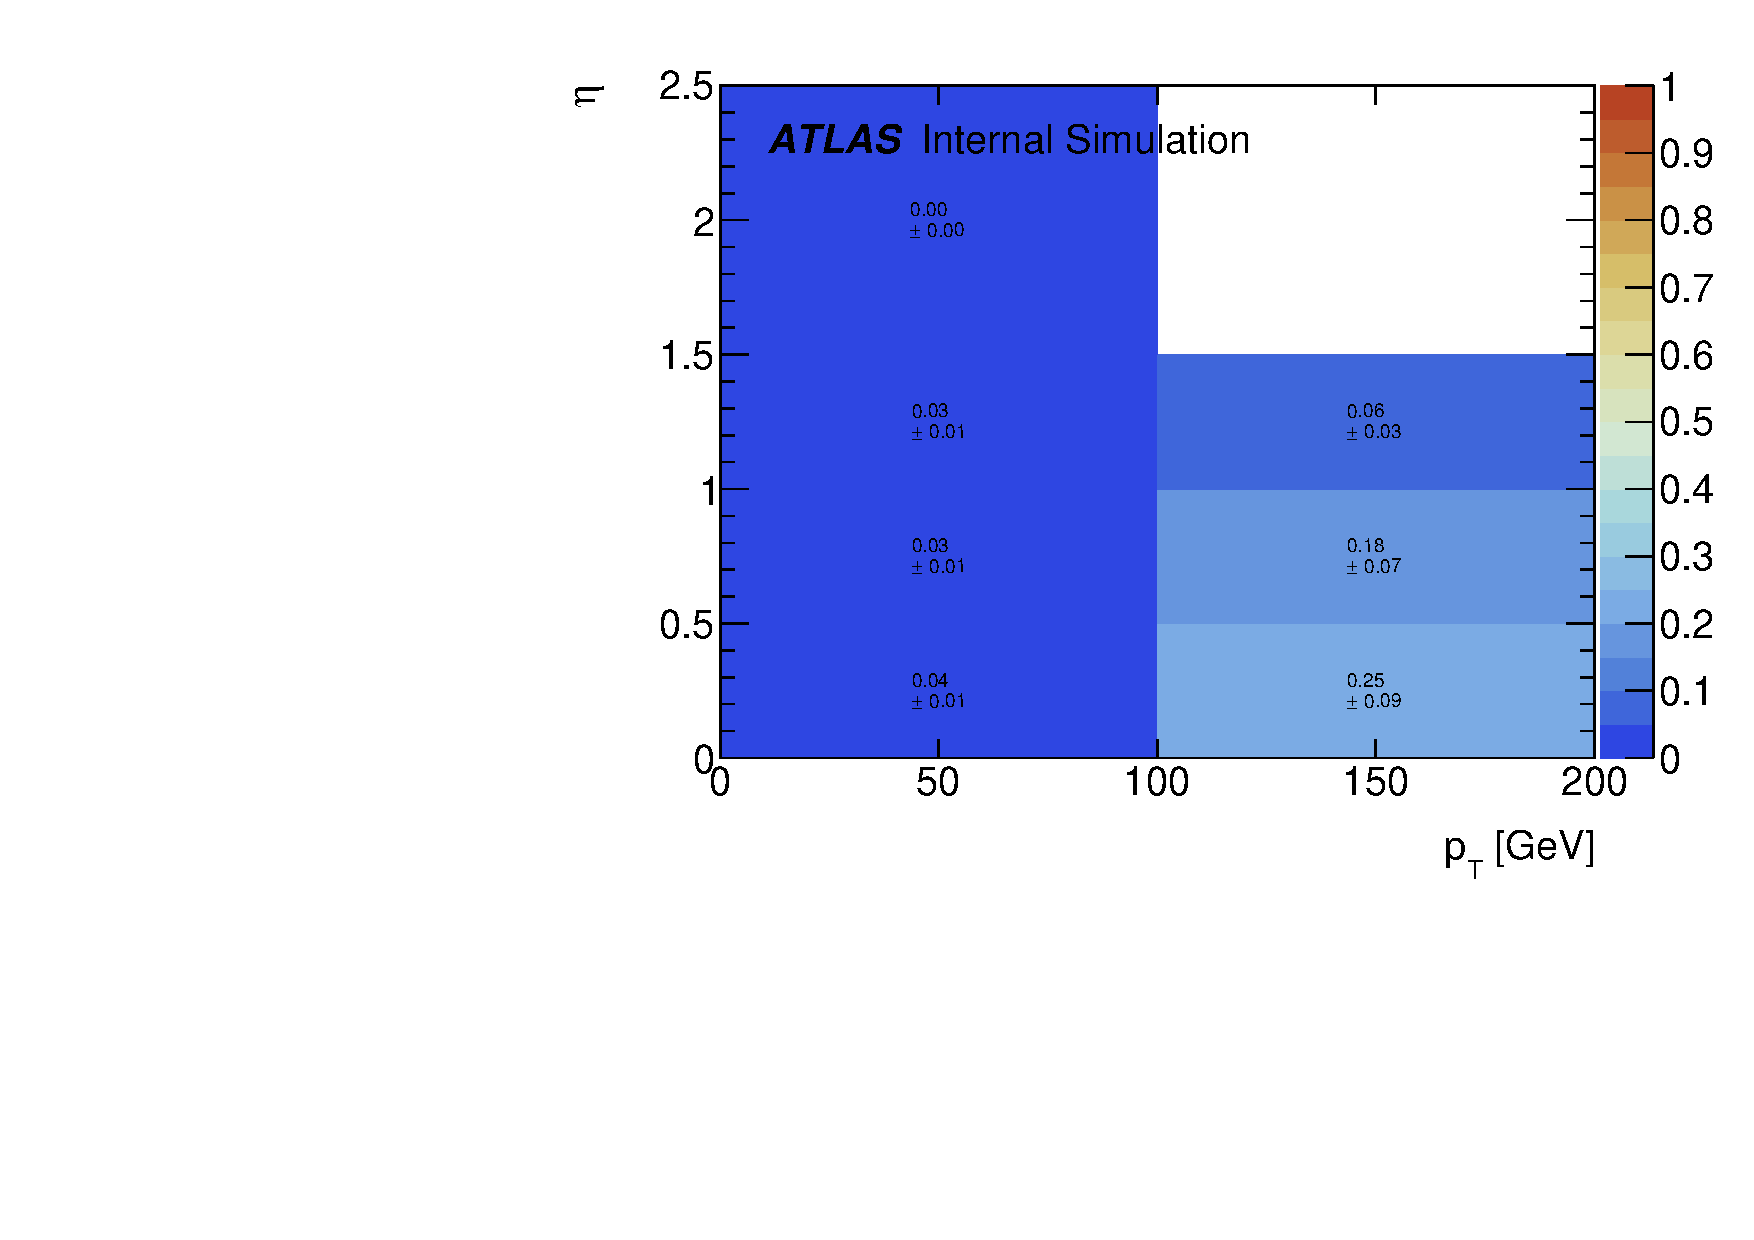
\includegraphics[width=0.33\textwidth]{figures/EfficiencyMap/eff_map_mumu_m100t100.pdf}}
    \subfloat[$m=100$ GeV, $c\tau=250$ mm]{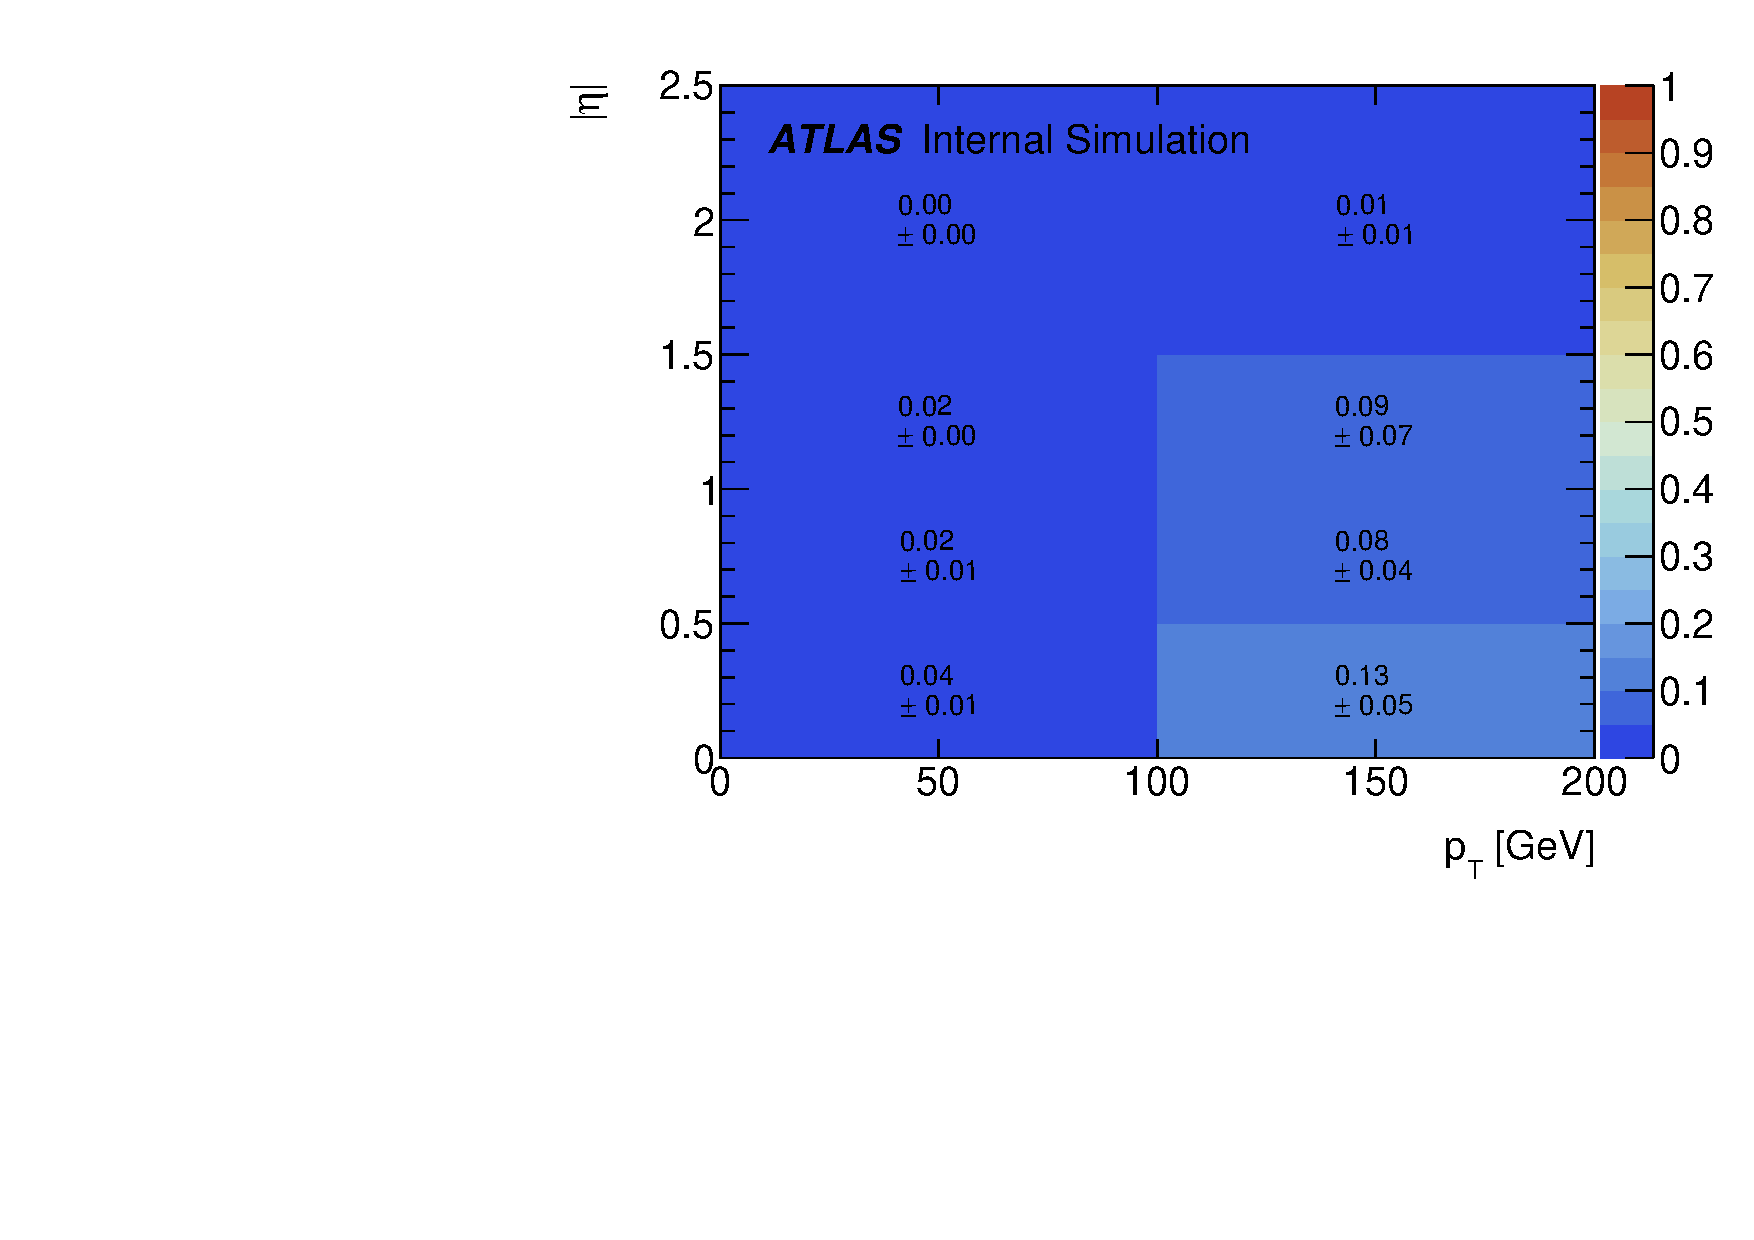
\includegraphics[width=0.33\textwidth]{figures/EfficiencyMap/eff_map_mumu_m100t250.pdf}}
    \subfloat[$m=100$ GeV, $c\tau=500$ mm]{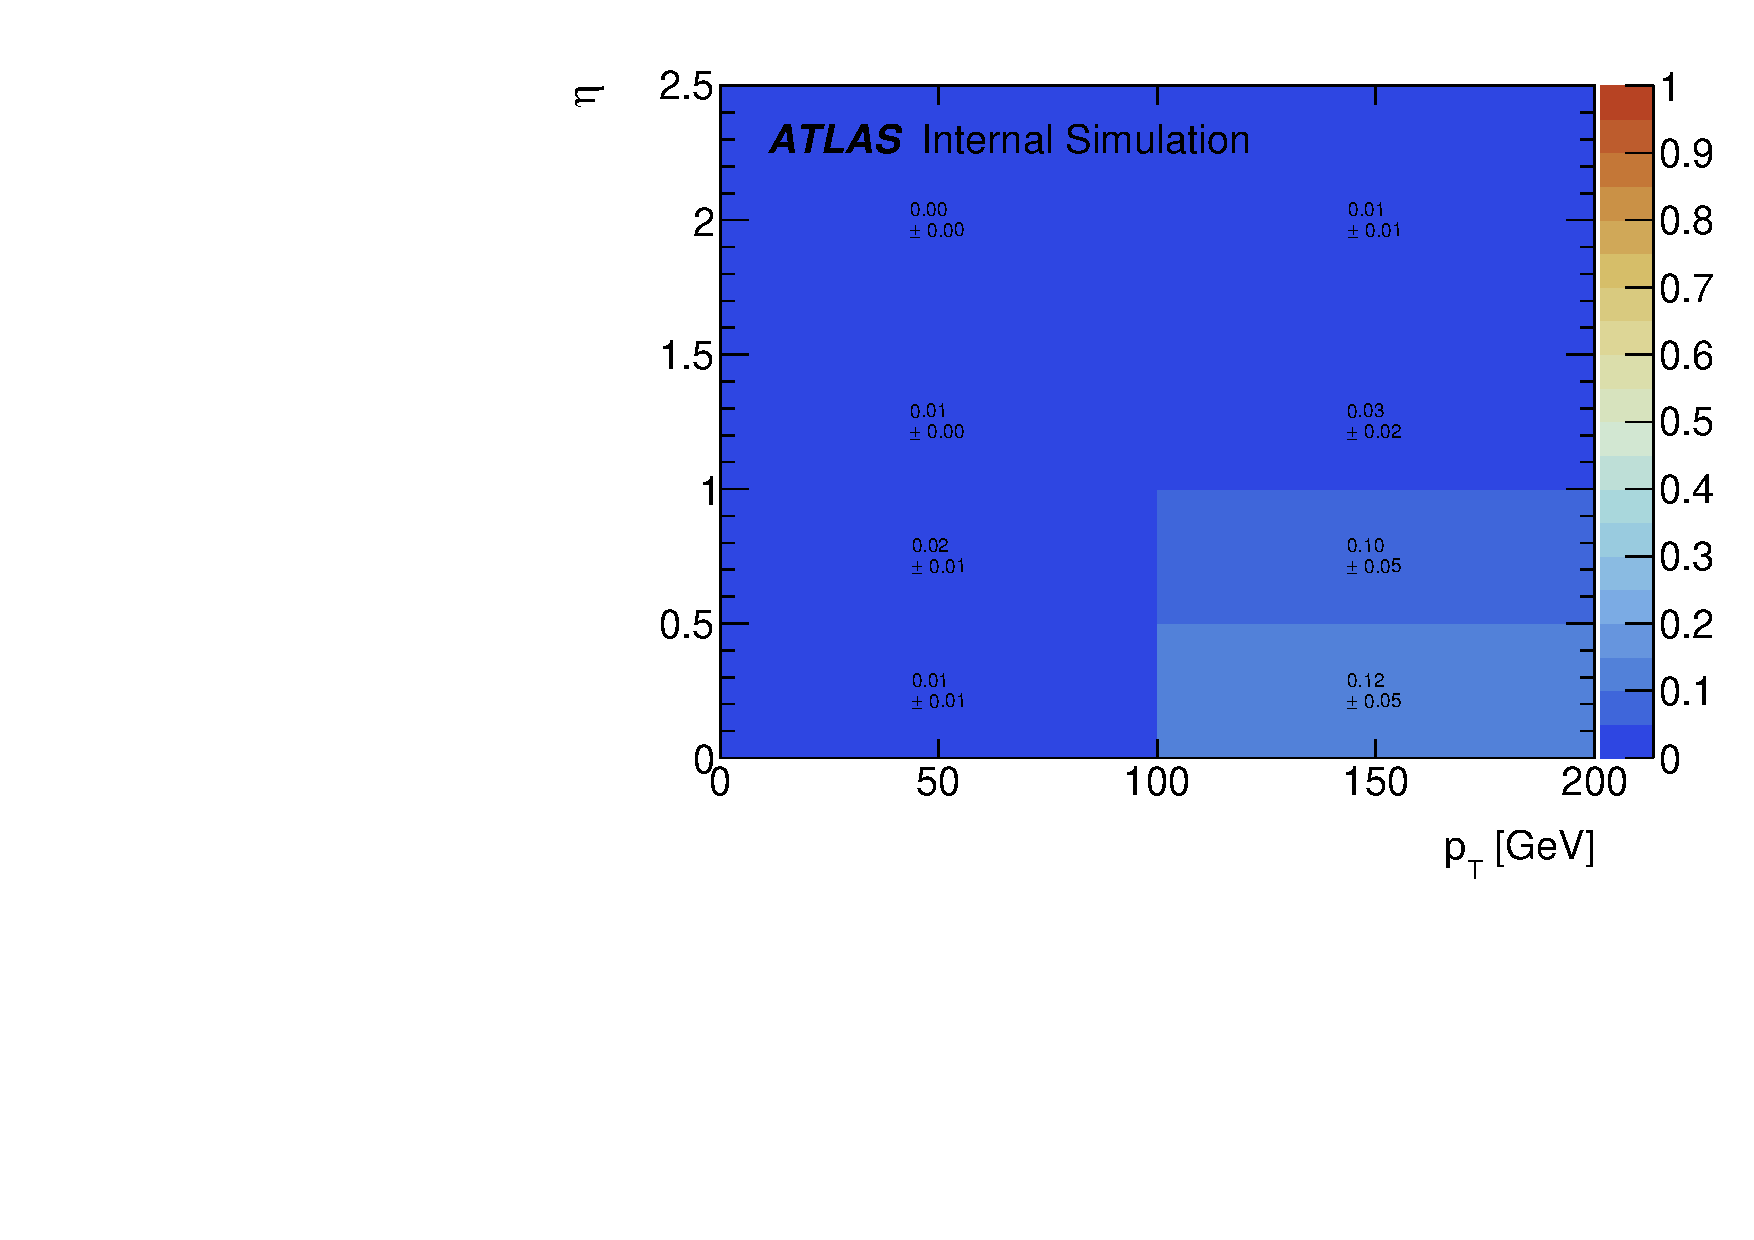
\includegraphics[width=0.33\textwidth]{figures/EfficiencyMap/eff_map_mumu_m100t500.pdf}}\\
    \subfloat[$m=250$ GeV, $c\tau=100$ mm]{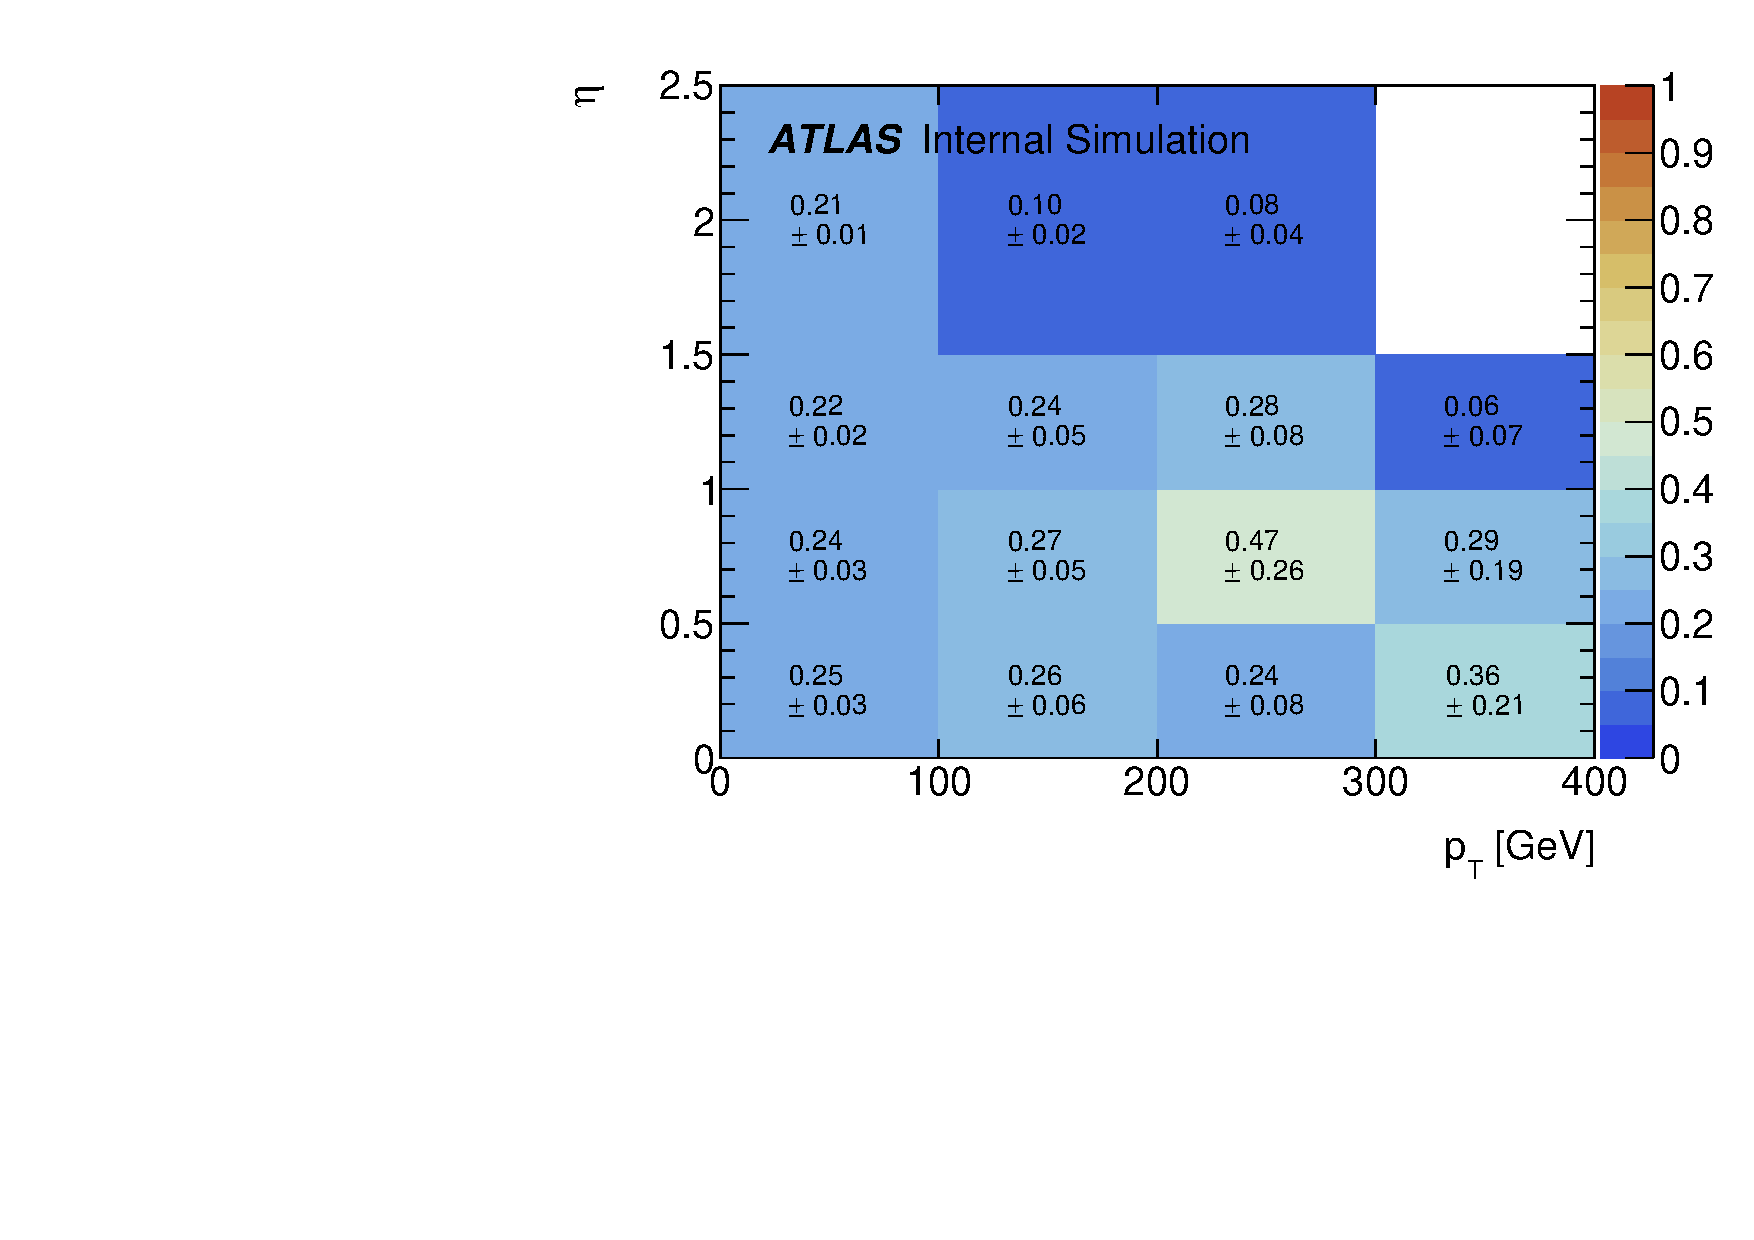
\includegraphics[width=0.33\textwidth]{figures/EfficiencyMap/eff_map_mumu_m250t100.pdf}}
    \subfloat[$m=250$ GeV, $c\tau=250$ mm]{\includegraphics[width=0.33\textwidth]{figures/EfficiencyMap/eff_map_mumu_m250t250.pdf}}
    \subfloat[$m=250$ GeV, $c\tau=500$ mm]{\includegraphics[width=0.33\textwidth]{figures/EfficiencyMap/eff_map_mumu_m250t500.pdf}}\\
\caption{Reconstruction efficiency map of $|\eta|$ vs. $p_{T}$ for $Z' \rightarrow \mumu$ MC sample with $m_{Z'} = $ 100 and 250 GeV.}
\label{fig:signal_eff_map_app1}
\end{sidewaysfigure}

\begin{sidewaysfigure}[!htb]
    \centering
    \subfloat[$m=500$ GeV, $c\tau=100$ mm]{\includegraphics[width=0.30\textwidth]{figures/EfficiencyMap/eff_map_mumu_m500t100.pdf}}
    \subfloat[$m=500$ GeV, $c\tau=250$ mm]{\includegraphics[width=0.30\textwidth]{figures/EfficiencyMap/eff_map_mumu_m500t250.pdf}}
    \subfloat[$m=500$ GeV, $c\tau=500$ mm]{\includegraphics[width=0.30\textwidth]{figures/EfficiencyMap/eff_map_mumu_m500t500.pdf}}\\
    \subfloat[$m=750$ GeV, $c\tau=100$ mm]{\includegraphics[width=0.30\textwidth]{figures/EfficiencyMap/eff_map_mumu_m750t100.pdf}}
    \subfloat[$m=750$ GeV, $c\tau=250$ mm]{\includegraphics[width=0.30\textwidth]{figures/EfficiencyMap/eff_map_mumu_m750t250.pdf}}
    \subfloat[$m=750$ GeV, $c\tau=500$ mm]{\includegraphics[width=0.30\textwidth]{figures/EfficiencyMap/eff_map_mumu_m750t500.pdf}}\\
    \subfloat[$m=1000$ GeV, $c\tau=100$ mm]{\includegraphics[width=0.30\textwidth]{figures/EfficiencyMap/eff_map_mumu_m1000t100.pdf}}
    \subfloat[$m=1000$ GeV, $c\tau=250$ mm]{\includegraphics[width=0.30\textwidth]{figures/EfficiencyMap/eff_map_mumu_m1000t250.pdf}}
    \subfloat[$m=1000$ GeV, $c\tau=500$ mm]{\includegraphics[width=0.30\textwidth]{figures/EfficiencyMap/eff_map_mumu_m1000t500.pdf}} 
\caption{Reconstruction efficiency map of $|\eta|$ vs. $p_{T}$ for $Z' \rightarrow \mumu$ MC sample with $m_{Z'} = $ 500, 750 and 1000 GeV.}
\label{fig:signal_eff_map_app2}
\end{sidewaysfigure}

\begin{sidewaysfigure}[!htb]
    \centering
    \subfloat[$m=100$ GeV, $c\tau=100$ mm]{\includegraphics[width=0.30\textwidth]{figures/EfficiencyMap/eff_map_ee_m100t100.pdf}}
    \subfloat[$m=100$ GeV, $c\tau=250$ mm]{\includegraphics[width=0.30\textwidth]{figures/EfficiencyMap/eff_map_ee_m100t250.pdf}}
    \subfloat[$m=100$ GeV, $c\tau=500$ mm]{\includegraphics[width=0.30\textwidth]{figures/EfficiencyMap/eff_map_ee_m100t500.pdf}}\\
    \subfloat[$m=250$ GeV, $c\tau=100$ mm]{\includegraphics[width=0.30\textwidth]{figures/EfficiencyMap/eff_map_ee_m250t100.pdf}}
    \subfloat[$m=250$ GeV, $c\tau=250$ mm]{\includegraphics[width=0.30\textwidth]{figures/EfficiencyMap/eff_map_ee_m250t250.pdf}}
    \subfloat[$m=250$ GeV, $c\tau=500$ mm]{\includegraphics[width=0.30\textwidth]{figures/EfficiencyMap/eff_map_ee_m250t500.pdf}}\\
    \subfloat[$m=500$ GeV, $c\tau=100$ mm]{\includegraphics[width=0.30\textwidth]{figures/EfficiencyMap/eff_map_ee_m500t100.pdf}}
    \subfloat[$m=500$ GeV, $c\tau=250$ mm]{\includegraphics[width=0.30\textwidth]{figures/EfficiencyMap/eff_map_ee_m500t250.pdf}}
    \subfloat[$m=500$ GeV, $c\tau=500$ mm]{\includegraphics[width=0.30\textwidth]{figures/EfficiencyMap/eff_map_ee_m500t500.pdf}}
\caption{Reconstruction efficiency map of $|\eta|$ vs. $p_{T}$ for $Z' \rightarrow \ee$ MC sample with $m_{Z'} = $ 100, 250 and 500 GeV.}
\label{fig:signal_eff_map_app3}
\end{sidewaysfigure}


\begin{sidewaysfigure}[!htb]
    \centering
    \subfloat[$m=750$ GeV, $c\tau=100$ mm]{\includegraphics[width=0.33\textwidth]{figures/EfficiencyMap/eff_map_ee_m750t100.pdf}}
    \subfloat[$m=750$ GeV, $c\tau=250$ mm]{\includegraphics[width=0.33\textwidth]{figures/EfficiencyMap/eff_map_ee_m750t250.pdf}}
    \subfloat[$m=750$ GeV, $c\tau=500$ mm]{\includegraphics[width=0.33\textwidth]{figures/EfficiencyMap/eff_map_ee_m750t500.pdf}}\\
    \subfloat[$m=1000$ GeV, $c\tau=100$ mm]{\includegraphics[width=0.33\textwidth]{figures/EfficiencyMap/eff_map_ee_m1000t100.pdf}}
    \subfloat[$m=1000$ GeV, $c\tau=250$ mm]{\includegraphics[width=0.33\textwidth]{figures/EfficiencyMap/eff_map_ee_m1000t250.pdf}}
    \subfloat[$m=1000$ GeV, $c\tau=500$ mm]{\includegraphics[width=0.33\textwidth]{figures/EfficiencyMap/eff_map_ee_m1000t500.pdf}} 
\caption{Reconstruction efficiency map of $|\eta|$ vs. $p_{T}$ for $Z' \rightarrow \ee$ MC sample with $m_{Z'} = $ 750 and 1000 GeV.}
\label{fig:signal_eff_map_app4}
\end{sidewaysfigure}

\begin{sidewaysfigure}[!htb]
    \centering
    \subfloat[$m=100$ GeV, $c\tau=100$ mm]{\includegraphics[width=0.30\textwidth]{figures/EfficiencyMap/eff_map_emu_m100t100.pdf}}
    \subfloat[$m=100$ GeV, $c\tau=250$ mm]{\includegraphics[width=0.30\textwidth]{figures/EfficiencyMap/eff_map_emu_m100t250.pdf}}
    \subfloat[$m=100$ GeV, $c\tau=500$ mm]{\includegraphics[width=0.30\textwidth]{figures/EfficiencyMap/eff_map_emu_m100t500.pdf}}\\
    \subfloat[$m=250$ GeV, $c\tau=100$ mm]{\includegraphics[width=0.30\textwidth]{figures/EfficiencyMap/eff_map_emu_m250t100.pdf}}
    \subfloat[$m=250$ GeV, $c\tau=250$ mm]{\includegraphics[width=0.30\textwidth]{figures/EfficiencyMap/eff_map_emu_m250t250.pdf}}
    \subfloat[$m=250$ GeV, $c\tau=500$ mm]{\includegraphics[width=0.30\textwidth]{figures/EfficiencyMap/eff_map_emu_m250t500.pdf}}\\
    \subfloat[$m=500$ GeV, $c\tau=100$ mm]{\includegraphics[width=0.30\textwidth]{figures/EfficiencyMap/eff_map_emu_m500t100.pdf}}
    \subfloat[$m=500$ GeV, $c\tau=250$ mm]{\includegraphics[width=0.30\textwidth]{figures/EfficiencyMap/eff_map_emu_m500t250.pdf}}
    \subfloat[$m=500$ GeV, $c\tau=500$ mm]{\includegraphics[width=0.30\textwidth]{figures/EfficiencyMap/eff_map_emu_m500t500.pdf}}
\caption{Reconstruction efficiency map of $|\eta|$ vs. $p_{T}$ for $Z' \rightarrow \emu$ MC sample with $m_{Z'} = $ 100, 250 and 500 GeV.}
\label{fig:signal_eff_map_app5}
\end{sidewaysfigure}


\begin{sidewaysfigure}[!htb]
    \centering
    \subfloat[$m=750$ GeV, $c\tau=100$ mm]{\includegraphics[width=0.33\textwidth]{figures/EfficiencyMap/eff_map_emu_m750t100.pdf}}
    \subfloat[$m=750$ GeV, $c\tau=250$ mm]{\includegraphics[width=0.33\textwidth]{figures/EfficiencyMap/eff_map_emu_m750t250.pdf}}
    \subfloat[$m=750$ GeV, $c\tau=500$ mm]{\includegraphics[width=0.33\textwidth]{figures/EfficiencyMap/eff_map_emu_m750t500.pdf}}\\
    \subfloat[$m=1000$ GeV, $c\tau=100$ mm]{\includegraphics[width=0.33\textwidth]{figures/EfficiencyMap/eff_map_emu_m1000t100.pdf}}
    \subfloat[$m=1000$ GeV, $c\tau=250$ mm]{\includegraphics[width=0.33\textwidth]{figures/EfficiencyMap/eff_map_emu_m1000t250.pdf}}
    \subfloat[$m=1000$ GeV, $c\tau=500$ mm]{\includegraphics[width=0.33\textwidth]{figures/EfficiencyMap/eff_map_emu_m1000t500.pdf}} 
\caption{Reconstruction efficiency map of $|\eta|$ vs. $p_{T}$ for $Z' \rightarrow \emu$ MC sample with $m_{Z'} = $ 750 and 1000 GeV.}
\label{fig:signal_eff_map_app6}
\end{sidewaysfigure}



\clearpage
\section{\texorpdfstring{$K_{S}$}{Ks} and \texorpdfstring{$Z'$}{Z'} comparison}
\label{app:syst_Ks_Zp}

The ideal $K_{S}$ sample to estimate the systematic uncertainty in track and vertex reconstruction should have the same kinematic distributions as the $Z'$ MC sample. Obviously, the two samples have different distributions. Figure~\ref{fig:Ks_zp_comparison} shows comparisons of the vertex/kenematic distributions. The reconstructed $K_{S}$ and $Z'$ vertices are required to match to a $K_{S}$ and $Z'$ vertex produced at truth level with spatial displacement no larger than $0.7$ mm. All distributions are normalized to unity. It is fortuitous that their distribution cover the $r$ region of interest, and the two samples have similar $z$ distribution.


\begin{figure}[!htb]
    \centering
    \subfloat[]{\label{subfig:Ks_zp_r}\includegraphics[width=0.40\textwidth]{figures/m_syst_zp_Ks_r.pdf}}
    \subfloat[]{\label{subfig:Ks_zp_z}\includegraphics[width=0.40\textwidth]{figures/m_syst_zp_Ks_z.pdf}} \\
    \subfloat[]{\label{subfig:Ks_zp_eta}\includegraphics[width=0.40\textwidth]{figures/m_syst_zp_Ks_eta.pdf}} 
    \subfloat[]{\label{subfig:Ks_zp_pt}\includegraphics[width=0.40\textwidth]{figures/m_syst_zp_Ks_pt.pdf}} \\
    %\subfloat[]{\label{subfig:Ks_zp_z}\includegraphics[width=0.40\textwidth]{figures/m_syst_zp_Ks_DeltaR.pdf}}
    \caption{Distribution of transverse (a), longitudinal vertex position (b), $\eta$ (c), $p_{T}$ (d), and the opening angle between decay particles of $K_{S}$ and $Z'$ vertices (e) found in the background and the signal MC sample described in Section~\ref{sec:background_mc_sample}. Distributions are normalized to unity. Systematic uncertainties are shown.}
    \label{fig:Ks_zp_comparison}
\end{figure}



\clearpage
\section{Extrapolation in the track flipping method}
In this section, the extrapolation method used in the TF method is derived. The TF method yields vertices in the control (\xx), validation (\mux, \ex), and signal region (\mumu, \ee, \emu) which represent the estimate of random-crossing background in each region. However, because of limited number in lepton pairs in the data sample, it is not practical to use the vertex yields in the signal region to estimate the background. Instead, the vertex yields in the control and validation region are extrapolated into the signal region in order to estimate the random-crossing background.



\subsection{Definition}
In this derivation, the following definition of $\mu$, $e$, and x is used where lepton and non-leptonic tracks are mutually exclusive.
\begin{itemize}
\item x = tracks that are not $\mu$ or $e$
\item $e$ = electron tracks
\item $\mu$ = muon tracks 
\end{itemize}

Furthermore, the following conventions for the number of tracks, pairs, vertices, and lepton probability are used.
\begin{itemize}
\item $N^{\mathrm{T}}_{\mathrm{x}}$, $N^{\mathrm{T}}_{e}$, $N^{\mathrm{T}}_{\mu}$ represent number of x, $e$, and $\mu$ tracks, respectively.
\item $N^{\mathrm{R}}_{\mathrm{xx}}$, $N^{\mathrm{R}}_{\mu \mathrm{x}}$, $N^{\mathrm{R}}_{e\mathrm{x}}$, $N^{\mathrm{R}}_{\mu\mu}$, $N^{\mathrm{R}}_{ee}$, $N^{\mathrm{R}}_{e\mu}$ represent the number of pairs of each type.
\item $N_{\mathrm{xx}}$, $N_{\mu \mathrm{x}}$, $N_{e\mathrm{x}}$, $N_{\mu\mu}$, $N_{ee}$, $N_{e\mu}$ represent the number of vertices of each type.
\item $P(\mu) = \frac{N^{\mathrm{T}}_{\mu}}{N^{\mathrm{T}}_{\mu} + N^{\mathrm{T}}_{e} + N^{\mathrm{T}}_{\mathrm{x}}}$ represent the muon probability.
\item $P(e) = \frac{N^{\mathrm{T}}_{e}}{N^{\mathrm{T}}_{\mu} + N^{\mathrm{T}}_{e} + N^{\mathrm{T}}_{\mathrm{x}}}$ represent the electron probability.
\end{itemize}


\subsection{Vertex estimation}
A number of reconstructed vertices in the sample can be estimated by the number of track pairs in the sample and the probability of a pair to form a vertex, i.e.

\begin{equation}
N_{\mathrm{xx}} = N^{\mathrm{R}}_{\mathrm{xx}} \times P(\mathrm{xx}),
\end{equation}
%
where $P(\mathrm{xx})$ is the probability for a $xx$ pair to form a vertex. Similarly, the vertexing probability for track pairs in the validation and signal region can be defined as below.

\begin{align}
\label{estimation_generic}
N_{\mu \mathrm{x}}& = N^{\mathrm{R}}_{\mu \mathrm{x}} \times P(\mu \mathrm{x}), \nonumber \\
N_{e\mathrm{x}} &= N^{\mathrm{R}}_{e\mathrm{x}} \times P(e\mathrm{x}), \nonumber \\
N_{\mu\mu} &= N^{\mathrm{R}}_{\mu\mu} \times P(\mu\mu), \nonumber \\
N_{ee} &= N^{\mathrm{R}}_{ee} \times P(ee), \nonumber \\
N_{e \mu} &= N^{\mathrm{R}}_{e \mu} \times P(e\mu).
\end{align}



\subsection{Counting pairs}
Given a collection of x tracks in a single event, the number of all possible pairs can be expressed as,
\begin{equation}
\label{counting_pairs1}
N^{\mathrm{R}}_{\mathrm{xx}} = \binom{N^{\mathrm{T}}_{\mathrm{x}}}{2} = \frac{N^{\mathrm{T}}_{\mathrm{x}}!}{(N^{\mathrm{T}}_{\mathrm{x}}-2)!\cdot 2!} = \frac{1}{2} \cdot (N^{\mathrm{T}}_{\mathrm{x}}\cdot(N^{\mathrm{T}}_{\mathrm{x}}-1)).
\end{equation}
%
Given two different sets of tracks, for example x and $\mu$, the number of possible pairs is
\begin{equation}
N^{\mathrm{R}}_{\mu \mathrm{x}} = N^{\mathrm{T}}_{\mu} \cdot N^{\mathrm{T}}_{\mathrm{x}}.
\end{equation}
%
Similarly, the number of pairs from other combinations of tracks are
\begin{align}
\label{counting_pairs2}
N^{\mathrm{R}}_{ee} &= \binom{N^{\mathrm{T}}_{e}}{2} = \frac{N^{\mathrm{T}}_{e}!}{(N^{\mathrm{T}}_{e}-2)!\cdot 2!} = \frac{1}{2} \cdot (N^{\mathrm{T}}_{e}\cdot(N^{\mathrm{T}}_{e}-1)), \nonumber\\
N^{\mathrm{R}}_{\mu\mu} &= \binom{N^{\mathrm{T}}_{\mu}}{2} = \frac{N^{\mathrm{T}}_{\mu}!}{(N^{\mathrm{T}}_{\mu}-2)!\cdot 2!} = \frac{1}{2} \cdot (N^{\mathrm{T}}_{\mu}\cdot(N^{\mathrm{T}}_{\mu}-1)), \nonumber\\
N^{\mathrm{R}}_{e\mathrm{x}} &= N^{\mathrm{T}}_{e} \cdot N^{\mathrm{T}}_{\mathrm{x}},\nonumber \\
N^{\mathrm{R}}_{e \mu} &= N^{\mathrm{T}}_{e} \cdot N^{\mathrm{T}}_{\mu}.
\end{align}

Note that Eq.~\ref{counting_pairs1}-\ref{counting_pairs2} are only true event-wise. If there are $N^{\mathrm{T}}_{\mathrm{x}}$ tracks in data, it can not be directly translated to $N^{\mathrm{R}}_{\mathrm{xx}}$ using Eq.~\ref{counting_pairs1}. Instead, the sum of $N^{\mathrm{R}}_{\mathrm{xx}}$ from each event needs to be calculated.

%In the following discussion, I will naively think of data as one big event since all events should behave the same in large data. 
%However, this means that we cannot directly use quantities like $N^{\mathrm{T}}_{\mathrm{x}}$ and $N^{\mathrm{R}}_{\mathrm{xx}}$, and we are only allowed to use the probabilities and total vertex yields from data.


\subsection{Extrapolation of control region into validation and signal region}

The track-flipped vertex yield in the control region can be extrapolated into the validation and signal region as follows.

Given a number of tracks ($\mu$, $e$, x), we can estimate the number of vertices in the validation and signal region using Eq.~\ref{counting_pairs1}$-$Eq.~\ref{counting_pairs2} and Eq.~\ref{estimation_generic}. However, since the vertexing probabilities in the validation and signal region ($P(\mu \mathrm{x})$, $P(e\mathrm{x})$, etc..) are unknown without using the information from those regions, the vertexing probability obtained from the control region ($P(\mathrm{xx})$) can be used as an estimation of the vertexing probability in the validation and the signal region. $P(\mathrm{xx})$ can be expressed as,

\begin{align}
\label{p_xx}
P(\mathrm{xx}) &= \frac{N_{\mathrm{xx}}^{obs}}{N^{\mathrm{R}}_{\mathrm{xx}}} = \frac{N_{\mathrm{xx}}^{obs}}{{\frac{1}{2} \cdot (N^{\mathrm{T}}_{\mathrm{x}}\cdot(N^{\mathrm{T}}_{\mathrm{x}}-1))}}.
\end{align}
%
Using Eq.~\ref{estimation_generic} and Eq.~\ref{p_xx}, the vertex yield in the validation and signal region can be estimated as,

\begin{align}
\label{eq:TF_extrapolation_from_control}
N_{\mu \mathrm{x}}^{est} &= N^{\mathrm{R}}_{\mu \mathrm{x}} \cdot P(\mu \mathrm{x}) \approx N^{\mathrm{R}}_{\mu \mathrm{x}} \cdot P(\mathrm{xx})    = 2 \cdot \frac{N^{\mathrm{T}}_{\mu}}{N^{\mathrm{T}}_{\mathrm{x}} -1} \cdot N_{\mathrm{xx}}^{obs} \approx 2 \cdot P(\mu) \cdot N_{\mathrm{xx}}^{obs},\nonumber\\
N_{e \mathrm{x}}^{est}   &= N^{\mathrm{R}}_{e \mathrm{x}} \cdot P(e\mathrm{x}) \approx N^{\mathrm{R}}_{e \mathrm{x}} \cdot P(\mathrm{xx})      = 2 \cdot \frac{N^{\mathrm{T}}_{e}}{N^{\mathrm{T}}_{\mathrm{x}} -1} \cdot N_{\mathrm{xx}}^{obs} \approx 2 \cdot P(e) \cdot N_{\mathrm{xx}}^{obs}, \nonumber \\
N_{\mu\mu}^{est}&= N^{\mathrm{R}}_{\mu\mu} \times P(\mu\mu) \approx N^{\mathrm{R}}_{\mu\mu} \times P(\mathrm{xx})  = \frac{N^{\mathrm{T}}_{\mu}\cdot(N^{\mathrm{T}}_{\mu} - 1)}{N^{\mathrm{T}}_{\mathrm{x}}\cdot(N^{\mathrm{T}}_{\mathrm{x}}-1)} \cdot N_{\mathrm{xx}}^{obs} \approx P(\mu)^{2} \cdot N_{\mathrm{xx}}^{obs}, \nonumber \\
N_{ee}^{est}    &= N^{\mathrm{R}}_{ee} \times P(ee) \approx N^{\mathrm{R}}_{ee} \times P(\mathrm{xx}) 		= \frac{N^{\mathrm{T}}_{e}\cdot(N^{\mathrm{T}}_{e} - 1)}{N^{\mathrm{T}}_{\mathrm{x}}\cdot(N^{\mathrm{T}}_{\mathrm{x}}-1)} \cdot N_{\mathrm{xx}}^{obs} \approx P(e)^{2} \cdot N_{\mathrm{xx}}^{obs}, \nonumber \\
N_{e \mu}^{est} &= N^{\mathrm{R}}_{e \mu} \times P(e \mu) \approx N^{\mathrm{R}}_{e \mu} \times P(\mathrm{xx}) 	= N^{\mathrm{T}}_{e} \cdot N^{\mathrm{T}}_{\mu} \frac{2 \cdot N_{\mathrm{xx}}^{obs}}{N^{\mathrm{T}}_{\mathrm{x}} \cdot (N^{\mathrm{T}}_{\mathrm{x}}-1)} \approx 2\cdot P(e)\cdot P(\mu) \cdot N_{\mathrm{xx}}^{obs},
\end{align}
%
where $N^{obs}$ represents measured track-flipped vertex yield in the data and $N^{est}$ represents the estimated vertex yield in the validation and signal region by the extrapolation.

\subsection{Extrapolation of validation region into signal region}

Similarly, the track-flipped vertex yield in the validation region can be extrapolated into the signal region by $P(\mu\mathrm{x})$ and $P(\mathrm{x})$ as estimates of $P(\mu\mu)$ and $P(ee)$ where

\begin{align}
P(\mu\mathrm{x}) &= \frac{N_{\mu\mathrm{x}}^{obs}}{N^{\mathrm{R}}_{\mu\mathrm{x}}} = \frac{N_{\mu\mathrm{x}}^{obs}}{N^{\mathrm{T}}_{\mu} \cdot N^{\mathrm{T}}_{\mathrm{x}}}, \nonumber\\
P(\mathrm{x}) &= \frac{N_{ex}^{obs}}{N^{\mathrm{R}}_{ex}} = \frac{N_{ex}^{obs}}{N^{\mathrm{T}}_{e} \cdot N^{\mathrm{T}}_{\mathrm{x}}}.
\end{align}
%
Using $P(\mu\mathrm{x})$ and $P(\mathrm{x})$, the track-flipped vertex yield in the validation region ($N_{\mu\mathrm{x}}$, $N_{ex}$) can be extrapolated into the signal regions,

\begin{align}
\label{eq:TF_extrapolation_from_validation}
N_{\mu\mu}^{est}&= N^{\mathrm{R}}_{\mu\mu} \times P(\mu\mu) \approx N^{\mathrm{R}}_{\mu\mu} \times P(\mu\mathrm{x})  = \frac{1}{2} \cdot \frac{N^{\mathrm{T}}_{\mu}-1}{N^{\mathrm{T}}_{\mathrm{x}}} \cdot N_{\mu\mathrm{x}}^{obs} \approx \frac{1}{2} \cdot P(\mu) \cdot N_{\mu\mathrm{x}}^{obs}, \nonumber \\
N_{ee}^{est}    &= N^{\mathrm{R}}_{ee} \times P(ee) \approx N^{\mathrm{R}}_{ee} \times P(\mathrm{x}) = \frac{1}{2} \cdot \frac{N^{\mathrm{T}}_{e}-1}{N^{\mathrm{T}}_{\mathrm{x}}} \cdot N_{e \mathrm{x}}^{obs} \approx \frac{1}{2} \cdot P(e) \cdot N_{e \mathrm{x}}^{obs}, \nonumber \\
N_{e \mu}^{est} &= N^{\mathrm{R}}_{e \mu} \times P(e \mu) \approx N^{\mathrm{R}}_{e \mu} \times \frac{P(\mu\mathrm{x}) + P(\mathrm{x})}{2} = \frac{1}{2} \cdot (\frac{N^{\mathrm{T}}_{e}}{N^{\mathrm{T}}_{\mathrm{x}}} \cdot N_{\mu\mathrm{x}}^{obs} + \frac{N^{\mathrm{T}}_{\mu}}{N^{\mathrm{T}}_{\mathrm{x}}} \cdot N_{e \mathrm{x}}^{obs}) \nonumber \\
&= \frac{1}{2} \cdot (P(e) \cdot N_{\mu\mathrm{x}}^{obs} + P(\mu) \cdot N_{ex}^{obs}),
\end{align}
%
where the average of $P(\mu\mathrm{x})$ and $P(\mathrm{x})$ is used for $e \mu$ vertex.


\subsection{Scale factors}

The extrapolation into the signal region (xx, $\mu$x, $e$x $\rightarrow \mu\mu, ee, e\mu$) is corrected by the scale factor obtained from the extrapolation of xx into the validation region (xx $\rightarrow \mu\mu, e\mu$). These scale factors, $S_{\mathrm{xx} \rightarrow \mu \mathrm{x}}$ and $S_{\mathrm{xx} \rightarrow e \mathrm{x}}$ defined in Eq.~\ref{eq:random_crossing_scale_factor}, are used to calculate the scale factors in the signal region,
\begin{align}
\label{eq:TF_scale_factors}
S_{\mathrm{xx} \rightarrow \mu\mu} &=  S_{\mathrm{xx} \rightarrow \mu \mathrm{x}}^{2},  \nonumber\\
S_{\mathrm{xx} \rightarrow ee} &= S_{\mathrm{xx} \rightarrow e\mathrm{x}}^{2},  \nonumber\\
S_{\mathrm{xx} \rightarrow e\mu} &= \Big(\frac{1}{2} (S_{\mathrm{xx} \rightarrow \mu \mathrm{x}} + S_{\mathrm{xx} \rightarrow e\mathrm{x}})\Big)^{2}, \nonumber\\
S_{\mu \mathrm{x} \rightarrow \mu\mu} &=  S_{\mathrm{xx} \rightarrow \mu \mathrm{x}},  \nonumber\\
S_{e \mathrm{x} \rightarrow ee} &= S_{\mathrm{xx} \rightarrow e\mathrm{x}},  \nonumber\\
S_{e \mathrm{x}, \mu \mathrm{x} \rightarrow e\mu} &= \frac{1}{2} (S_{\mathrm{xx} \rightarrow \mu \mathrm{x}} + S_{\mathrm{xx} \rightarrow e\mathrm{x}}),
\end{align}
where the average of $S_{\mathrm{xx} \rightarrow \mu \mathrm{x}}$ and $S_{\mathrm{xx} \rightarrow e \mathrm{x}}$ is used for $e \mu$ vertex.





\end{appendices}

\end{document}
